% This is the Reed College LaTeX thesis template. Most of the work 
% for the document class was done by Sam Noble (SN), as well as this
% template. Later comments etc. by Ben Salzberg (BTS). Additional
% restructuring and APA support by Jess Youngberg (JY).

\documentclass[12pt,twoside]{reedthesis}
\usepackage{graphicx,latexsym} 
\usepackage{amssymb,amsthm,amsmath}
\usepackage{longtable,booktabs,setspace} 
\usepackage[hyphens]{url}
\usepackage{rotating}
\usepackage{hanging} % for custom bibliography in r package appendix
\usepackage{caption}
\usepackage{wrapfig}
\usepackage[dvipsnames]{xcolor} % i cannot abide that neon green broski

% The position parameter has eight possible values:
% r 	R 	right side of the text
% l 	L 	left side of the text
% i 	I 	inside edge–near the binding (in a twoside document)
% o 	O 	outside edge–far from the binding 

\usepackage{xcolor}

% \usepackage{natbib}
% Comment out the natbib line above and uncomment the following two lines to use the new 
% biblatex-chicago style, for Chicago A. Also make some changes at the end where the 
%bibliography is included. 
\usepackage[autocite=inline, style = authoryear]{biblatex}
\addbibresource{thesis.bib} % if broken, go in command line and $biber thesis
\DeclareBibliographyAlias{software}{online}

\DeclareBibliographyCategory{nobibliography}
\addtocategory{nobibliography}{Aphalo2024, Wickham2023a, Muller2020, Wickham2025, Burkner2024, Wickham2023, Kay2024, Robinson2025, Bolker2024, Kay2025, Pierce2025} % exclude r packages from bibliography because they're going in the appendix

 \graphicspath{ {./Figures/} } % tell it where to find figures in subdirectories

% \usepackage{times} % other fonts are available like times, bookman, charter, palatino

\title{Utilizing Environmental DNA to Investigate the Effects of Hypoxia on Copepod Abundance}
\author{Ella Crotty}
% The month and year that you submit your FINAL draft TO THE LIBRARY (May or December)
\date{May 2025}
\division{Environmental Studies}
\advisor{Sam Fey}
%If you have two advisors for some reason, you can use the following
\altadvisor{Zachary Gold}
%%% Remember to use the correct department!
\department{Environmental Studies - Biology}
% if you're writing a thesis in an interdisciplinary major,
% uncomment the line below and change the text as appropriate.
% check the Senior Handbook if unsure.
\thedivisionof{The Established Interdisciplinary Committee for}
% if you want the approval page to say "Approved for the Committee",
% uncomment the next line
\approvedforthe{Committee}

\setlength{\parskip}{0pt}

\begin{document}

  \maketitle
  \frontmatter % this stuff will be roman-numbered
  \pagestyle{empty} % this removes page numbers from the frontmatter

    \chapter*{Acknowledgements}
	I want to thank everyone who made this thesis possible! \\
	Thank you to everyone at Reed: friends, alumni, staff, and professors, who have supported me throughout my time here. \\
	To everyone in the Fey lab, for encouraging me during lab meetings and giving feedback on my presentations and figures: Kiana, Koko, Maud, Joseph, Danny, Avery, Miranda, and Harrison. \\
	To my housemates, for sitting with me in the thesis pit and commisserating as the end grew near: Patrick, Bailey, Sofia, and Mica. \\
	To my parents, for supporting me every step of the way. \\
	To Jeremy Coate, for letting me use his class's virtual machine to re-run all these gene sequences to check their identifications. \\
	To Josie Griffin, for helping me out when my statistical models weren't running. \\
	To everyone in the PMEL OME lab who showed me the ropes and guided my summer research: Zachary Gold, Shannon Brown, Han Weinrich, Sean McAllister, and Sam Setta. \\
	To the OCNMS crew, who took me out into OCNMS for their mooring work: Haley Wilson, Andrew Micks, Kathy Hough, Jenny Waddell, and Hatcher Cox. \\
	To everyone at PMEL for helping me with the physical oceanography aspects of the thesis, I couldn't have done it without you: Evan for helping me with dissolved oxygen calculations, Jilian and Samantha for providing the LiveOcean model output and helping me understand it, and Simone for writing feedback over the summer and in this thesis. \\
	To all the NOAA Hollings scholars in Seattle during summer 2024, both at PMEL and the Northwest Fisheries Science Center - it was great working with you and exploring Seattle together! \\

% The preface is optional
% To remove it, comment it out or delete it.
%    \chapter*{Preface}
%	This is an example of a thesis setup to use the reed thesis document class.
	
    \chapter*{List of Abbreviations}

	\begin{table}[h]
	\centering % You could remove this to move table to the left
	\begin{tabular}{ll}
		\textbf{OCNMS}  	&  Olympic Coast National Marine Sanctuary \\
		\textbf{ENSO}  	&  El Ni\~{n}o Southern Oscillation \\
		\textbf{NWFSC} & Northwest Fisheries Science Center \\
		\textbf{OMZ}  	&  Oxygen Minimum Zone \\
		\textbf{IPC}  	&  Intergovernmental Policy Council \\
		\textbf{NOAA}  	&  National Oceanic and Atmospheric Administration \\
		\textbf{PMEL}  	&  Pacific Marine Environmental Laboratory \\
		\textbf{OME}  	&  Ocean Molecular Ecology \\
		\textbf{PPS}  	&  Phytoplankton and Particle Sampler \\
		\textbf{TH042}  	&  Teawhit Head, 42 meter deep mooring \\
		\textbf{ESV}  	&  Exact Sequence Variant \\
		\textbf{NCBI BLAST}  	&  National Center for Biotechnology Information \\ 
		& Basic Local Alignment Search Tool  \\
		\textbf{UW}  	&  University of Washington  \\ 
		\textbf{PDO}  	&  Pacific Decadal Oscillation \\
	\end{tabular}
	\end{table}
	

    \tableofcontents
    \listoftables
    \listoffigures

% If your abstract is longer than a page, there may be a formatting issue.
    \chapter*{Abstract}
Hypoxic events are increasing in severity and duration in Olympic Coast National Marine Sanctuary (OCNMS) off the coast of Washington State. Hypoxia, generally defined as a dissolved oxygen concentration below 2 mg/L, can have lethal and sublethal effects on marine life with potentially severe consequences for marine ecosystems. Understanding the effects of hypoxic events is critical as OCNMS habitats support vital recreation, fisheries, and four sovereign tribal communities: the Hoh Tribe, Makah Tribe, Quileute Tribe, and Quinault Indian Nation. I focus on understanding the impacts of hypoxia on copepods, small crustacean zooplankton, that are both an important foundational food source for fish such as juvenile salmon and sentinels for changing ocean conditions. Here, I pair mooring-based autonomous environmental DNA (eDNA) sampling and dissolved oxygen (DO) measurements in OCNMS to track changes in copepod prevalence and relative abundance across DO levels. Copepods were classified as northern (cold-water) and southern (warm-water) species following the established NOAA NWFSC local juvenile salmon biological indicators analysis as well as classified by size \autocite{NOAAFisheries2024}. Northern copepods are generally more lipid-rich, and represent an important food source for juvenile salmon and other fish. I found that most copepod species, regardless of group, were more abundant at higher dissolved oxygen levels, but southern copepods were detected proportionally more in hypoxic conditions than northern copepods. Smaller copepods were detected proportionally more at lower dissolved oxygen levels, indicating a higher hypoxia tolerance that is supported by metabolic theory and previous studies. Additionally, northern copepods were generally found in colder conditions than southern copepods, which is consistent with the premise of the grouping scheme. These results suggest northern copepods may be more sensitive to hypoxia than southern copepods, and that larger copepods may be more sensitive to hypoxia than smaller copepods. As hypoxia continues to increase, these results predict that the copepod community in OCNMS will become dominated by smaller copepods and Southern copepods, both of which are less optimal food sources for fish that consume zooplankton. Therefore, the increasing frequency of hypoxic events may result in a decline in essential food resources that support the growth and survival of many key pelagic fishes.
	
	
%	\chapter*{Dedication}
%	You can have a dedication here if you wish.

  \mainmatter % here the regular arabic numbering starts
  \pagestyle{fancyplain} % turns page numbering back on

%The \introduction command is provided as a convenience.
%if you want special chapter formatting, you'll probably want to avoid using it altogether

    \chapter*{Introduction}
         \addcontentsline{toc}{chapter}{Introduction}
	\chaptermark{Introduction}
	\markboth{Introduction}{Introduction}
	% The three lines above are to make sure that the headers are right, that the intro gets included in the table of contents, and that it doesn't get numbered 1 so that chapter one is 1.

% \onehalfspacing
% \doublespacing
	

\section{Climate Change, Hypoxia, and Upwelling}

Due to human greenhouse gas emissions, the Earth's oceans are warming and losing oxygen \autocite{Portner2022, Ito2017}. Over 90\% of the excess heat trapped by greenhouse gases has been absorbed by the ocean, causing a significant increase in temperature in most regions in the ocean \autocite{Bindoff2013}. According to the United Nations Intergovernmental Panel on Climate Change, the global sea surface temperature has risen 0.65 ºC above pre-industrial levels as of 2022 \autocite{Portner2022}. This warming has reduced the solubility of dissolved oxygen in water, which accounts for 15-50\% of the climate change driven oxygen decrease in the global ocean \autocite{Helm2011, Ito2017, Schmidtko2017, Li2020}. The loss of 0.5-3.3\% of the open ocean's oxygen down to 1000 m depth is very likely, and it is very likely that oxygen minimum zones (water masses with very low oxygen) are expanding \autocite{Bindoff2013}. This decline has been particularly pronounced in the North Pacific, where this study is located \autocite{Bindoff2013, Ito2017}. The vast majority of marine organisms require oxygen to survive, and severe hypoxic events have caused mass mortality events of marine species, so understanding the potential effects of decreasing oxygen levels in the world's ocean is crucial in order to predict the future of marine ecosystems and fisheries \autocite{Miller2002, Deutsch2024}. 

The surface ocean has a relatively high dissolved oxygen concentration, because the atmosphere and the surface ocean rapidly exchange oxygen in order to equilibrate the partial pressure of oxygen in both systems \autocite{Ito2010}. According to a famous 1948 study, 40\% of air-sea exchange at a study site in the Gulf of Maine was due to organisms producing and consuming oxygen, while the remaining 60\% of the exchange was due to the solubility of oxygen in water \autocite{Redfield1948}. Because the upper ocean receives sunlight, phytoplankton live there and photosynthesize, producing oxygen that primarily remains in the ocean \autocite{Li2020}. 

The most oxygen-poor layer of the ocean is the Oxygen Minimum Zone (OMZ), between a few hundred and 1000 meters below the surface. Above the OMZ, oxygen concentration in seawater decreases with distance from the surface, as sunlight and photosynthesis decrease. Below the OMZ, the concentration of dissolved oxygen increases slightly because oxygen is more soluble in colder, higher-pressure water, and because of ocean circulation from polar regions. Surface seawater near the poles is extremely oxygen-rich due to its low temperature, and that oxygen-rich water sinks due to its high density and moves slowly over the seafloor over the course of centuries, where its oxygen is consumed via respiration and cannot be replenished by photosynthesis or atmospheric exchange \autocite{Karstensen2008, Deutsch2024, Ito2010}. The OMZ in the middle of the Pacific Ocean water column ranges from less than 0.02 mg/L to 0.72 mg/L, compared to the 1.0-1.9 mg/L of shallower waters between 50 and 200m deep along the Oregon and Washington coasts in the summertime \autocite{Karstensen2008, Deutsch2024, Barth2024, Pierce2012, Wyrtki1962} (see Figure \ref{OMZ}).

\begin{wrapfigure}{l}{0.5\textwidth}
	\begin{center}
		%\captionsetup{margin=5cm}
		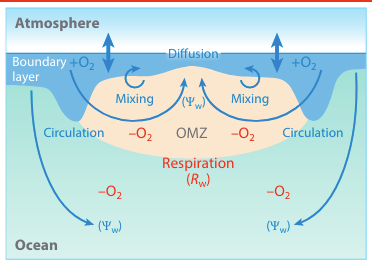
\includegraphics[width=0.48\textwidth]{Fig_OMZ}
		\caption[Oxygen circulation]{\footnotesize{Oxygen sources and sinks in the ocean, adapted from \autocite{Deutsch2024}. The Oxygen Minimum Zone (OMZ) is relatively still, so circulation from surface waters does not bring it as much oxygen as the deep ocean. Photosynthesis and atmospheric diffusion increase the amount of oxygen in surface waters, and respiration decreases the amount of oxygen in the midwater and deep water.}}
		\label{OMZ}
		 %the special ToC caption is in square brackets. The \footnotesize makes the figure caption smaller
	\end{center}
\end{wrapfigure} 

As a result of ocean warming and deoxygenation, hypoxic events in which the oxygen concentration in water becomes low enough to harm or kill marine organisms are increasing in frequency, duration, and severity throughout the world's oceans. Because different species have different tolerances to hypoxia and different levels of mobility, not all species distributions will be affected in the same way by changing hypoxic conditions. This could have large effects on marine ecosystems through direct effects (e.g. mass die-offs of hypoxia sensitive species and hypoxia tolerant species becoming more prevalent) or indirect effects (e.g. offsets in predator and prey populations). Hypoxic conditions can force migrations between depths or geographic regions, which change the distribution of species \autocite{Deutsch2024, Pihl1991}. Thus, understanding the effects of this global decrease in ocean oxygen levels is crucial to predicting the overall effects of climate change on the oceans and to developing climate-aware management strategies for marine resources. 

\section{Study Location: OCNMS}

\subsection{Upwelling in OCNMS}

This study will focus on hypoxia in Olympic Coast National Marine Sanctuary (OCNMS), off the coast of Washington state, U.S.A.. The Olympic Coast is the California Current Eastern boundary current upwelling zone, meaning that when summer winds push the surface water offshore, nutrient-rich and oxygen-poor water flows upwards from the 150-200m deep waters of the Pacific Ocean towards the coast (see Figure \ref{Upwelling}), \autocite{OfficeofNationalMarineSanctuaries2022, Hickey2003}. After this oxygen-poor water is advected onto the shallower waters of the continental shelf, respiration of decaying organic matter further reduces the water's oxygen content, leading to hypoxia in the bottom of the water column \autocite{Pierce2012, Landry1989}. Another major cause of hypoxia worldwide is eutrophication, which occurs when nutrient runoff results in a sudden population boom in phytoplankton, which then die and decompose, leading to a rapid decrease in dissolved oxygen levels \autocite{Deutsch2024}. However, eutrophication is not a major driver of hypoxia in OCNMS \autocite{OfficeofNationalMarineSanctuaries2022}.

Nutrients from upwelling sustain a rich ecosystem with high primary productivity, but as oceans warm and the deep water gets progressively more hypoxic, the seasonal hypoxic events in OCNMS are increasing in their severity and duration, which will eventually harm organisms more than the nutrients help them. Additionally, as climate change warms the land and ocean at different rates, the summer winds that cause upwelling are getting stronger, resulting in upwelling events that push more deep water up towards the coast \autocite{Barth2024}. Eastern boundary current upwelling zones are being affected by climate change in a variety of complex ways, so studying the effects of extreme oceanographic conditions in an upwelling zone in detail will inform our future understanding of how these extremely productive ecosystems will respond to climate change \autocite{Bograd2023}.

\begin{figure}[!h]
	\begin{center}
		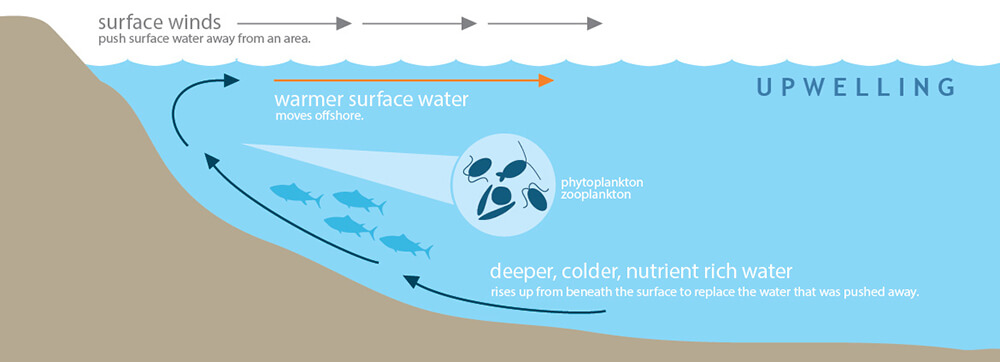
\includegraphics[scale=0.4]{Fig_NOAA_Upwelling}
		\caption[Upwelling]{\footnotesize{In the summer, winds move warmer surface water offshore, resulting in cold, nutrient-rich water flowing upwards into OCNMS. Image: NOAA, from \autocite{OceanographyOlympicCoast}.}} %the special ToC caption is in square brackets. The \footnotesize makes the figure caption smaller
		\label{Upwelling}
	\end{center}
\end{figure} 

Hypoxic events have been observed annually in the US Pacific Northwest since 2002, and their increasing size and severity has been linked to climate change \autocite{Bograd2023, Parks2009}. These events have led to fish and crabs dying in large numbers, as well as moving to shallower waters temporarily \autocite{Grantham2004}. According to Barth et al. 2024, the hypoxic fraction of near-bottom water inshore of the 200-m isobath increased from 2\% to 24\% between their two comparison periods, 1950-1980 and 2009-2018. During the first year of this study, 2021, this hypoxic fraction increased to 56\% due to extreme upwelling conditions \autocite{Barth2024}. 

\subsection{OCNMS Ecosystems and Policies}

\begin{wrapfigure}{r}{0.5\textwidth}
	\begin{center}
		\includegraphics[width=0.48\textwidth]{Fig_OCNMS_Map}
		\caption[Map of OCNMS]{\footnotesize{The coast of Washington State with the border of Olympic National Marine Sanctuary (OCNMS) in red. Image from \fullcite{OlympicCoastNationalb}.}} %the special ToC caption is in square brackets. The \footnotesize makes the figure caption smaller
		\label{OCNMSMap}
	\end{center}
\end{wrapfigure} 

OCNMS is located off the Olympic Peninsula of Washington state, and extends 25 to 45 miles into the ocean. It regularly experiences rough seas, wave heights up to 49 feet, and intense winter storms. The sanctuary contains a wide variety of habitats, including rocky shores, kelp forests, sandy seafloor, and deep ocean canyons. The sanctuary is home to many marine mammals, fish, invertebrates, and seaweeds, and is a major feeding area for migrating seabirds. The sanctuary protects habitat for rockfish, salmon, halibut, Dungeness crab and other ecologically, commercially, and culturally important species of the Olympic Coast \autocite{OfficeofNationalMarineSanctuaries2022}.  Within the sanctuary, many activities that could damage the ocean environment are prohibited, such as moving or injuring historical resources, certain waste discharge from boats, military bombing activities, seabed drilling, and oil, gas, and mineral development. Activities that could harm wildlife, such as taking or disturbing marine mammals and birds, are also prohibited \autocite{15CFRPart1995}. The Olympic Coast National Marine Sanctuary Advisory Council provides advice on the sanctuary's management. The council is comprised of tribal, federal, state, and local government representatives, as well as local industries and interests including maritime industry, fishing, education, tourism, and conservation. The sanctuary lies within the Usual and Accustomed treaty fishing, hunting, and gathering areas of the Hoh Tribe, Makah Tribe, Quileute Tribe, and the Quinault Indian Nation, known collectively as the Coastal Treaty Tribes. Fisheries and other marine resources off the Olympic Coast are co-managed by the state of Washington, the United States (specifically the National Oceanographic and Atmospheric Administration's Office of National Marine Sanctuaries), and the Coastal Treaty Tribes, who formed the Olympic Coast Intergovernmental Policy Council (IPC) in 2007 to provide a forum for resource managers \autocite{IntergovernmentalPolicyCouncil}.


\section{Copepods}

Copepods are crustacean zooplankton of the class Copepoda, formerly combined with the class Thecostraca under the class Hexanauplia \autocite{Oakley2013, Lozano-Fernandez2019}. Copepods are abundant in nearly every body of water on Earth, including oceans, freshwater, groundwater, and New York City's tap water \autocite{Vakati2023, Berger2004}. They are an important component of marine and freshwater food chains, as they eat phytoplankton and are eaten by a wide variety of fish. This study will focus on free-living marine copepods found in OCNMS. In the northeast Pacific Ocean, copepods are important food sources for many pelagic fishes, including juvenile salmon \autocite{Brodeur1990}. Copepods are eaten by herring and juvenile salmon, especially chum and sockeye salmon, off the west coast of North America. \autocite{Brodeur1990, Friedenberg2012}. Because of their importance to the food chain, especially as prey for culturally and economically important fish such as salmon, it is important to understand how copepod populations are affected by hypoxic events, and how they might be affected by worsening hypoxia in the future as climate change intensifies. 

\subsection{Seasonal Classifications}

The copepod species most commonly found in OCNMS are classified as Northern (cold-water) and Southern (warm-water) based on their seasonal pattern of occurrence (See Table \ref{CopepodGroups}, \autocite{NOAAFisheries2024, Peterson2003, Peterson1977}). Northern copepods are more common in the summer, and southern copepods are more common in the winter \autocite{NOAAFisheries2024}.  In studies of the Oregon coast, which is part of the same California Current upwelling system as OCNMS, \textit{Pseudocalanus}, \textit{Acartia}, \textit{Oithona} and \textit{Calanus} were the dominant genera in the summer, while \textit{Paracalanus} and \textit{Ctenocalanus} dominated in the winter \autocite{Peterson1977, Peterson2003}. Northern copepods, especially Calanus marshalls and Pseudocalanus mimus, are known to be more lipid-rich. These fattier copepods serve as important food sources for salmon populations \autocite{NOAAFisheries2024}. Copepod species richness in the coastal Northeast Pacific Ocean is generally lower in the summer, and copepod biomass off the Oregon coast is highest in the summer \autocite{Peterson2003}. 

\begin{table}	
	\begin{center} 
		\begin{tabular}{l l}  
			\toprule
			Species &  Group \\ 
			\midrule 
			\textcolor{RoyalBlue}{\textit{Acartia clausii}} & 	\textcolor{RoyalBlue}{Cold-water} 	 \\ 
			\textcolor{RoyalBlue}{\textit{Acartia longiremis}}	& \textcolor{RoyalBlue}{Cold-water}  \\
			\textcolor{RoyalBlue}{\textit{Calanus marshallae}}	& \textcolor{RoyalBlue}{Cold-water}  \\
			\textcolor{RoyalBlue}{\textit{Centropages abdominales}}	& \textcolor{RoyalBlue}{Cold-water}  \\
			\textcolor{RoyalBlue}{\textit{Microcalanus pusillus}}	& \textcolor{RoyalBlue}{Cold-water}  \\
			\textcolor{RoyalBlue}{\textit{Pseudocalanus mimus}} & \textcolor{RoyalBlue}{Cold-water}  \\
			\textcolor{RoyalBlue}{\textit{Pseudocalanus acuspes}} & \textcolor{RoyalBlue}{Cold-water}  \\
			\textcolor{RoyalBlue}{\textit{Pseudocalanus spp.}} & \textcolor{RoyalBlue}{Cold-water}  \\
			\textit{Oithona similis}	& Year-round  \\
			\textcolor{RedOrange}{\textit{Acartia tonsa}}	& \textcolor{RedOrange}{Warm-water}  \\
			\textcolor{RedOrange}{\textit{Calanus pacificus}}	& \textcolor{RedOrange}{Warm-water}  \\
			\textcolor{RedOrange}{\textit{Calocalanus spp.}}	& \textcolor{RedOrange}{Warm-water}  \\
			\textcolor{RedOrange}{\textit{Clausocalanus spp.}} & \textcolor{RedOrange}{Warm-water}  \\
			\textcolor{RedOrange}{\textit{Clausocalanus parapergens}} & \textcolor{RedOrange}{Warm-water}  \\
			\textcolor{RedOrange}{\textit{Ctenocalanus vanus}}  & \textcolor{RedOrange}{Warm-water}  \\
			\textcolor{RedOrange}{\textit{Metridia pacifica}}	& \textcolor{RedOrange}{Warm-water}  \\
			\textcolor{RedOrange}{\textit{Paracalanus spp.}}	& \textcolor{RedOrange}{Warm-water}  \\
			\textcolor{RedOrange}{\textit{Paracalanus parvus}} & \textcolor{RedOrange}{Warm-water}  \\
			\bottomrule 
		\end{tabular}
		% square brackets --> Table of Tables. curly braces --> caption over the table.
		 % to reference this table, write \ref{CopepodGroups}
		\caption[Seasonal classification of copepods]{Classification of copepods as cold-water (``Northern," primarily occurring in the summer upwelling season) and warm-water (``Southern," primarily occurring in the winter) \autocite{NOAAFisheries2024, Peterson2003, Peterson1977}}\label{CopepodGroups}  % need to add in proper citations
	\end{center}
\end{table}

\subsection{Effects of Hypoxia on Copepods}

Previous lab work on copepod hypoxia tolerance has found that dissolved oxygen levels below 0.9-1.5 mg/L can kill many copepods within days, and levels below 0.66-0.9 mg/L kill nearly all copepods \autocite{He2021, Marcus2004, Stalder1997, Grodzins2016}. However, hypoxia exposure was not found to impact the common model species \textit{Acartia tonsa}'s eggs \autocite{Invidia2004}. Oxygen levels above 1.7 mg/L are generally safe for copepods \autocite{Grodzins2016}. In lab experiments by He et al., copepods have been observed to behaviorally avoid dissolved oxygen levels between 1.0 and 2.0 mg/L, although other experiments by Marcus \& Stalder did not find this pattern \autocite{He2021, Stalder1997}. In Puget Sound, an estuary very close to OCNMS, lower \textit{in situ} copepod abundance was observed at sites with dissolved oxygen concentrations of 2 mg/L or lower, and copepods were observed to behaviorally avoid dissolved oxygen levels below 2 mg/L by migrating vertically \autocite{Keister2020, Keister2013}. 

\begin{wrapfigure}{r}{0.6\textwidth}
	\begin{center}
		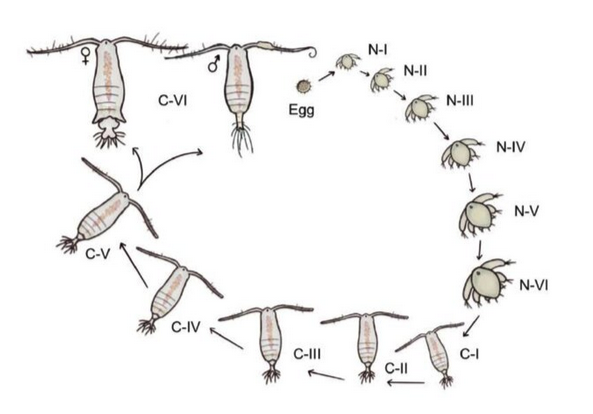
\includegraphics[width=0.58\textwidth]{Fig_Life_cycle}
		\caption[Life cycle of copepods]{\footnotesize{Simplified \textit{Paracartia grani} life cycle, not to scale. N: nauplius, C: copepodite. Copyright C. Traboni. \fullcite{Traboni2022}}} %the special ToC caption is in square brackets. The \footnotesize makes the figure caption smaller
		\label{LifeCycle}
	\end{center}
\end{wrapfigure} 

Even at nonlethal levels from 2.0-3.0 mg/L of dissolved oxygen, moderate hypoxia lowers copepod egg production, egg survival, and prey consumption. Egg production was delayed and reduced in lab studies that exposed copepods to 2.0 mg/L, 1.0 mg/L and 0.7 mL/L \autocite{Marcus2004, Richmond2006, Roman1993}. This may be because energy reserves must be spent coping with the physiological effects of low oxygen instead of on egg production or digestion, and egg production is very energy-intensive \autocite{Marcus2004, Elliott2013, Lutz1992, Stalder1997, Roff1992}. At lower dissolved oxygen levels, studies have found that the copepods \textit{A. tonsa} and \textit{Temora turbinata} decrease their rate of feeding \autocite{He2021, Elliott2013}. 

Higher temperatures are also a source of stress for copepods, although copepod thermal tolerances are understudied \autocite{Sasaki2021}. Copepods are capable of rapid thermal acclimation, but they can still be harmed or killed by high enough temperatures, and copepods acclimated to lower temperatures have lower thermal tolerances \autocite{Sasaki2021, Hahn2024}.  Additionally, copepod body size decreases with increasing temperature \autocite{Hahn2024}.  In many copepod species acclimated to 15-20 ºC, about 50\% of the population will die at 25 ºC, but the present study is at a site where water temperatures typically range from 8-12 ºC \autocite{Sasaki2019, Sunar2021, Jiang2009}. One study on Baltic Sea \textit{Acartia hudsonica} copepods found that copepods collected in the winter from ~7 ºC water had a critical thermal maximum of 25-27 ºC, and the same copepods acclimated to 11 ºC had a critical thermal maximum around 28 ºC, so it is \autocite{Hahn2024}. The critical thermal maximum is defined at the temperature at which an individual is no longer capable of moving away from harmful conditions, eventually resulting in death. Therefore, it is likely that these copepods experience sublethal impacts at temperatures lower than 25 ºC, and that temperatures above that threshold are harmful to them. 

The physiological problems that copepods face in hypoxic conditions are exacerbated by warmer temperatures, as crustaceans in general consume oxygen more rapidly at higher temperatures \autocite{Vaquer-Sunyer2011}. A combination of heat and hypoxia results in a lower hypoxia tolerance in most marine taxa, because organisms' metabolisms accelerate at higher temperatures, increasing their demand for oxygen \autocite{Deutsch2024}. Therefore, the combination of dissolved oxygen and temperature is a major limiting factor to the geographical range of many marine species \autocite{Deutsch2015, Deutsch2020}. As global oceans warm and lose oxygen, it is important to understand the interaction between these two environmental stressors on a variety of marine organisms in order to understand possible future changes to marine ecosystems.

\clearpage 

\section{Environmental DNA}\label{IntroeDNA}

% From Zack: 

% There are a bunch of different eDNA approaches that fall into 3 broad categories that are worth mentioning here 1) targeted assays (qPCR/dPCR/CRISPR/LAMP) that are species specific and measure absolute DNA concentrations, 2) biodiversity assays (metabarcoding) that target multiple species at once (what we did here), and 3) metagenomics which looks at functional genes present in the environment (most relevant to microbial/phytoplankton work since that's msot of the DNA you recover)

Environmental DNA (eDNA) is the genetic material present in the environment, including extracellular DNA, fragments of cells and tissues, and entire small organisms \autocite{Taberlet2018}. In marine environments, eDNA can be filtered out of the water and sequenced to detect many different species present at the place and time where the water sample was collected. eDNA is a powerful tool for detecting multiple species at once with relatively little sampling effort. Although eDNA is a sensitive tool, it is important to note it cannot detect demographic information such as size, sex, and age. The general process of eDNA sampling begins by physically filtering seawater, then extracting and amplifying the resulting DNA and chromosome fragments using polymerase chain reaction (PCR) \autocite{Power2023}. eDNA metabarcoding is conducted using a set of  primers designed to target a conserved region of DNA that flanks a hyper variable region of DNA across a broad set of species, thus enabling taxonomic classification of the resulting barcodes. The sequence fragments are compared to a reference database of genes sequenced from known species, allowing the species present in the water column at the time of sampling to be taxonomically identified \autocite{Miya2022}.

eDNA studies may take multiple approaches to sequencing, depending on their goals. Targeted assays are species-specific and measure absolute DNA concentrations, metabarcoding assays target multiple species, and metagemonics looks at functional genes present in the environment. The goal of this study was to understand the overall community composition, and so eDNA samples were processed using metabarcoding methods in order to detect a wide variety of species.

eDNA metabarcoding results provide read abundances, or numbers of DNA fragments, but these are affected by PCR replication efficiency, so they are difficult to compare between different species and methods \autocite{Miya2022}. While it is difficult to get quantitative results from eDNA, it is possible to calculate a metric of relative abundance within species that accounts for the effects of amplification bias across taxa, known as eDNA index. Kelly et al. 2019 found that this index accurately captures trends in the biomass of detected organisms using simulations. eDNA index is calculated in two steps. First, the read counts of each species within a sample are used to calculate the proportional relative abundance of that species within the sample. Then, within each species, those relative abundances are all divided by the highest relative abundance for the species, so that the resulting eDNA index ranges from 0 to 1. After this, each species has one sample where it has an eDNA index of one, and that is the sample where that species was most abundant. This method cannot be used to compare different species, only to determine trends within each species \autocite{Kelly2019}.

% Here is how I wrote about this in a paper from a few years ago: We transformed the eDNA read counts into eDNA index scores according to Kelly et al. [65], which normalizes the read count per technical PCR replicate per species. This index was computed by first calculating the proportional relative abundance of each species in each technical PCR replicate. The relative abundance was then divided by the maximum relative abundance for a given species across all samples (e.g. highest observed abundance for Northern Anchovy is 15% of all total reads which serves as the denominator), yielding the eDNA index score, which ranges from 0 to 1 and allows for comparisons of relative abundance for specific taxa across samples. The goal of applying this transformation is to account for the effects of amplification bias across taxa [86–88].

%We acknowledge that such an approach loses information about relative abundance between taxa in a sample. In particular, this approach likely over-inflates the abundance of rare taxa [88]. However, recent metabarcoding frameworks have highlighted that the compositional nature of metabarcoding [89] alongside species-specific amplification biases [87, 90], impair our ability to make adequate inferences from raw sequence counts or proportions between taxa without ancillary information on either the underlying target taxa abundances or amplification efficiencies [87, 90–93]. Thus, in the absence of such information, we follow the conservative methods advised by Kelly, Shelton, and Gallego [88] and employ the eDNA index, erring on the side of amplification efficiency bias being the largest contributor to observed differences in read counts across fish species from eDNA samples [72, 87, 94].

Since 2021, the National Oceanic and Atmospheric Administration's Pacific Marine Environmental Laboratory (NOAA PMEL) Ocean Molecular Ecology (OME) lab has been collecting eDNA samples in OCNMS using a modified McLane phytoplankton and particulate sampler (PPS, see Figure \ref{PPS}).  The PPS was deployed for four, month-long intervals between May 2021 and August 2023, at the Teawhit Head 42 meter depth mooring (see Figure \ref{OCNMSbuoys}). This sampler collected, filtered, and preserved 1 L water samples every 36 hours using 0.4 micron filters. Filters were then taken off the sampler, preserved in 95\% ethanol, frozen, and taken to the lab. Additionally, some samples were taken using Niskin bottles during PPS deployment and recovery. These samples were filtered using Sterivex filters and a peristaltic pump. In total, 84 samples were collected in 2021, 122 in 2022, and 60 in 2023. 24 of these samples had three PCR technical replicates each, and replicates on the same date were combined for this study. eDNA was extracted from the samples according to the DNeasy Blood and Tissue Kit protocols with adaptations from Spens et al. 2017 \autocite{Spens2017}. The full protocol is available on the Ocean Molecular Ecology Zenodo \autocite{Weinrich2025}. This study focuses on copepods, and only uses data from the CO1 (mitochondrially encoded cytochrome c oxidase I, a common barcoding gene for studies on eukaryotes) primer. Amplified regions were sequenced using the  Leray F / mICOlinF forward primer and Folmer R / HCO2198 reverse primer, according to OME protocols \autocite{Gold2024, Spens2017}. The CO1 sequences were then matched to available reference genomes, resulting in species detection data that includes the number of reads (DNA strands) of each species detected.

\begin{figure}
	\centering
	\begin{minipage}{0.4\textwidth}
		\centering
		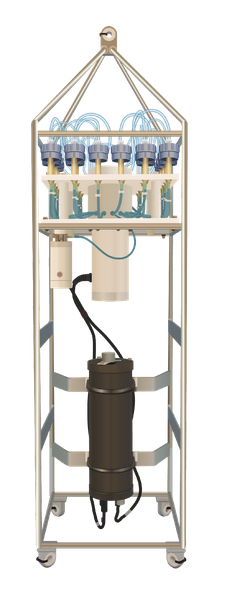
\includegraphics[width=0.7\linewidth]{Fig_PPS}
		\caption[Automated eDNA Sampler]{\footnotesize{Modified McLane phytoplankton and particulate sampler (PPS) used for automated eDNA sampling in OCNMS. This sampler was placed at TH042 (See Figure \ref{OCNMSbuoys}.)}}
		\label{PPS}
	\end{minipage}
	\hspace{1cm}
	\begin{minipage}{0.5\textwidth}
		\centering
		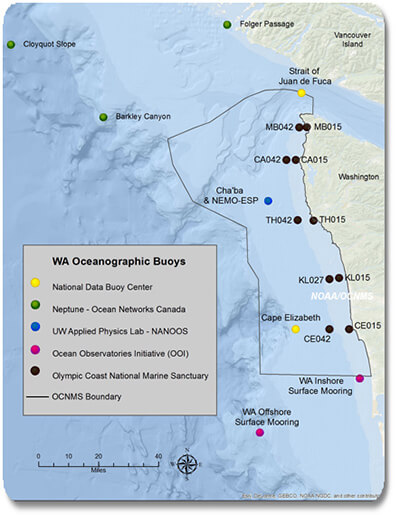
\includegraphics[width=1.0\linewidth]{Fig_OCNMS_buoy_map}
		\caption[Map of oceanographic moorings in OCNMS]{\footnotesize{Map of the Washington state coastline and Olympic Coast National Marine Sanctuary, featuring locations of Washington state oceanographic buoys. This study was conducted at the buoy labeled TH042 \fullcite{OceanographicMooringsOlympicb}}.}
		\label{OCNMSbuoys}
	\end{minipage}
\end{figure}

My summer 2024 research included combining the results of these eDNA detections with oceanographic measurements collected every ten minutes by the Teahwhit Head oceanographic mooring in 42 meter deep water (TH042), where the PPS sampler was deployed. I first matched the species detections to their associated metadata, including the sample date and time, using their unique sample IDs. I then matched each of those detections to the oceanographic mooring measurements that were closest to their sample date and time.  

\section{Study Plan}

Studies of the effects of hypoxia on marine organisms use a variety of lab and fieldwork methods. Laboratory experiments on hypoxia's effects typically involve subjecting organisms to different levels of dissolved oxygen over a certain period of time, then measuring factors such as survival, growth rate, metabolism, and reproductive rate in order to determine whether the hypoxia has a negative effect \autocite{Steckbauer2020}. Field studies typically entail measuring dissolved oxygen levels and organismal prevalence and abundance, using methods such as satellite tagging and trawl surveys that vary by scale and organism type (for example, \autocite{Keister2020}). Field experiments have more ecological relevance, but present difficulties in untangling the effects of other environmental factors \autocite{Borges2022, Boyd2018}. Therefore, linking experiments and field observations enables us to better demonstrate the connection between the lethal and sublethal effects of hypoxia shown in lab settings and real-world effects on organisms and changes in species distributions.

 Because copepods are so important to the OCNMS food web, further research into how these species respond to changes in dissolved oxygen and temperature is warranted \autocite{NOAAFisheries2024}. In this study, I will assess the effects of hypoxia on copepod abundance and community composition. I will compare copepod prevalence and eDNA index, a measure of relative abundance using eDNA detections, to dissolved oxygen data in order to assess whether hypoxia decreases copepod abundance in OCNMS. I will also generate preferred ranges of environmental conditions for each copepod species, and compare northern and southern copepod abundance across normoxic and hypoxic conditions. I predict that copepod abundance will decrease with hypoxia, and that the northern copepods will be detected in colder conditions than the southern copepods. Based on preliminary data analysis from the previous research, I expect southern copepods to persist at lower oxygen levels than northern copepods \autocite{Crotty2024}. Understanding these patterns will inform predictions of climate change effects on a foundational species of OCNMS food chains, which will inform predictions of the effects of climate change on entire OCNMS ecosystems.
	
    \chapter{Methods}
    
    % From Zack
    % And another: We then implemented a decontamination procedure to eliminate poorly sequenced samples and remove potential sources of contamination [44,52–54]. Importantly, we applied a site occupancy modeling framework to retain only ASVs that occurred in high prevalence across locations and stations. For these analyses, we removed all non-fish taxa from the resulting data. All remaining ASV’s had their read counts converted into the eDNA index [53]. The eDNA index transformation is conducted by first normalizing all reads for a particular sequence by the total number of reads in each sample, then scaling those proportions to the largest observed proportion for that sequence across all samples. This results in a sequence-specific (species-specific) scaling between 0 to 1, where 1 is the sample with the highest number of reads for a given species and 0 is the least.

	\section{eDNA Index Preparation}\label{MethodseDNA}
	Data analysis for this study was conducted using R version 4.3.0 ``Already Tomorrow." I downloaded eDNA sample data and environmental data from the TH042 mooring from previous OME research. Some \textit{P. mimus} samples were misidentified as \textit{P. acuspes}, so I re-identified the copepod sequence samples using NCBI BLAST and corrected the species identifications using those results. eDNA index was calculated in order to obtain a measure of the relative abundance of each species over time. Before calculating the eDNA index, I averaged the number of reads across technical replicates so that each observation represented one sampling date. Technical replicates included multiple samples taken at the same time, as well as multiple polymerase chain reaction (PCR) runs performed on the same sample. Additionally, each species has multiple characteristic variants of each gene that was used in the metabarcoding process, and each of those variants is called an ESV (Exact Sequence Variant). Because each individual observation in the data was one ESV, there were many observations of each species per sample. I combined these by adding up the total number of reads across all ESVs for each species in each sample. 
	
	\begin{figure}[!h]
		\begin{center}
			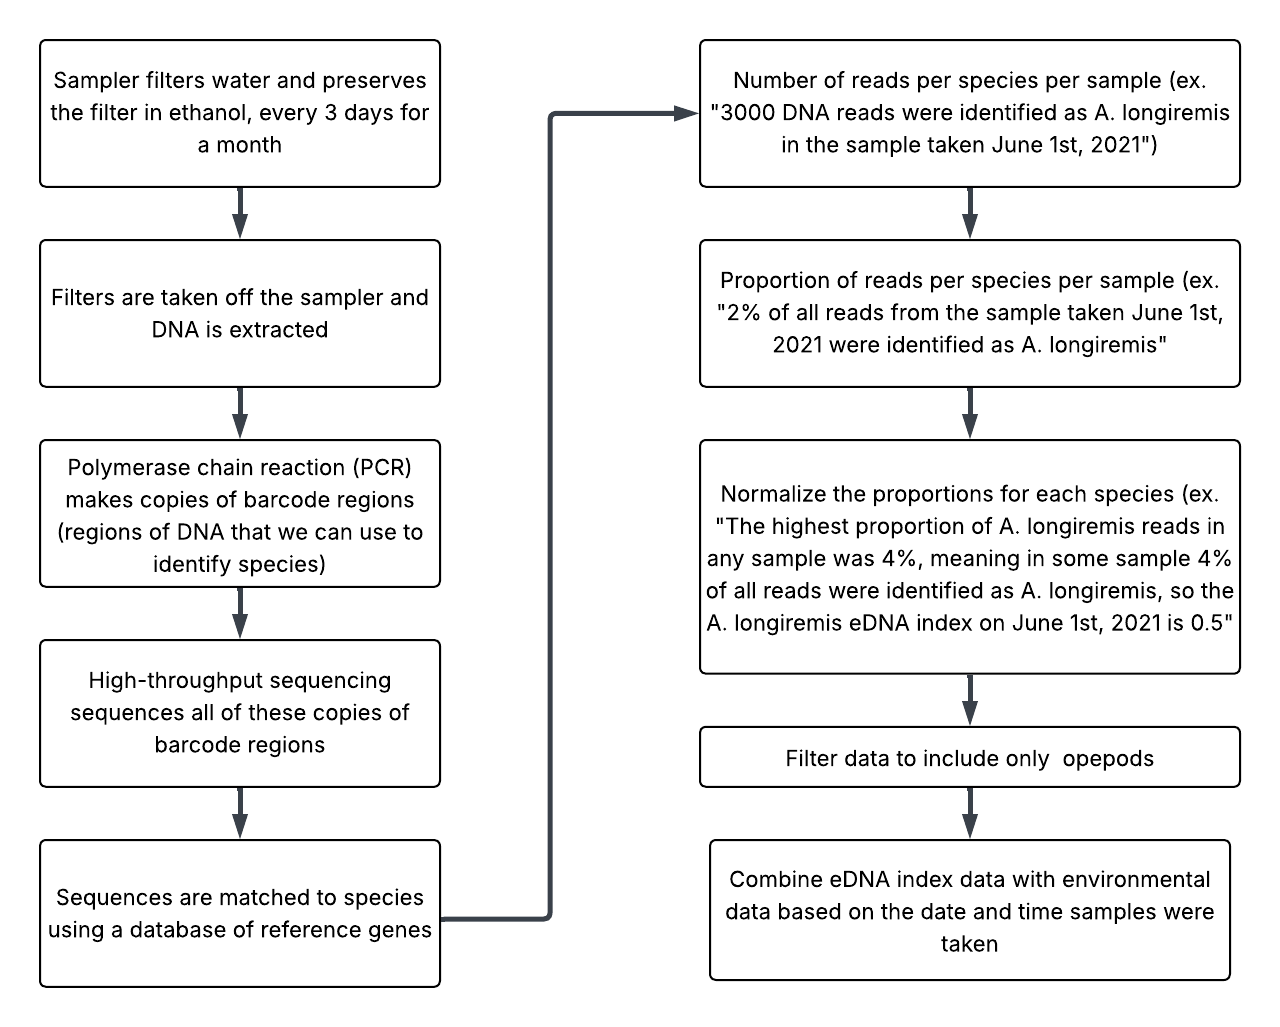
\includegraphics[scale=0.8]{Fig_MethodsFlowchart} \\
			\caption[Methods]{Flowchart detailing the steps to calculating eDNA index as laid out in sections \ref{IntroeDNA} and \ref{MethodseDNA}.} %the special ToC caption is in square brackets. The \footnotesize makes the figure caption smaller
			\label{Flowchart}
		\end{center}
	\end{figure} 
	
	I calculated eDNA index by grouping by sample, then calculating the proportion of reads of each species in each sample. I then normalized each species' proportions on a scale of 0 to 1, such that the sample with the most reads of that species had a value of 1, and any sample where that species was not detected had a value of 0. It is important to note that eDNA index cannot be used to make comparisons between species, but can be used to make comparisons between different time points in the same species. After calculating eDNA index, the data was filtered to only include copepods by selecting any observations in the genera \textit{Calocalanus}, \textit{Clausocalanus}, or \textit{Paracalanus}, as well as any observations in the class Hexanauplia, which contains Thecostraca and Copepoda (Oakley et al. 2013). While the class Hexanauplia is no longer recognized \autocite{WoRMSWorldRegister, Lozano-Fernandez2019}, and Thecostraca and Copepoda are now recognized as classes, it was used when the eDNA for this study was processed, so I used it for data processing as well. This study will not discuss species in Thecostraca.

	I combined the eDNA index data with its corresponding oceanographic data, using code from the previous study to attach each sample ID to its corresponding date and time, then joining it with the closest mooring observation. Additionally, I downloaded environmental data from the LiveOcean model at TH042 during the study period in order to fill in a data gap in 2023 during which the TH042 mooring was not functional, but the automated eDNA sampler was deployed \autocite{Siedlecki2015a, Fatland2016, LiveOceanHomepage}. I matched the LiveOcean model's hourly dissolved oxygen and temperature data to the eDNA sample data by date and time, and also compared the results of the LiveOcean model's 2021-22 data to the TH042 mooring's 2021-22 data. The model data matched the mooring data closely enough to be useable (See Figure \ref{ModelComparison}). When mooring and model data from the same hour was compared via linear model, the dissolved oxygen data had an R$^2$ value of 0.39 and a root mean square error (RMSE) of 0.98, and the temperature data had an R$^2$ of 0.82 and a RMSE of 0.41. The 2021-22 mooring-only data is still used for some of the statistical analyses in this thesis, as the mooring data captures short and extreme hypoxic events more accurately (See Figure \ref{ModelComparison}, orange spikes downwards are hypoxic events captured by the mooring but not the model). When modeling data is used in this thesis, it is used for all years 2021-23, in an effort to ensure that the different years are comprable and utilize all available eDNA sample dates. 
	
	\begin{wrapfigure}{r}{0.6\textwidth}
		\begin{center}
			a. 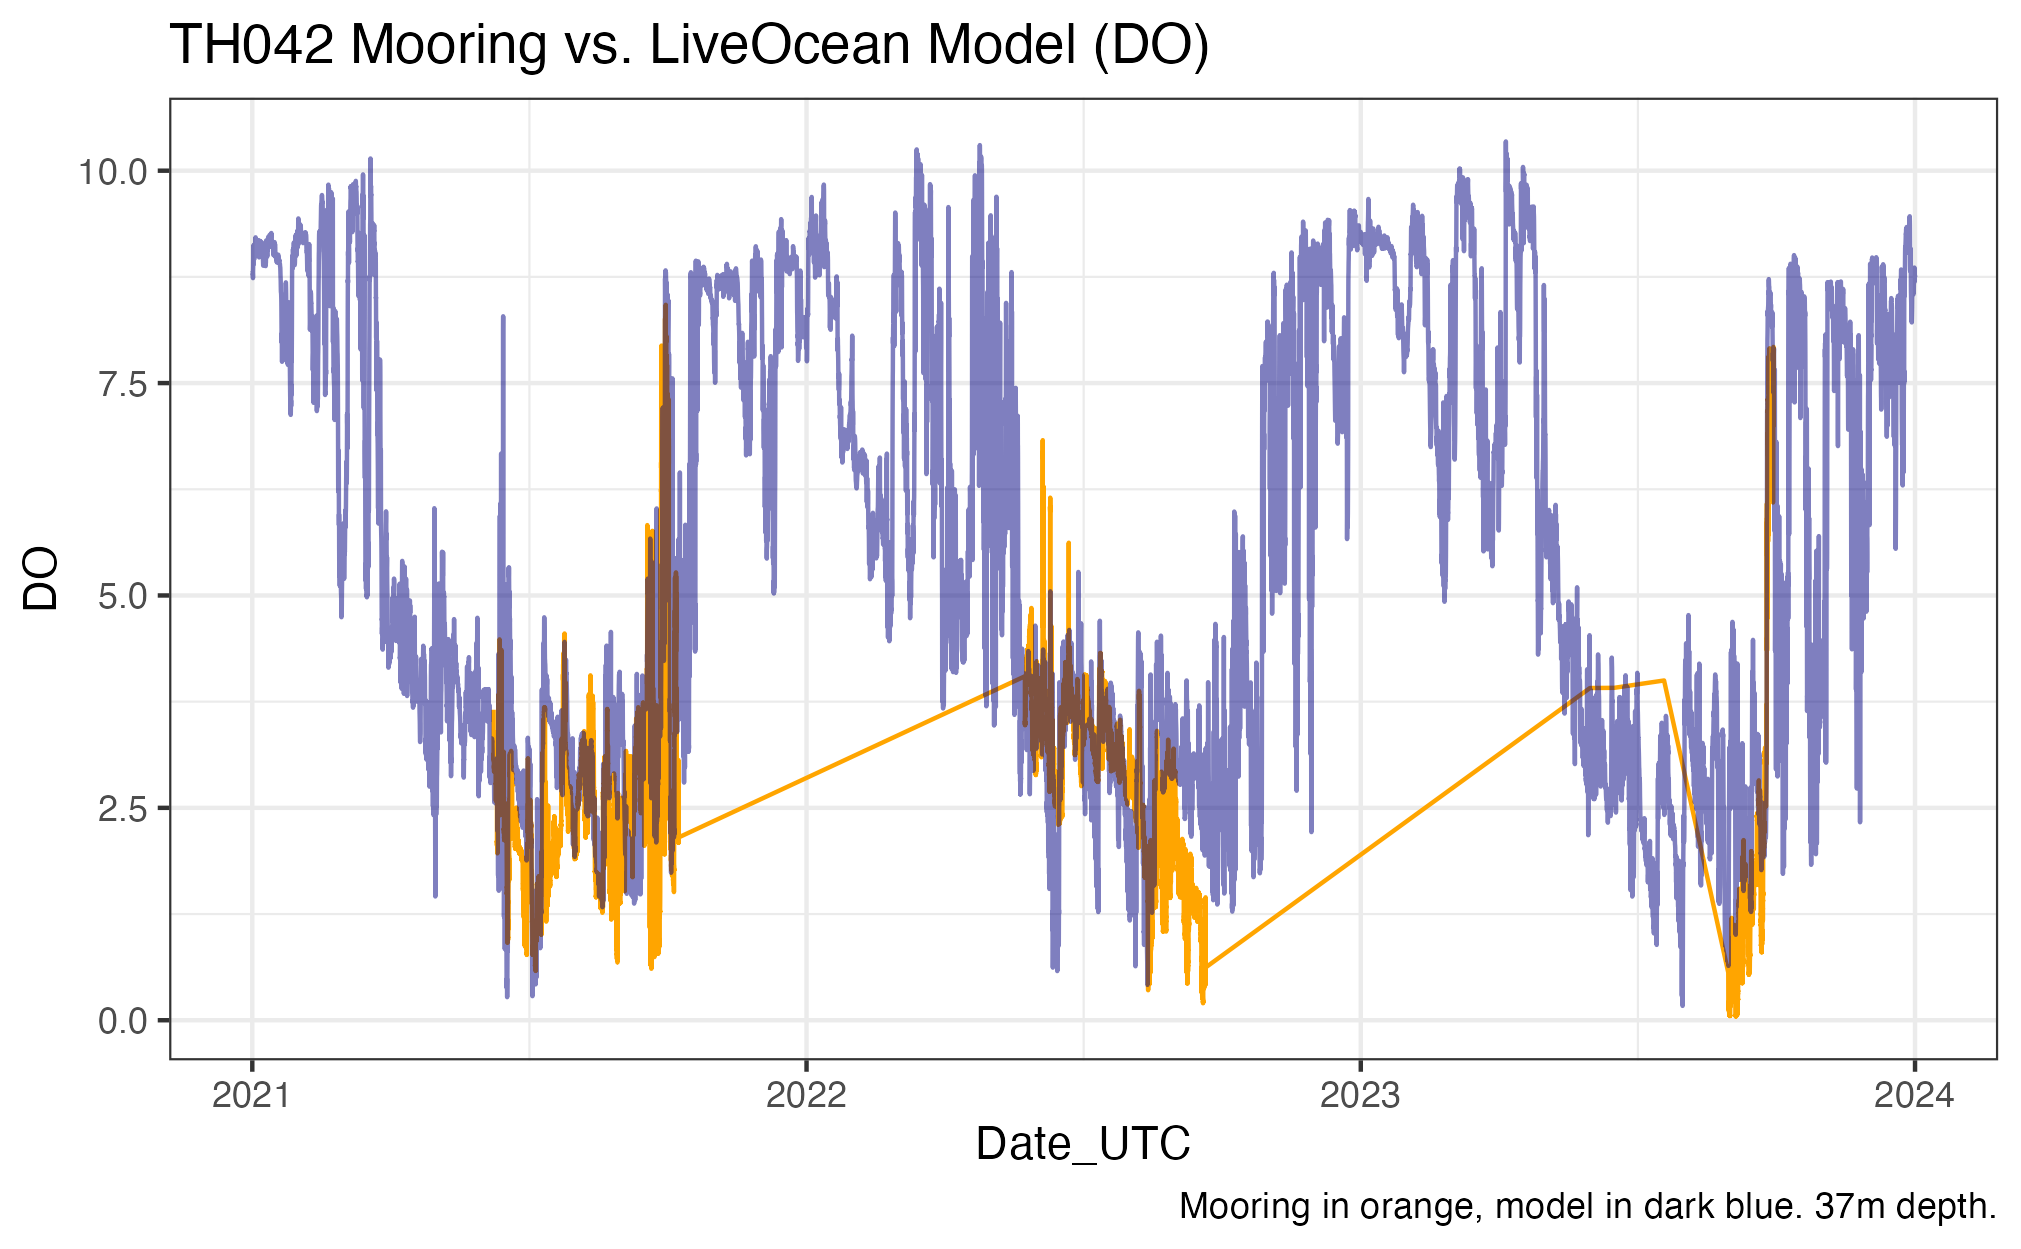
\includegraphics[width=0.58\textwidth]{Mooring_vs_Model_DO_37} \\
			b. 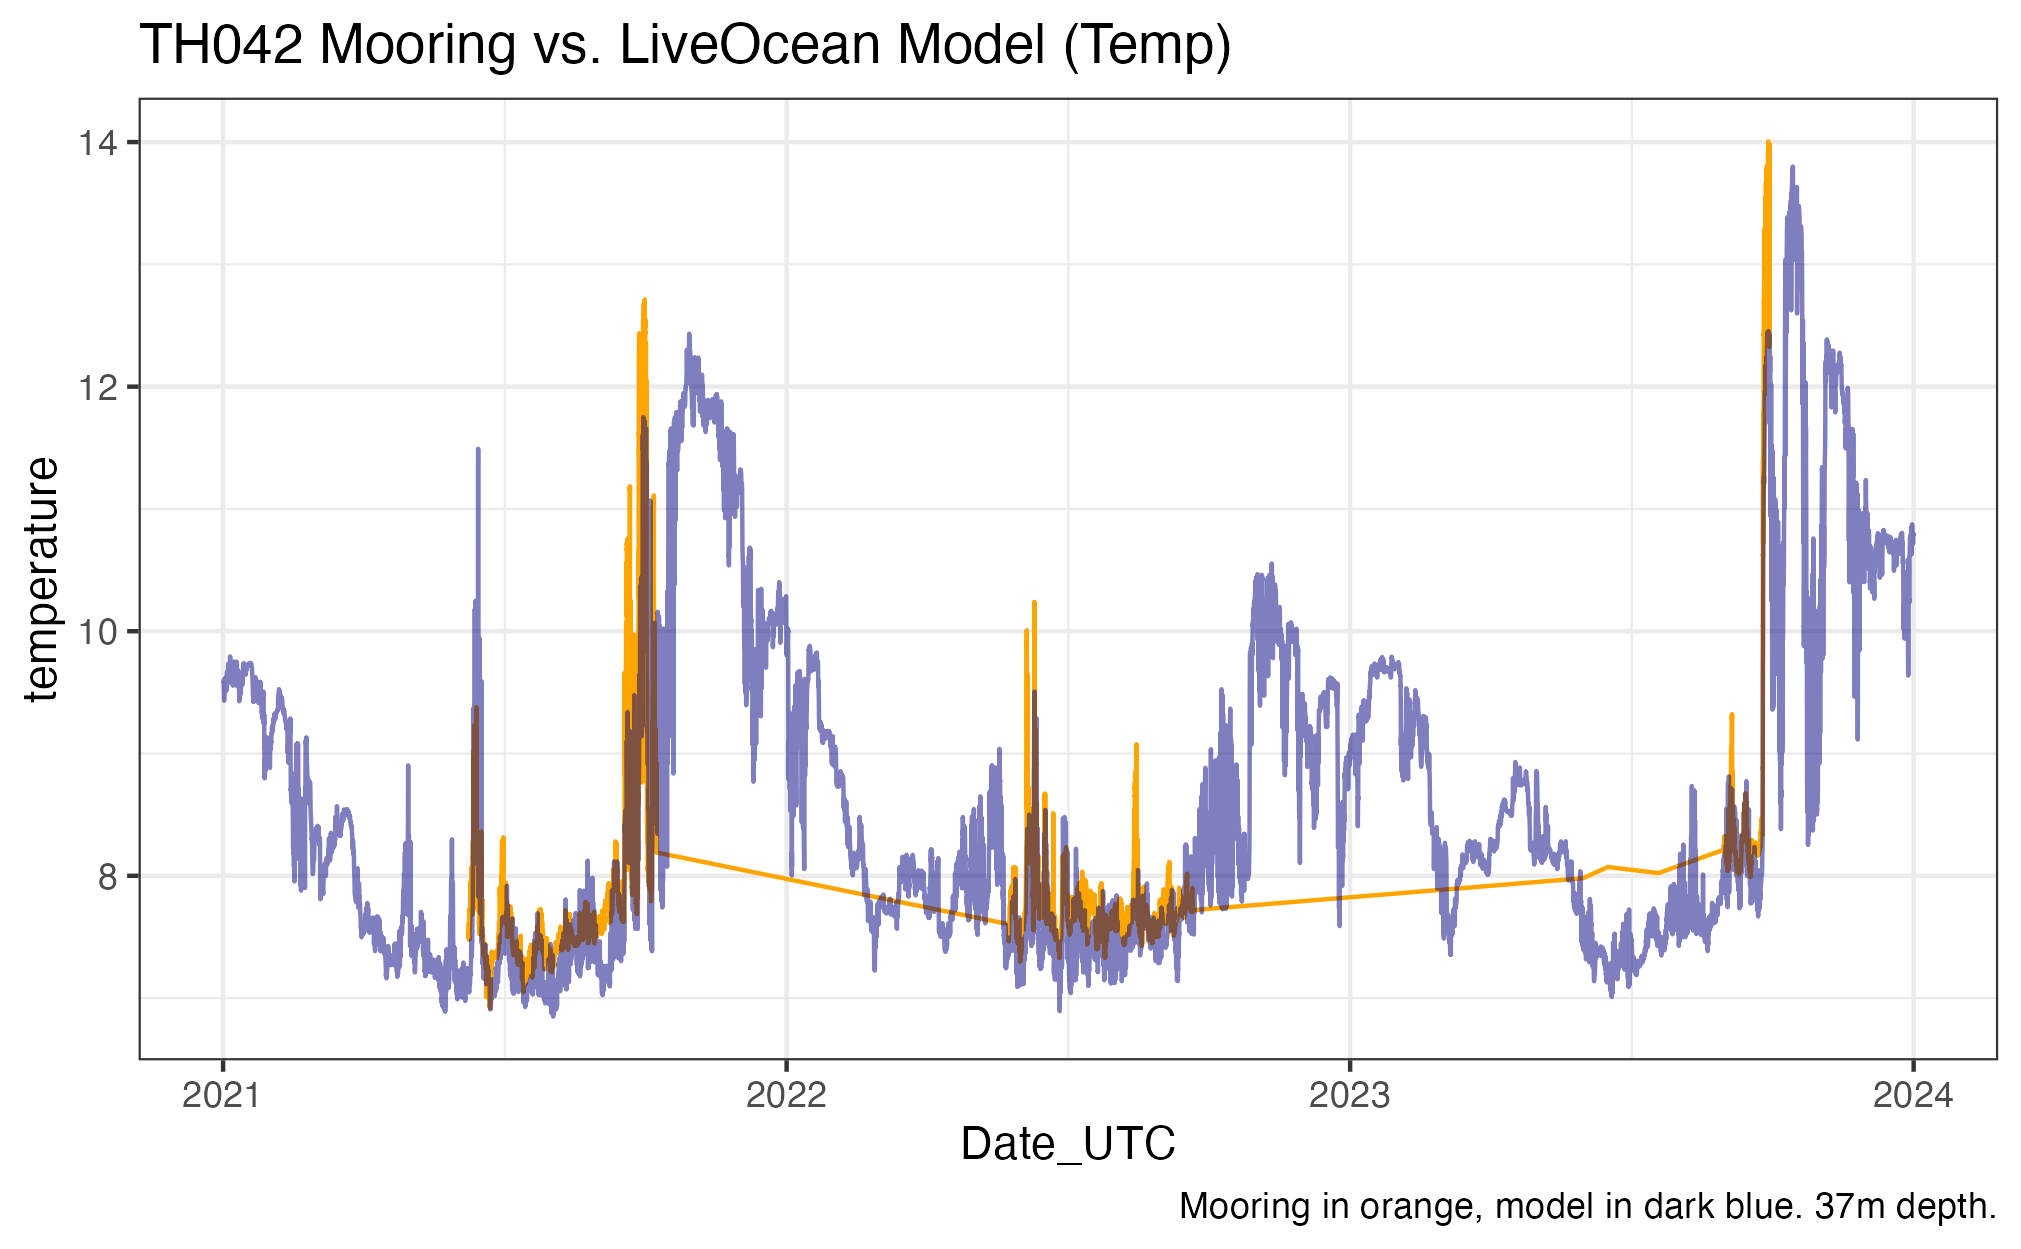
\includegraphics[width=0.58\textwidth]{Mooring_vs_Model_Temp_37}
			\caption[Mooring vs. Model Time Series]{Time series of (a) dissolved oxygen (mg/L) and (b) temperature (Celsius) over the study period. TH042 mooring data is displayed in orange, while LiveOcean model data is displayed in blue.} %the special ToC caption is in square brackets. The \footnotesize makes the figure caption smaller
			\label{ModelComparison}
		\end{center}
	\end{wrapfigure} 
	
	\begin{figure}[!h]
		\begin{center}
			a. 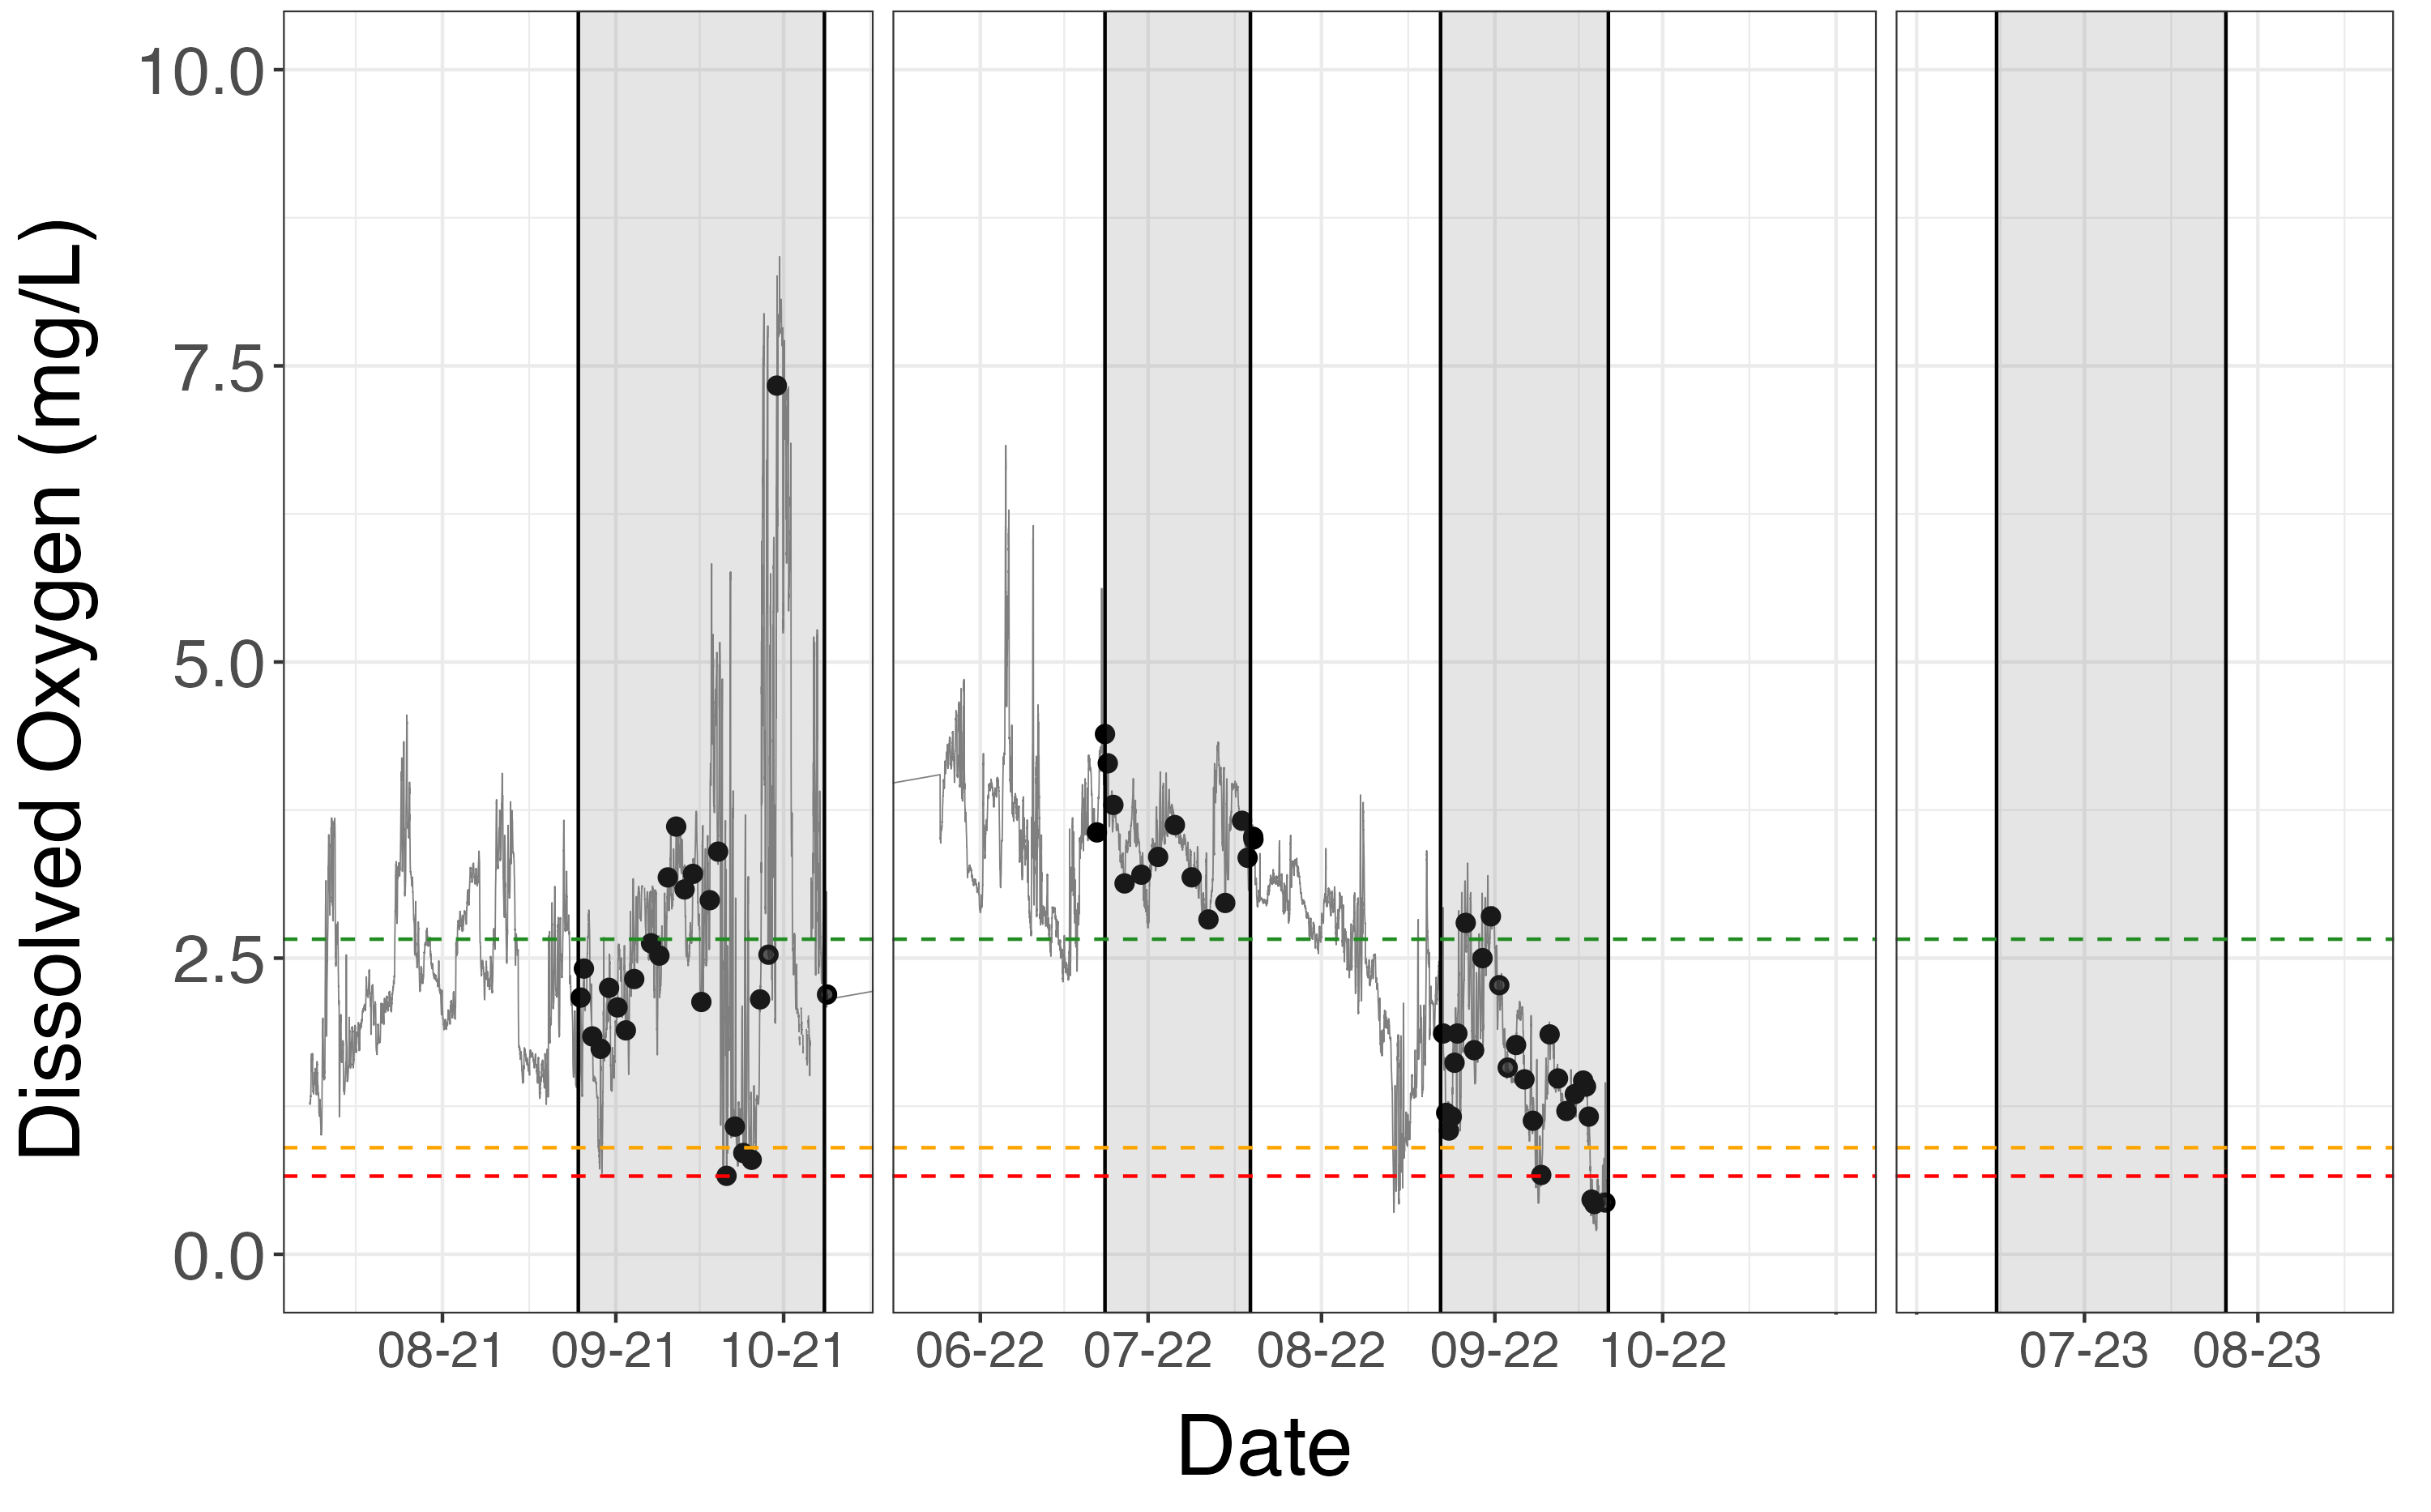
\includegraphics[scale=0.6]{Timeseries_example} \\
			b. 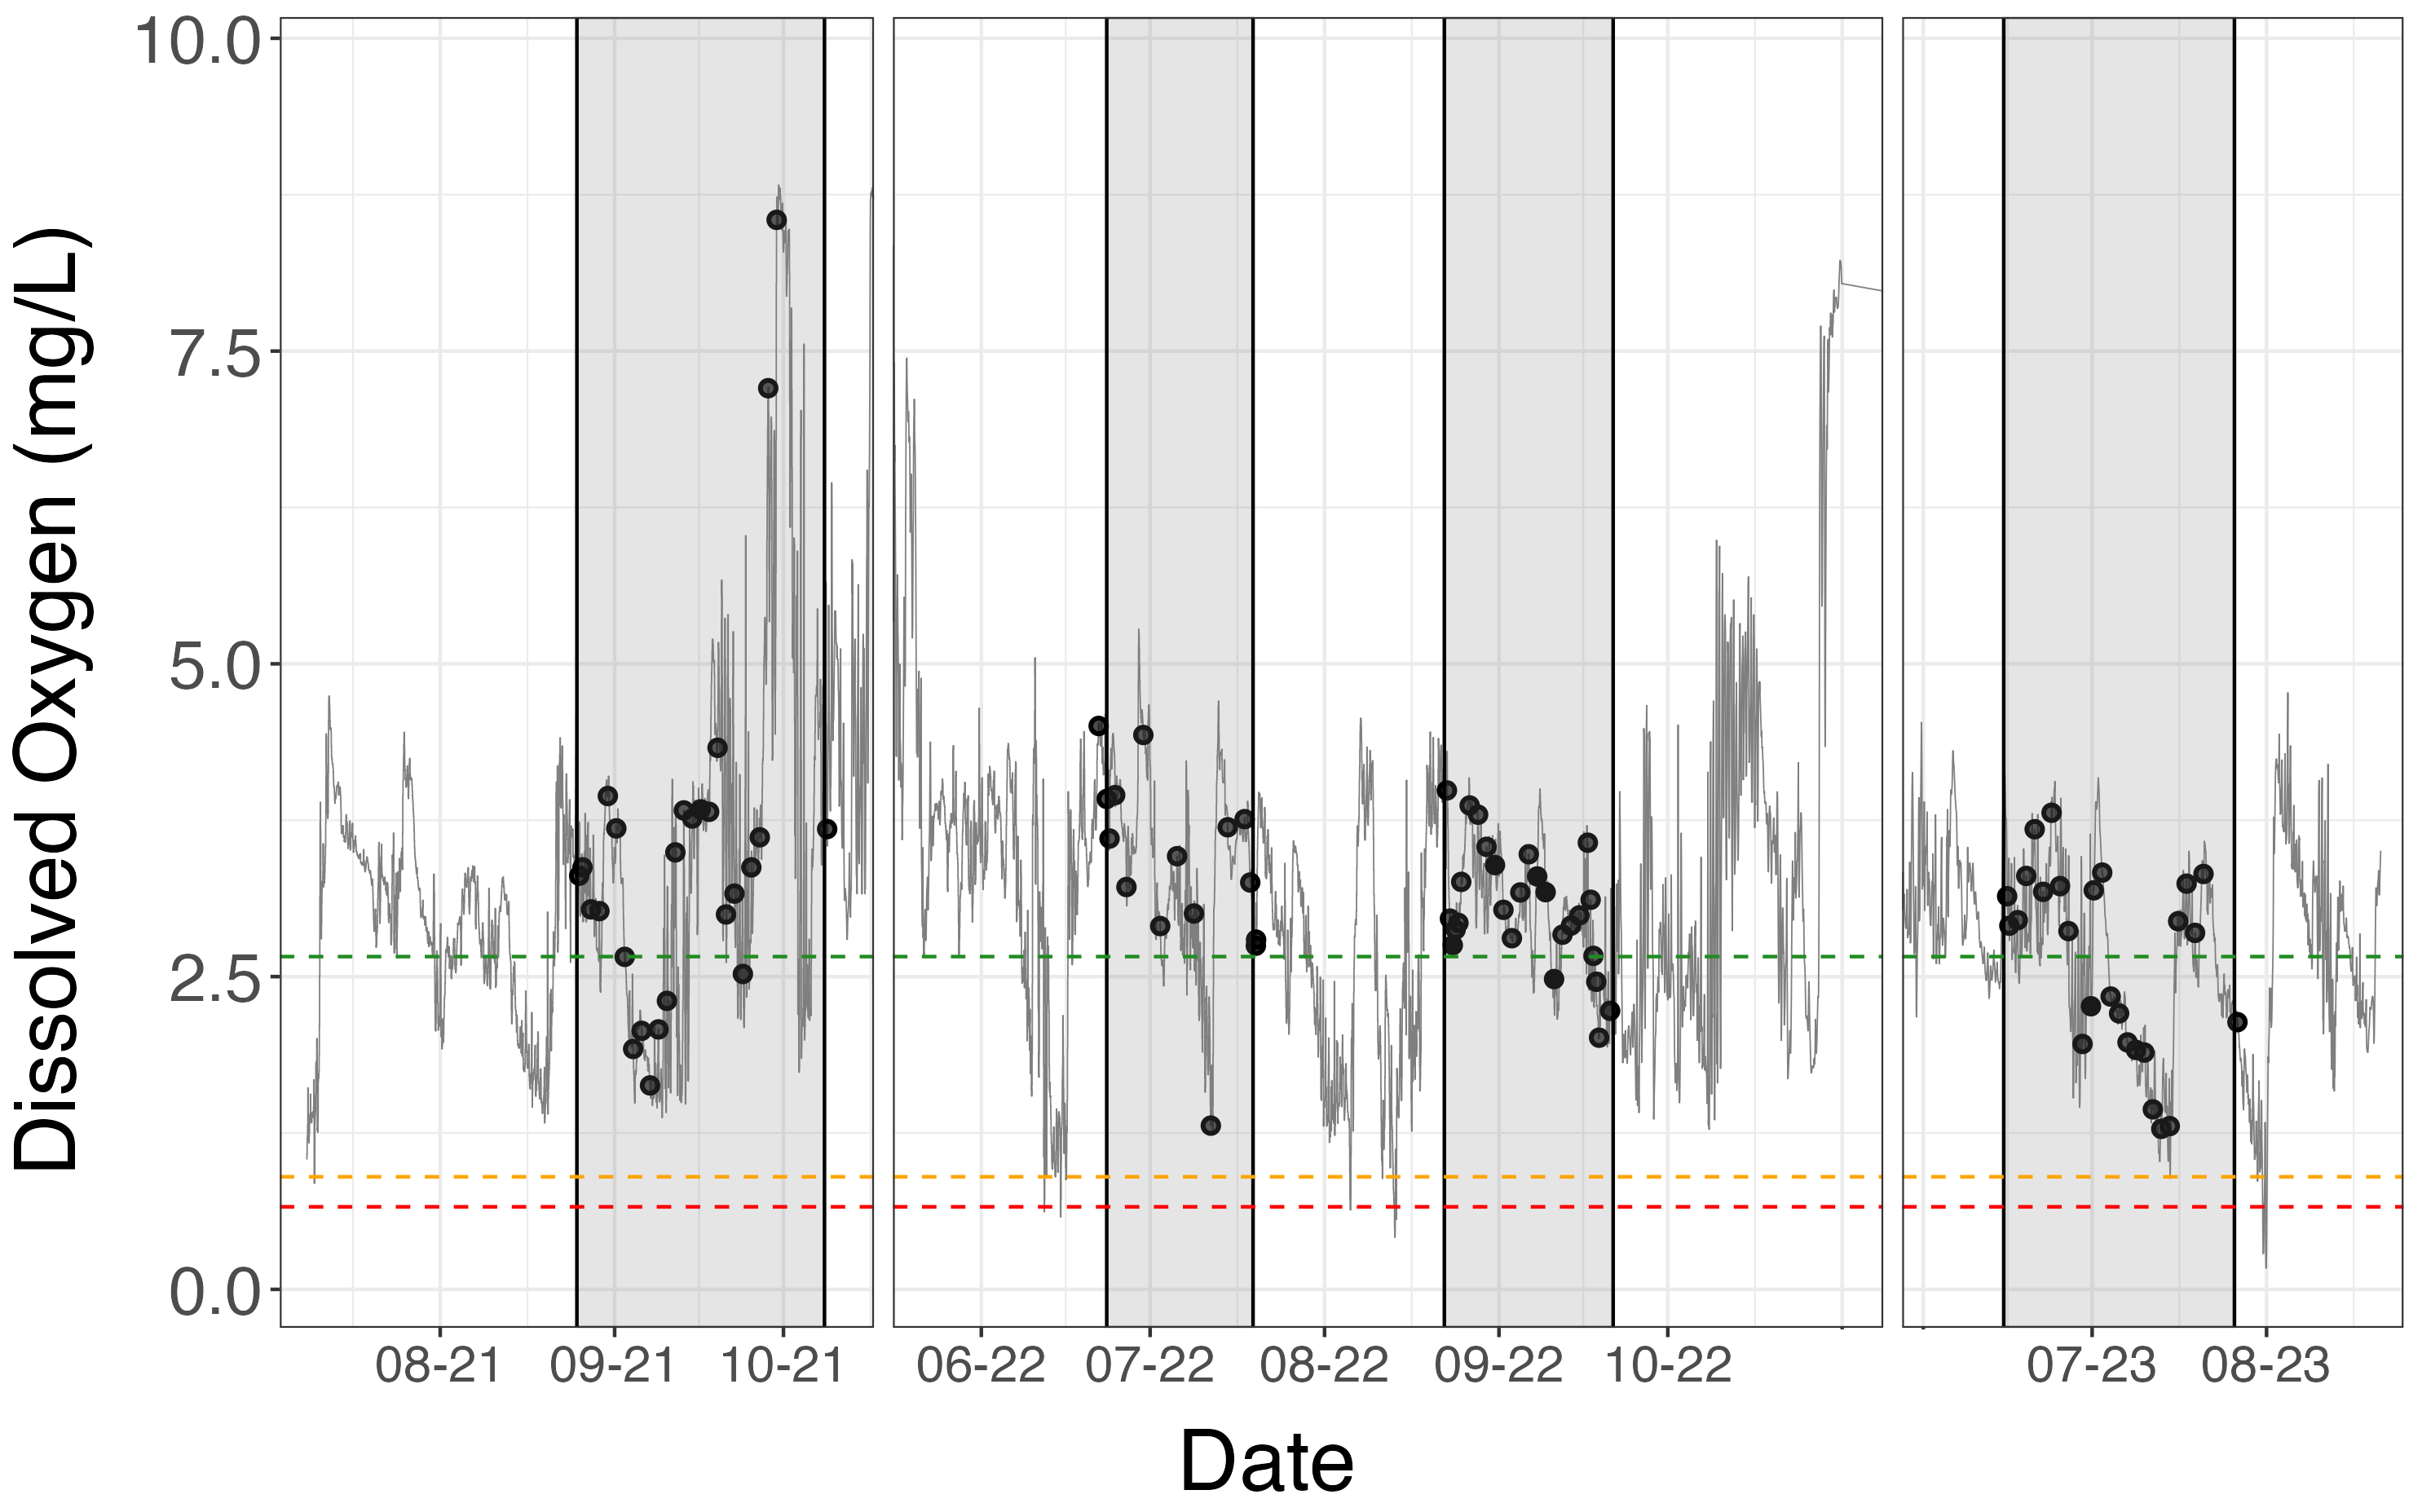
\includegraphics[scale=0.6]{Timeseries_example_Mod}
			\caption[Time series]{Time series of dissolved oxygen (mg/L) over the study period. Plot (a) displays TH042 mooring data, plot (b) displays LiveOcean model data. Black dots represent eDNA sampling dates. Gray boxes represent automated eDNA sampling periods. Red line represents 0.6 mg/L DO, a level known to kill most copepods in lab experiments, orange line represents 0.9 mg/L DO, a level known to kill approximately 50\% of copepods in lab experiments, and green line represents 2.66 mg/L DO, a level above which copepods have not shown negative effects in lab studies.} \label{Timeseries}%the special ToC caption is in square brackets. The \footnotesize makes the figure caption smaller
		\end{center}
		
	\end{figure} 
	
	\section{Data Visualization}
	In order to determine the relationships between copepod abundance and environmental factors, I compared eDNA index to temperature and dissolved oxygen. I conducted preliminary analysis using time series plots, where dissolved oxygen was plotted as a time series and each sample was plotted as a dot on top of the associated dissolved oxygen measurement (See Figure \ref{Timeseries}). This allowed for visual identification of hypoxic events in July 2021, October 2021, September 2022, and October 2023, as well as a heatwave in September 2021. Analysis of abundance relative to both dissolved oxygen and temperature was first conducted using scatterplots of dissolved oxygen and temperature at each sampling time, with color corresponding to eDNA index. To compensate for the different sampling frequencies in different environmental conditions, I then made density plots of the detection frequency within bins of environmental conditions, each spanning 0.5 mg/L of dissolved oxygen and 0.5 degrees Celsius. Each square of the plot represents a varying number of eDNA samples, and the darker squares have a higher proportion of species detections relative to non-detections. 
	
	In order to compare copepod hypoxia tolerances by size, I divided the species in the dataset into size bins based on the size ranges listed in the Marine Planktonic Copepods database \autocite{WoRMSWorldRegister}. Copepods with a minimum size smaller than 1.5 mm were classified as small, 1.5-2.5 mm copepods were classified as medium, 2.5-4 mm copepods were classified as large, and copepods exceeding 4 mm were classified as huge.
	
	\section{Statistical Analysis}
	I conducted statistical analyses of the relationship between species abundance and dissolved oxygen by using binomial regression models and zero-inflated beta regression models. I generated binomial regression models relating dissolved oxygen to species presence for each species of copepod in the dataset, excluding one data point that occurred during a short heatwave in September 2021. Because only one sample was taken during the heatwave and no other samples were from temperatures that high, it was difficult to draw conclusions about the effects of the heatwave on species presence, and the datapoint was excluded from the binomial regressions. Using the LiveOcean model data, two of the data points fell during the heatwave, because the model estimated that the heatwave started days earlier than the mooring indicated, and so those two sampling dates were excluded from statistical analyses. I then used the p-values for these binomial regressions to analyze individual species responses to hypoxia. 
	
	\begin{figure}[!h]
		\begin{center}
			a. 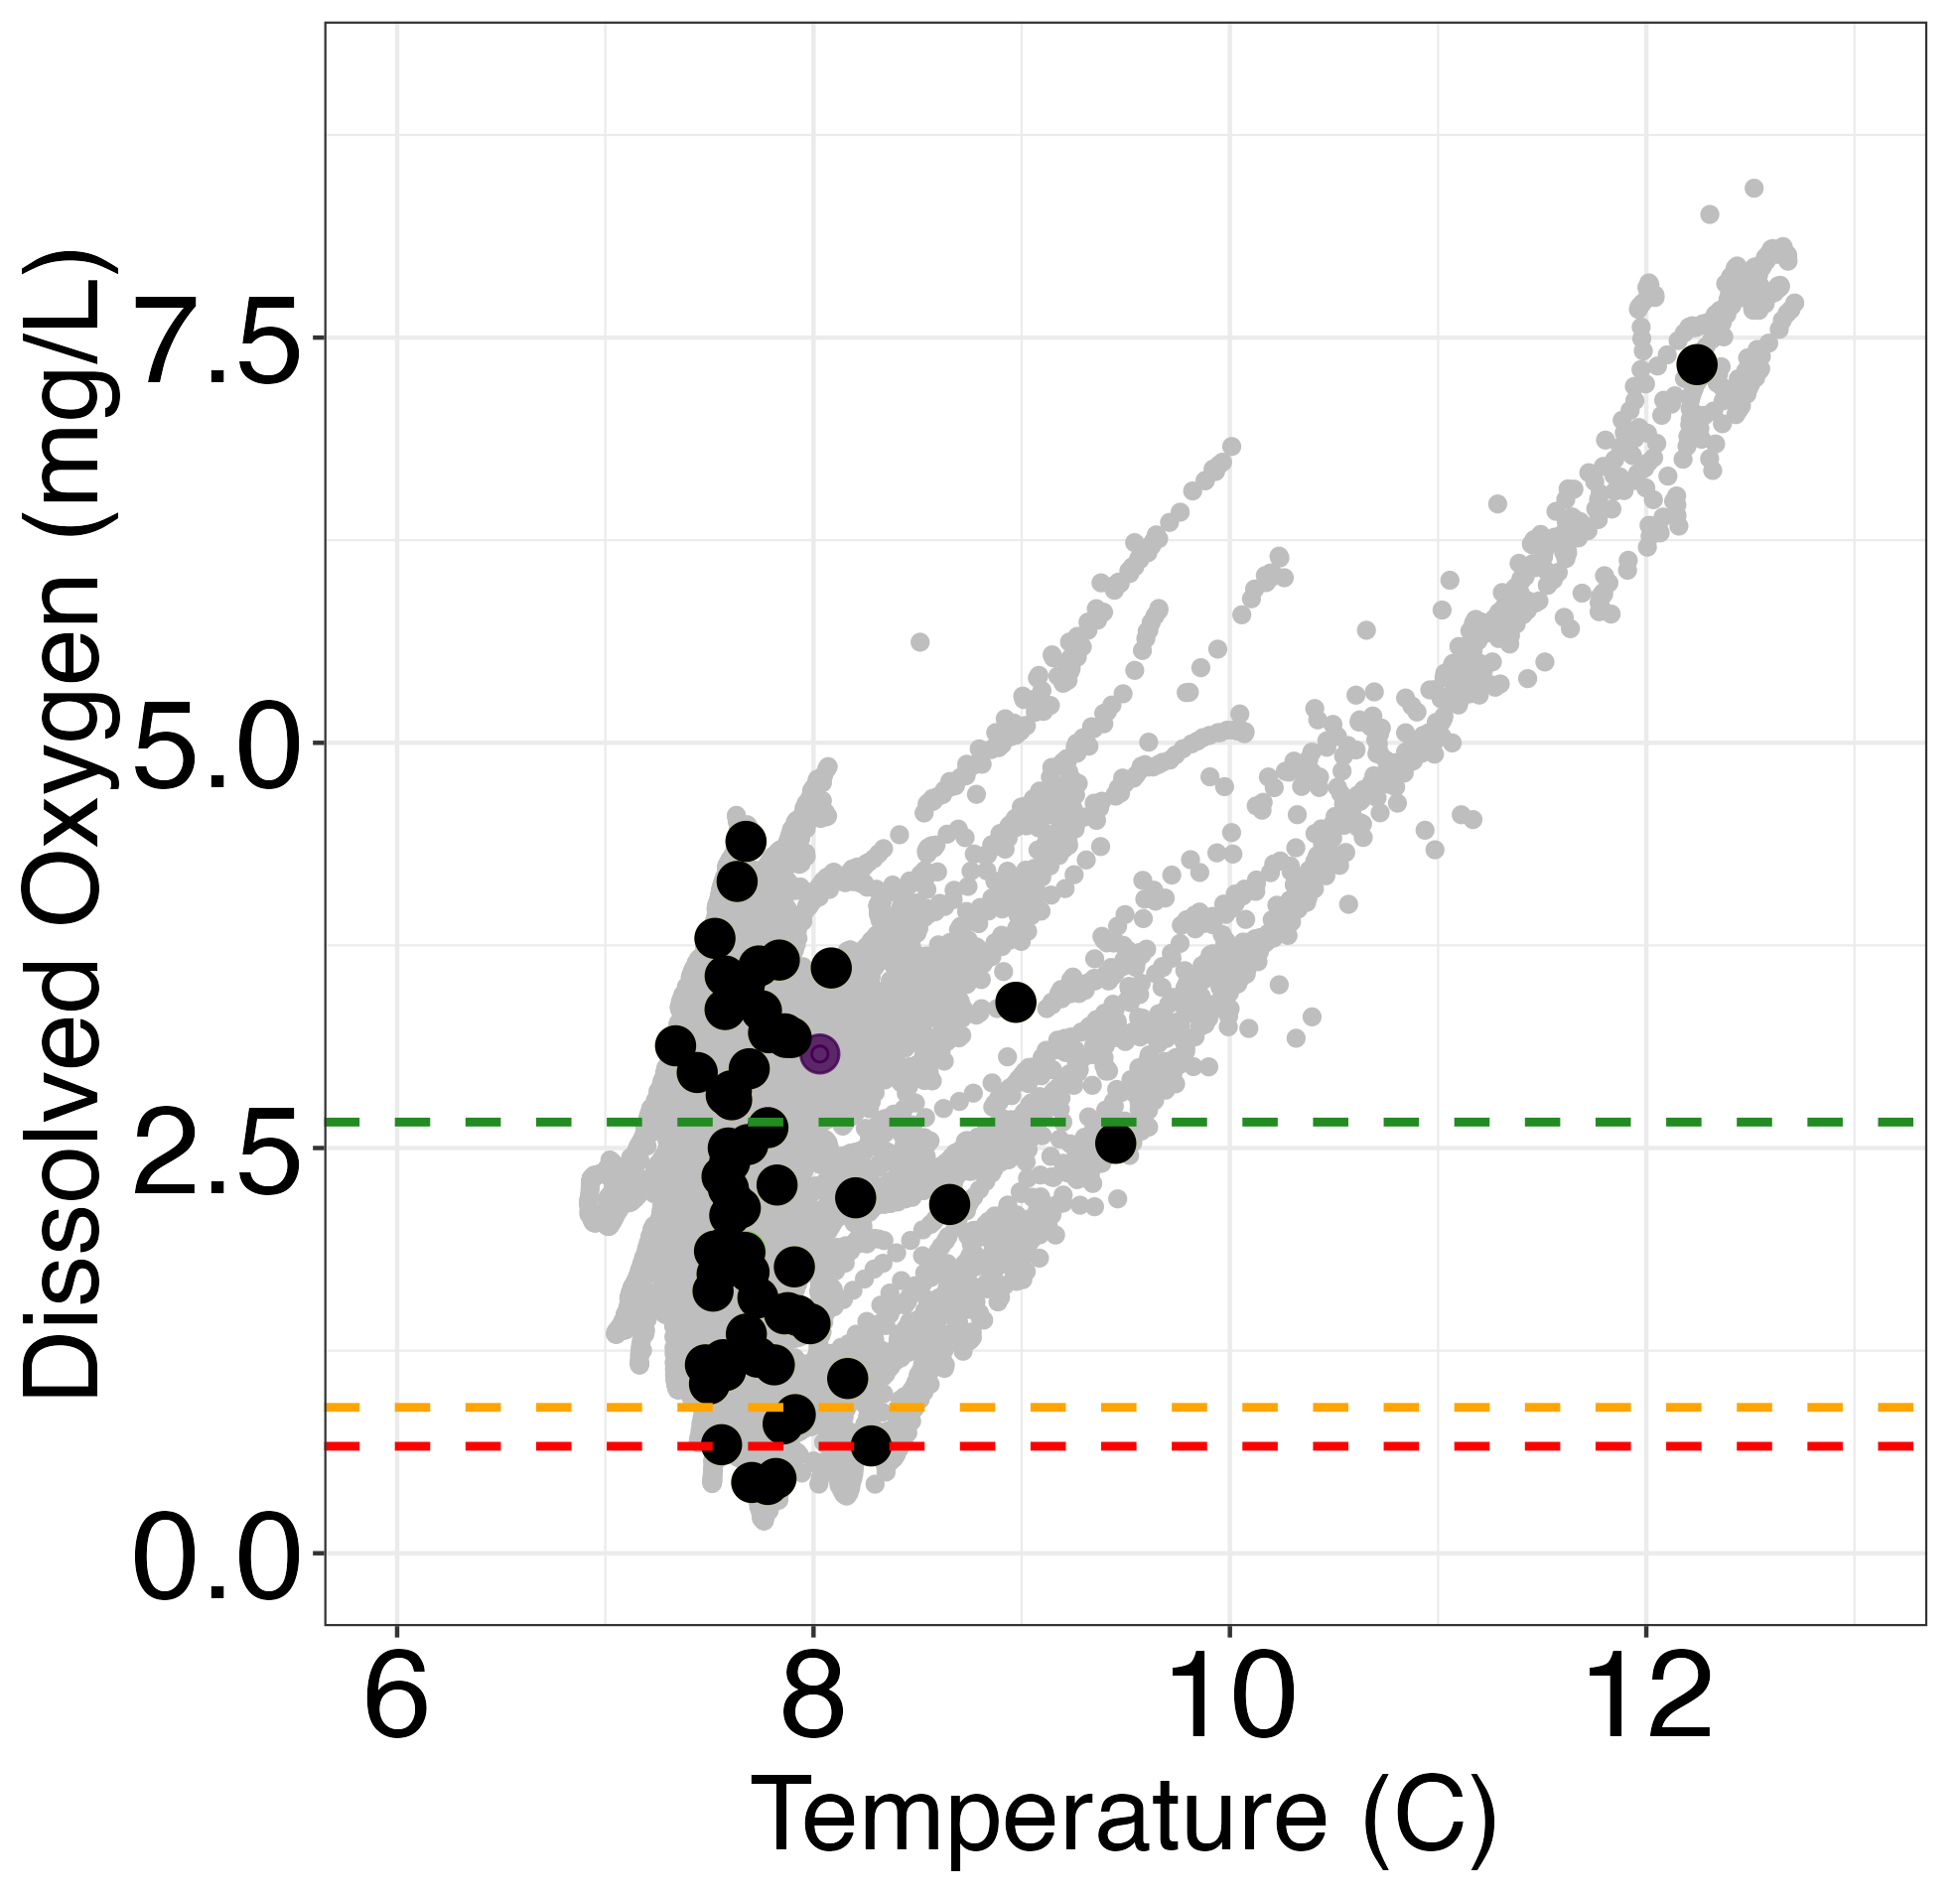
\includegraphics[scale=0.4]{Scatter_ex}
			b. \includegraphics[scale=0.4]{Scatter_ex_Mod}
			\caption[Mooring vs. Model Scatterplot]{Distribution of samples versus the distribution of temperature and dissolved oxygen during the entire sampling period, of May-October 2021-23. LiveOcean model output from winter months is not shown, since the eDNA sampler and TH042 mooring were not deployed during winter months. Gray dots indicate any environmental data sampling time, from the TH042 mooring (a) or from the LiveOcean model (b). Black dots indicate environmental conditions at which eDNA samples were taken. Note the high outliers, which are during a short heatwave in September 2021 and will not be shown in future scatterplots or considered in statistical analyses due to their small sample size.} \label{EnvironmentalConditions}%the special ToC caption is in square brackets. The \footnotesize makes the figure caption smaller
		\end{center}
		
	\end{figure} 
	
	I attempted to generate zero-inflated beta regression models using the zoib R package, but due to difficulties in visualizing the model output I switched to the brms package, a more general modeling package that uses Stan \autocite{Burkner2024}. I chose a zero-inflated beta regression because eDNA index ranges from zero to one, necessitating a beta regression, and the data is zero-inflated because each species was absent from many samples. I used the output of these models to generate and plot mean predicted data. I then compared these models to the binomial regression models, which related the presence and absence of eDNA to dissolved oxygen. Based on the Akaike information criterion (AIC), the binomial regression models performed better (lower AIC) for \textit{A. longiremis, C. pacificus, O. similis, Paracalanus sp. C AC-2013, P. mimus,} and \textit{P. newmani}. Based on AIC again, the zero-inflated beta regression models performed better for \textit{C. parapergens, Lucicutia flavicornis, Metridia lucens, M. pacifica,} and \textit{P. acuspes}. The zero-inflated beta regression for \textit{C. pacificus} performed better with the mooring data, but the binomial regression model for \textit{C. pacificus} performed better with the modeled data. Overall, in species with 5 or fewer detections, the binomial regression models performed better, but in species with more than 5 detections, the zero-inflated beta regression models performed better. I considered there to be a significant response for a species to hypoxia using binomial regression based on alpha = 0.05, and I considered zero-inflated beta regressions to be significant if their 95\% confidence interval showed an upward trend and did not include zero for every DO value (e.g. the 95\% confidence interval left the x-axis at any point, see Appendix \ref{chap:appZOIB} for visualized model confidence intervals). I did not perform significance tests directly comparing size categories or northern and southern copepods in aggregate, because the number of species with more than 5 detections was too low. 

	% missing here is a discussion of how you infer statistical significance once obtaining the right model. For both beta and binomial regression, you need to say how you are doing this, and what alpha value you are using. if you are using CIs that don't overlap the same place across the range of DO values, that's fine too
	% i'd end with a sentence that says that you dont significance test the N vs S or size range categories b/c you have low sample size after removing rare taxa

	\chapter{Results}
	
	%   p (Page) Place the table at the top of the next page. 
	% b (Bottom) Place the table at the bottom of the current page.
	% h (Here) Place the table at the spot where the table environment appears in the text
	% t (Top) Place the table at the top of the current page.
	% ! No seriously, put it where I told you to
	
	After bioinformatics and quality filtering, the total number of reads from the CO1 primer was 2,454,571, with 611,924 from copepods. From the CO1 primer reads, 569 unique species were identified, of which 16 were copepods with useable DNA reads in the dataset. The highest number of reads in one sample was 62,940, and the highest number of copepod reads in a sample was 19,335. The copepod eDNA detections dataset contained 26 samples from 2021, 35 samples from 2022, and 26 samples from 2023. In total, there were 556,748 DNA reads from copepods detected more than once during the study period, 364,980 of which were from 2021 and 2022. 
	
	Of the copepod species detected in the data, 5 species had more than 10 detections: \textit{A. longiremis, P. mimus, Paracalanus} sp. C AC-2013, \textit{P. newmani}, and \textit{O. similis}. \textit{C. abdominales} had 7 detections overall, with one in 2023. \textit{C. pacificus} had 5 detections, none of which were in 2023, and \textit{P. acuspes} had 5 detections, 2 of which were in 2023. All other copepod species had fewer than 5 detections overall.
	
	
	%Then the abundance - and highlight if/where there are differences. I would also have a summary table for the species detected that is color coded to spell out the northern versus southern expectations versus observations. You could have a column of species, a column of northern versus southern, a column of observed occurrence/prevalence results, and a column of observed abundance results. Blue for cold and red for warm and then you could see how well that lined up
	
%	\begin{center} 
%		\begin{tabular}{l | l | l l | l l}  
%			\toprule
%			Species & Group & Prevalence & Abundance}
%			\midrule
%			\textit{Acartia longiremis}	& Cold-water & pos & neg \\
%			\bottomrule 
%		\end{tabular}
%		\label{ZOIBtab}
%	\end{center}
%	\end{table}
	
	%Northern vs southern eDNA oxygen
	
	\section{Dissolved Oxygen and Species Abundance}  
	
	Most of the northern copepods studied had higher eDNA index at higher dissolved oxygen levels, with a positive correlation between eDNA index and DO according to zero-inflated beta regressions (See Appendix \ref{chap:appZOIB}). All northern copepods except \textit{P. newmani} were more abundant at higher dissolved oxygen levels according to zero-inflated beta regressions based on the TH042 mooring data from 2021-22 (See Table \ref{ZOIBtab}). Of these northern copepods, \textit{A. longiremis} and \textit{P. mimus} had significant positive correlations between eDNA and DO. 
	
	\begin{table}[!h] 
			\begin{tabular}{l | l | l l | l l}
				\toprule
				Species & Group & \multicolumn{2}{|c|}{Detections} & \multicolumn{2}{|c}{Regression Results} \tabularnewline
				\midrule
				Species &  Group & 2021-22 & 2021-23 & 2021-22 & 2021-23  \\ 
				\midrule 
				\textcolor{RoyalBlue}{\textit{Acartia longiremis}}	& Cold-water & 61 & 86 & \textcolor{ForestGreen}{Positive*} & Neutral  \\
				\textcolor{RoyalBlue}{\textit{Pseudocalanus mimus}} & Cold-water & 28  & 46 & \textcolor{ForestGreen}{Positive*} & \textcolor{BrickRed}{Negative*}  \\
				\textcolor{RoyalBlue}{\textit{Pseudocalanus newmani}}	& Cold-water & 20  & 25 & Neutral & Neutral* \\
				\textcolor{RoyalBlue}{\textit{Centropages abdominales}} & Cold-water & 6 & 7 & \textcolor{ForestGreen}{Positive} & Neutral   \\
				\textcolor{RoyalBlue}{\textit{Pseudocalanus acuspes}}  & Cold-water & 3  & 5 & \textcolor{ForestGreen}{Positive} & Neutral  \\
				\textit{Oithona similis} & Year-round & 11  & 11 & Negative* & Neutral \\
				\textcolor{RedOrange}{\textit{Paracalanus} sp. C. AC-2013} & Warm-water & 33  & 33 & Neutral & \textcolor{ForestGreen}{Positive*}  \\
				\textcolor{RedOrange}{\textit{Calanus pacificus}}	& Warm-water & 5  & 5 & \textcolor{BrickRed}{Negative} & \textcolor{BrickRed}{Negative}  \\
				\bottomrule 
			\end{tabular}
			
			\caption[Zero-inflated beta regression results]{Trends of zero-inflated beta regressions relating dissolved oxygen concentration to eDNA index for different species of copepods. Regressions were computed using the TH042 mooring data from 2021-22, and again using LiveOcean model data from 2021-23, so both are shown. I considered trends to be significant (marked with ``*" in this table) if their 95\% confidence interval showed an upward trend and did not contain zero at some DO value. See Appendix \ref{chap:appZOIB} for plotted regression results. Cold-water copepods (blue) are northern copepods, warm-water copepods (orange) are southern.}  \label{ZOIBtab}
	\end{table}
	
	\section{Dissolved Oxygen and Species Prevalence} 
	
	The data suggests that northern copepods have a comparatively lower tolerance to hypoxia. Southern copepods and \textit{O. similis}, which is present year-round, were detected proportionally more at dissolved oxygen levels below 0.9 mg/L (see Figure \ref{BarSeason}a). However, the northern copepod \textit{P. newmani} had fewer detections at high dissolved oxygen levels according to a binomial regression comparing LiveOcean modeled DO to species presence, but the effect was not significant (-0.30, df = 2, 89, 2, p = 0.36). \textit{P. newmani} did have significantly fewer detections at high dissolved oxygen levels when the binomial regresion was calculated using the TH042 mooring data for all three years (-0.64, df = 2, 63, 2, p = 0.03), see Figure \ref{PnewmaniBinomDensity}). \textit{P. newmani} also had a relatively consistent eDNA index across DO levels according to a zero-inflated beta regression, so while its prevalence was higher in hypoxic conditions, its abundance was not (See Appendix \ref{chap:appZOIB}). 
	
	\begin{figure}[!h]
		\begin{center}
			a. 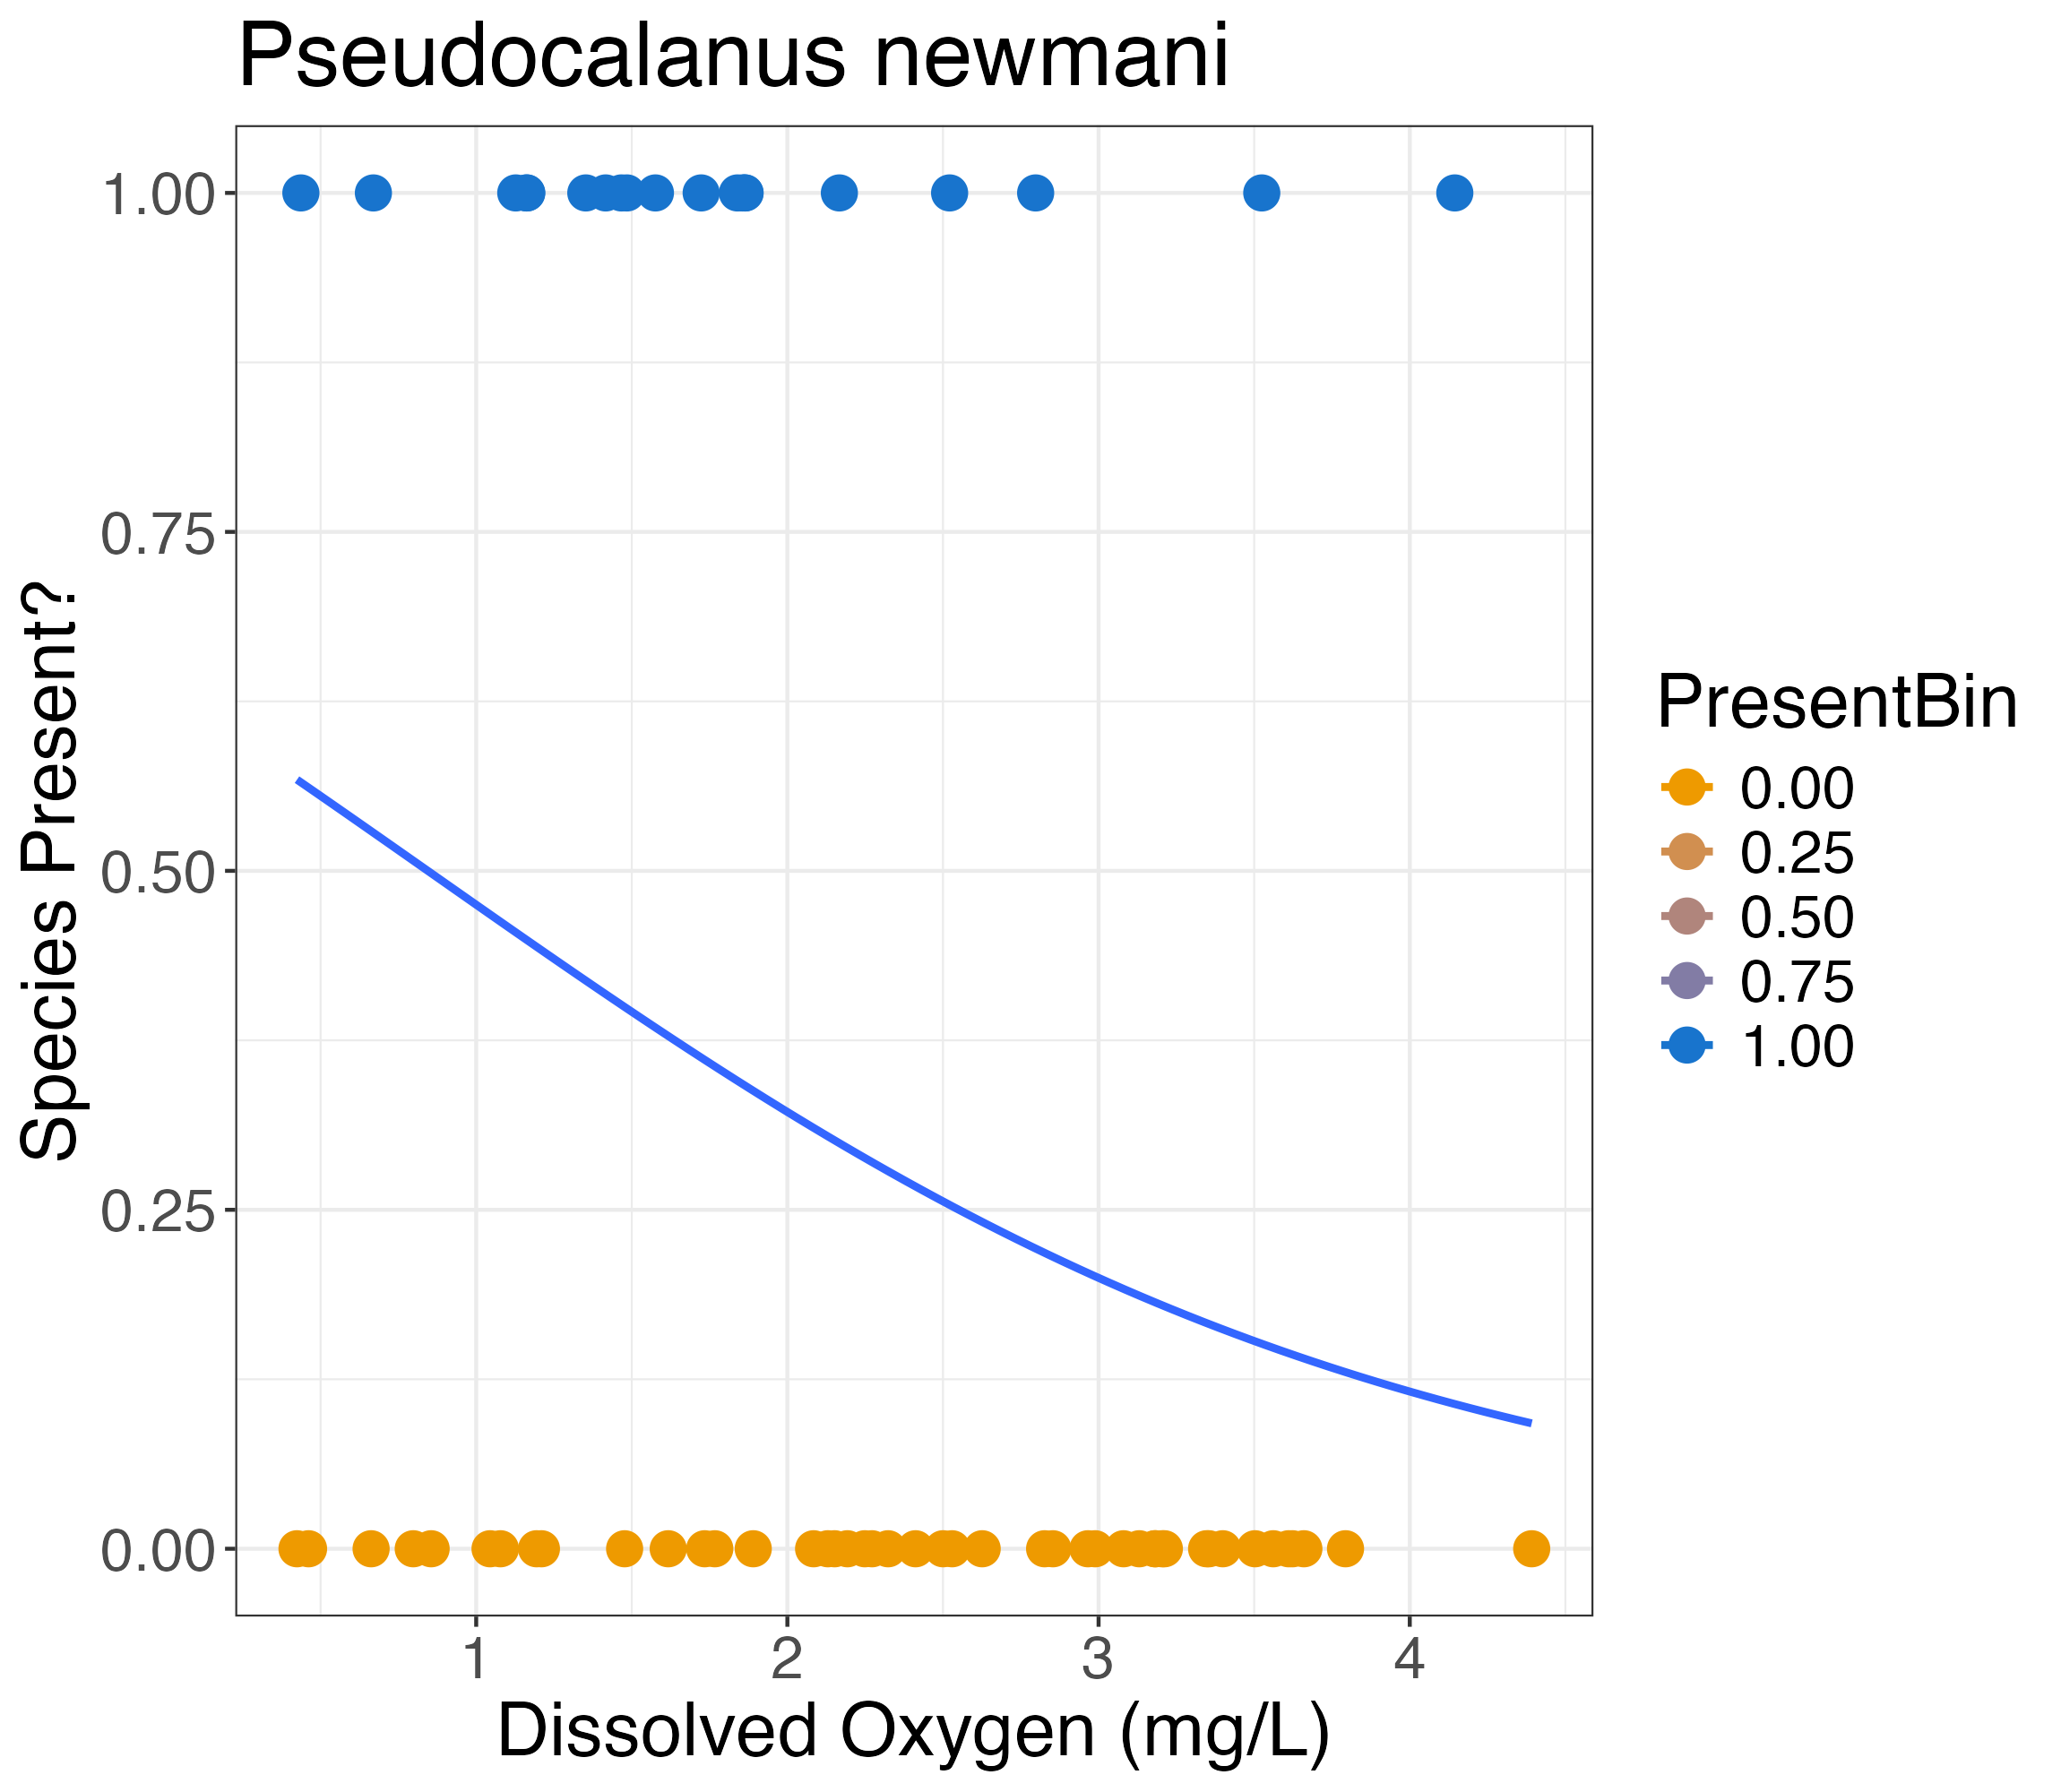
\includegraphics[scale=0.3]{Pnewmani_binom_sig_neg}
			b. 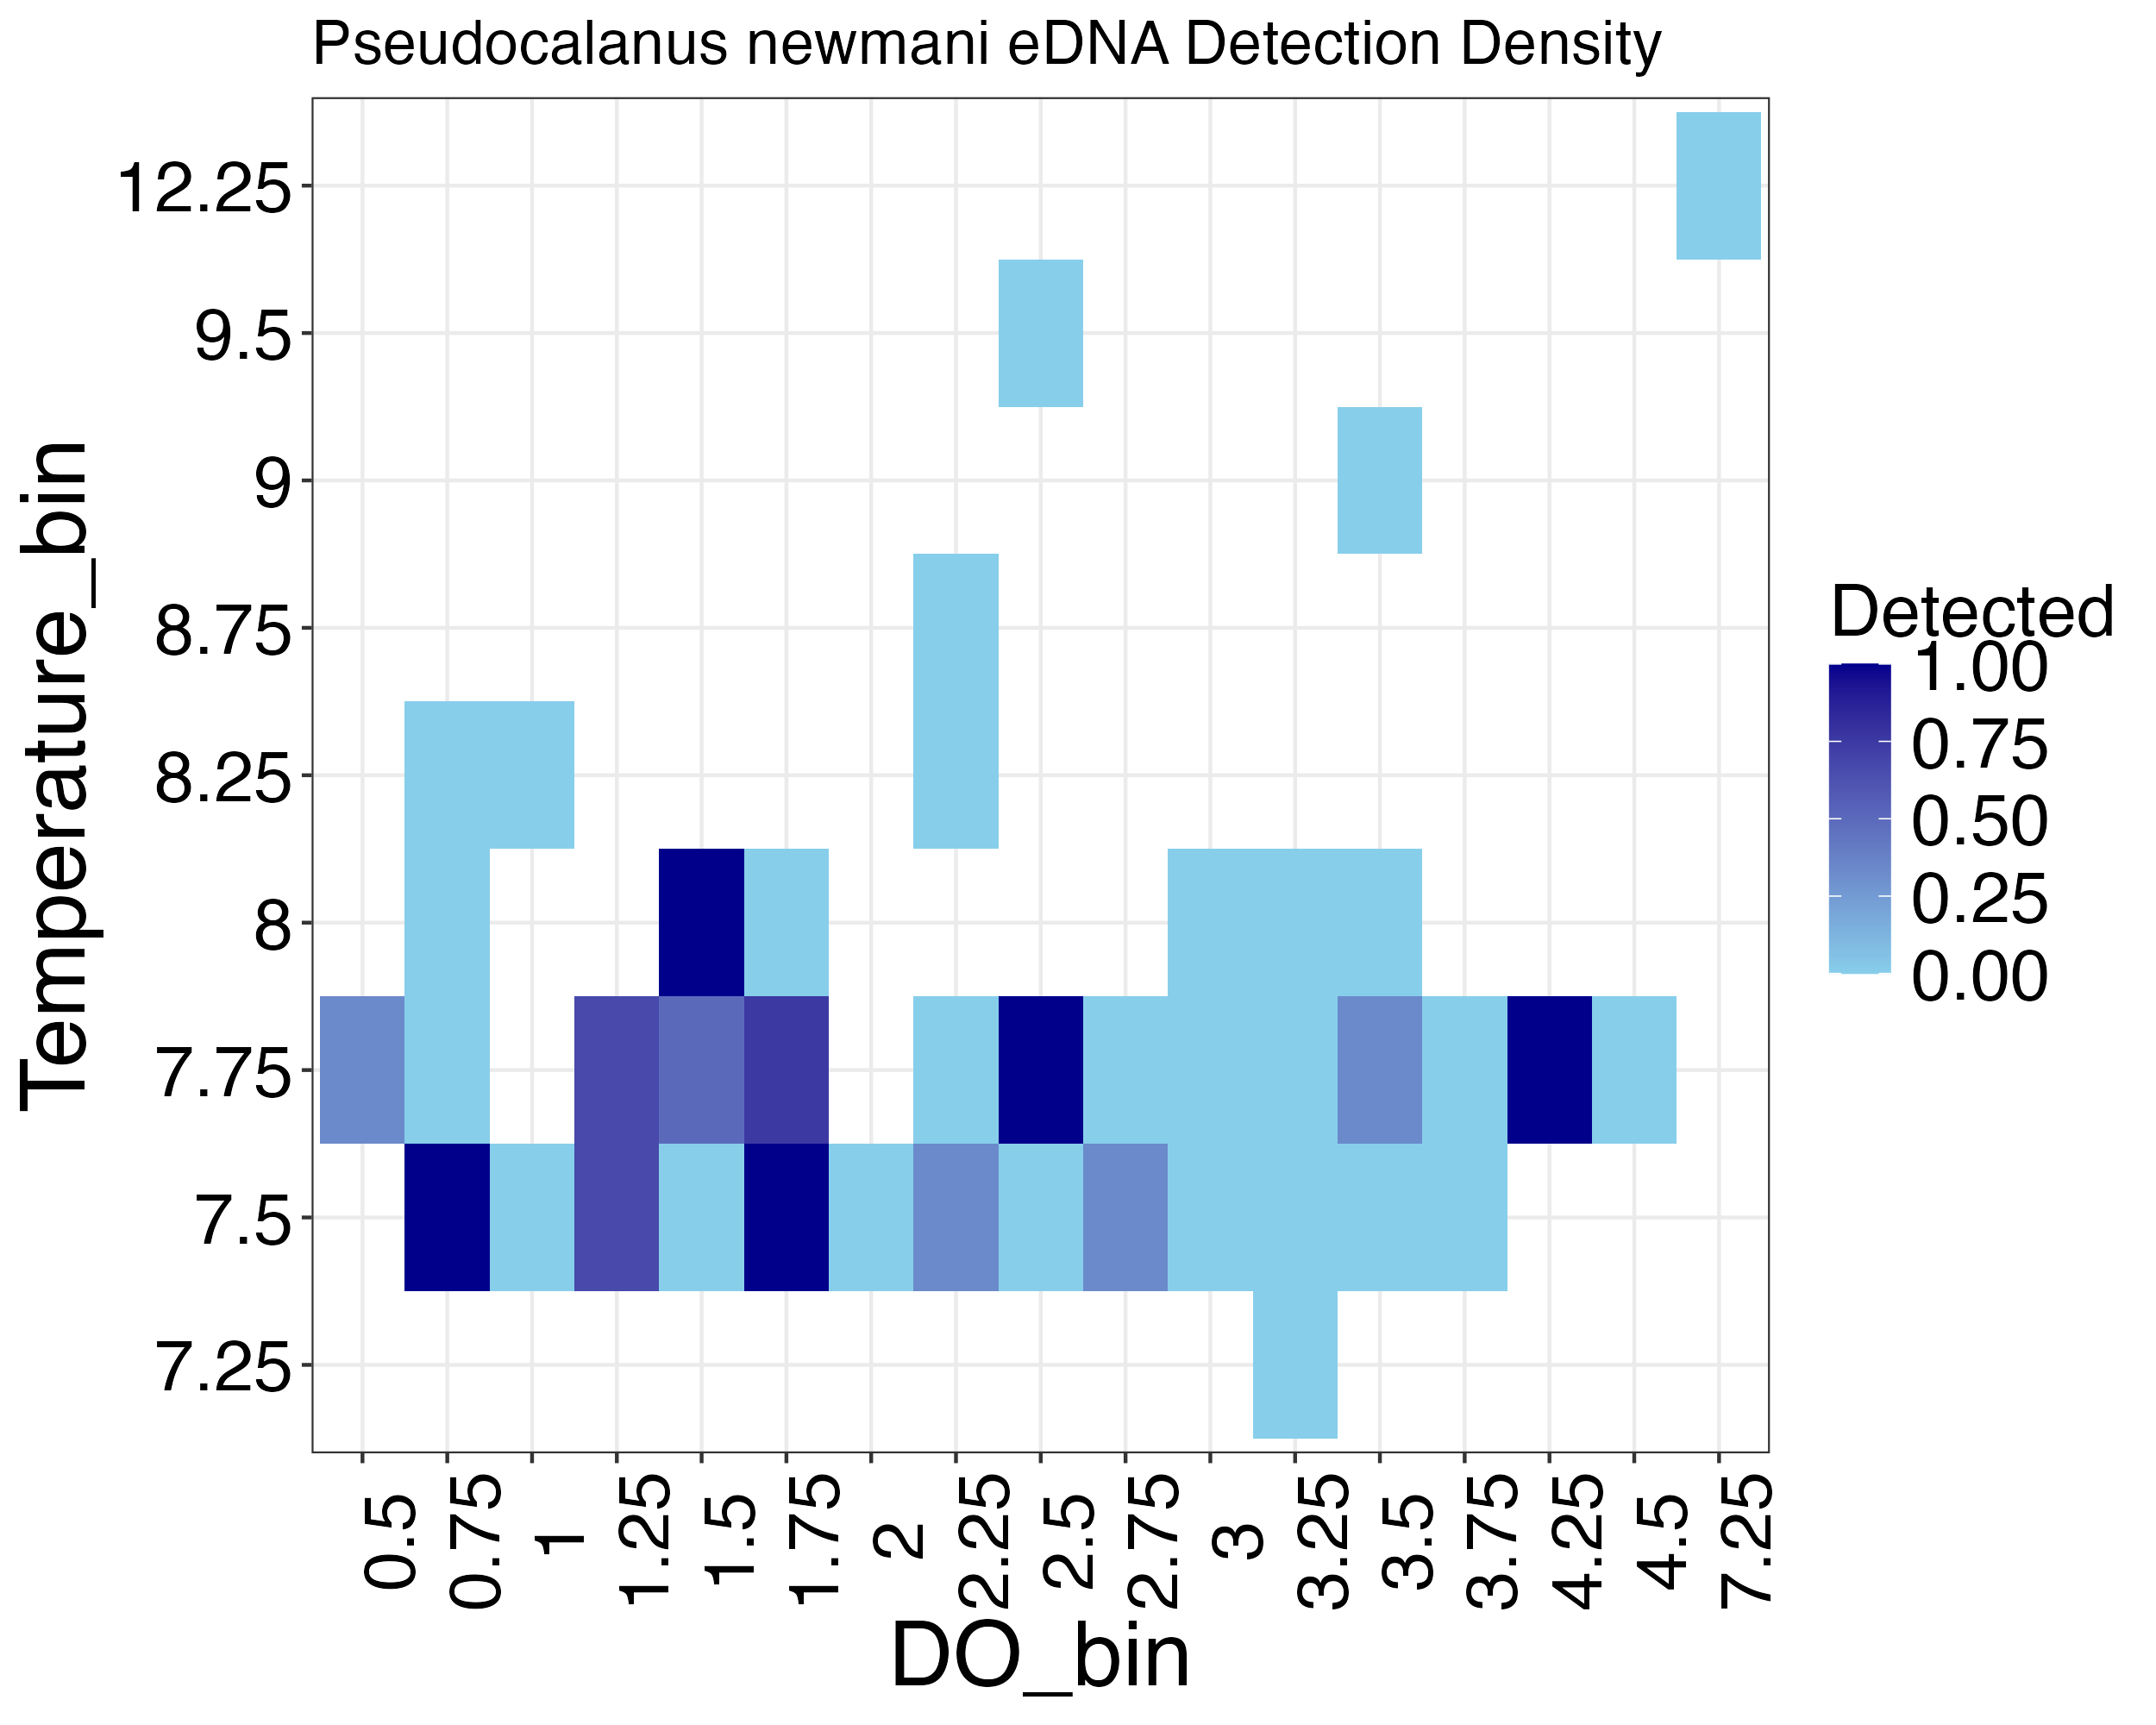
\includegraphics[scale=0.3]{Pnewmani_Density} \\
			\caption[\textit{P. newmani} binomial regression and density plot]{\footnotesize{Dissolved oxygen data from the TH042 mooring in 2021-22 compared to \textit{P. newmani} detections. (a) \textit{P. newmani} binomial regression comparing species presence to dissolved oxygen. \textit{P. newmani} was detected significantly less frequently at higher dissolved oxygen levels. (b) Density plot of \textit{P. newmani} detections. Each pixel represents a range of dissolved oxygen and temperature values, and the shade of each pixel represents the proportion of eDNA samples in that environmental range in which \textit{P. newmani} was detected. \textit{P. newmani} was primarily detected below 2.5 mg/L DO.}} %the special ToC caption is in square brackets. The \footnotesize makes the figure caption smaller
			\label{PnewmaniBinomDensity}
		\end{center}
	\end{figure} 
	
	\begin{figure}[!h]
		\begin{center}
			a. 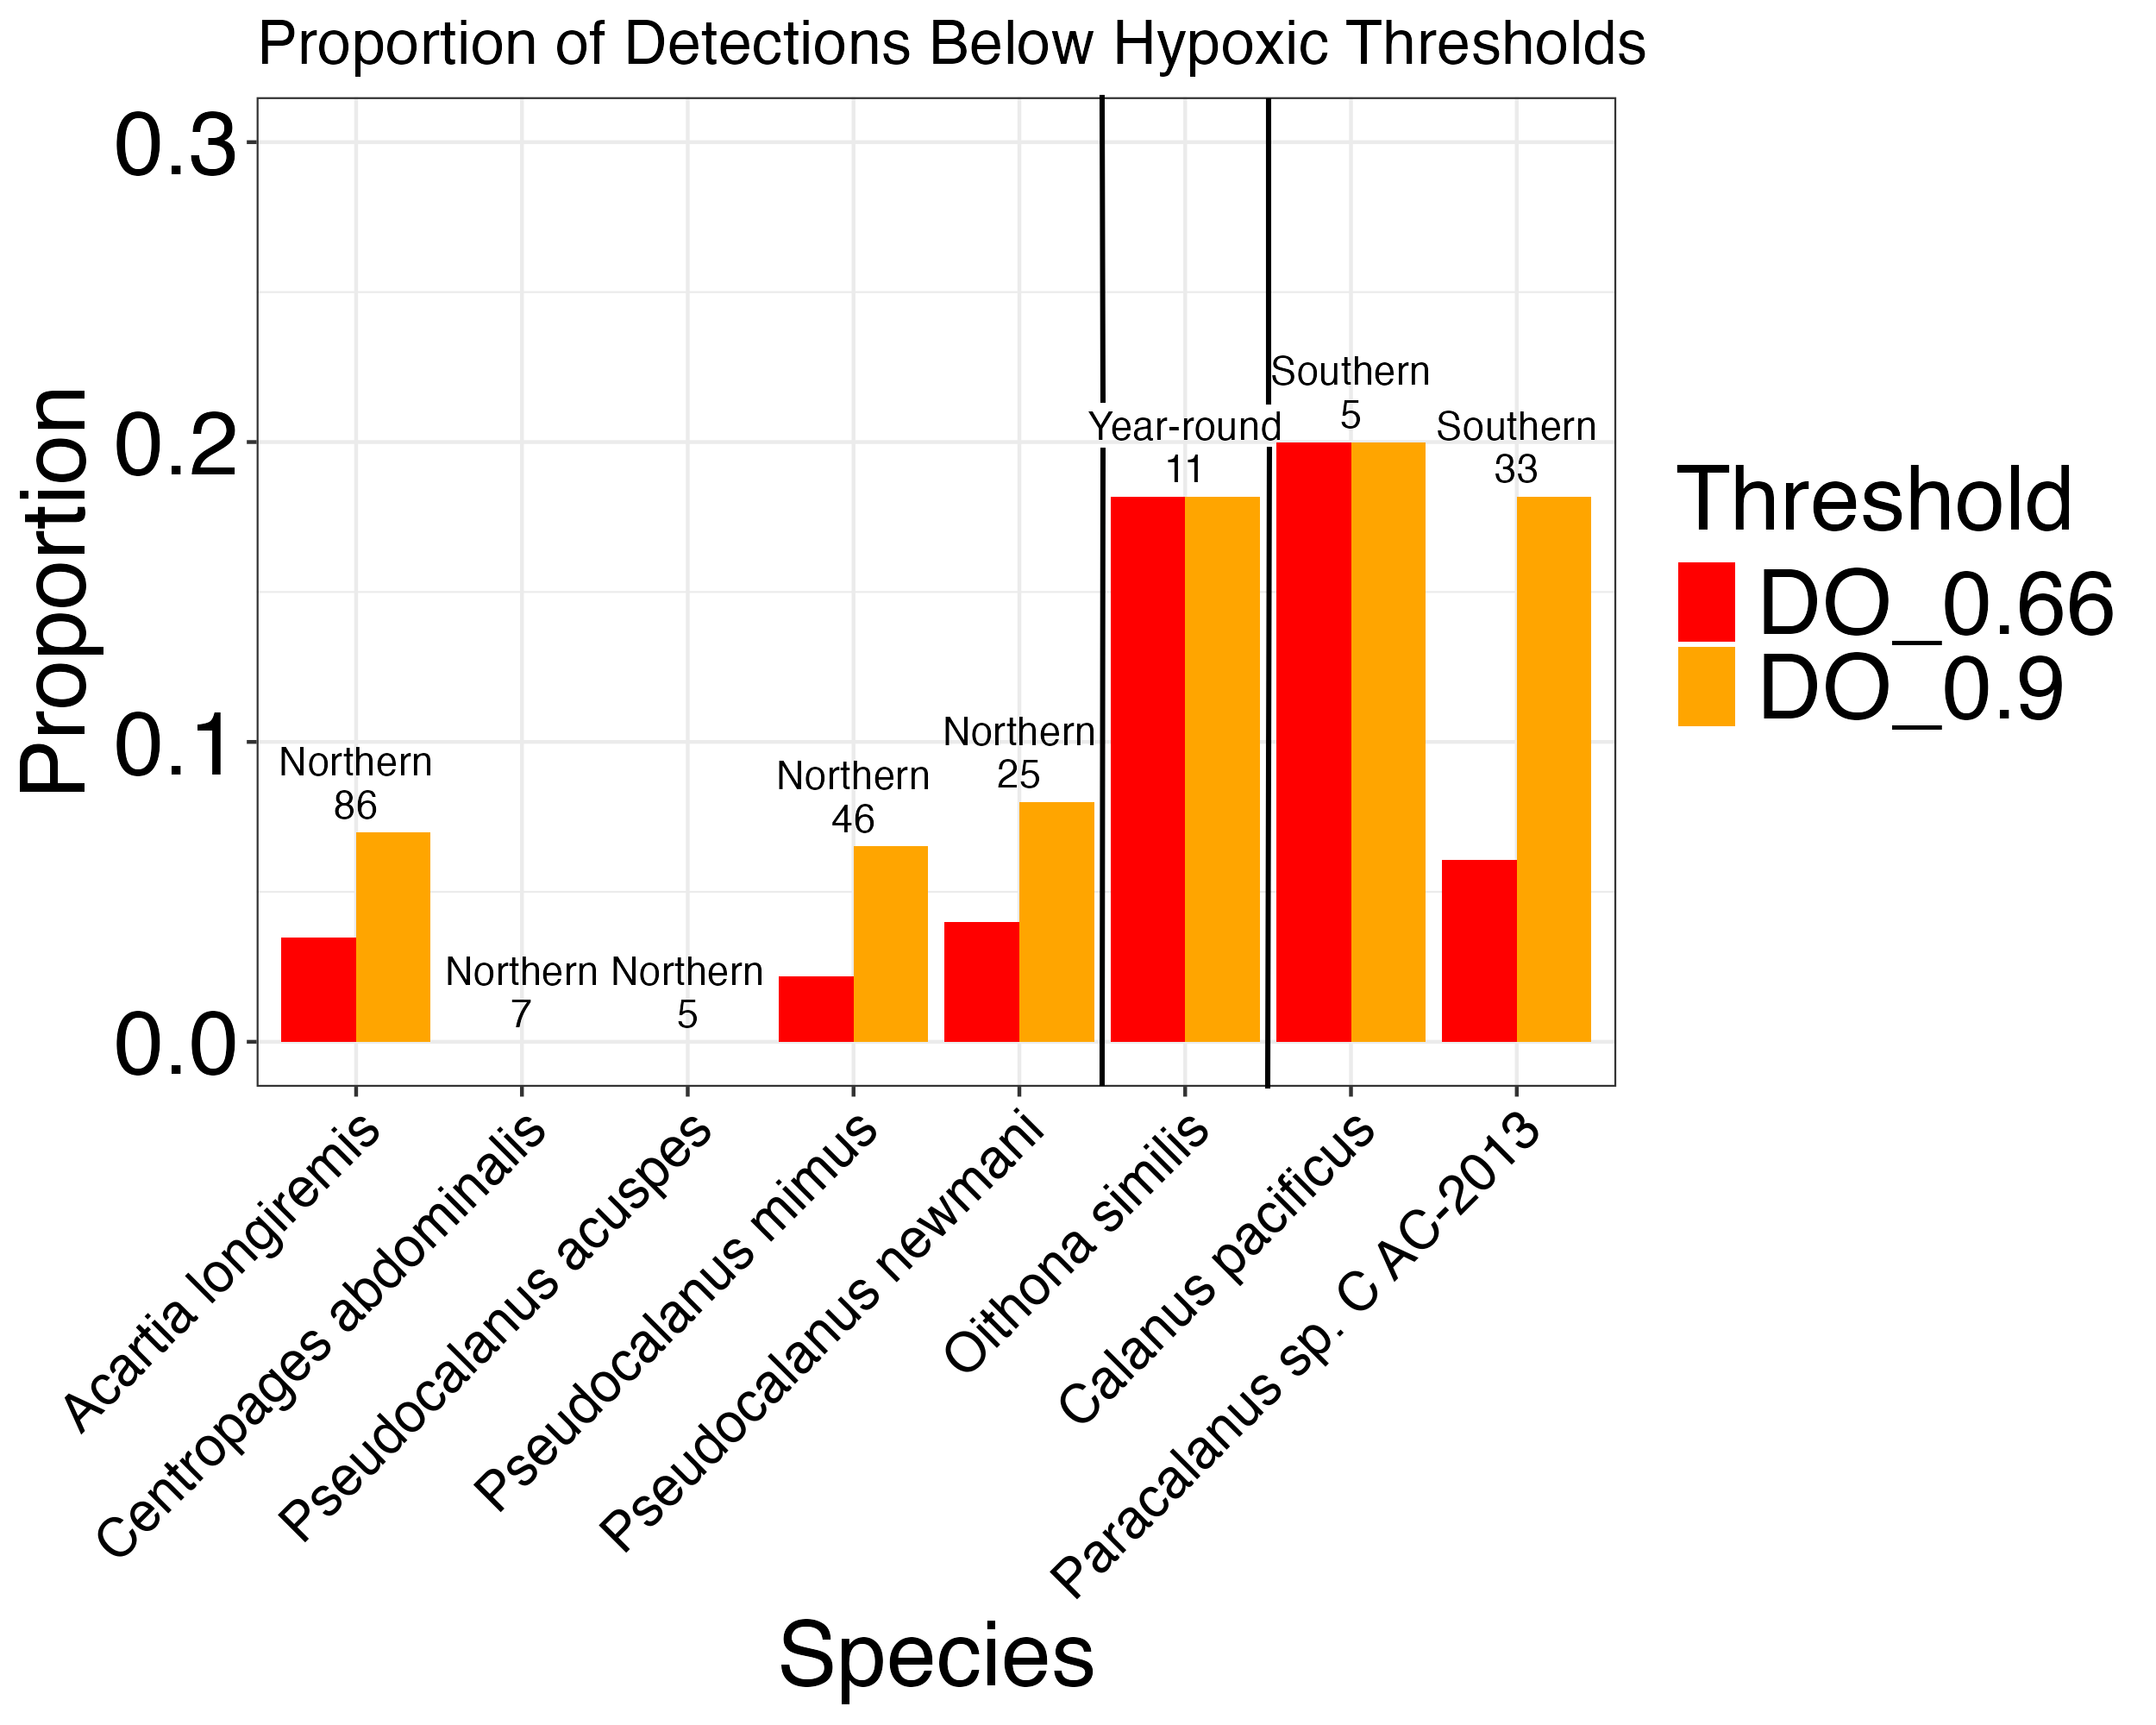
\includegraphics[scale=0.5]{Bar_Season} \\
			b. 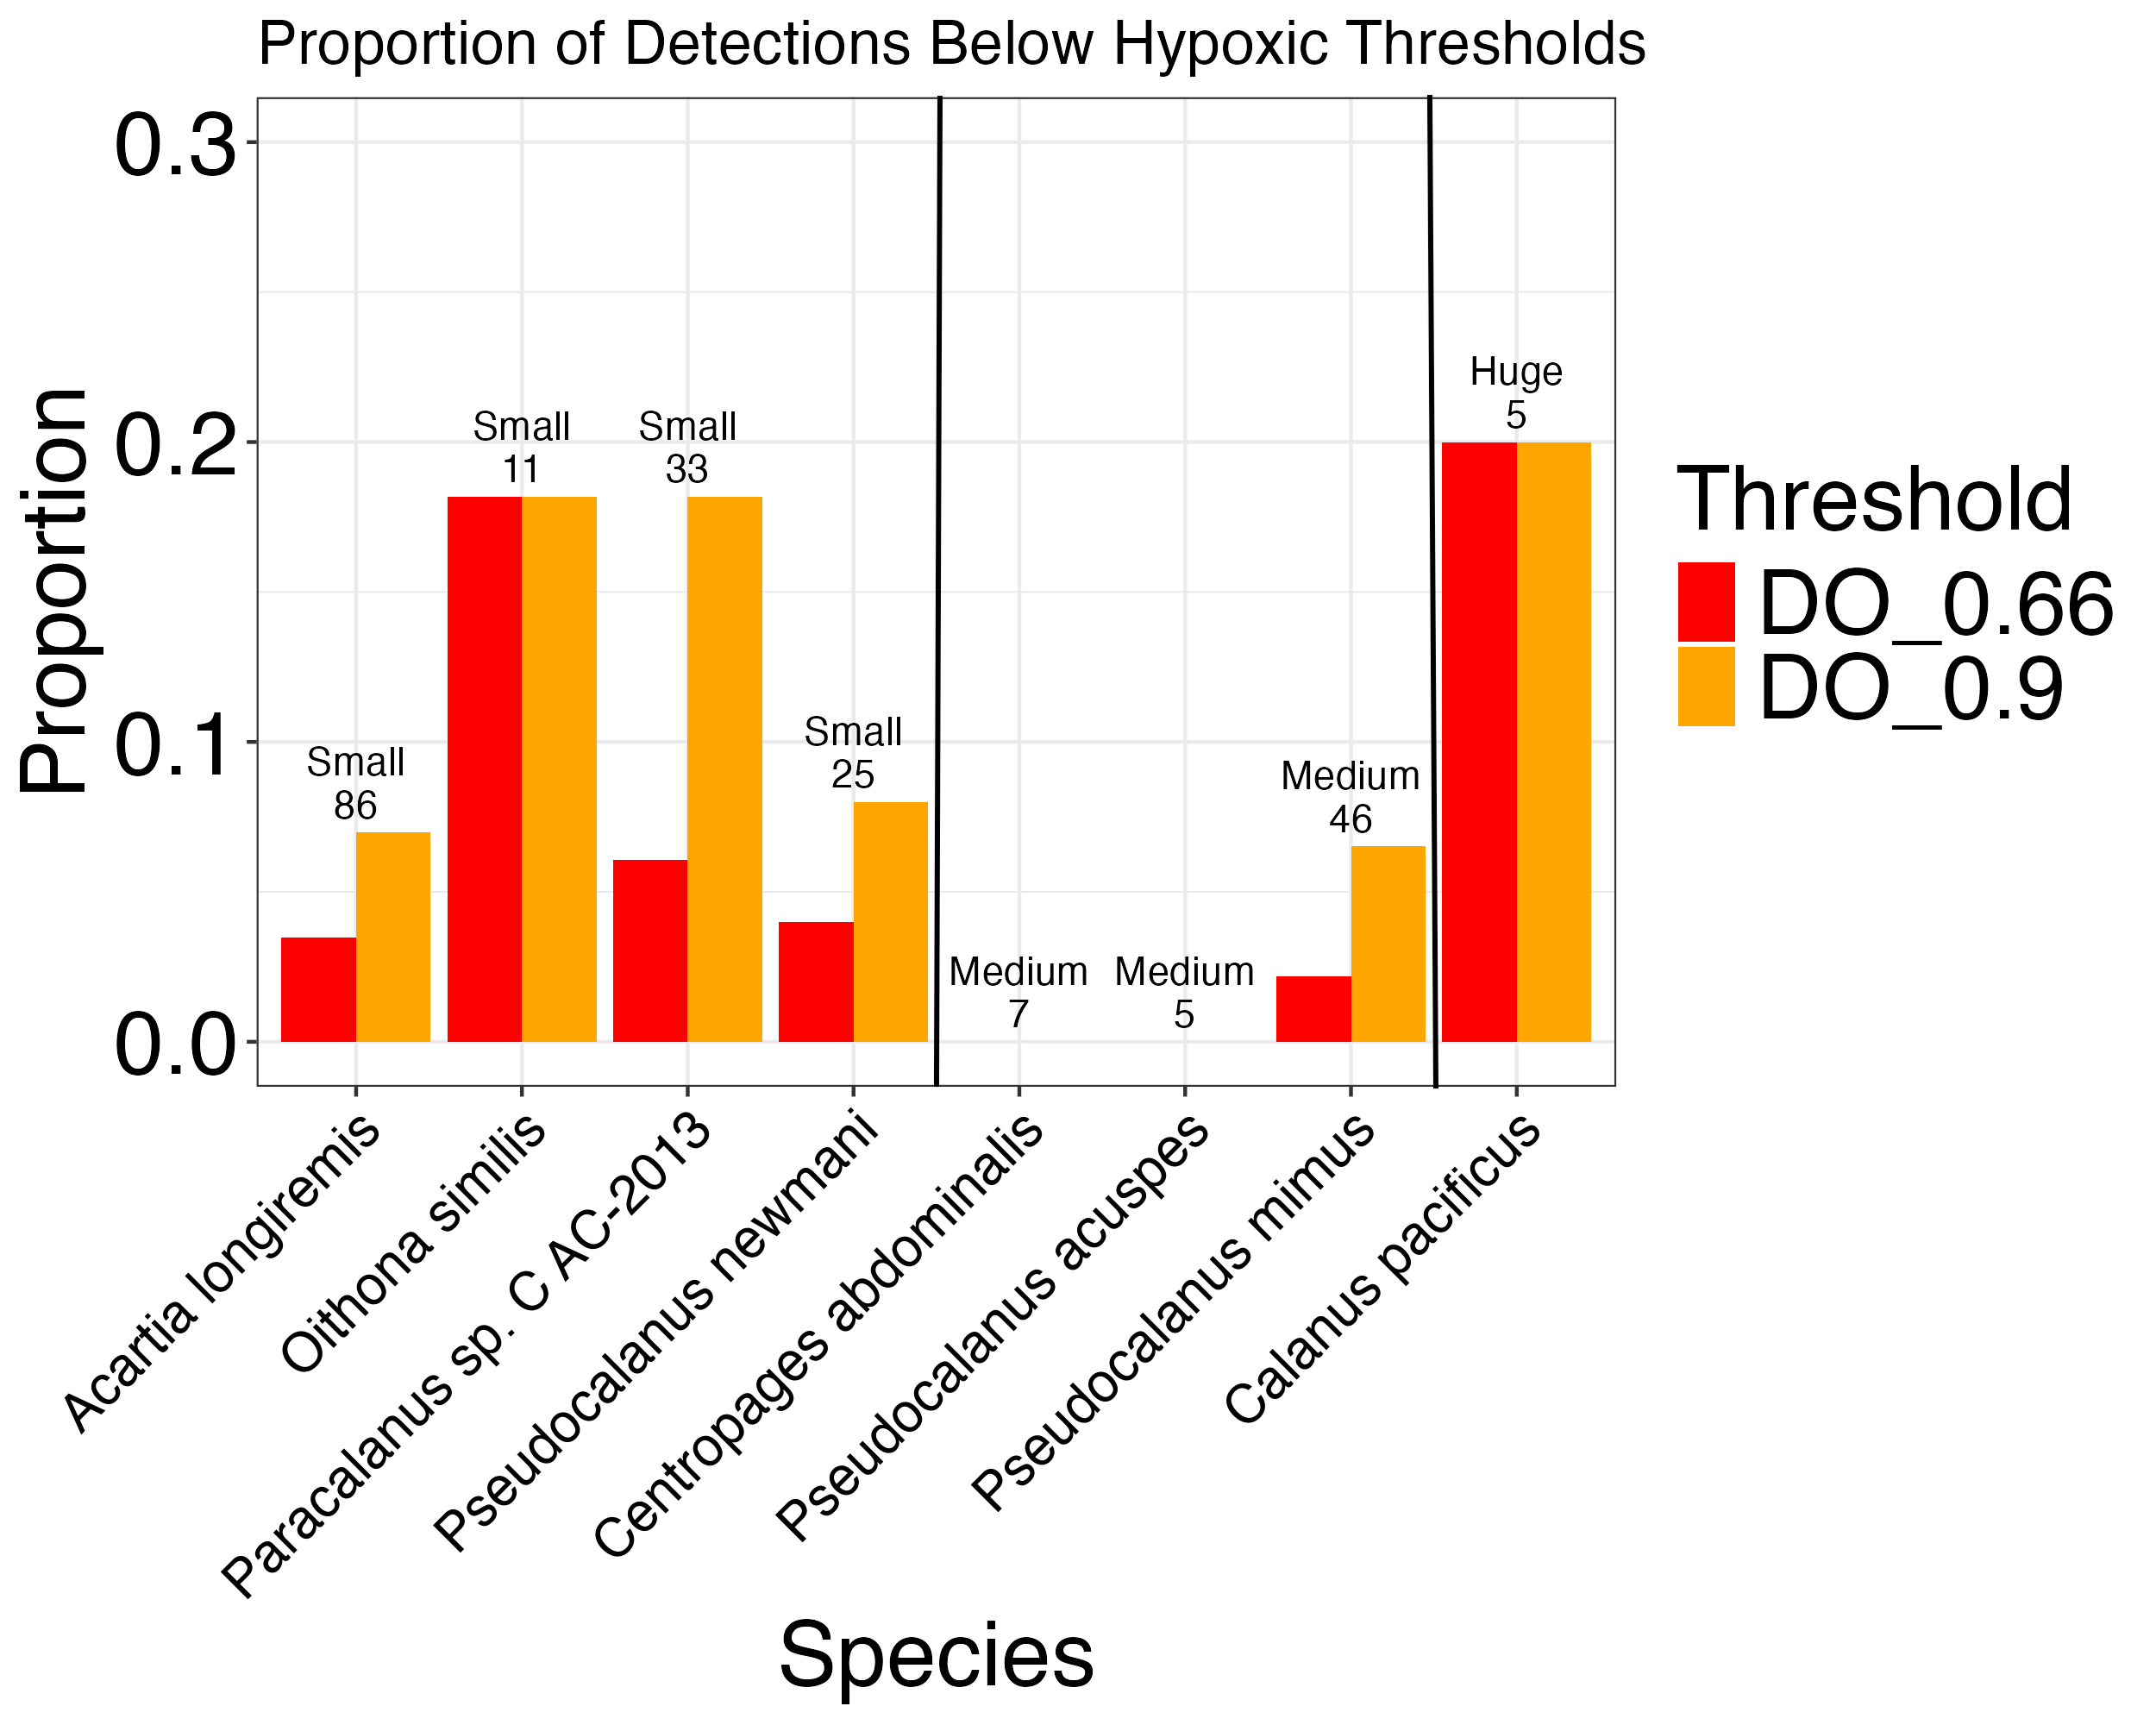
\includegraphics[scale=0.5]{Bar_Size}
			\caption[Proportion of Detections Below Hypoxic Thresholds]{\footnotesize{A comparison of different copepod groups and their rates of occurence below certain hypoxic thresholds. Red bars indicate the proportion of detections of that species that were in conditions below 0.66 mg/L of oxygen, and orange bars indicate the proportion of detections of that species that were in conditions below 0.9 mg/L of oxygen. Numbers above bars are the total number of detections of that species. In plot (a) copepods are labeled by seasonal groupings. In plot (b), copepods are labeled by size category. Species with a maximum size of less than 1.5 mm are Small, maximum size 1.5-2.5 mm is Medium, maximum size 2.5-4 mm is Large, and maximum size ${>}$4 mm is Huge \autocite{WoRMSWorldRegister}}} %the special ToC caption is in square brackets. The \footnotesize makes the figure caption smaller
			\label{BarSeason}
		\end{center}
	\end{figure}    
	
	% Species, north/south color coded, model results (binomial coefficient and p-value), directionality (color-coded)
	\begin{table}[!h] 
		\begin{tabular}{l | l | l l | l}
			\toprule
			Species & Group & \multicolumn{2}{|c|}{Binomial Regression} & Beta Regression \tabularnewline
			\midrule
			Species &  Group & Coefficient & P-value & (LiveOcean Data)  \\ 
			\midrule 
			\textcolor{RoyalBlue}{\textit{Acartia longiremis}}	& Cold-water & -0.03 & 0.9 & Neutral  \\
			\textcolor{RoyalBlue}{\textit{Pseudocalanus mimus}} & Cold-water & 0.07  & 0.5 & \textcolor{BrickRed}{Negative*}  \\
			\textcolor{RoyalBlue}{\textit{Pseudocalanus newmani}}	& Cold-water & -0.3  & 0.3 &  Neutral* \\
			\textcolor{RoyalBlue}{\textit{Centropages abdominales}} & Cold-water & -0.005 & 0.9 & Neutral   \\
			\textcolor{RoyalBlue}{\textit{Pseudocalanus acuspes}}  & Cold-water & 1.48  & 0.2 & Neutral  \\
			\textit{Oithona similis} & Year-round & 0.68  & 0.4 & Neutral \\
			\textcolor{RedOrange}{\textit{Paracalanus} sp. C. AC-2013} & Warm-water & 0.6  & \textcolor{ForestGreen}{0.03} & \textcolor{ForestGreen}{Positive*}  \\
			\textcolor{RedOrange}{\textit{Calanus pacificus}}	& Warm-water & -0.15  & \textcolor{ForestGreen}{0.044} & \textcolor{BrickRed}{Negative}  \\
			\bottomrule 
		\end{tabular}
		
		\caption[Regression results]{Trends of binomial regressions relating dissolved oxygen concentration to species detections and zero-inflated beta regressions relating dissolved oxygen concentration to eDNA index for different species of copepods. Regressions were computed using LiveOcean model data from 2021-23. I considered trends to be significant (marked with ``*" in this table) if their 95\% confidence interval showed an upward trend and did not contain zero at some DO value. See Appendix \ref{chap:appZOIB} for plotted regression results. Cold-water copepods (blue) are northern copepods, warm-water copepods (orange) are southern.}  \label{Resultstab}
	\end{table}
	
	% Size 
	Small copepod species showed a higher hypoxia tolerance than large copepod species in this study. Large and huge copepods (\textit{C. pacificus} and \textit{M. pacifica}) were rarely detected below 0.9 mg/L DO, although \textit{C. pacificus}, the only huge (larger than 4 mm) copepod in the dataset, was detected once below 0.6 mg/L DO with a high eDNA index (see Appendix \ref{chap:appPlots}). Medium copepods were rarely detected below 0.9 mg/L DO compared to small copepods (See Figure \ref{BarSeason}b). Small copepods were frequently detected below 0.6 mg/L DO, especially \textit{A. longiremis} and \textit{Paracalanus} sp. (see Figure \ref{BarSeason}b). \textit{O. similis}, a small copepod, was present below 0.6 mg/L DO, but generally had a higher eDNA index at higher values of DO (see Appendix \ref{chap:appPlots}).
	
	
	\section{Temperature}
	%Temperatures
	
	During this study, northern copepods were generally detected at lower temperatures than southern copepods. Most of the northern copepods in this study were not detected at temperatures above 8 ºC, except for \textit{P. mimus}, which was detected above 8 ºC but was not detected at the highest temperature in the dataset, 12.2 ºC. Southern copepods were primarily detected above 7.5 ºC, and the southern copepod \textit{Paracalanus} sp. C AC-2013 had higher eDNA index values measured above 8 ºC, despite being detected many times below 8 ºC (see Figure \ref{ParacalanusScatter}). 
	
	
	\begin{figure}[!h]
		\begin{center}
			a. 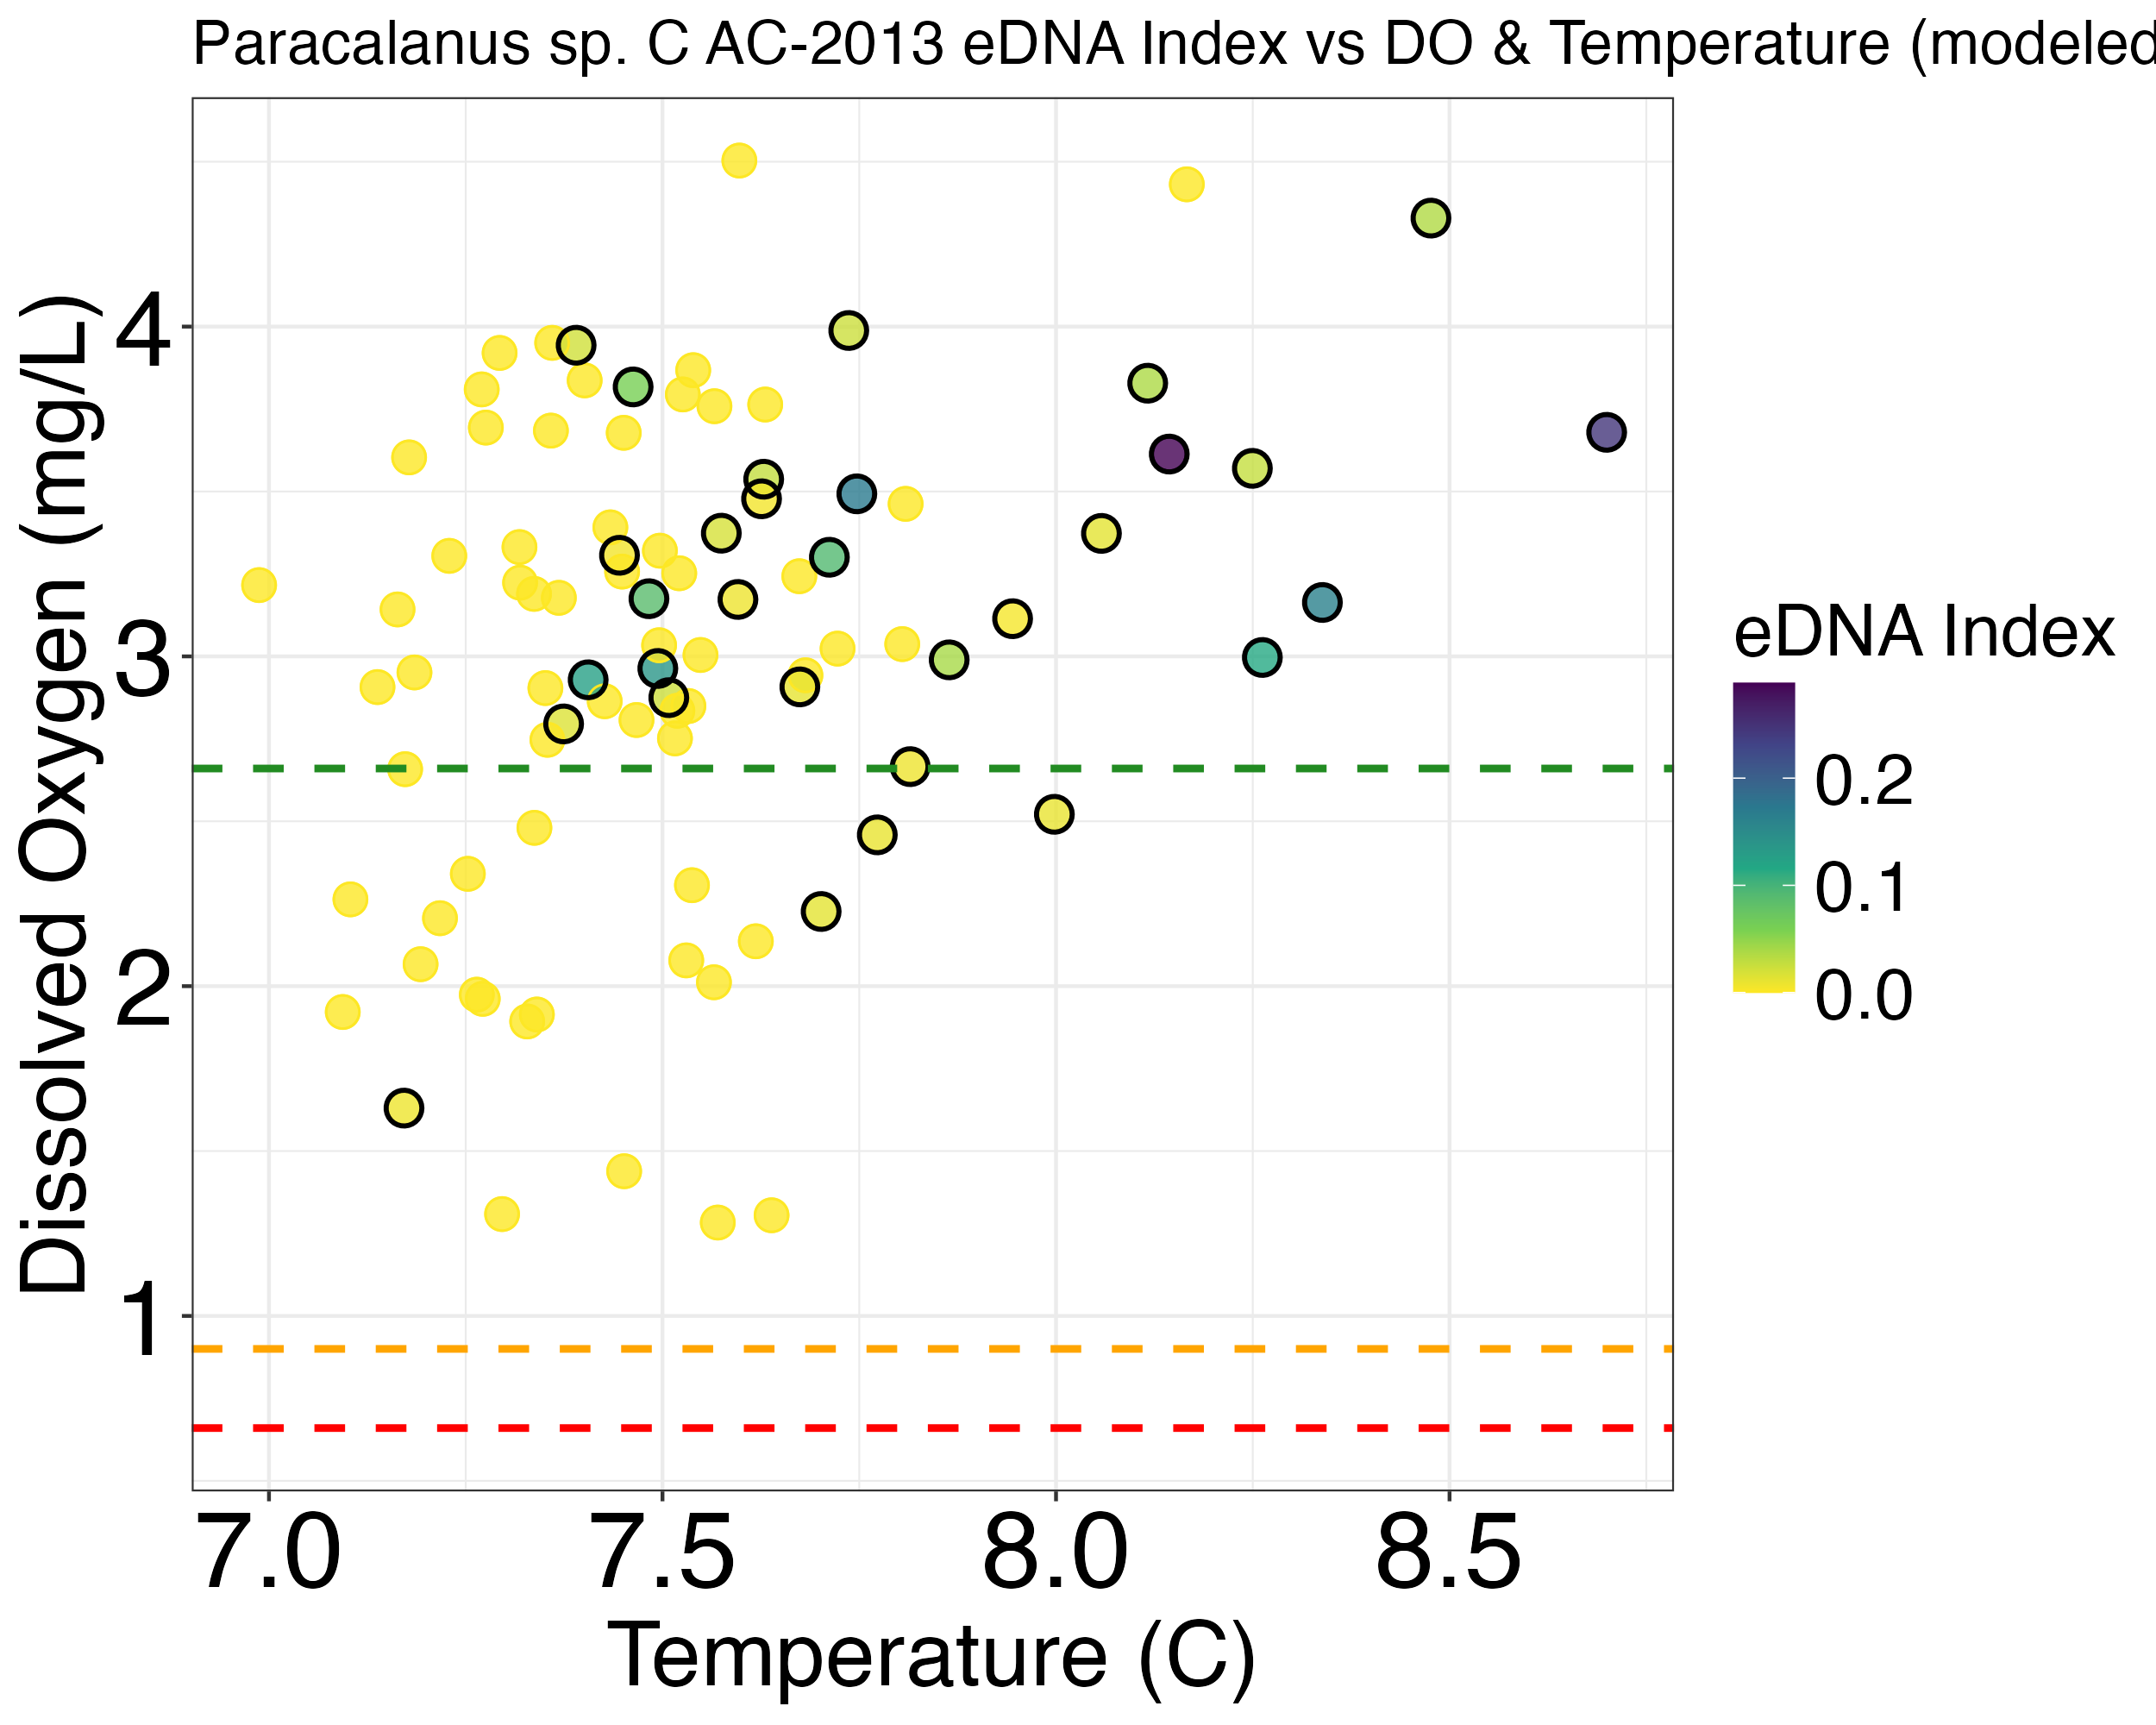
\includegraphics[scale=0.3]{Paracalanus_Scatter_AllYr_mod_noOut} 
			b. 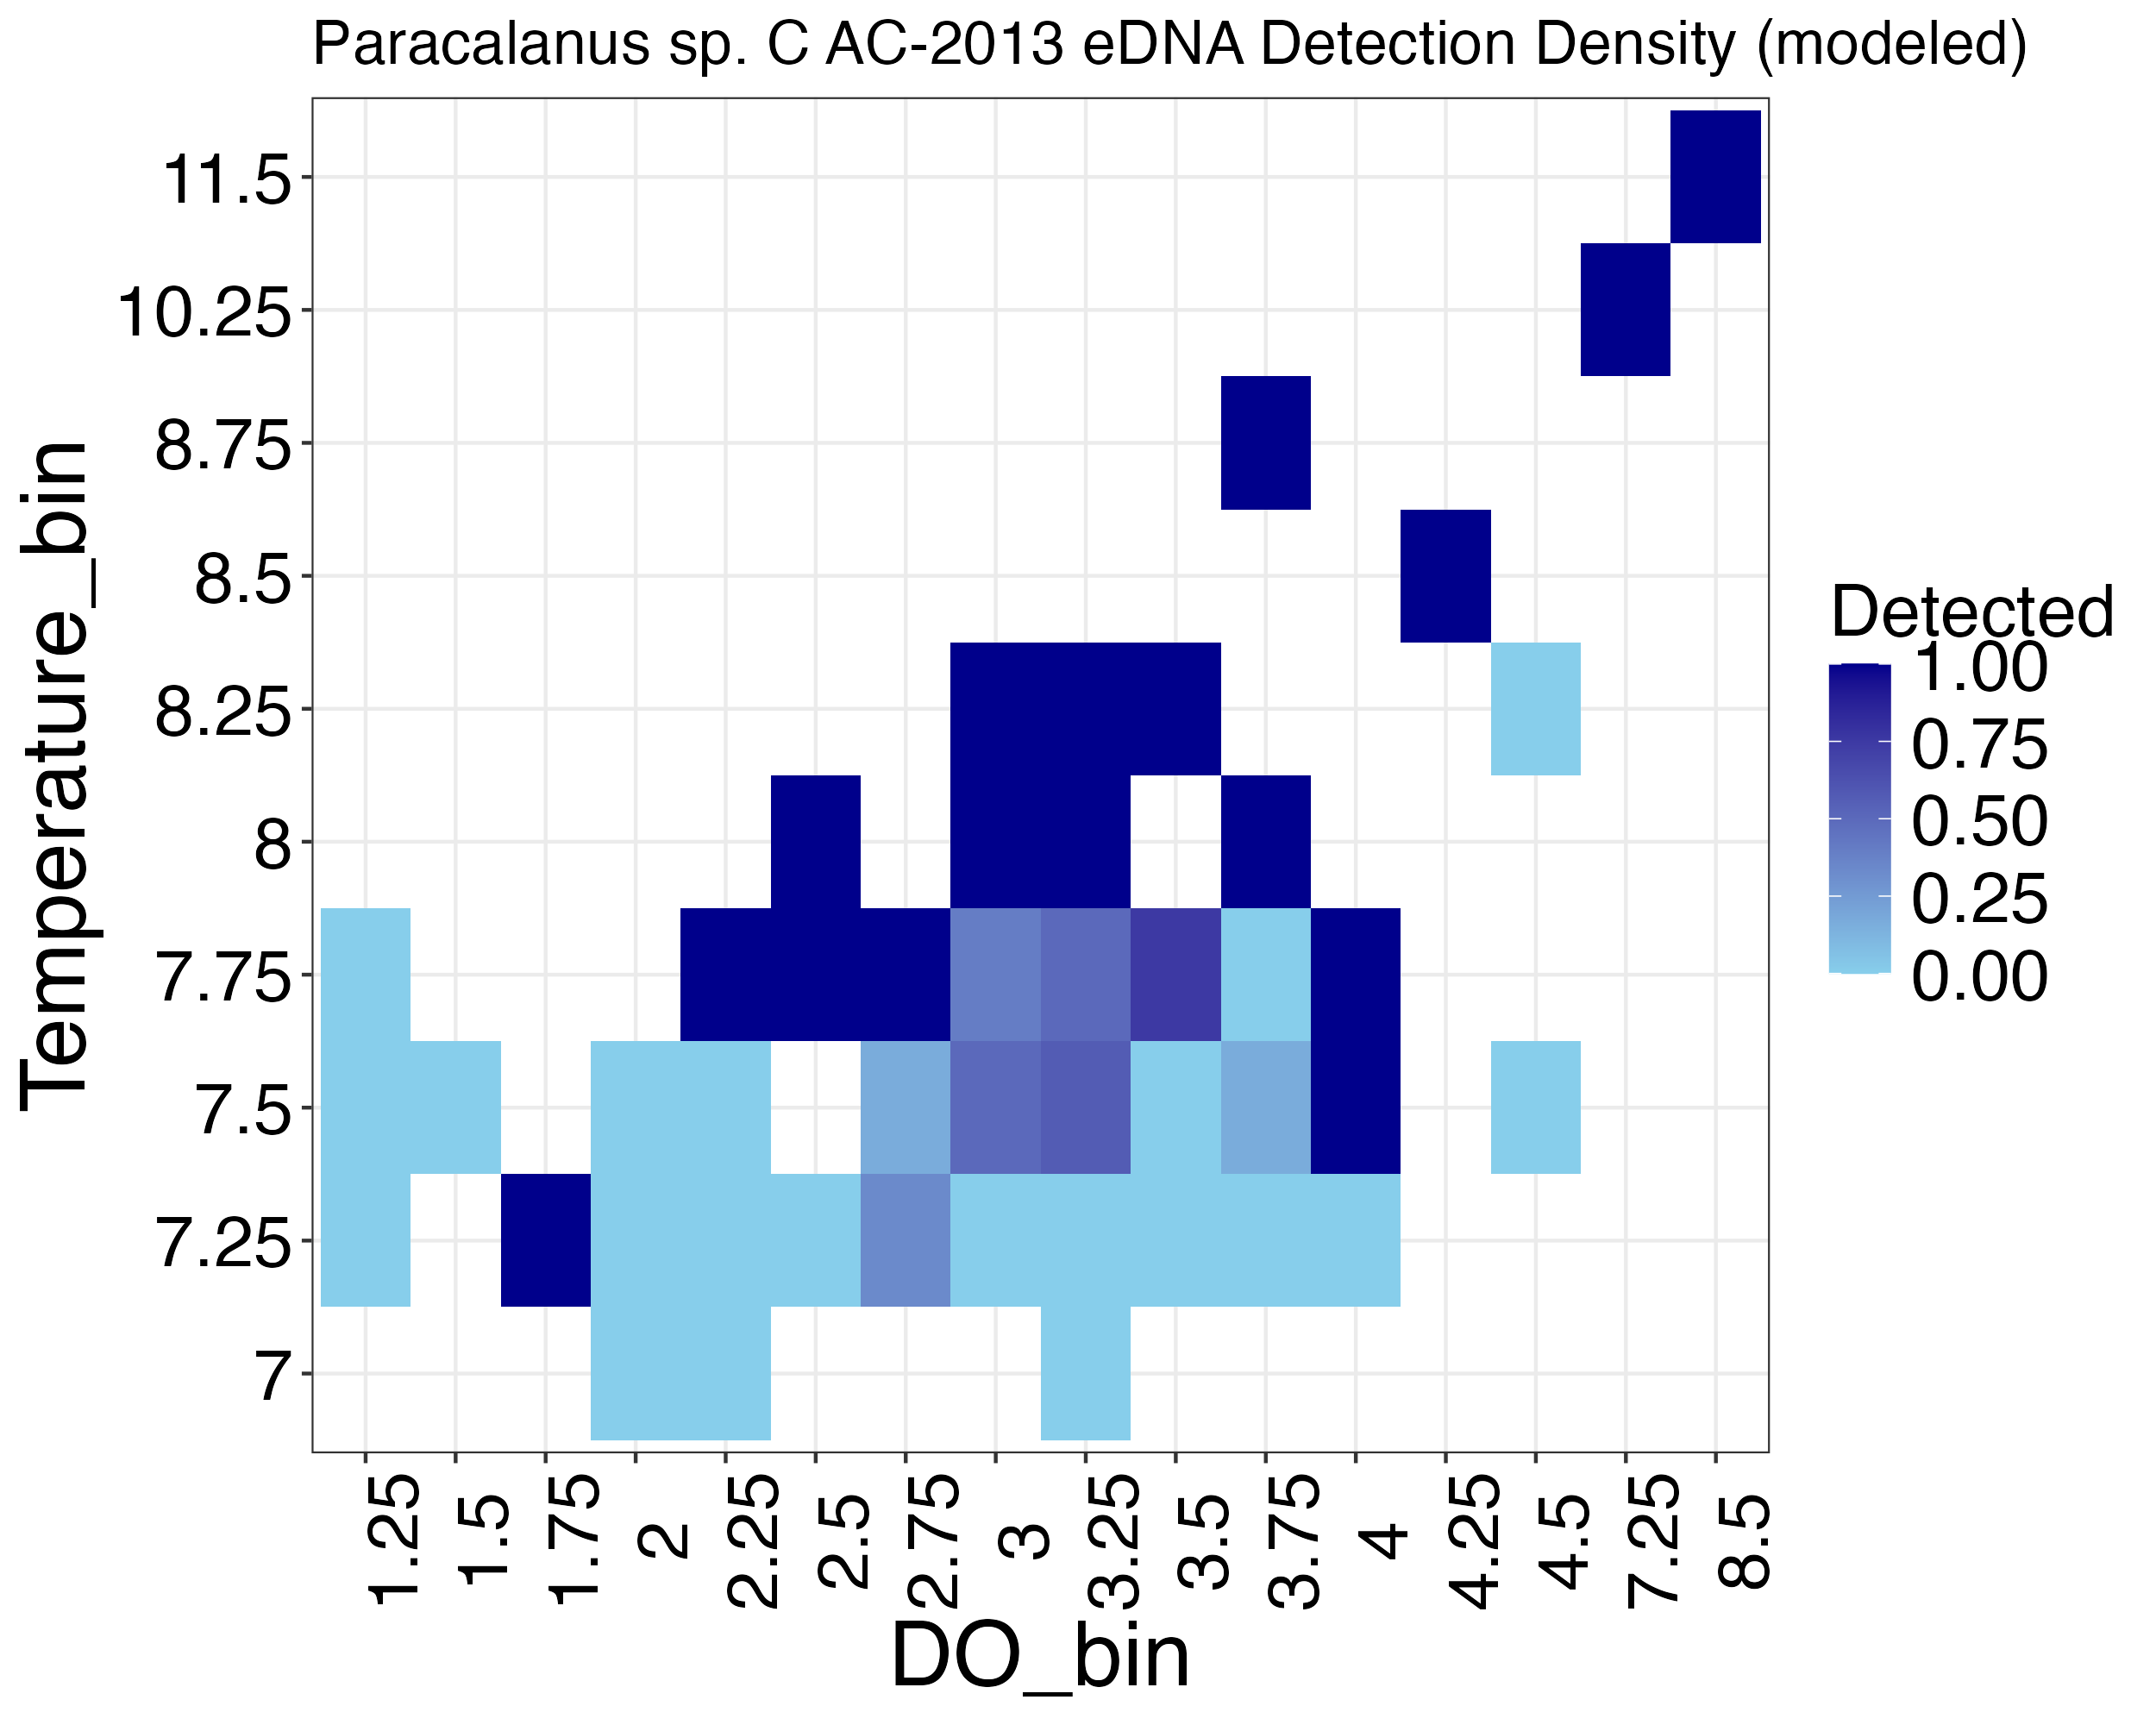
\includegraphics[scale=0.3]{Paracalanus_Density_AllYr_mod} 
			\caption[\textit{Paracalanus} sp. C AC-2013 scatterplot and density plot]{\footnotesize{\textit{Paracalanus} sp. C AC-2013 abundance and prevalence plots using LiveOcean model data from 2021-23.(a) Scatterplot of dissolved oxygen (mg/L) and temperature (Celsius) for each environmental DNA sampling time, with \textit{Paracalanus} sp. C AC-2013 scatterplot detections circled in black. Color represents eDNA index, a normalized measure of abundance that can compare abundance within a species. Yellow, uncircled dots represent sampling dates when \textit{Paracalanus} sp. C AC-2013 was not detected. (b) Density plot of \textit{Paracalanus} sp. C AC-2013 detections. Each pixel represents a range of dissolved oxygen and temperature values, and the shade of each pixel represents the proportion of eDNA samples in that environmental range in which \textit{Paracalanus} sp. C AC-2013 was detected. }} %the special ToC caption is in square brackets. The \footnotesize makes the figure caption smaller
			\label{ParacalanusScatter}
		\end{center}
	\end{figure} 
	
	
	\chapter{Discussion}
	
	Most of the copepods in this dataset with sufficiently large sample sizes were less abundant at lower dissolved oxygen levels, indicating that the levels of hypoxia in OCNMS during this study period were low enough to negatively impact copepod populations, regardless of whether the copepods were northern or southern. My results demonstrate that there was substantial inter-specific variability in whether copepod abundance changed with dissolved oxygen. Northern copepods were generally more abundant at higher dissolved oxygen levels. Only one southern copepod, \textit{Paracalanus} sp. C AC-2013, was detected more than 5 times in the dataset, and so it is difficult to draw overall conclusions about the hypoxia sensitivity of southern copepods. 
	
	The only copepod with more than 5 detections to have abundance negatively correlated with dissolved oxygen was \textit{O. similis}, which is generally considered neither northern nor southern and is abundant year-round off the coasts of Oregon and Washington. \textit{O. similis} was detected 11 times in the dataset, so future study is warranted before drawing conclusions, but it is possible that \textit{O. similis} has a higher tolerance to hypoxia than other copepods, and its abundance increases due to decreased competition during hypoxic events. The genus \textit{Oithona} has been used as an indicator of low oxygen conditions \autocite{Richard2001} and is known to have high hypoxia tolerance \autocite{Roman1993}, so this result is unsurprising. 
	
	The size patterns found in this study are generally consistent with the existing literature on copepod hypoxia tolerance. Previous studies have found that smaller copepods are more hypoxia tolerant, which is likely due to their larger surface area to volume ratio because copepods take up oxygen all over their bodies \autocite{Portner2010, Roman2019}. This study found that most smaller copepods were detected below 0.6 mg/L of oxygen, while several medium and large copepods were not. This supports the theory that smaller copepods are more hypoxia-tolerant and indicates that eDNA index can be a useful tool for investigating copepod environmental tolerance. However, this result should be interpreted with caution, as smaller copepods were detected many more times in this dataset than medium or large copepods. Copepod size depends on sex and age, which eDNA cannot discern, but we can still consider smaller and larger species in aggregate based on their known size ranges. 
	
	Observed patterns of detection and abundance at different temperatures aligned with the expected difference between northern and southern copepod ranges. Northern copepods were generally not detected above 8 ºC, and southern copepods were primarily detected above 7.5 ºC. Northern copepods are known to inhabit cold water, and southern copepods are known to inhabit warm water, so this aligns with existing knowledge of these two groups of copepods. 
	
	Global climate change models predict that upwelling in the northern region of the California Current system, where this study was located, will increase in strength and event duration in the future \autocite{Bograd2023}. While there is significant uncertainty in these models, upwelling has been increasing in severity in OCNMS, and it is important to consider the potential impacts if this trend continues. Increased upwelling would lead to colder temperatures and lower dissolved oxygen in OCNMS \autocite{Bograd2023}. Based on the results of this study, decreasing dissolved oxygen levels in OCNMS could lead to a decrease in overall copepod abundance, and a copepod community dominated by smaller species, southern copepods, and \textit{Oithona similis}. Lower temperatures due to increased upwelling could buffer this effect, as southern copepods would likely become less abundant and copepod hypoxia tolerance declines in warmer conditions \autocite{Vaquer-Sunyer2011}. These trends would result in less copepod biomass available for juvenile salmon and other fish in OCNMS, which could lead to a decrease in abundance of culturally and economically important fish species. Future studies should investigate the effects of hypoxia on other fish prey species, to determine if juvenile salmon and other fish could be expected to switch to more hypoxia-tolerant prey in a future with increased upwelling.
	
	It is worth noting that the entire period of this study, 2021-2023, took place during negative Pacific Decadal Oscillation (PDO) and negative Oceanic Niño Index (ONI) years, meaning that this study took place in relatively cold conditions. The Pacific Decadal Oscillation (PDO) is a climatological index used to describe broad shifts in the Pacific Ocean and the atmosphere above it. Cooler periods are described as negative PDO periods, and warm periods are described as positive PDO years. ONI is an index used to describe the El Niño Southern Oscillation (ENSO), a climate pattern in the tropical Pacific that changes every two to seven years. ONI is the three-month running mean of sea surface temperature anomalies in a specific region of the Pacific Ocean \autocite{ClimatePredictionCenterInternetTeam}. During El Niño events, characterized by a positive ONI, the central and eastern tropical Pacific Ocean warm and the west coast of North America warms \autocite{LHeureux2014}. During positive PDO or positive ONI (El Niño events) periods, copepod species richness on the west coast of North America is high \autocite{NOAAFisheries2024}. Because of this, we expect lower species richness during the period of this study than during positive ENSO years, so some species may be missing from this study. In the future, the automated eDNA sampler in OCNMS will hopefully collect data during a positive ENSO year and acquire more data, improving the generalizability of any studies conducted using this data. 
	
	While eDNA index is not a perfect metric of abundance, it is still useful for broad studies such as this one when it is the only data available. eDNA can detect species with relatively high spatial resolution, from as little as 60 meters in a kelp forest \autocite{Port2016} to 800 meters in deep-water habitats in Maizuru Bay, Japan \autocite{Yamamoto2017}, because eDNA levels drop below the detection limit soon after being released via diffusion and decay. However, our understanding of how far eDNA can migrate in the environment is still relatively limited, and eDNA dispersal and decay can be affected by a number of environmental factors \autocite{Cristescu2018}. 
	
	Copepods in the genera \textit{Paracalanus} and \textit{Acartia} in Puget Sound, an estuary close to this study's site, are known to behaviorally avoid hypoxia by remaining above hypoxic bottom water \autocite{Keister2013}. Therefore, the lower abundance in these genera found in this study could be the result of behavioral avoidance, and copepod populations may be moving to different depths. This study was limited to one point in space, but future studies using multiple automated eDNA samplers at different depths could determine whether declining copepod abundance in hypoxic conditions is due to population declines or population movements. 
	
	Copepod populations do not exist in isolation, and future studies should also consider the taxonomic effects of hypoxia. For example, if fish that eat copepods are more sensitive to hypoxia than the copepods themselves, decreased predation due to fish kills may lead to increased copepod populations at certain dissolved oxygen levels. If copepods are more sensitive to hypoxia than the fish that eat them, decreased prey availability may impact fish at levels of hypoxia that would otherwise be tolerable. Crustaceans and fish are both known to be highly sensitive to hypoxia compared to other taxonomic groups, so future studies into copepod hypoxia tolerance and copepod predator hypoxia tolerance will be important and should take individual species tolerances into account.
   
   	\appendix
   \chapter{Software and Data Availability}\label{chap:appR}
   
   \section{Data Availability Statement}
   
   All code used in this thesis can be found at https://github.com/DolphinCoder/Reed-Thesis-Copepod-Populations.
   
   The results of the overall automated eDNA sampler study in OCNMS are actively being organized into a peer-reviewed manuscript, and all data will be made available upon publication. Reach out to Zachary Gold (zachary.gold@noaa.gov) for more information or to request raw data.
     
     \section{R Packages Used}
	\begin{hangparas}{0.25in}{1}
	   \fullcite{Aphalo2024} \\
	   
	   \fullcite{Wickham2023a} \\
	   
	   \fullcite{Muller2020} \\
	   
	   \fullcite{Wickham2025} \\
	   
	   \fullcite{Burkner2024}  \\ 
	   
	   \fullcite{Wickham2023} \\
	   
	   \fullcite{Kay2024} \\
	   
	   \fullcite{Robinson2025} \\
	   
	   \fullcite{Bolker2024} \\
	   
	   \fullcite{Kay2025} \\
	   
	   \fullcite{Pierce2025}  \\ 
	   
   \end{hangparas}

%If you feel it necessary to include an appendix, it goes here.
    \chapter{Zero-Inflated Beta Regression Plots}\label{chap:appZOIB}

	\begin{figure}[h]
		\begin{center}
			Northern: \\
			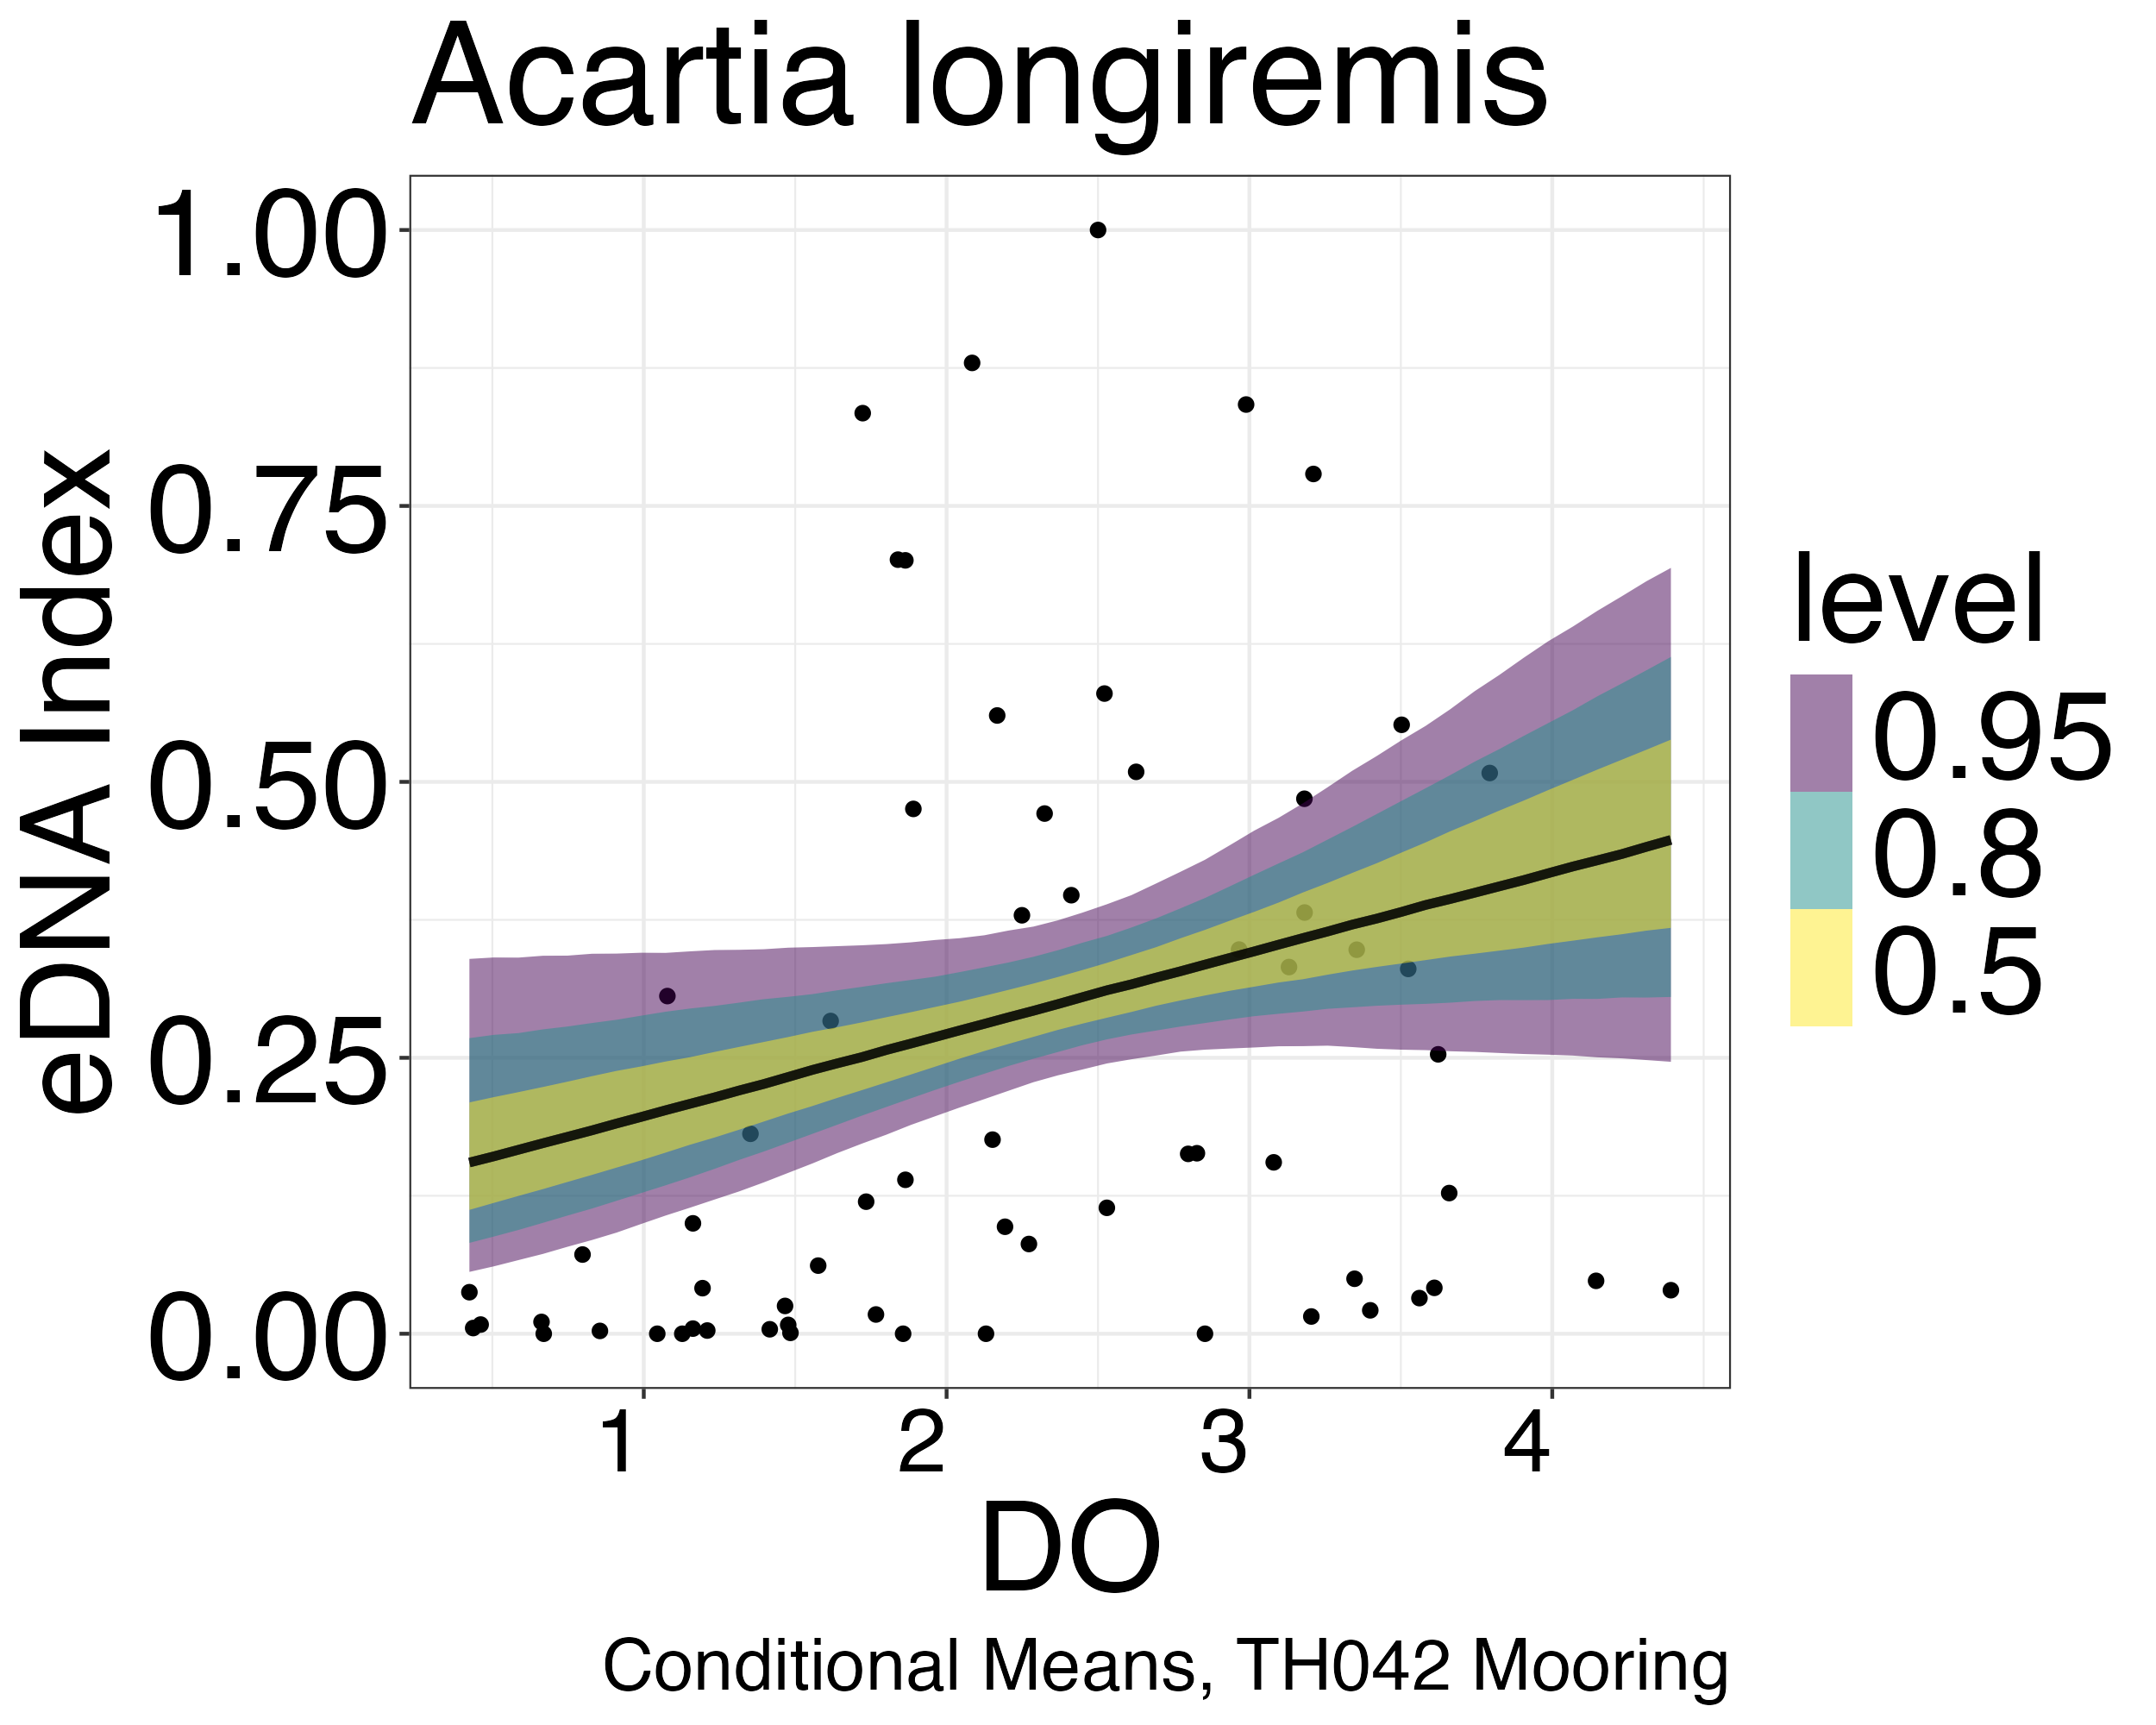
\includegraphics[scale=0.25]{Alongiremis_ZOIB_Means_noOut}
			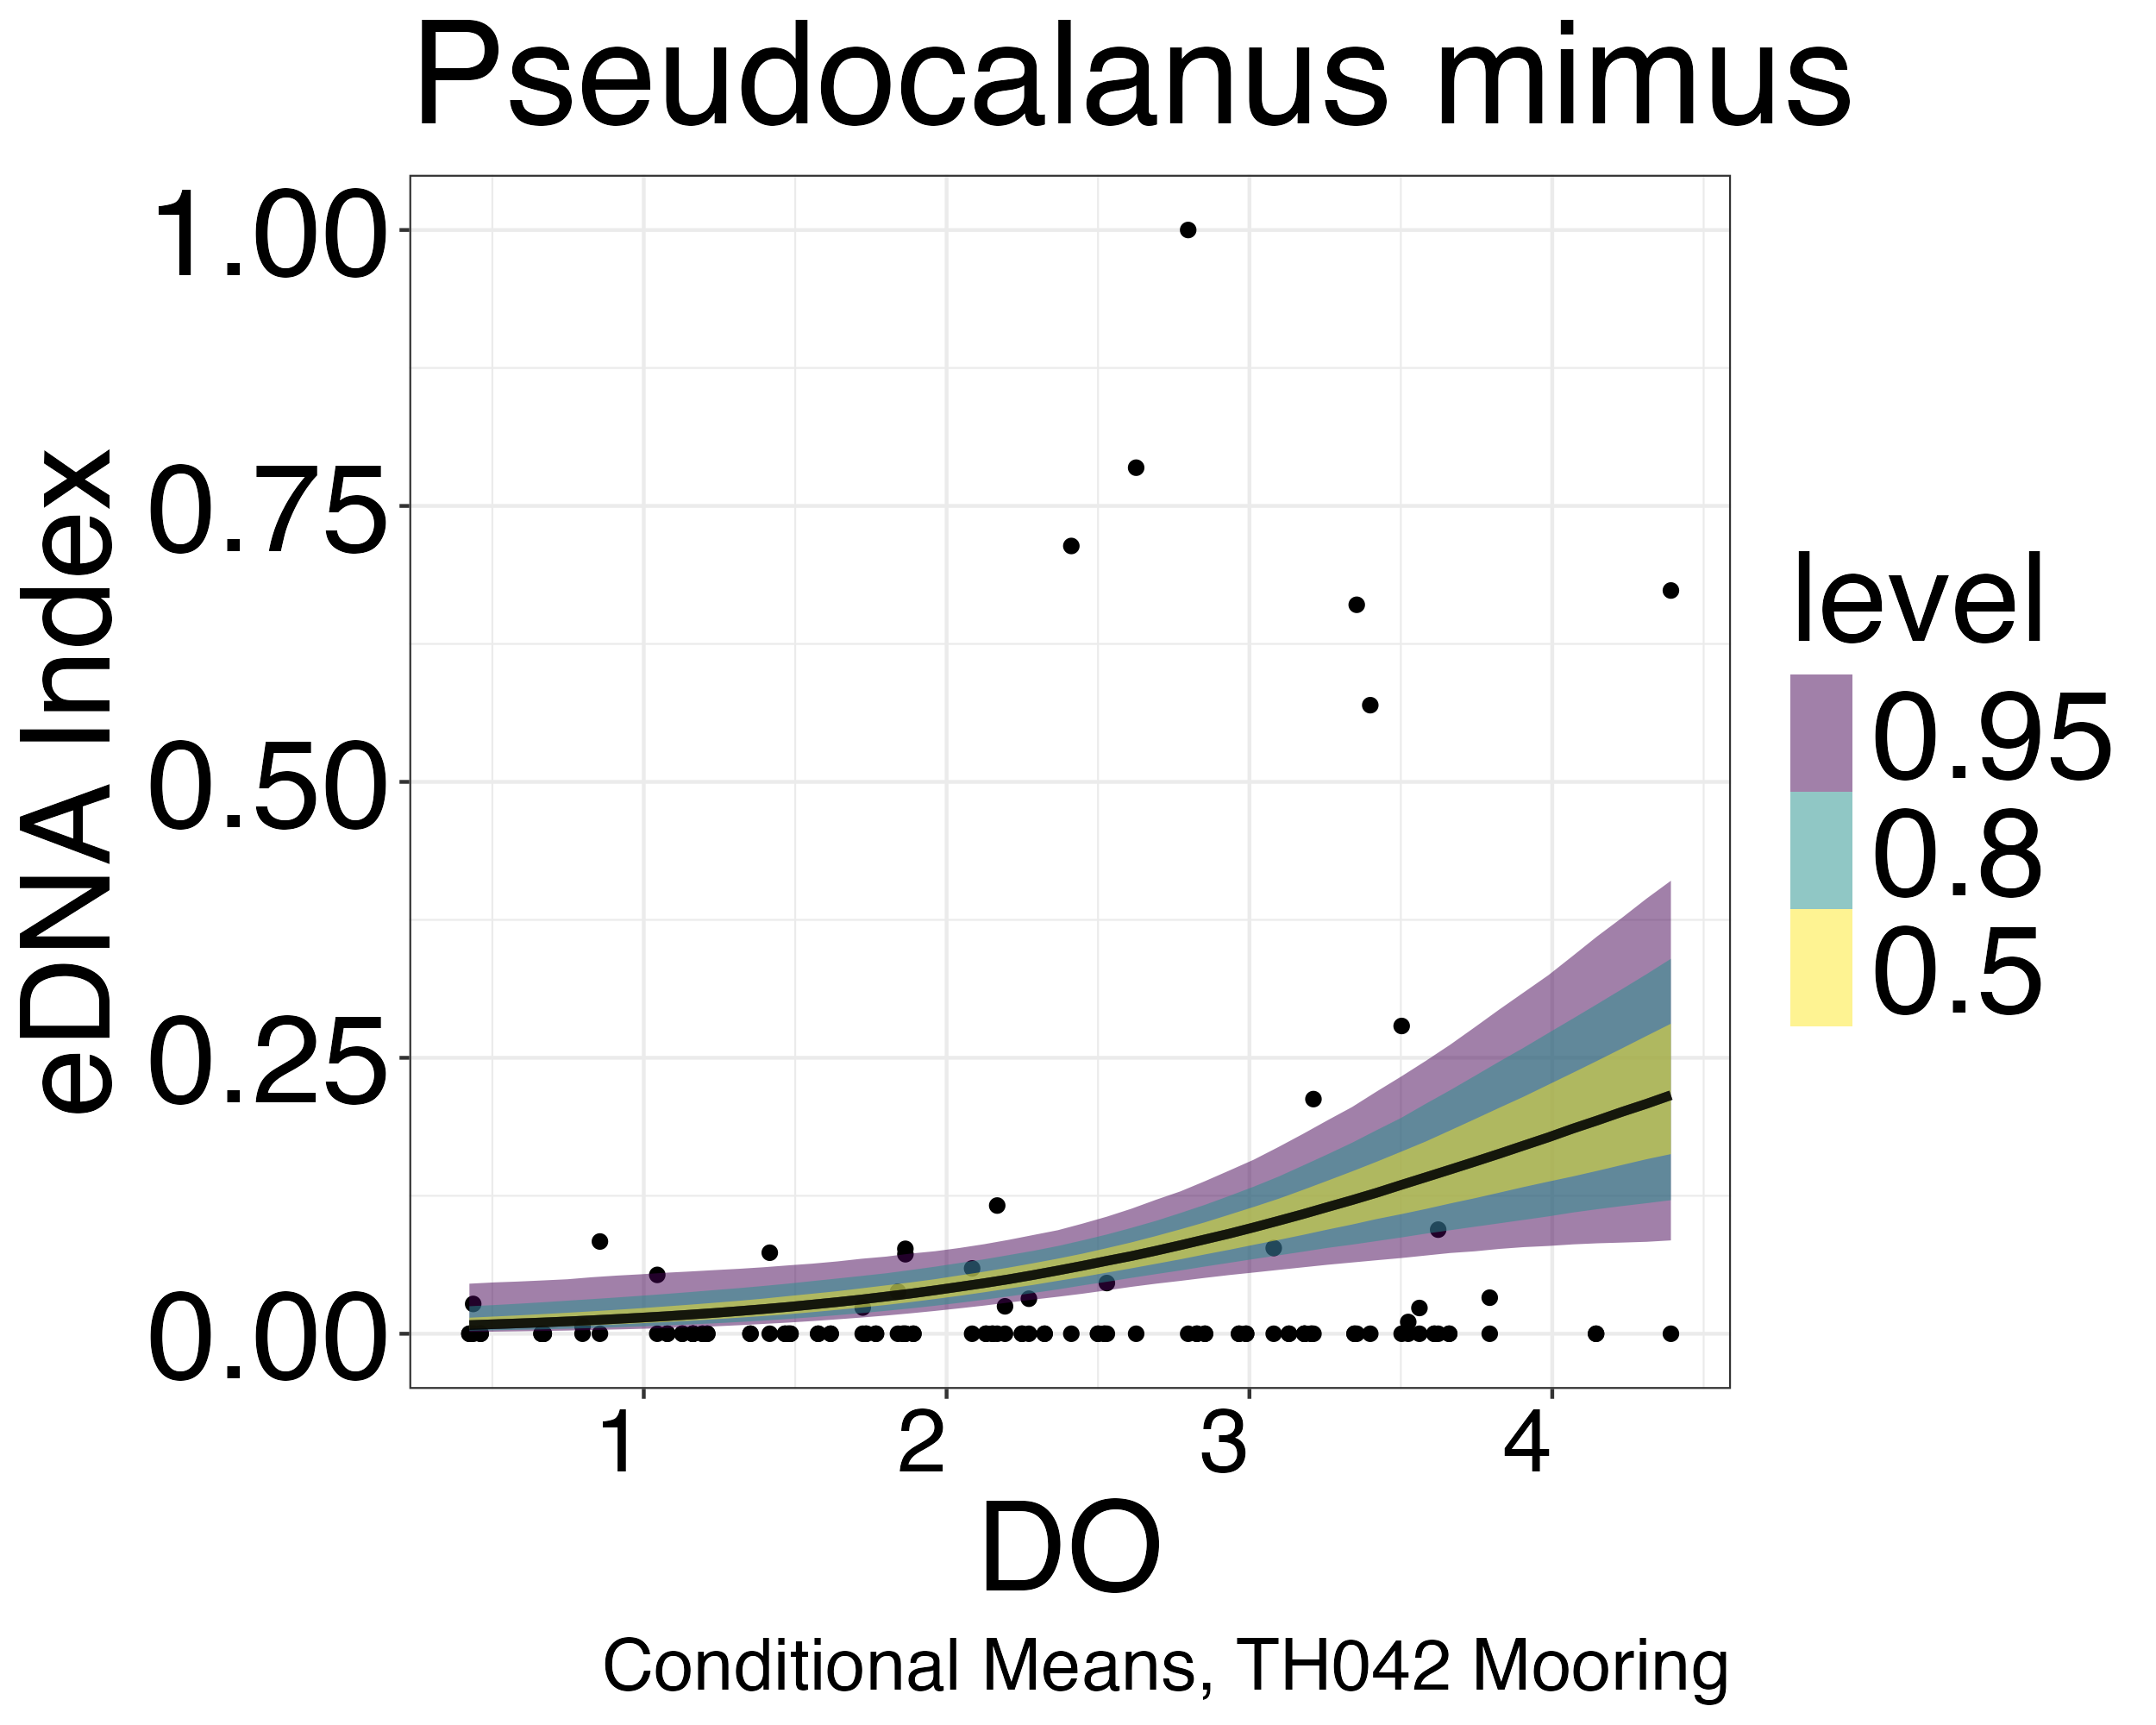
\includegraphics[scale=0.25]{Pmimus_ZOIB_Means_noOut}
			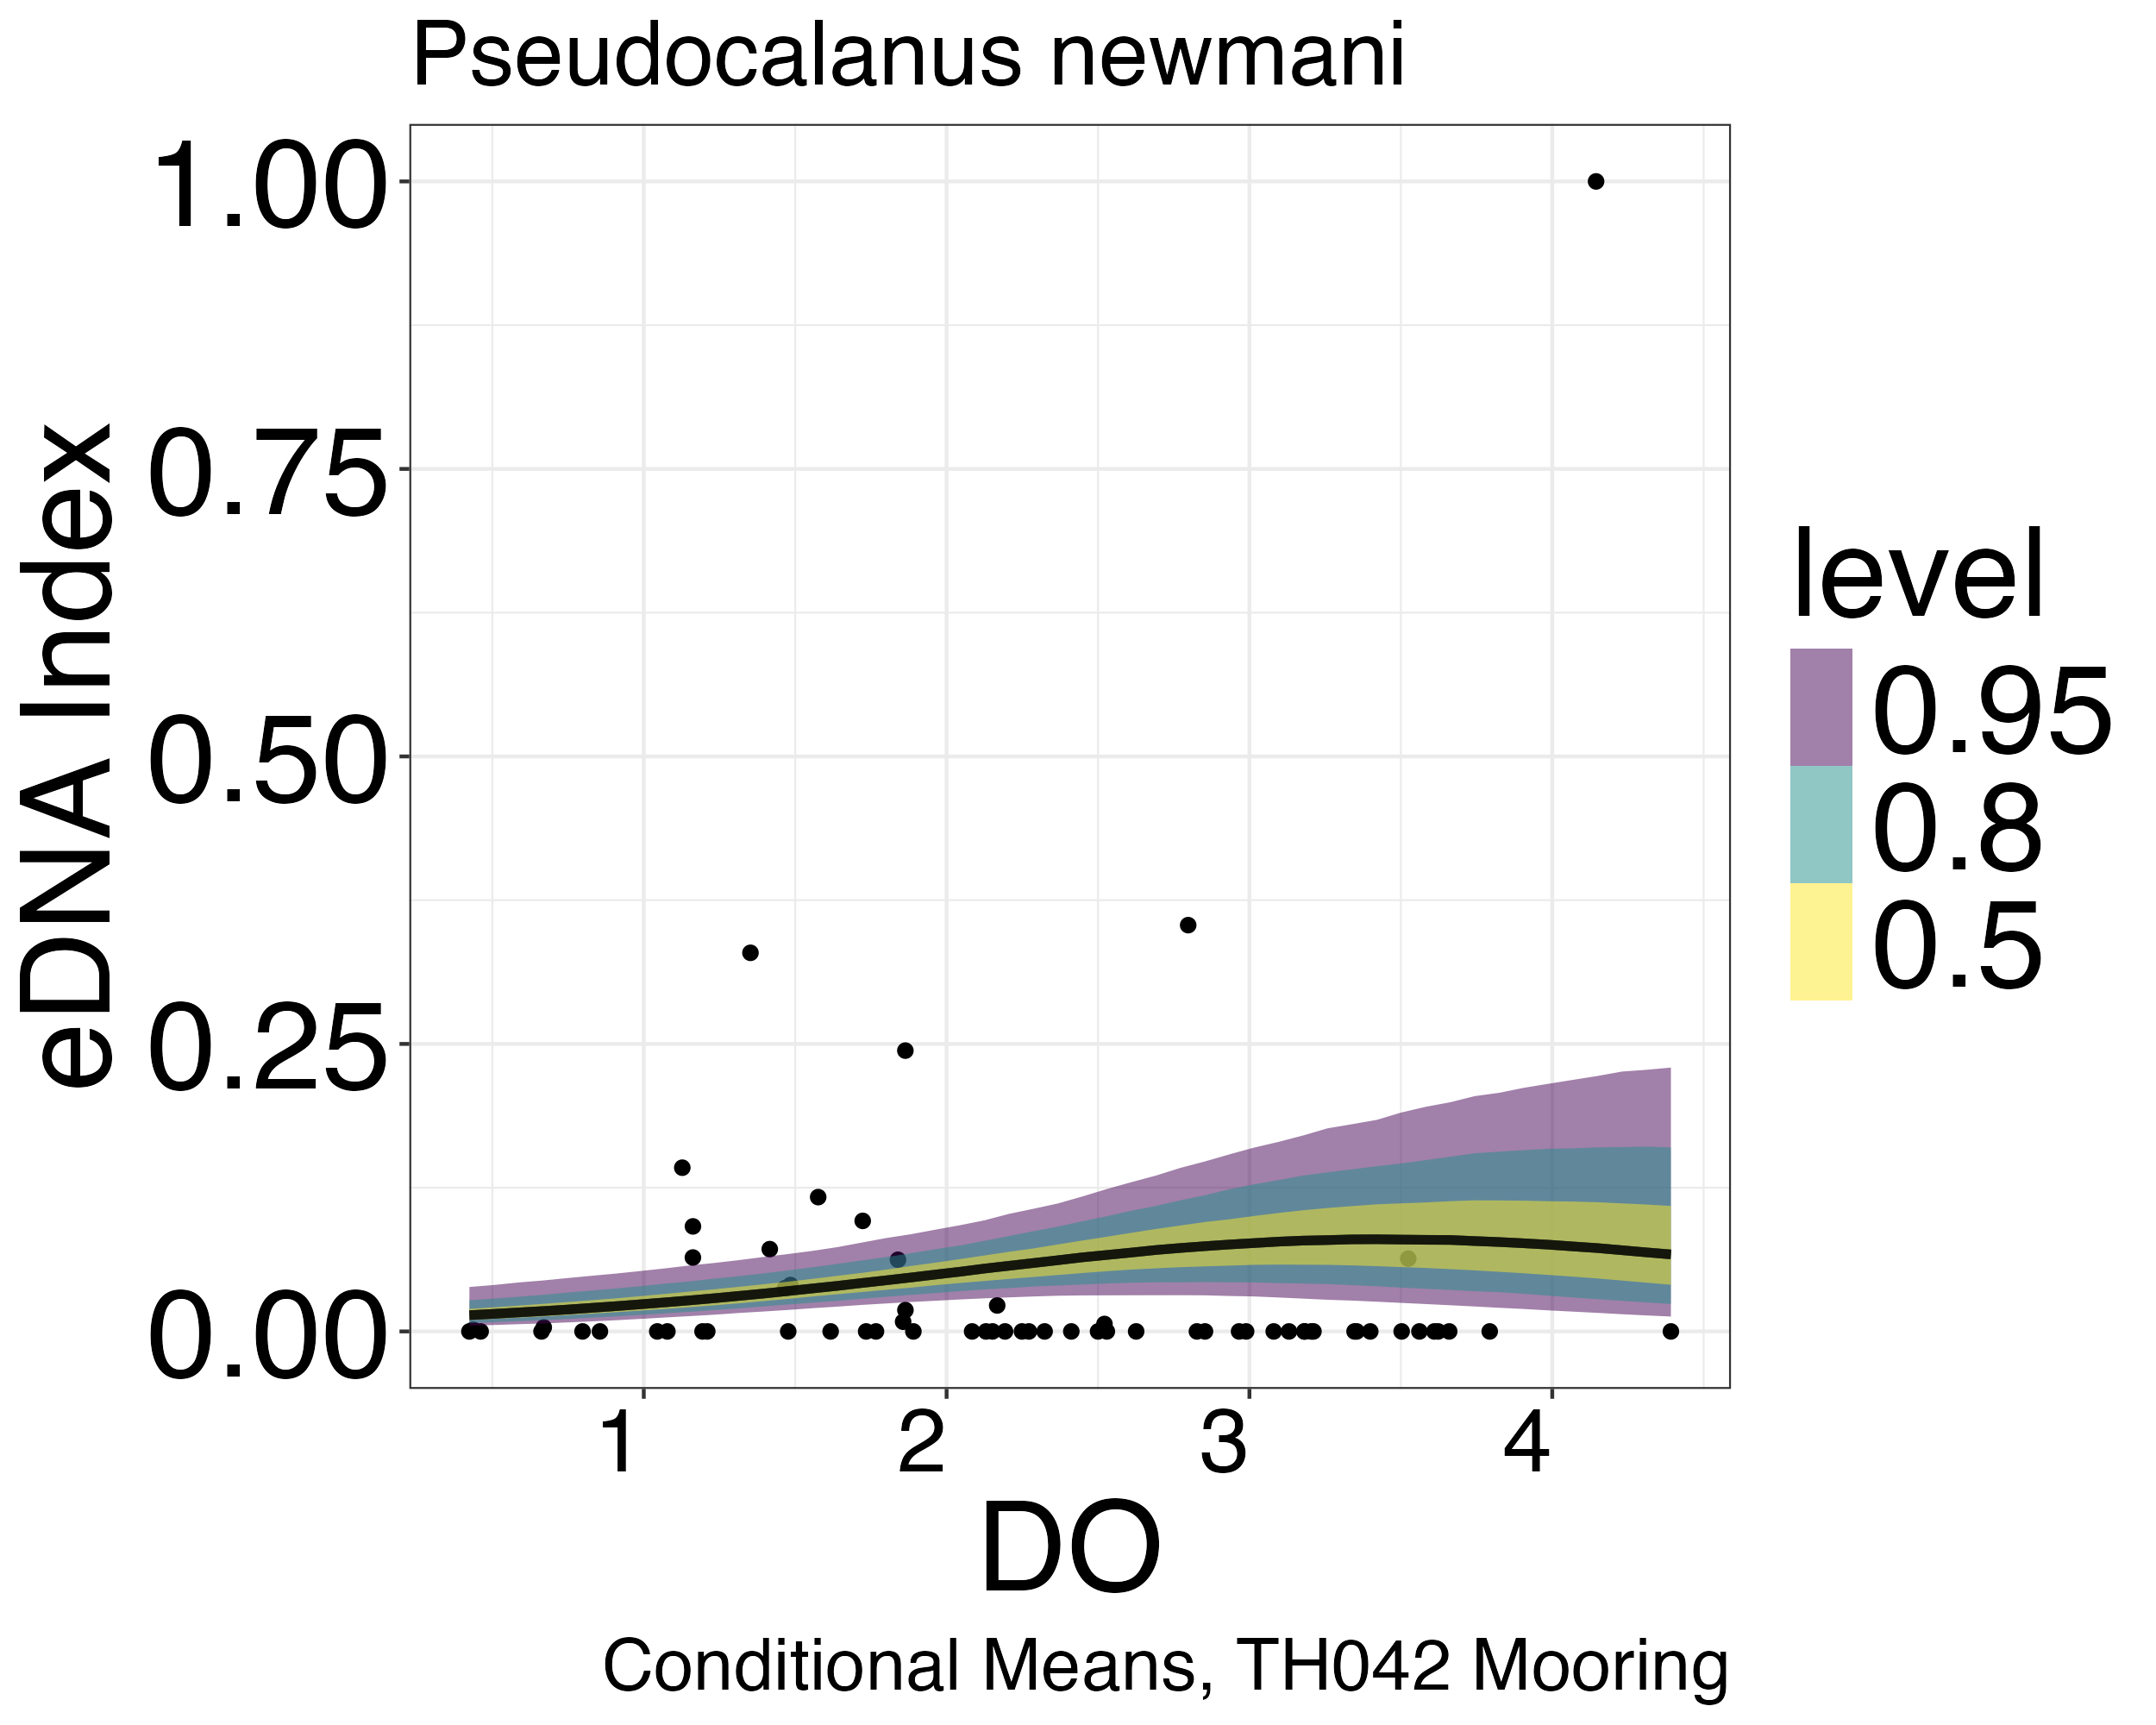
\includegraphics[scale=0.25]{Pnewmani_ZOIB_Means_noOut}
			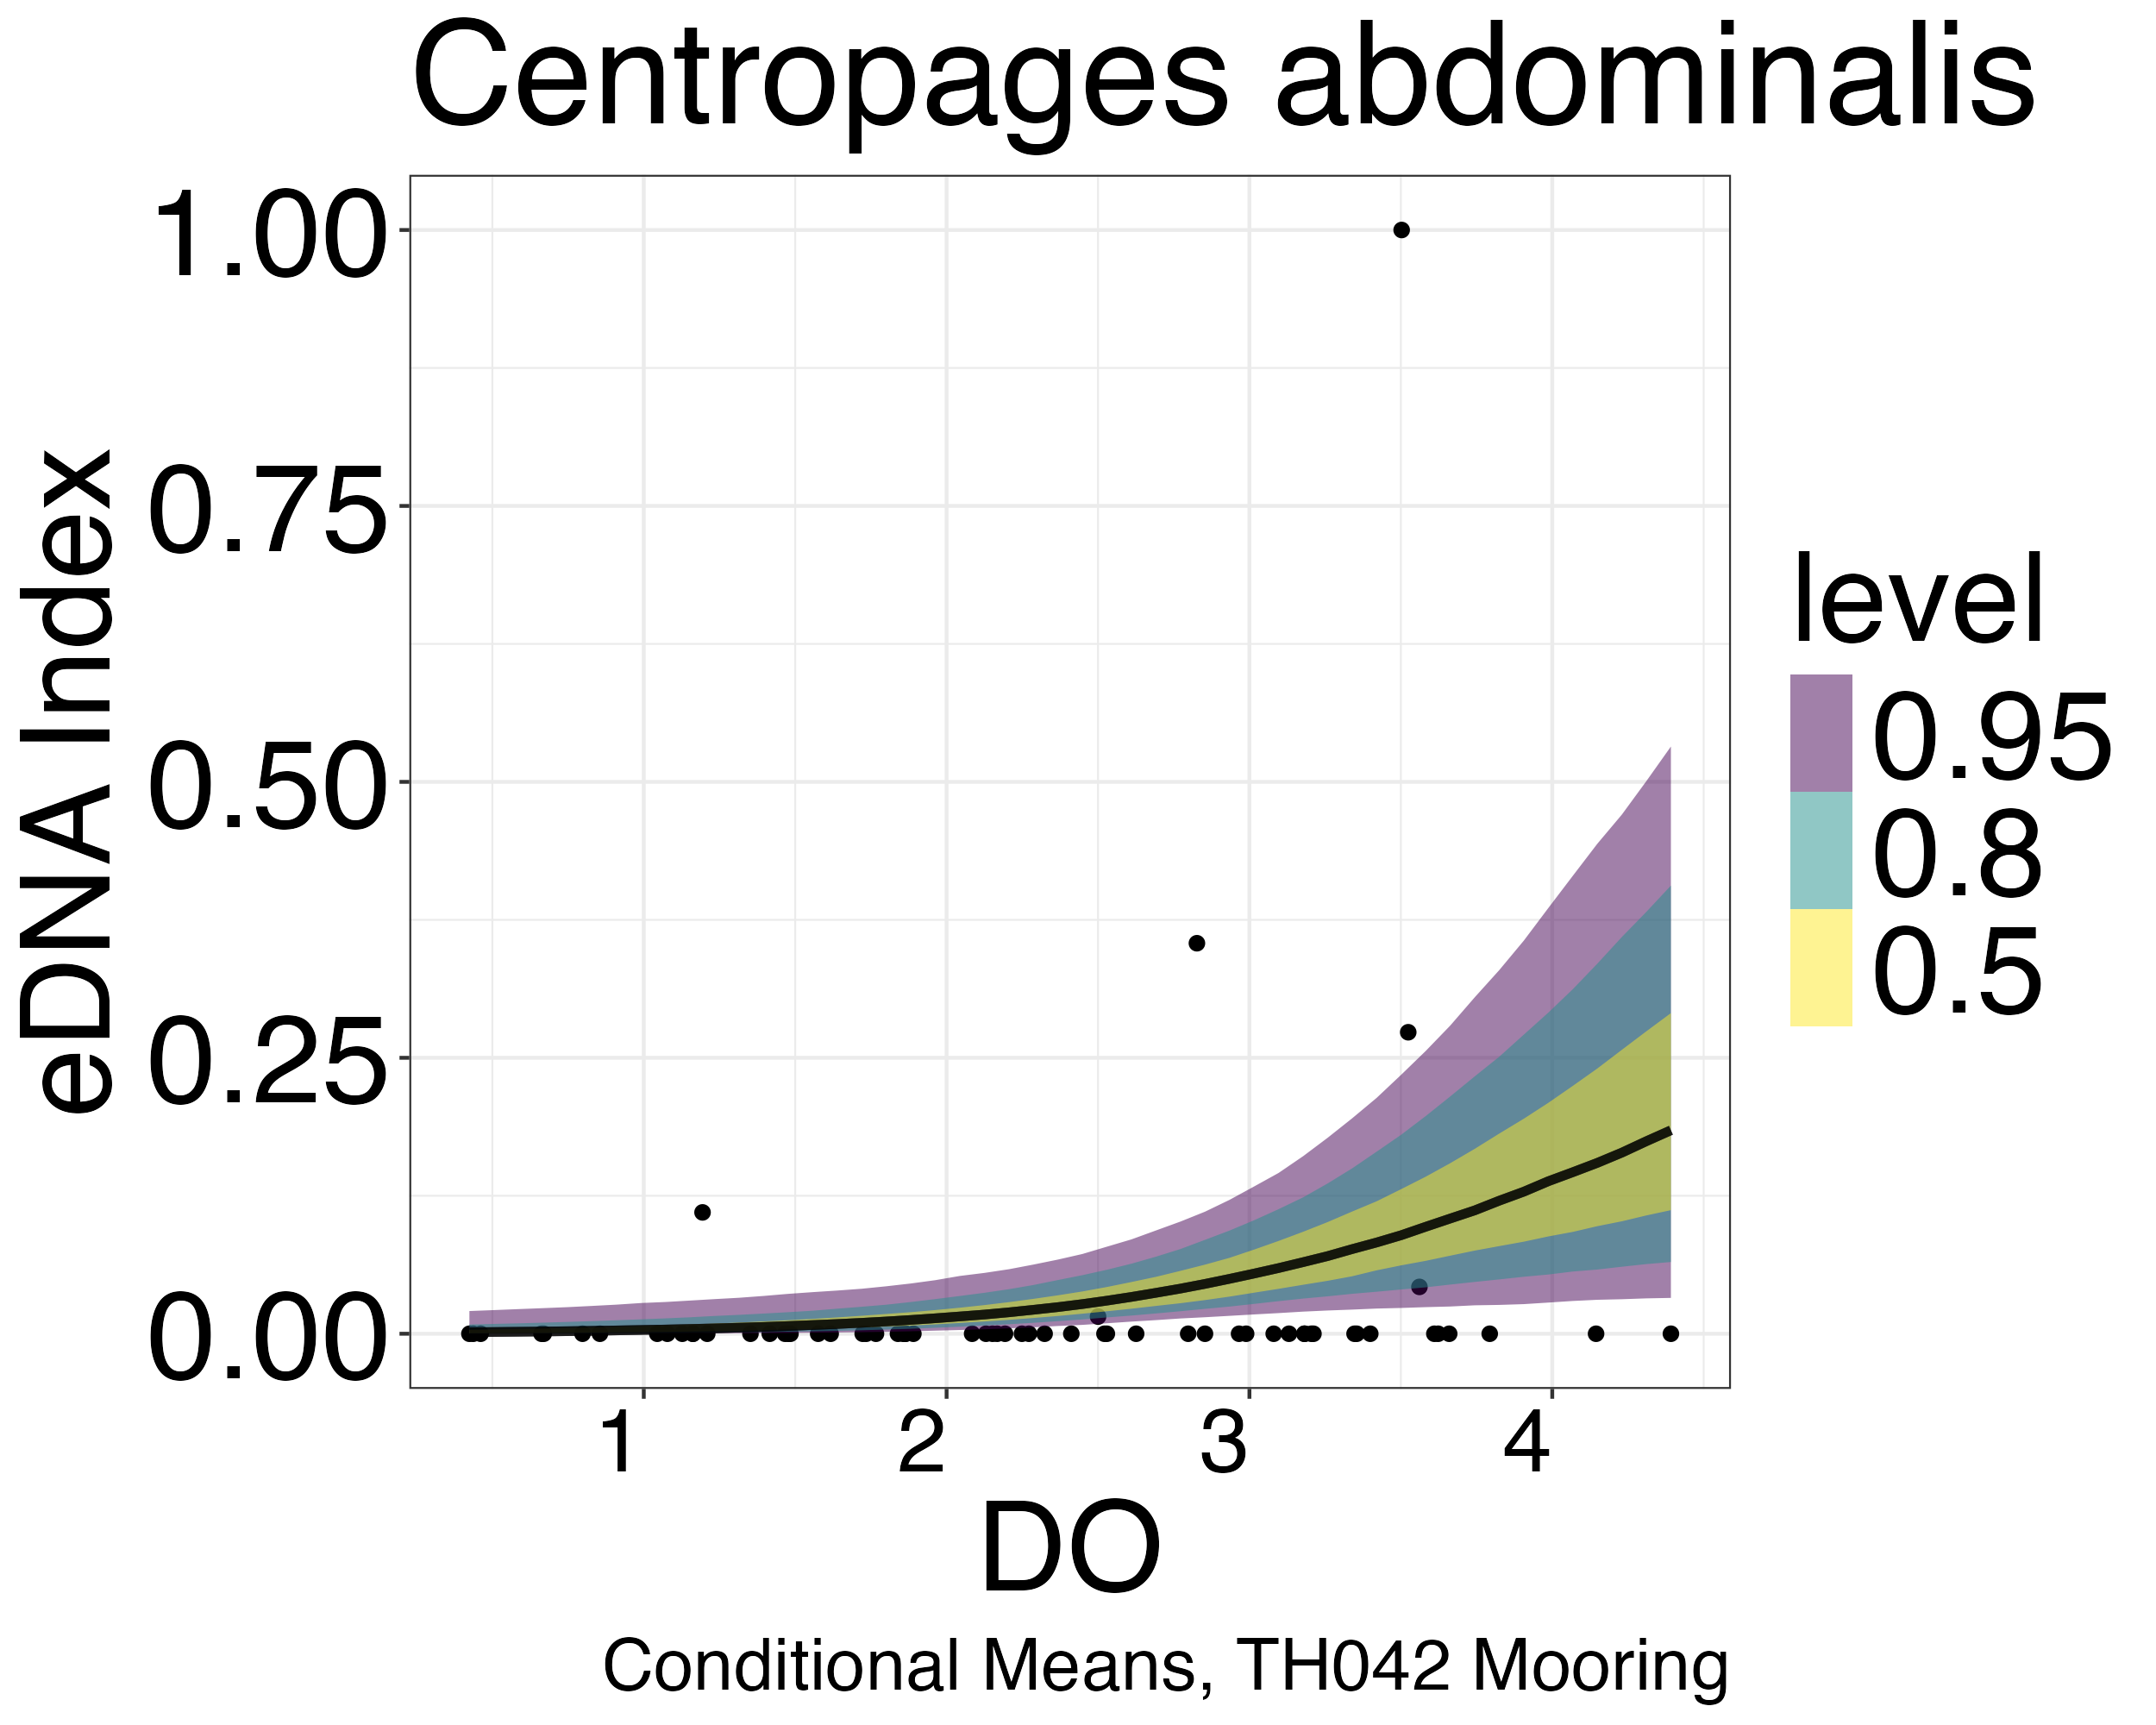
\includegraphics[scale=0.25]{Cabdominalis_ZOIB_Means_noOut}
			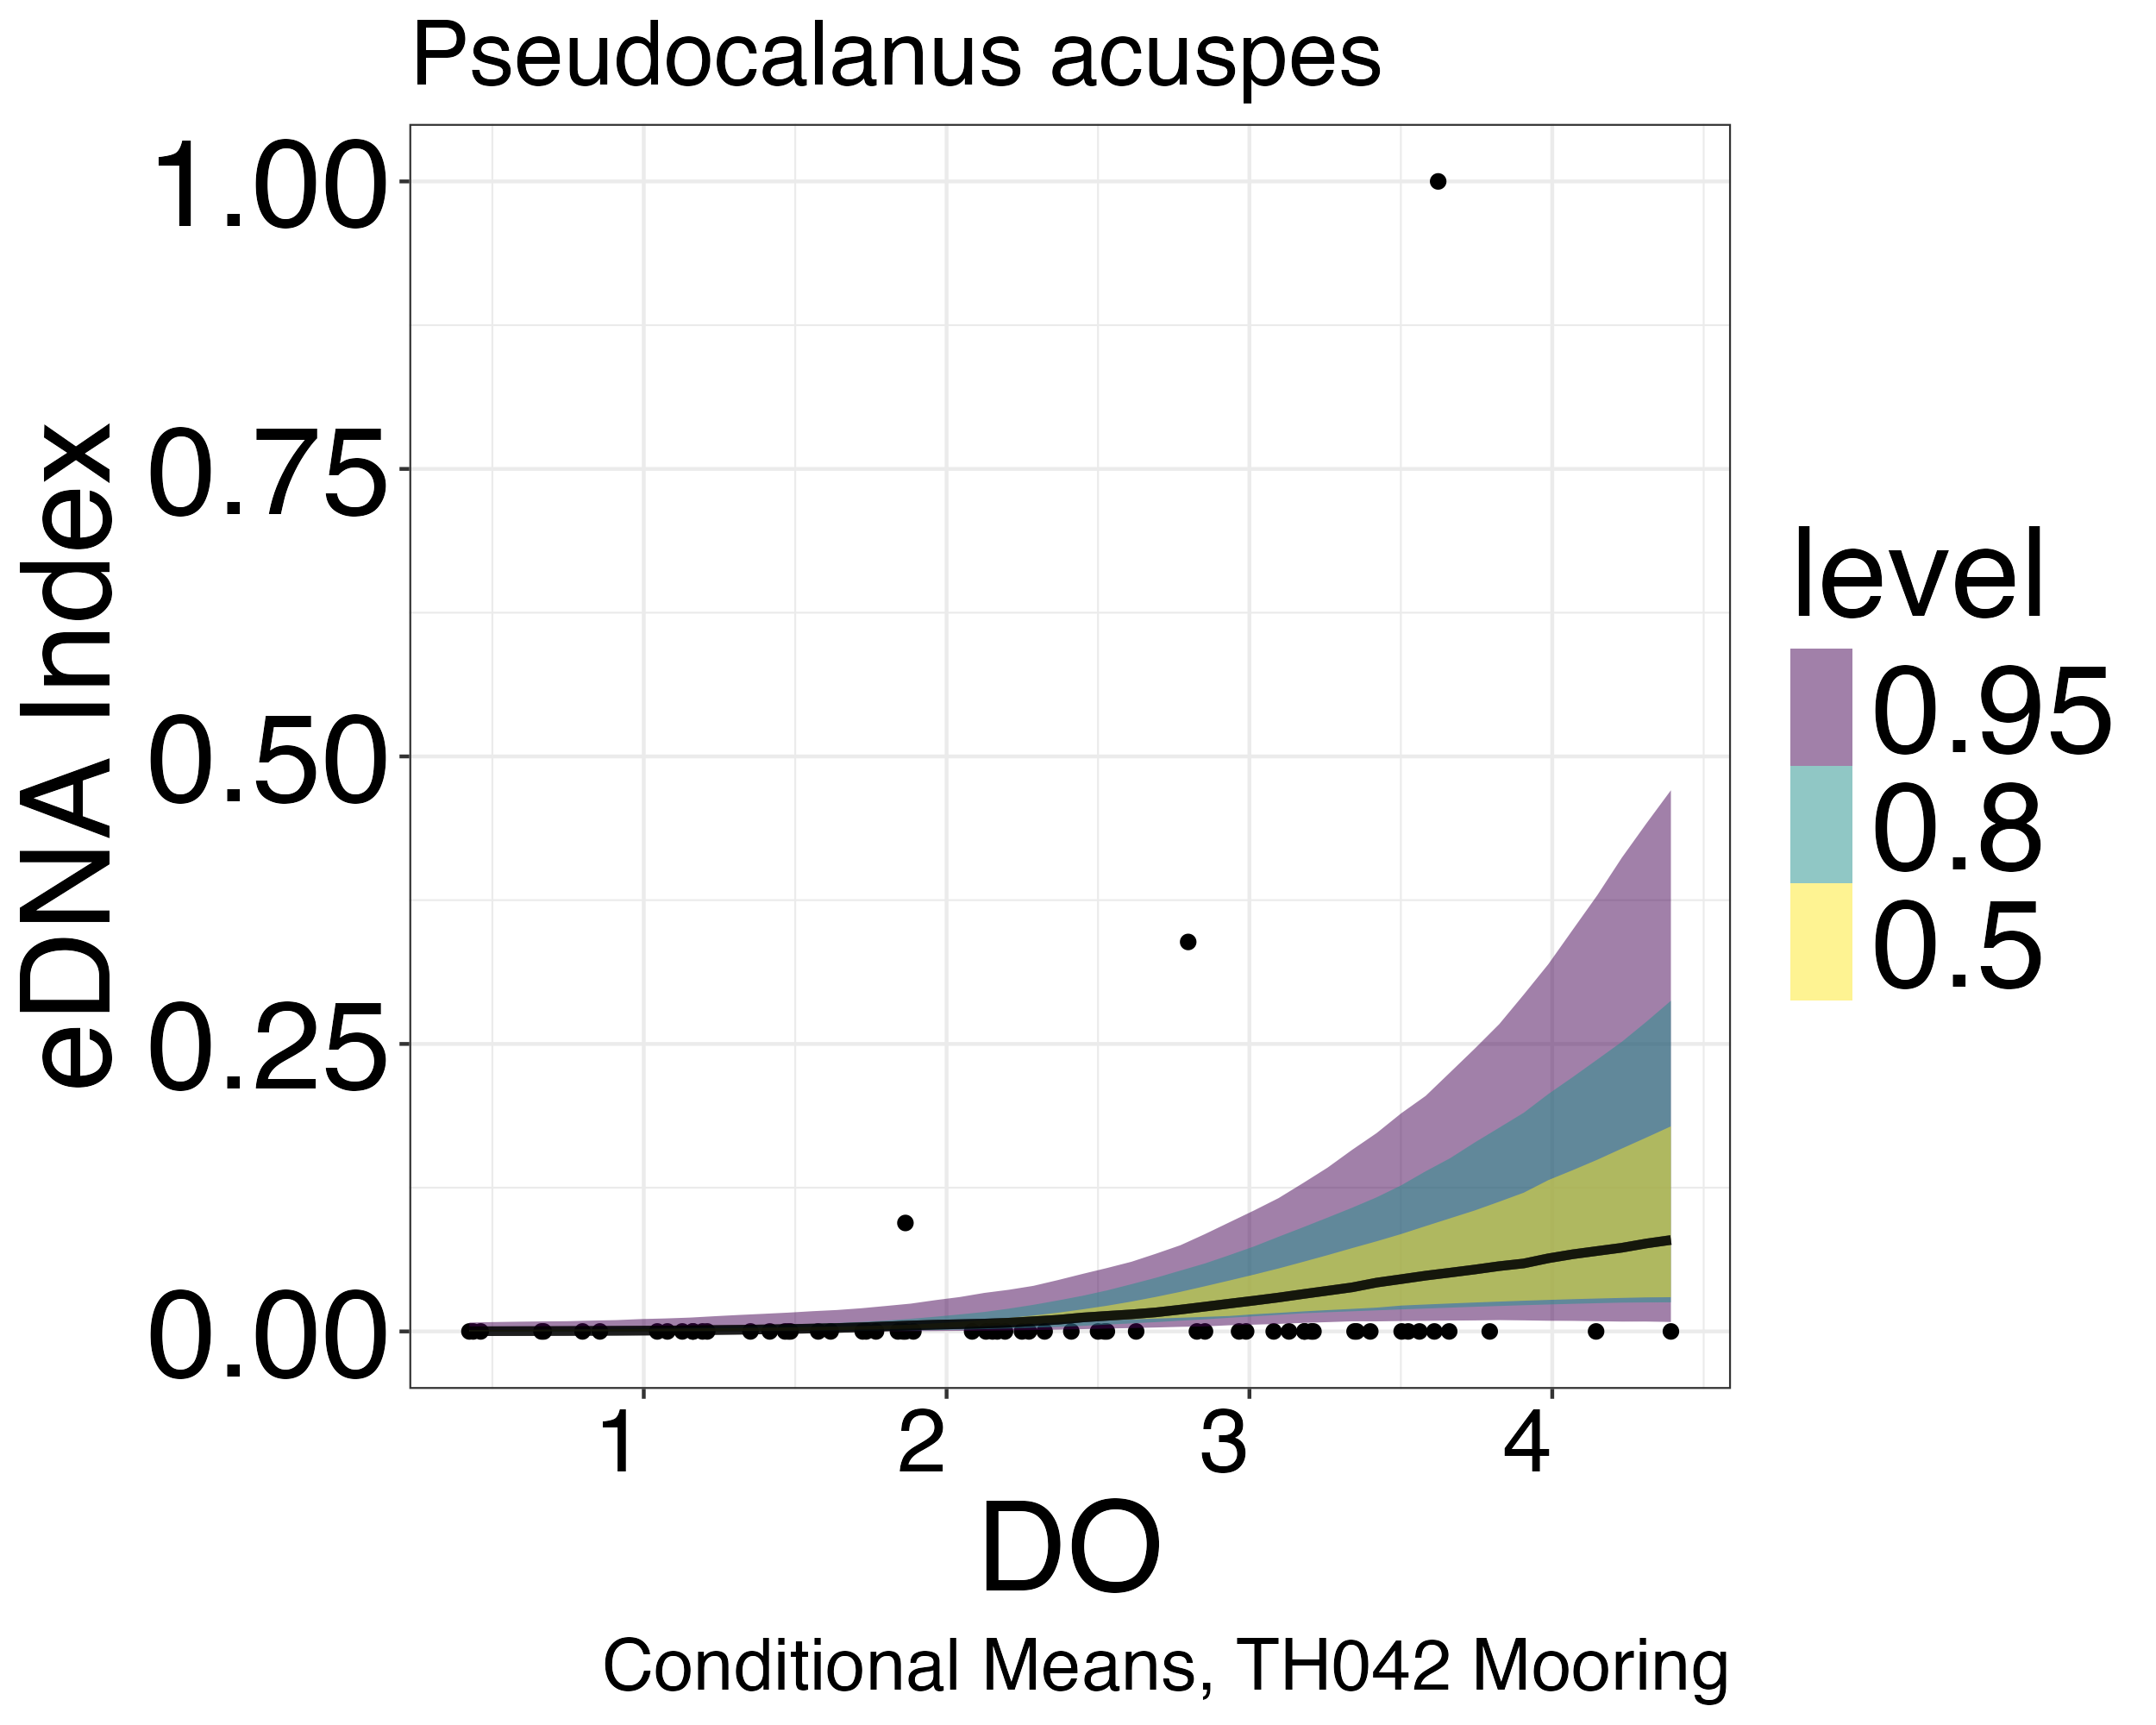
\includegraphics[scale=0.25]{Pacuspes_ZOIB_Means_noOut} \\
			Year-round: \\
			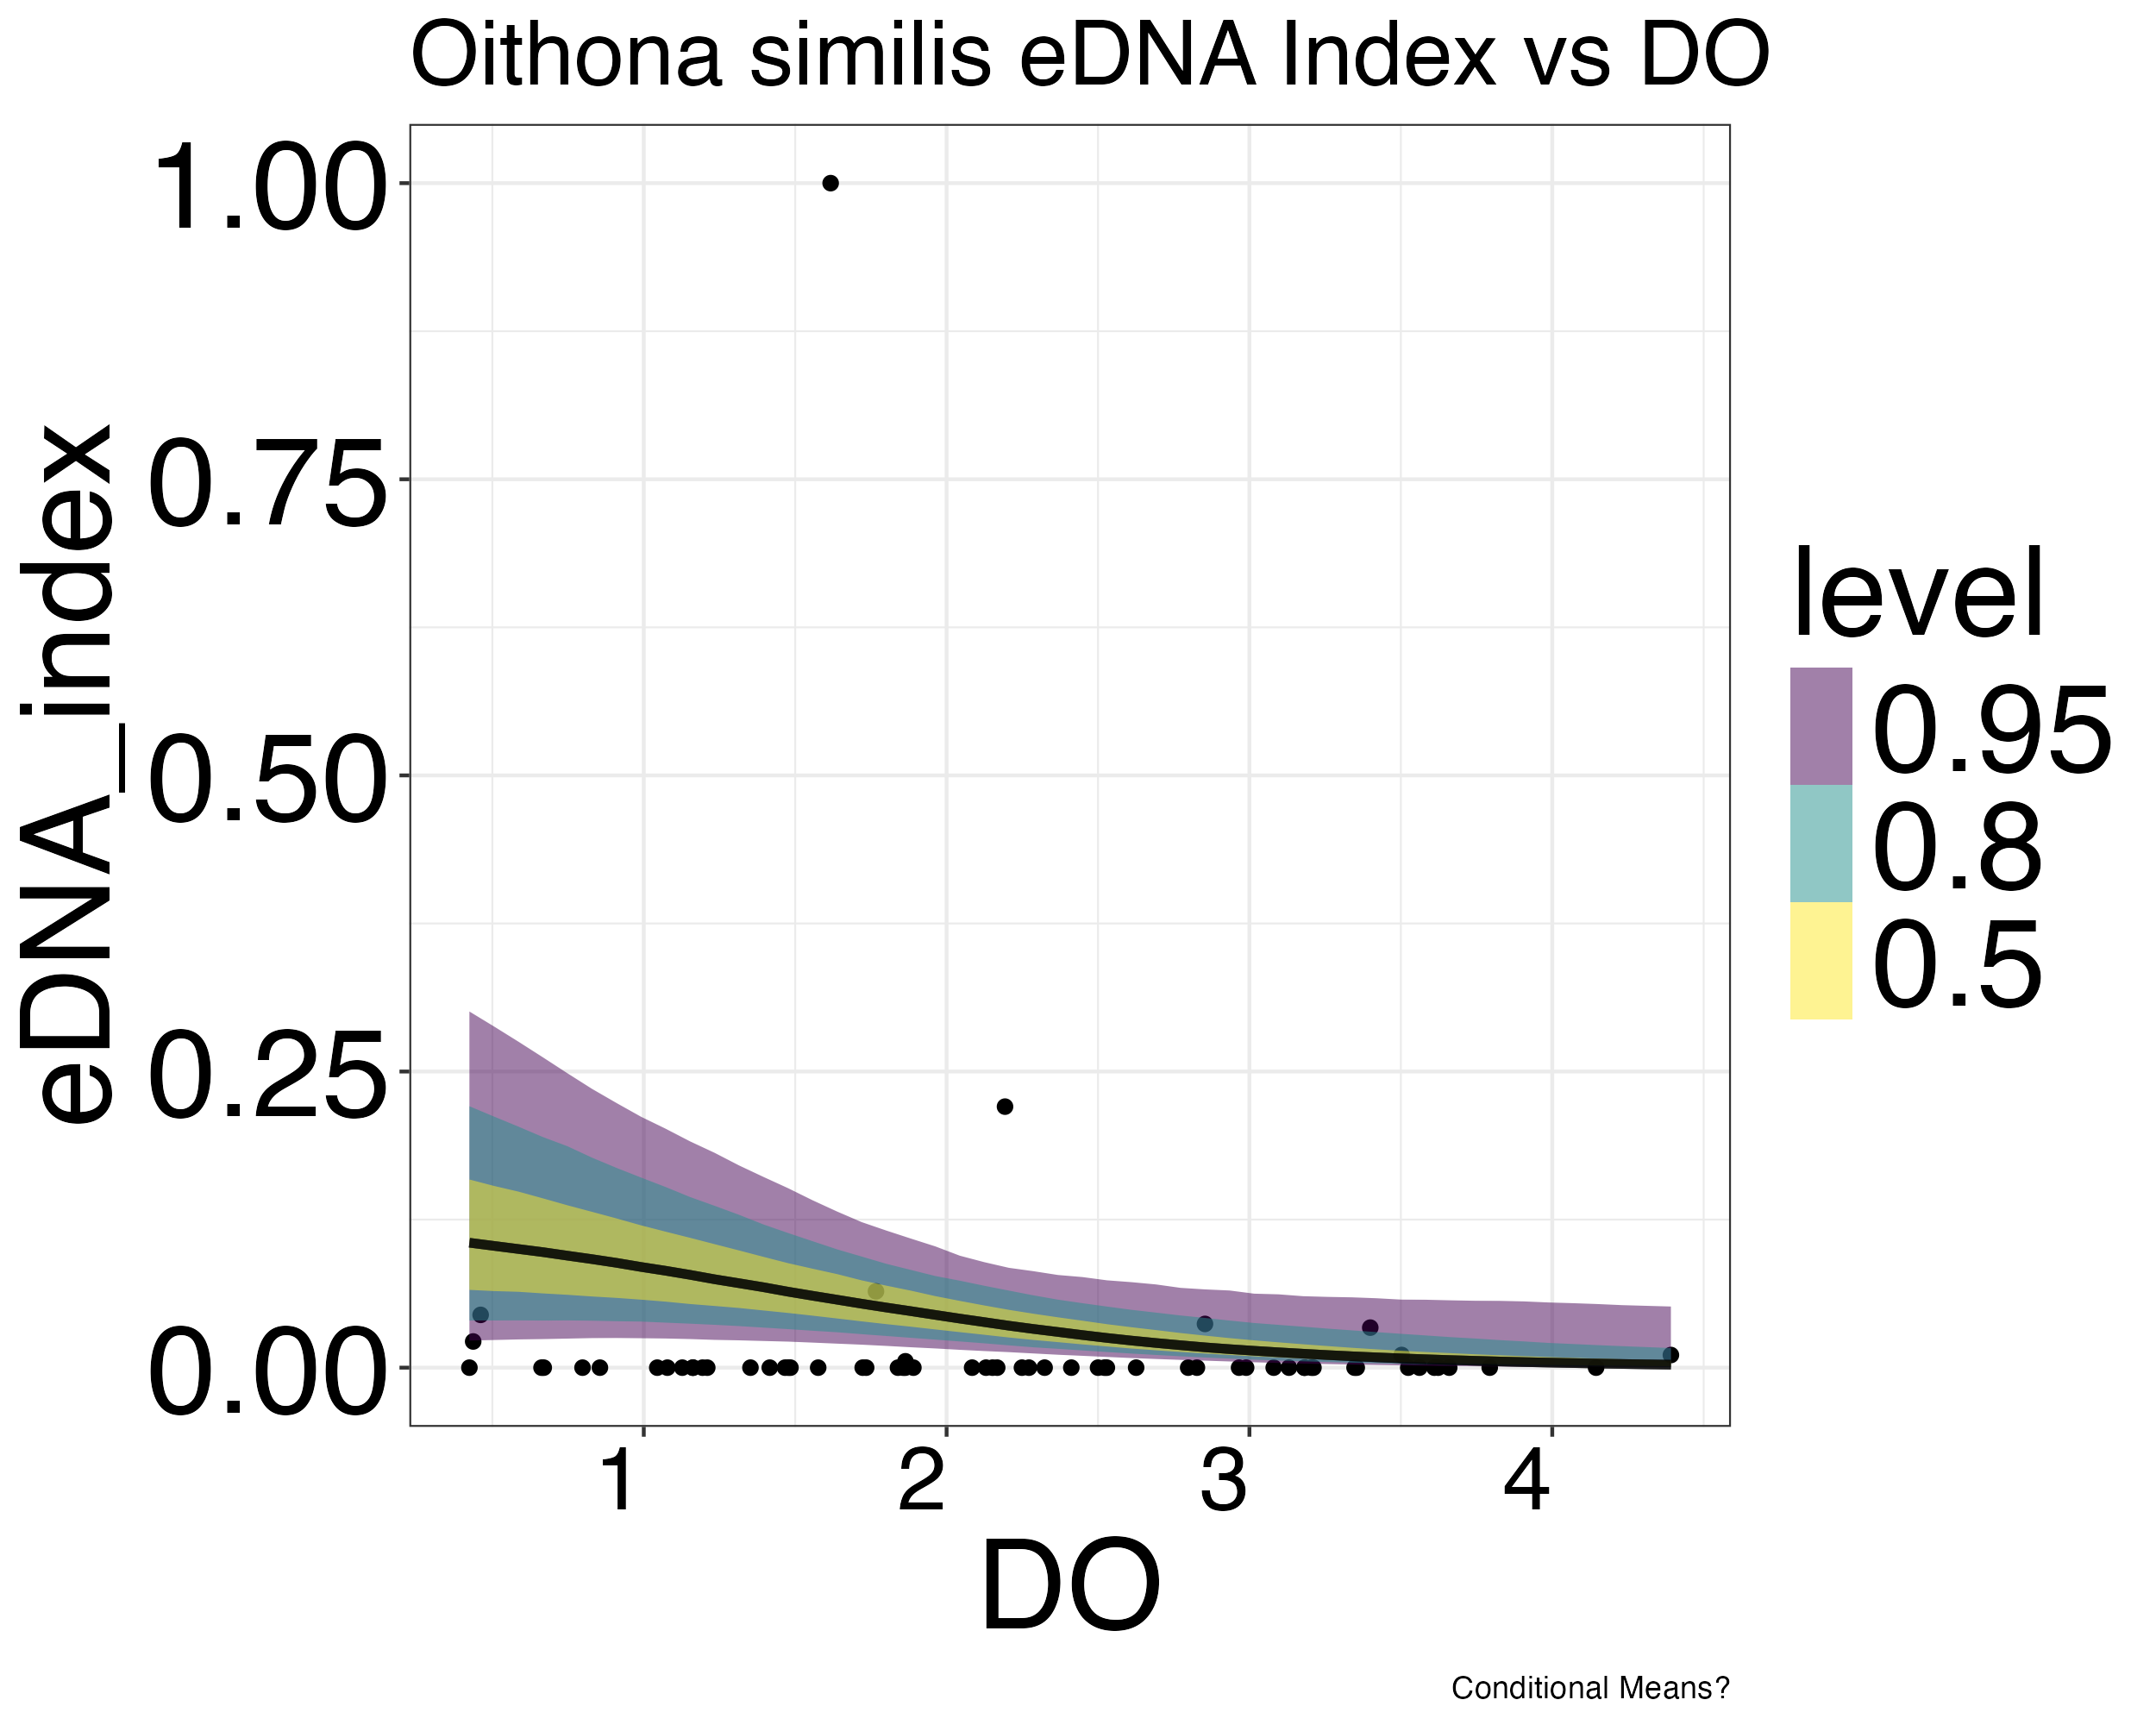
\includegraphics[scale=0.25]{Osimilis_ZOIB_Means_noOut} \\
			Southern: \\
			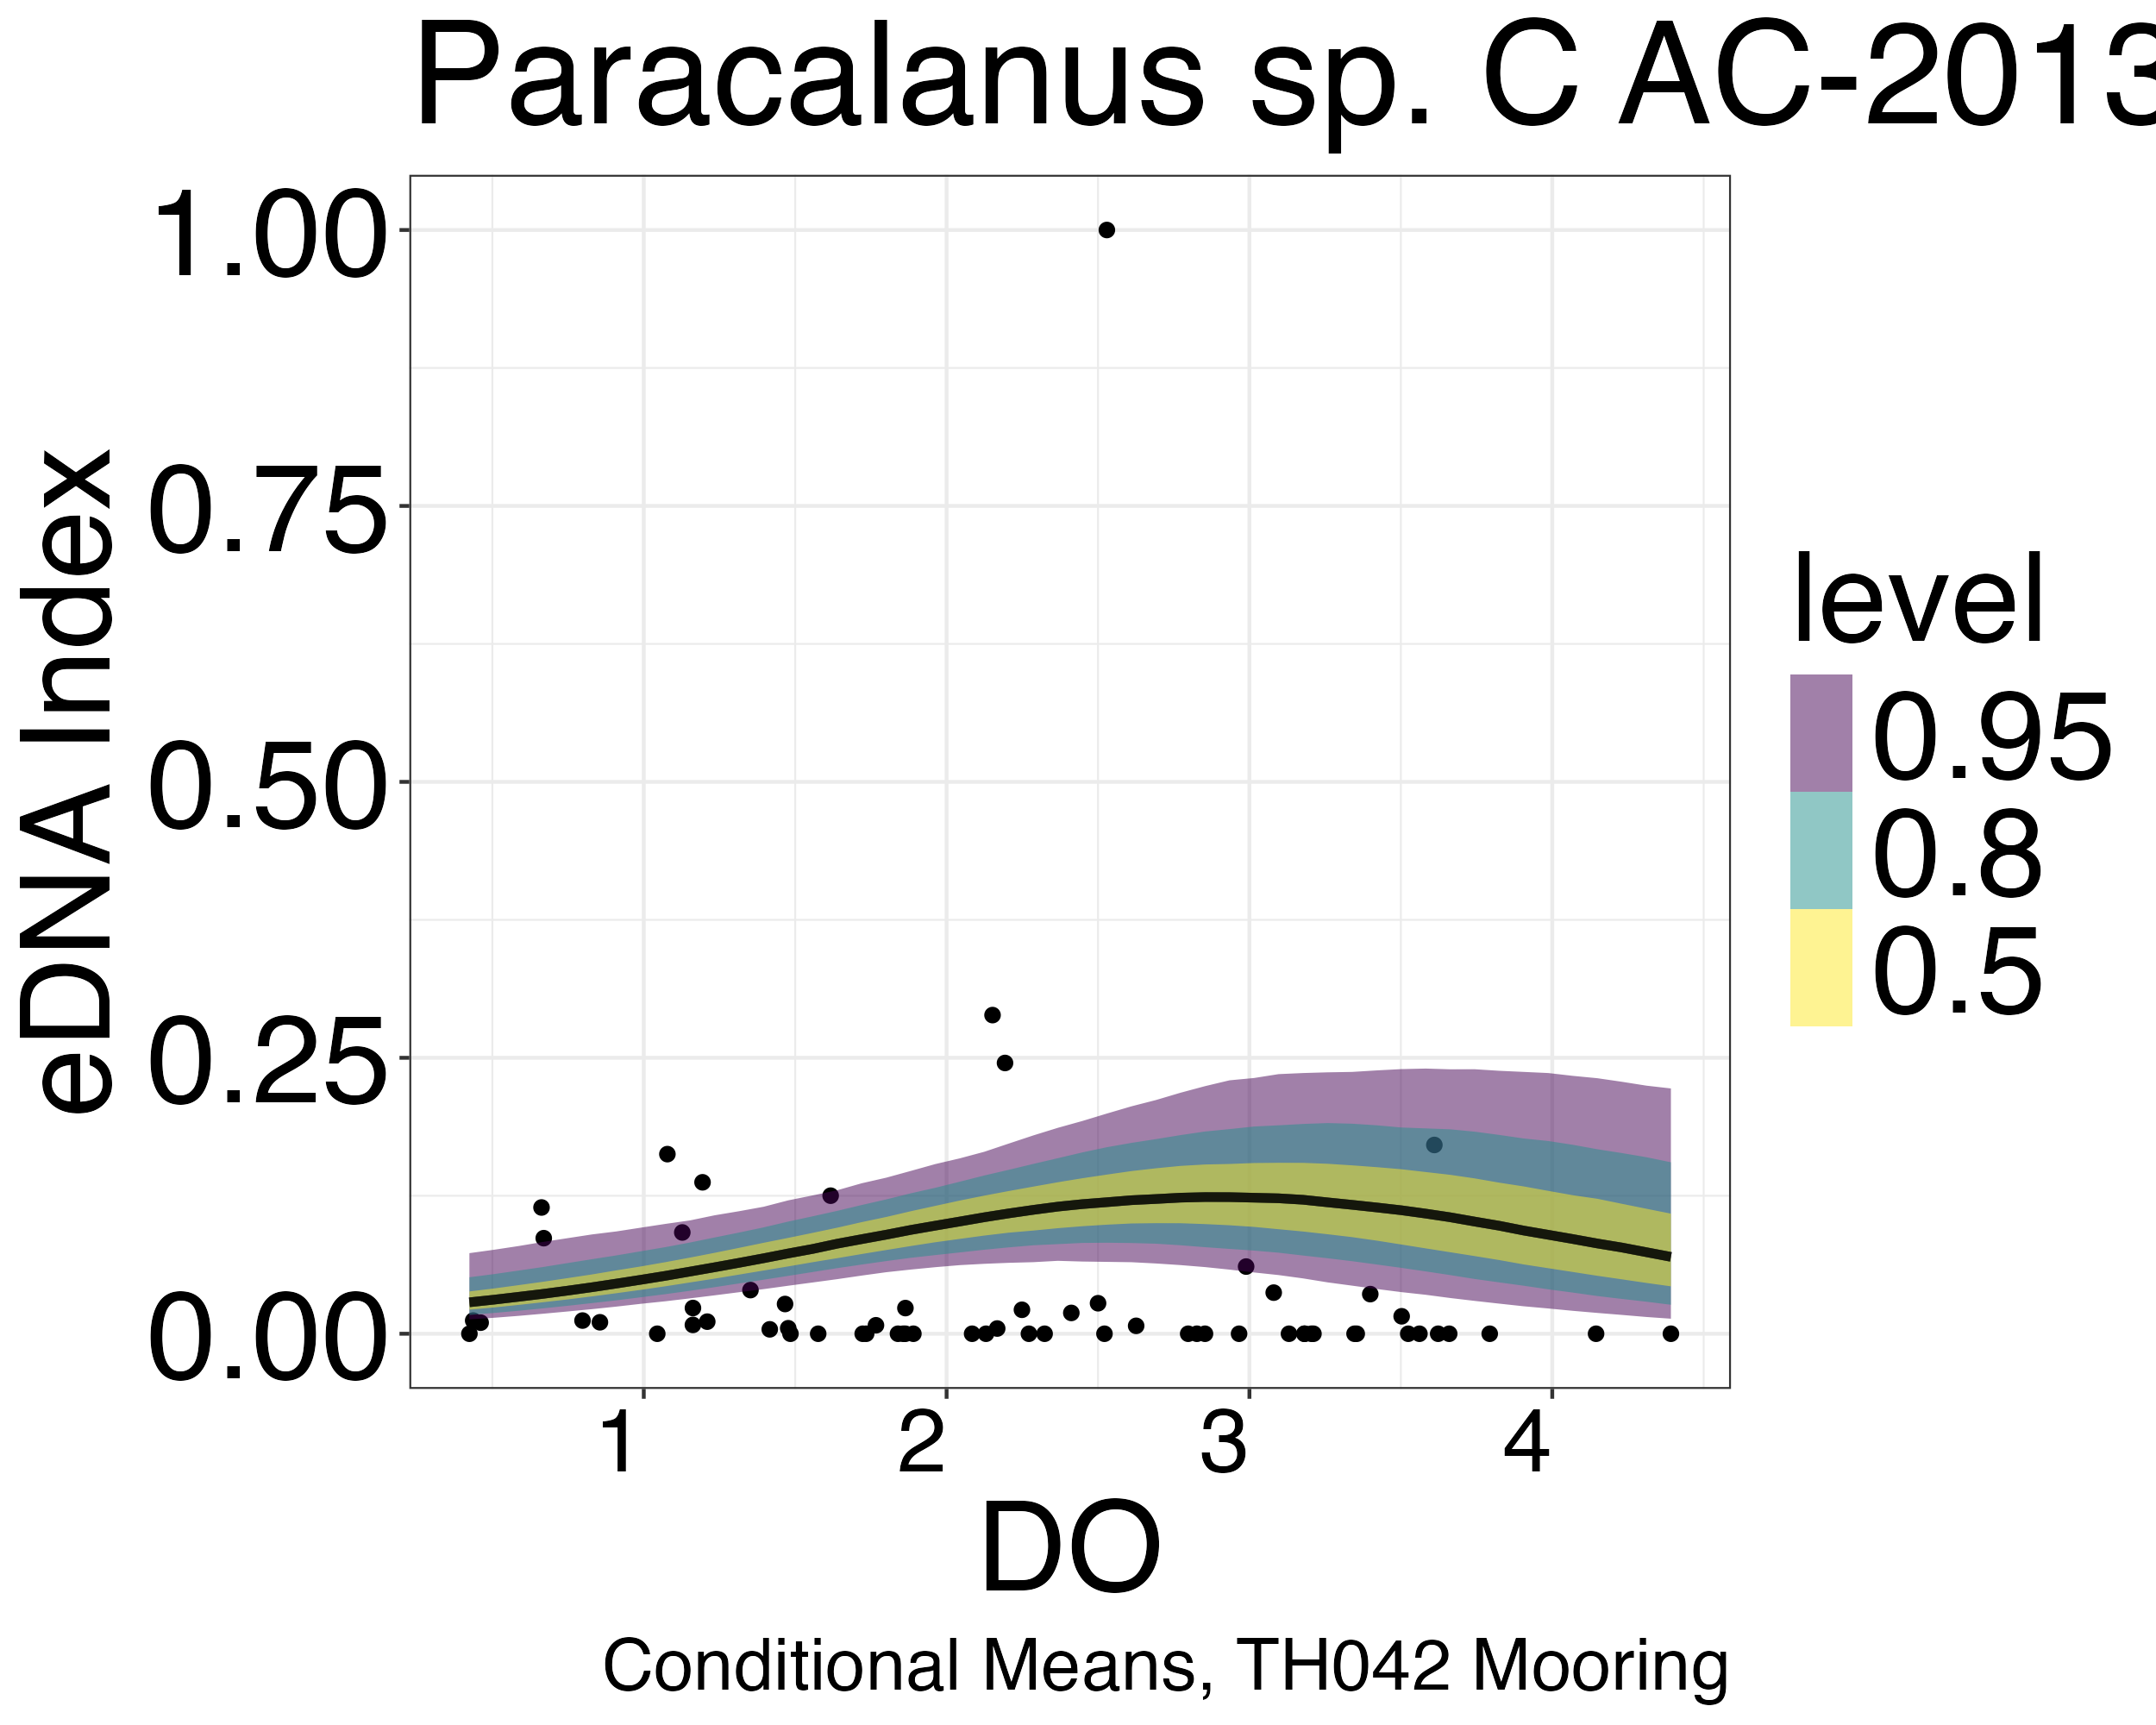
\includegraphics[scale=0.25]{Paracalanus_ZOIB_Means_noOut}
			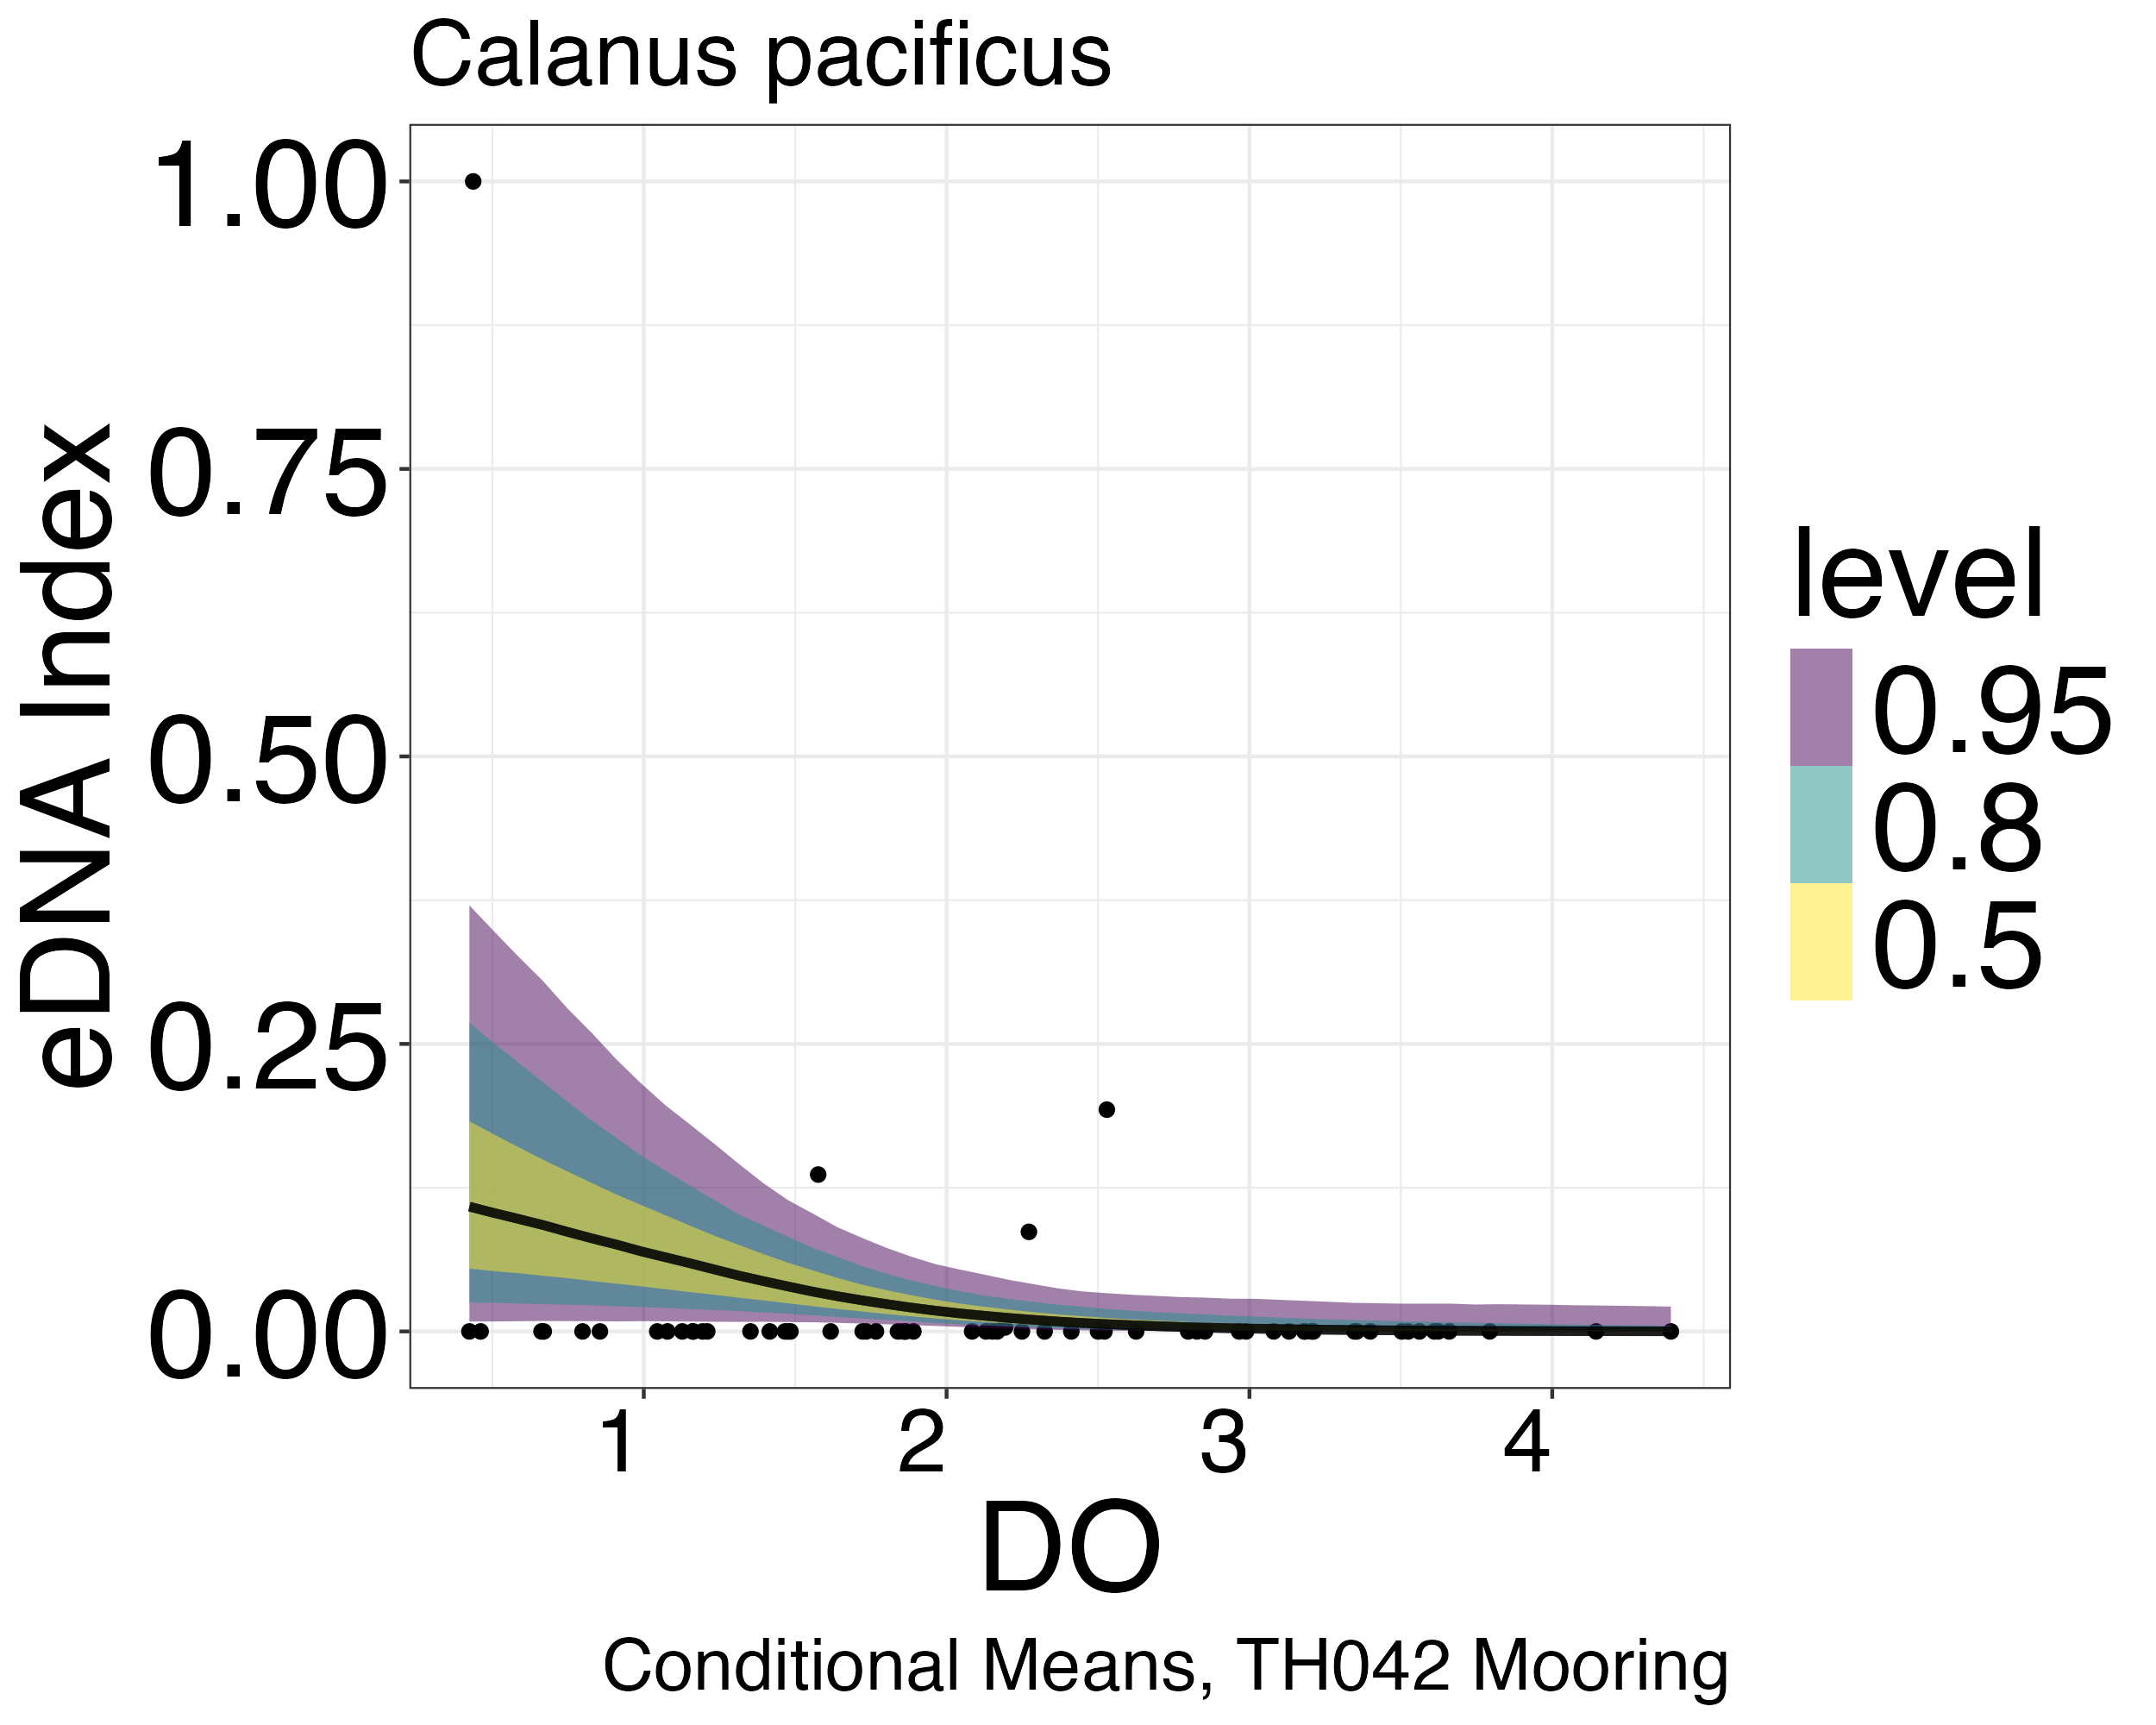
\includegraphics[scale=0.25]{Cpacificus_ZOIB_Means_noOut}
			\caption[Zero-inflated beta regression means]{\footnotesize{Zero-inflated beta regression model means, with bands showing 0.5, 0.8, and 0.95 confidence levels, using data from 2021-22 from the TH042 mooring.}} %the special ToC caption is in square brackets. The \footnotesize makes the figure caption smaller
			\label{ZOIB}
		\end{center}
	\end{figure}
	
	\begin{figure}[h]
		\begin{center}
			Northern: \\
			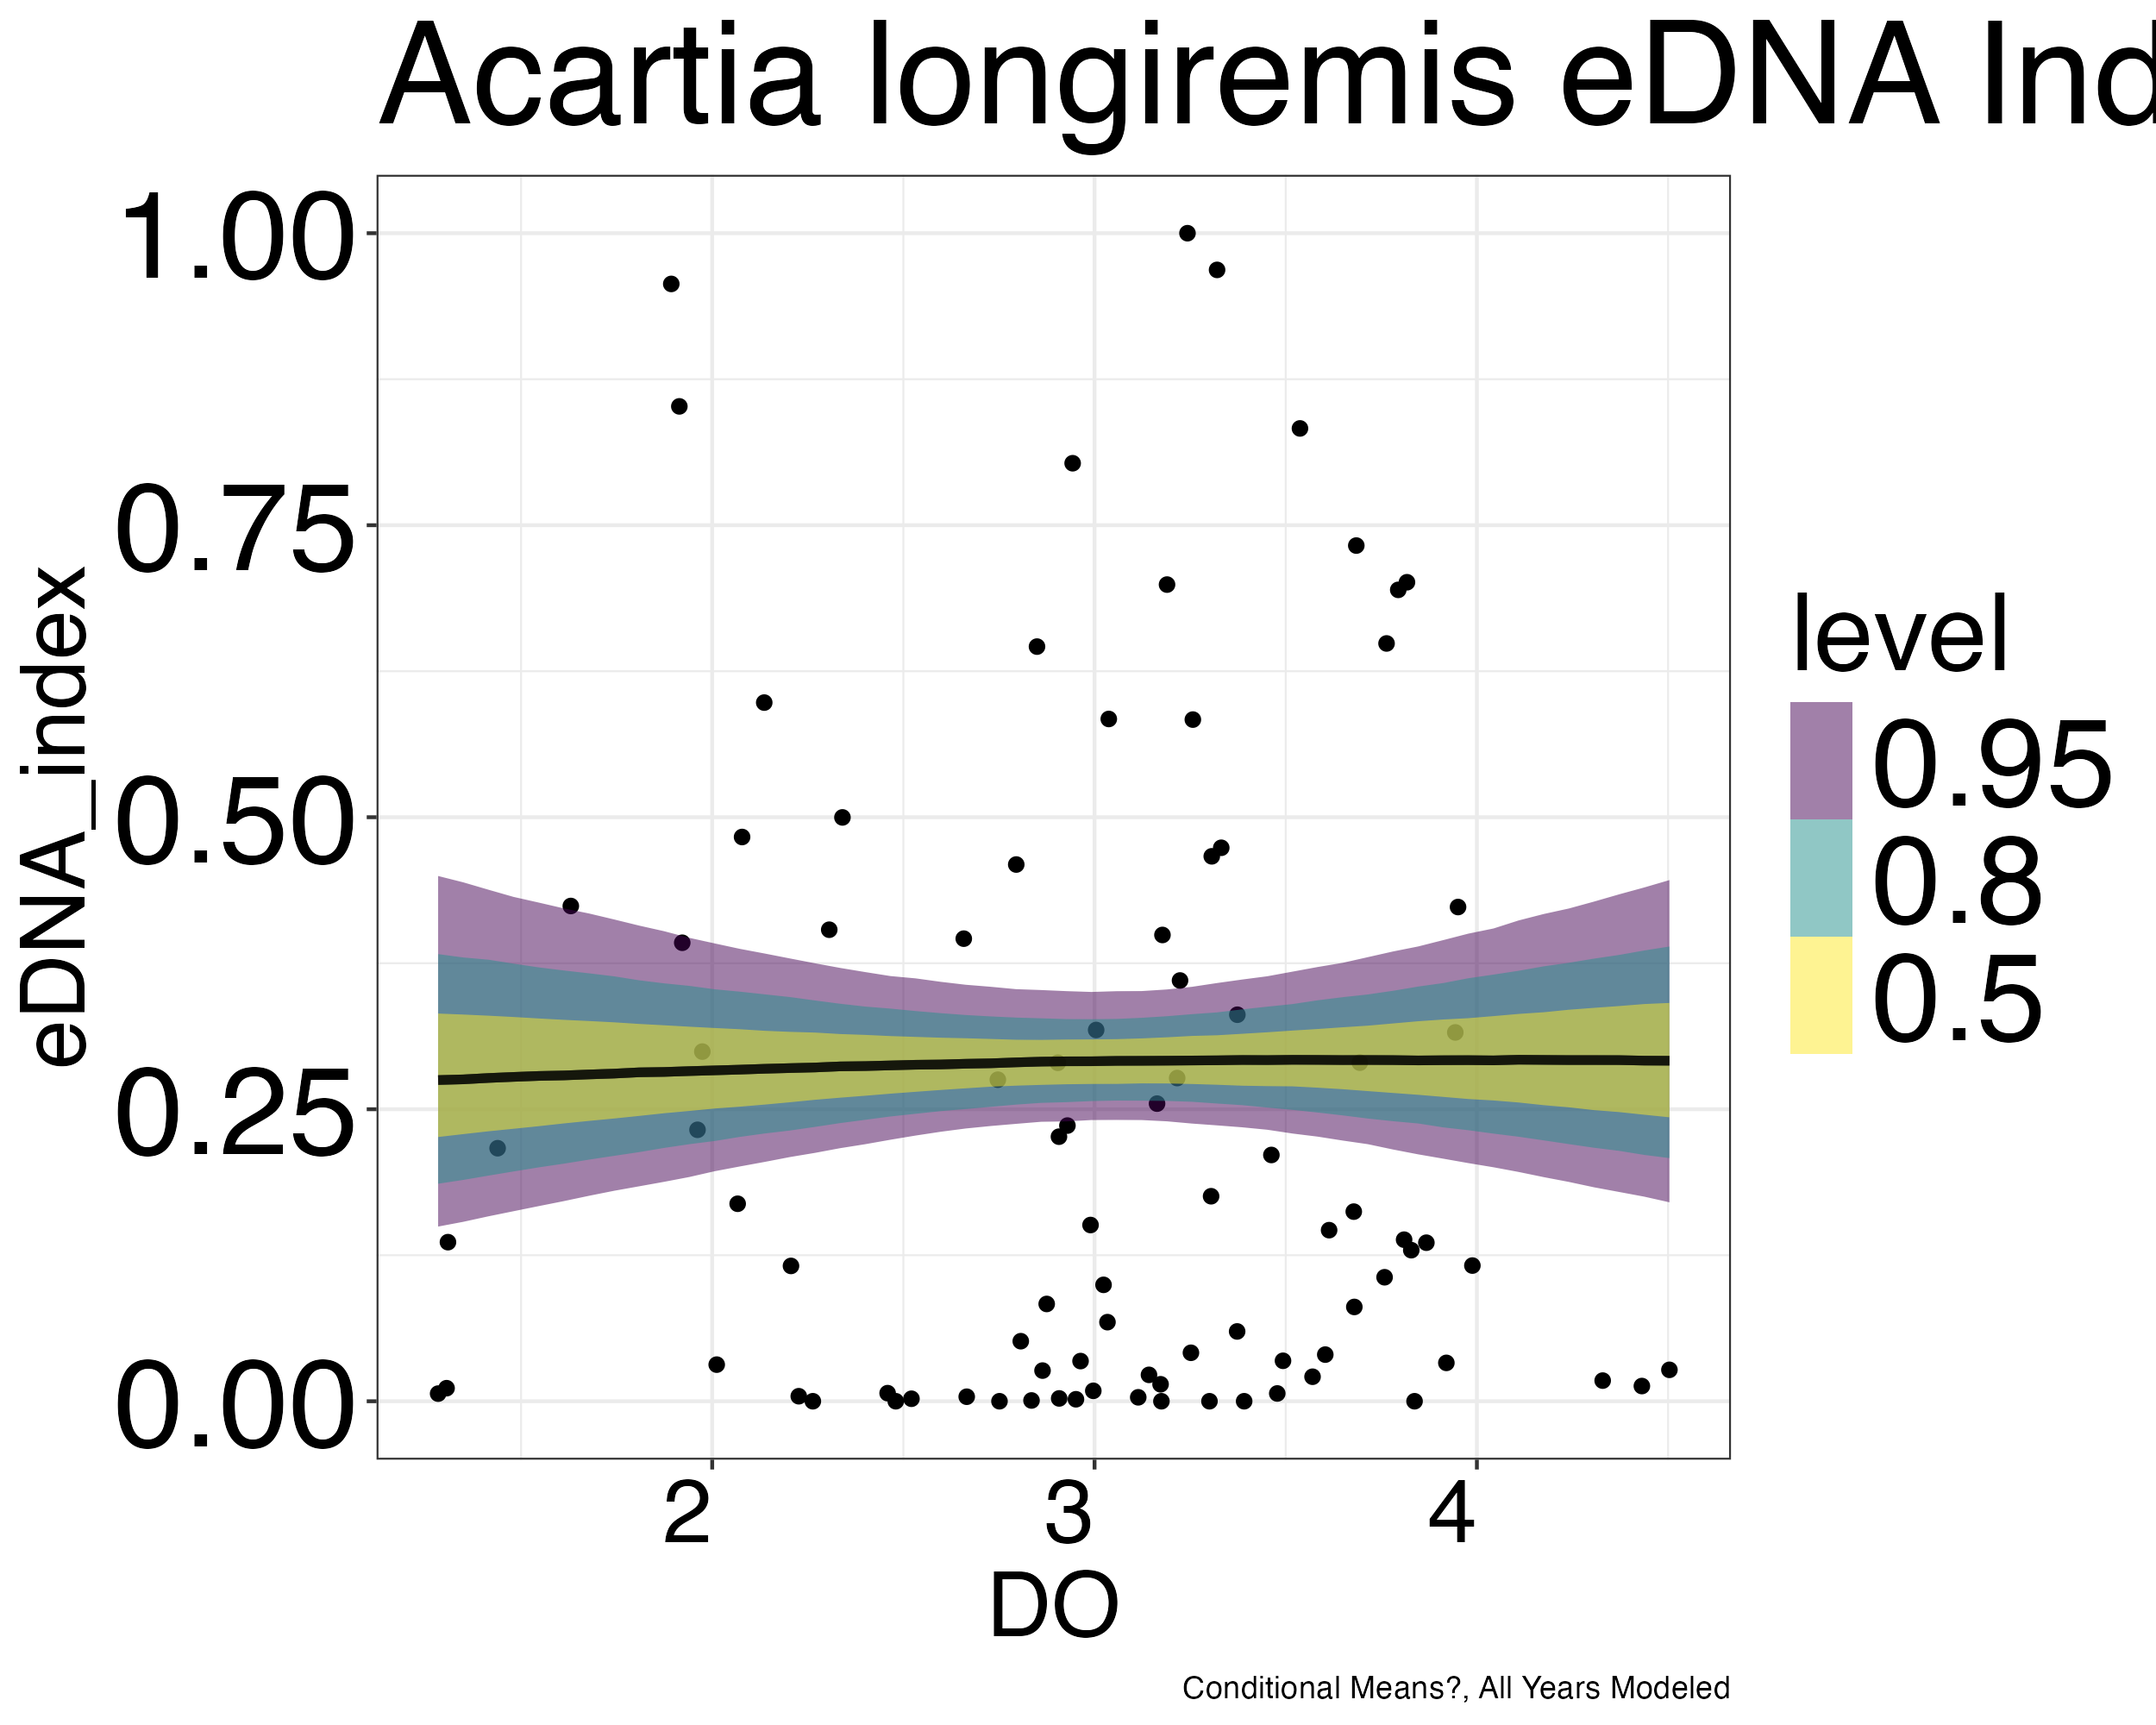
\includegraphics[scale=0.25]{Alongiremis_ZOIB_Means_Mod_noOut}
			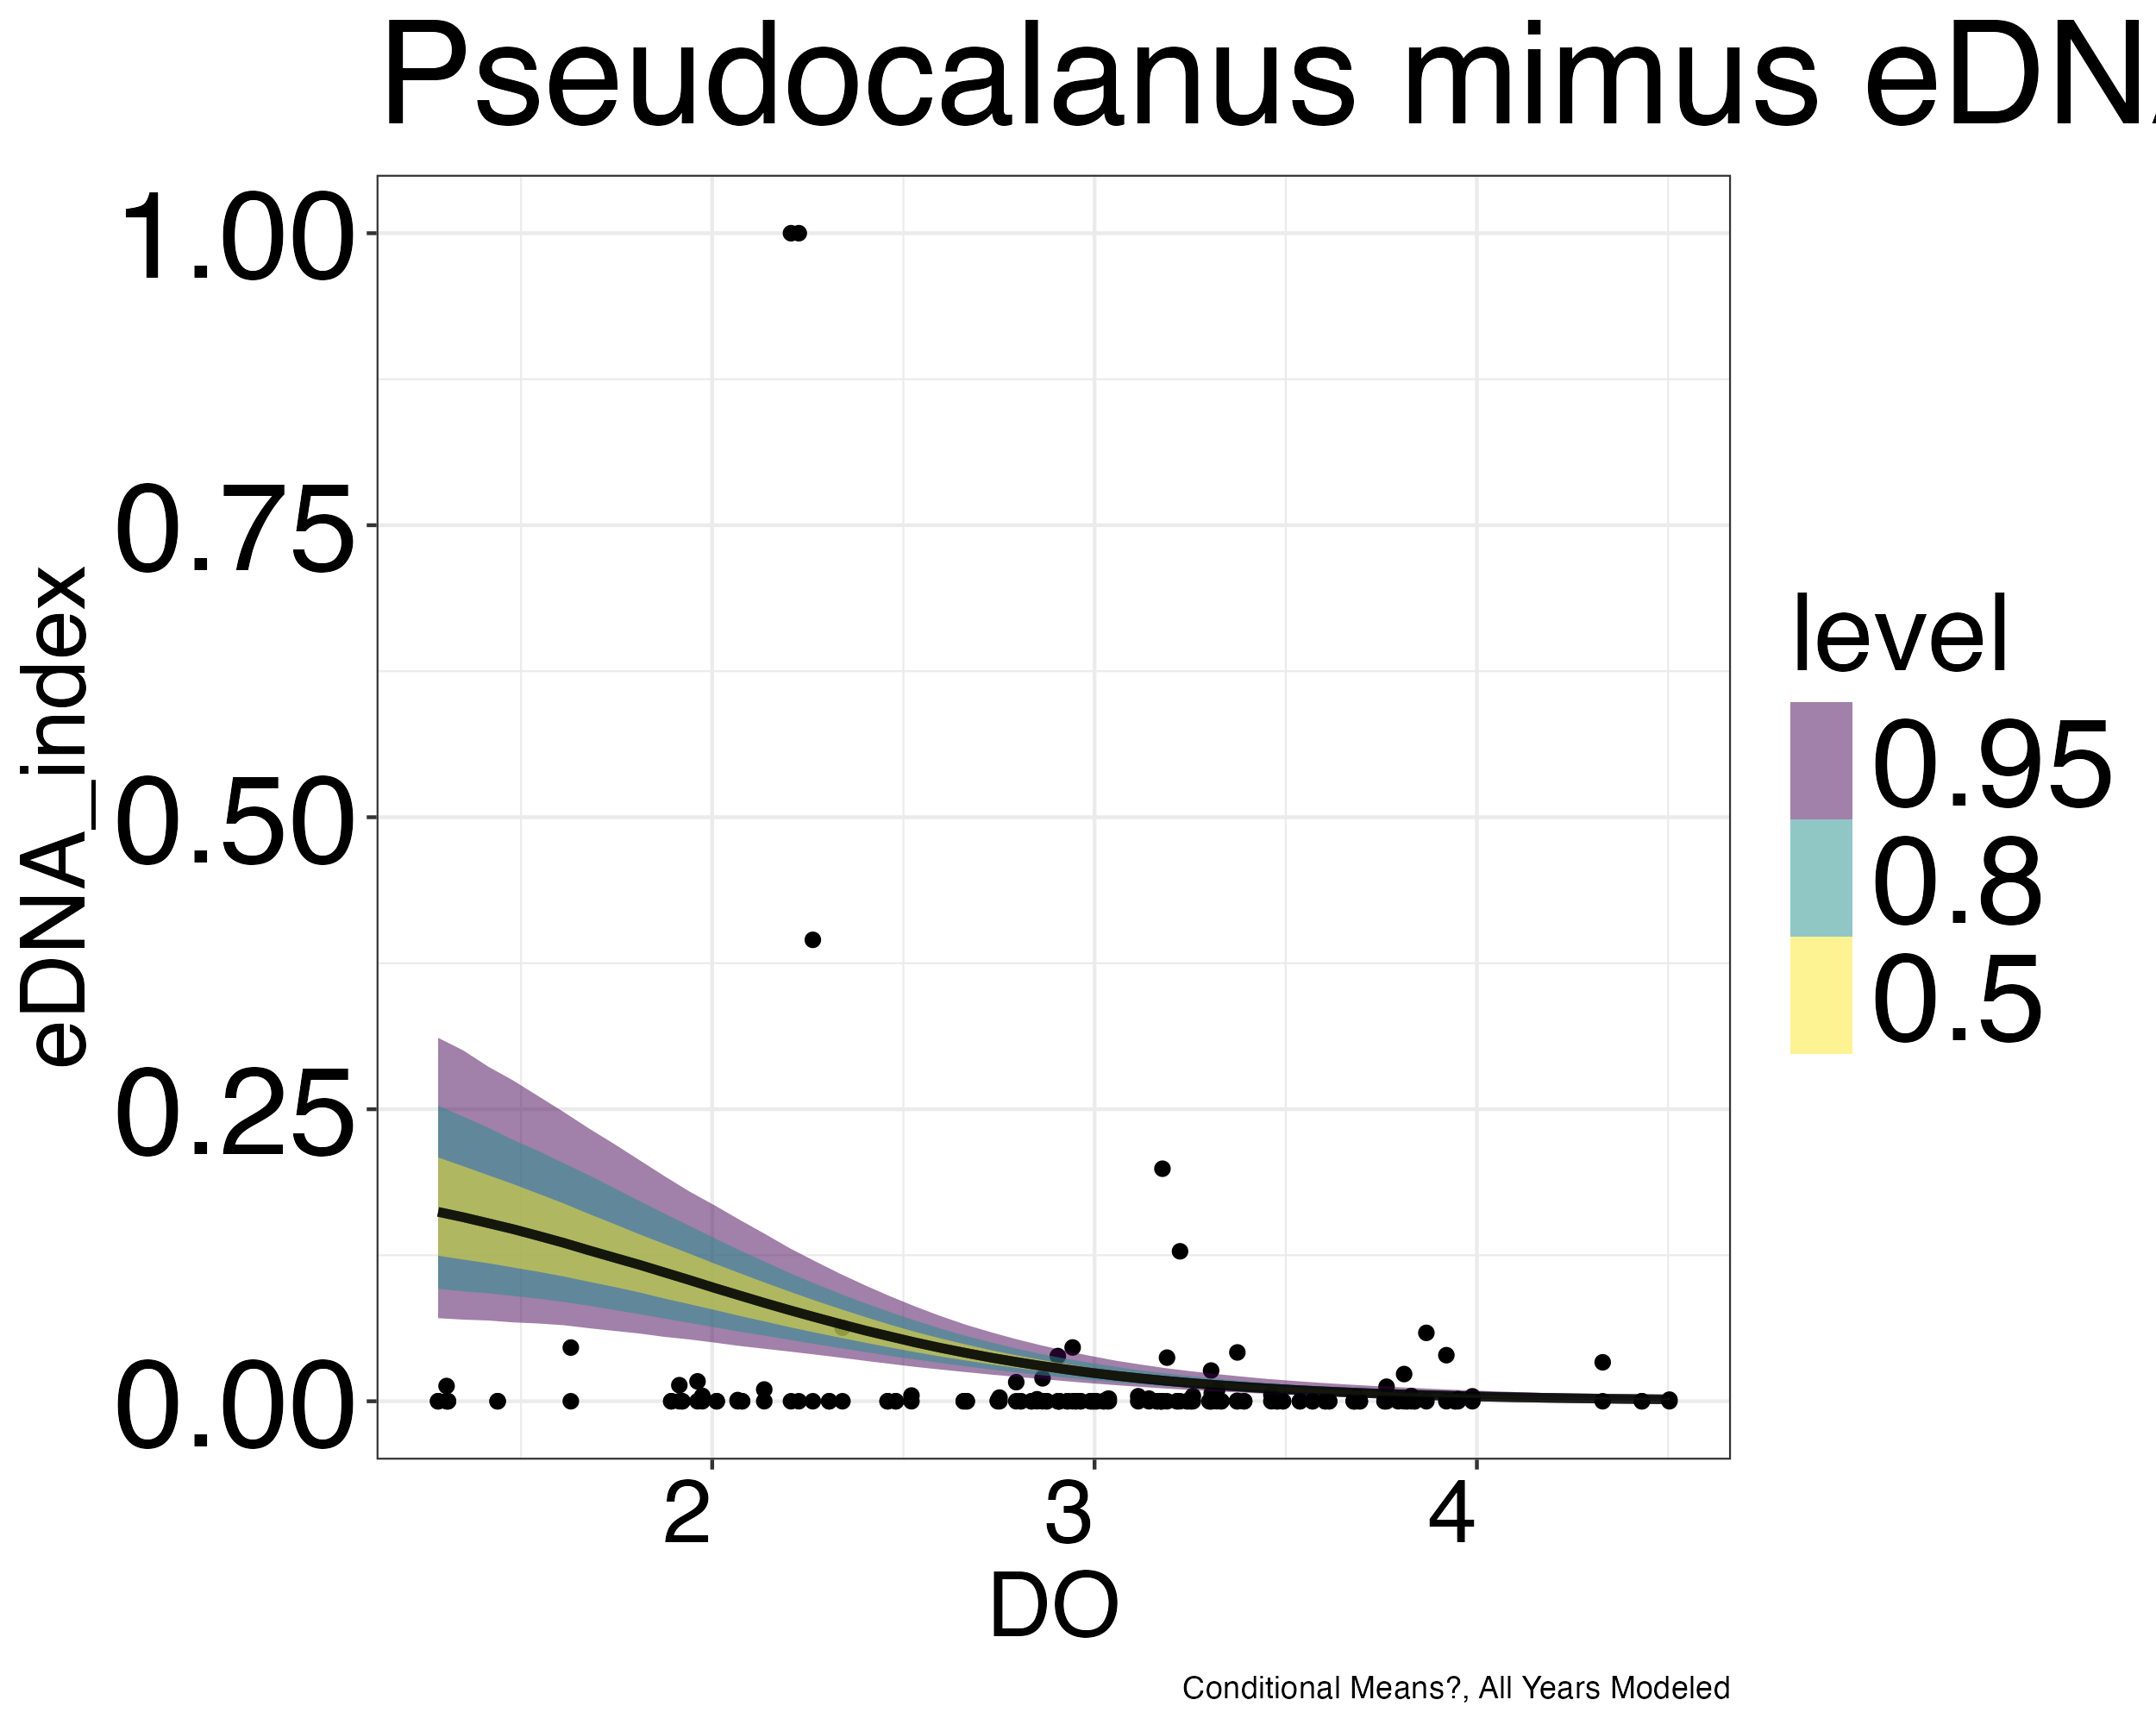
\includegraphics[scale=0.25]{Pmimus_ZOIB_Means_Mod_noOut}
			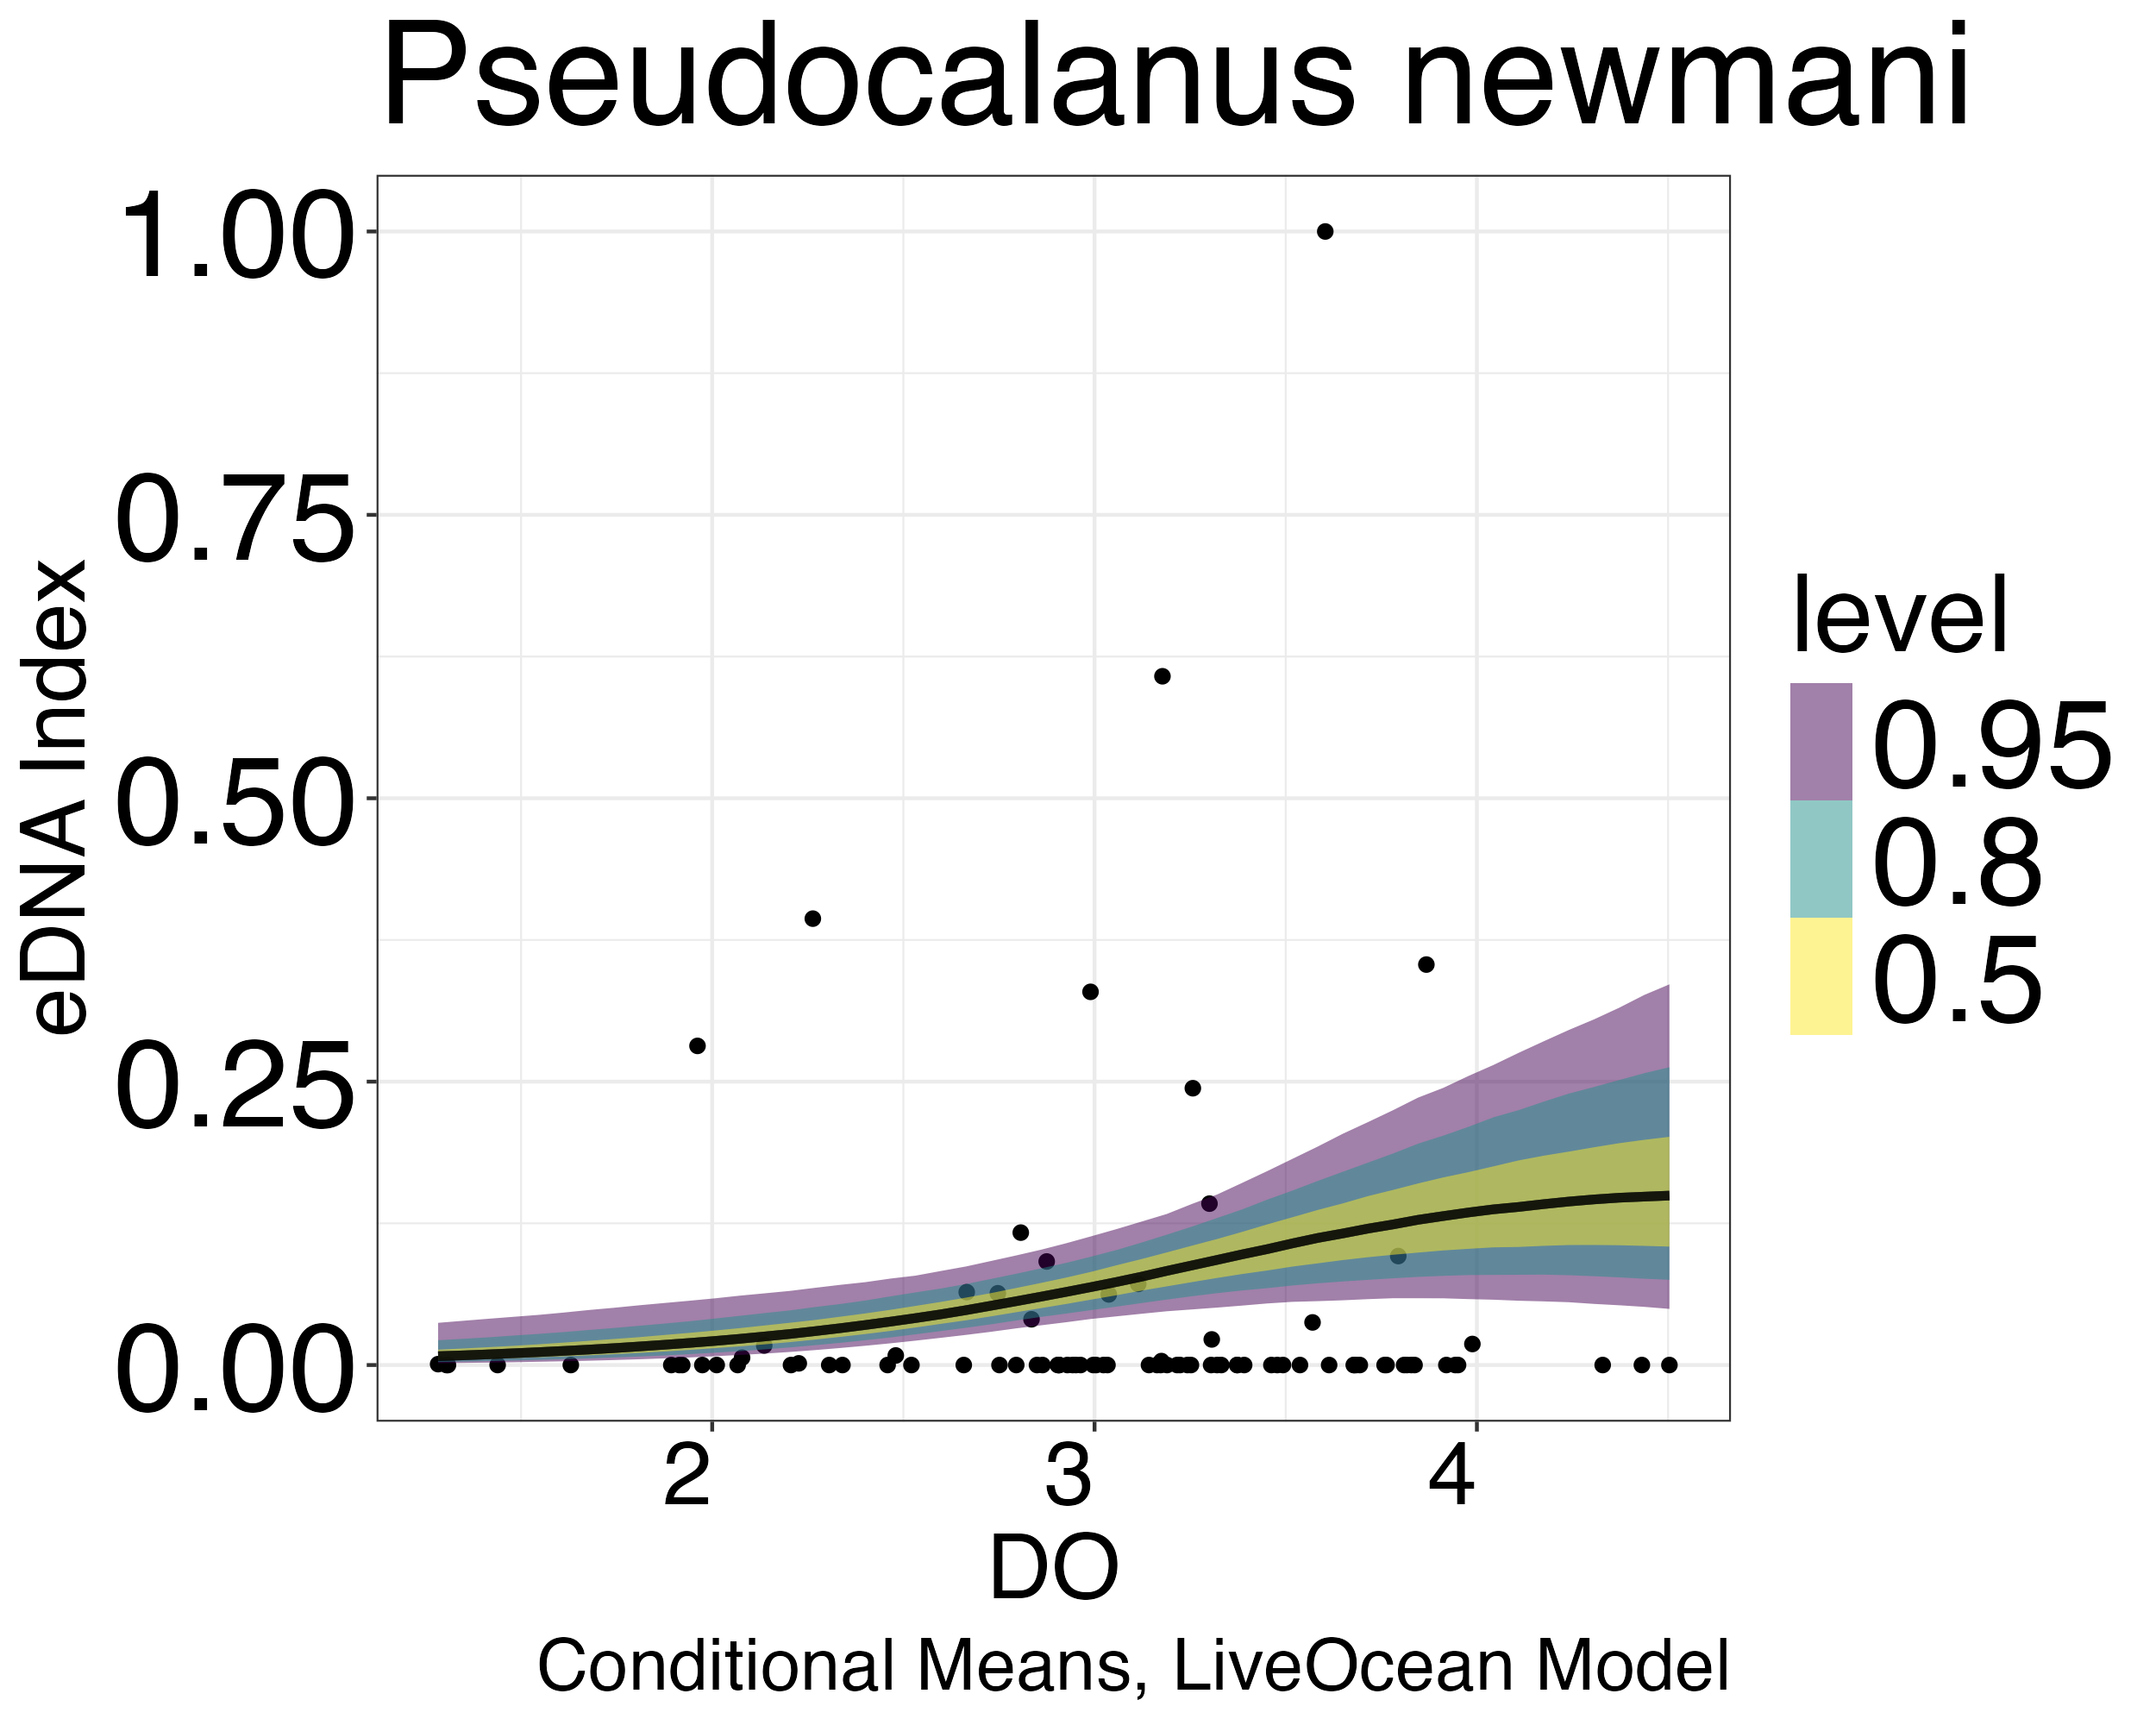
\includegraphics[scale=0.25]{Pnewmani_ZOIB_Means_Mod_noOut}
			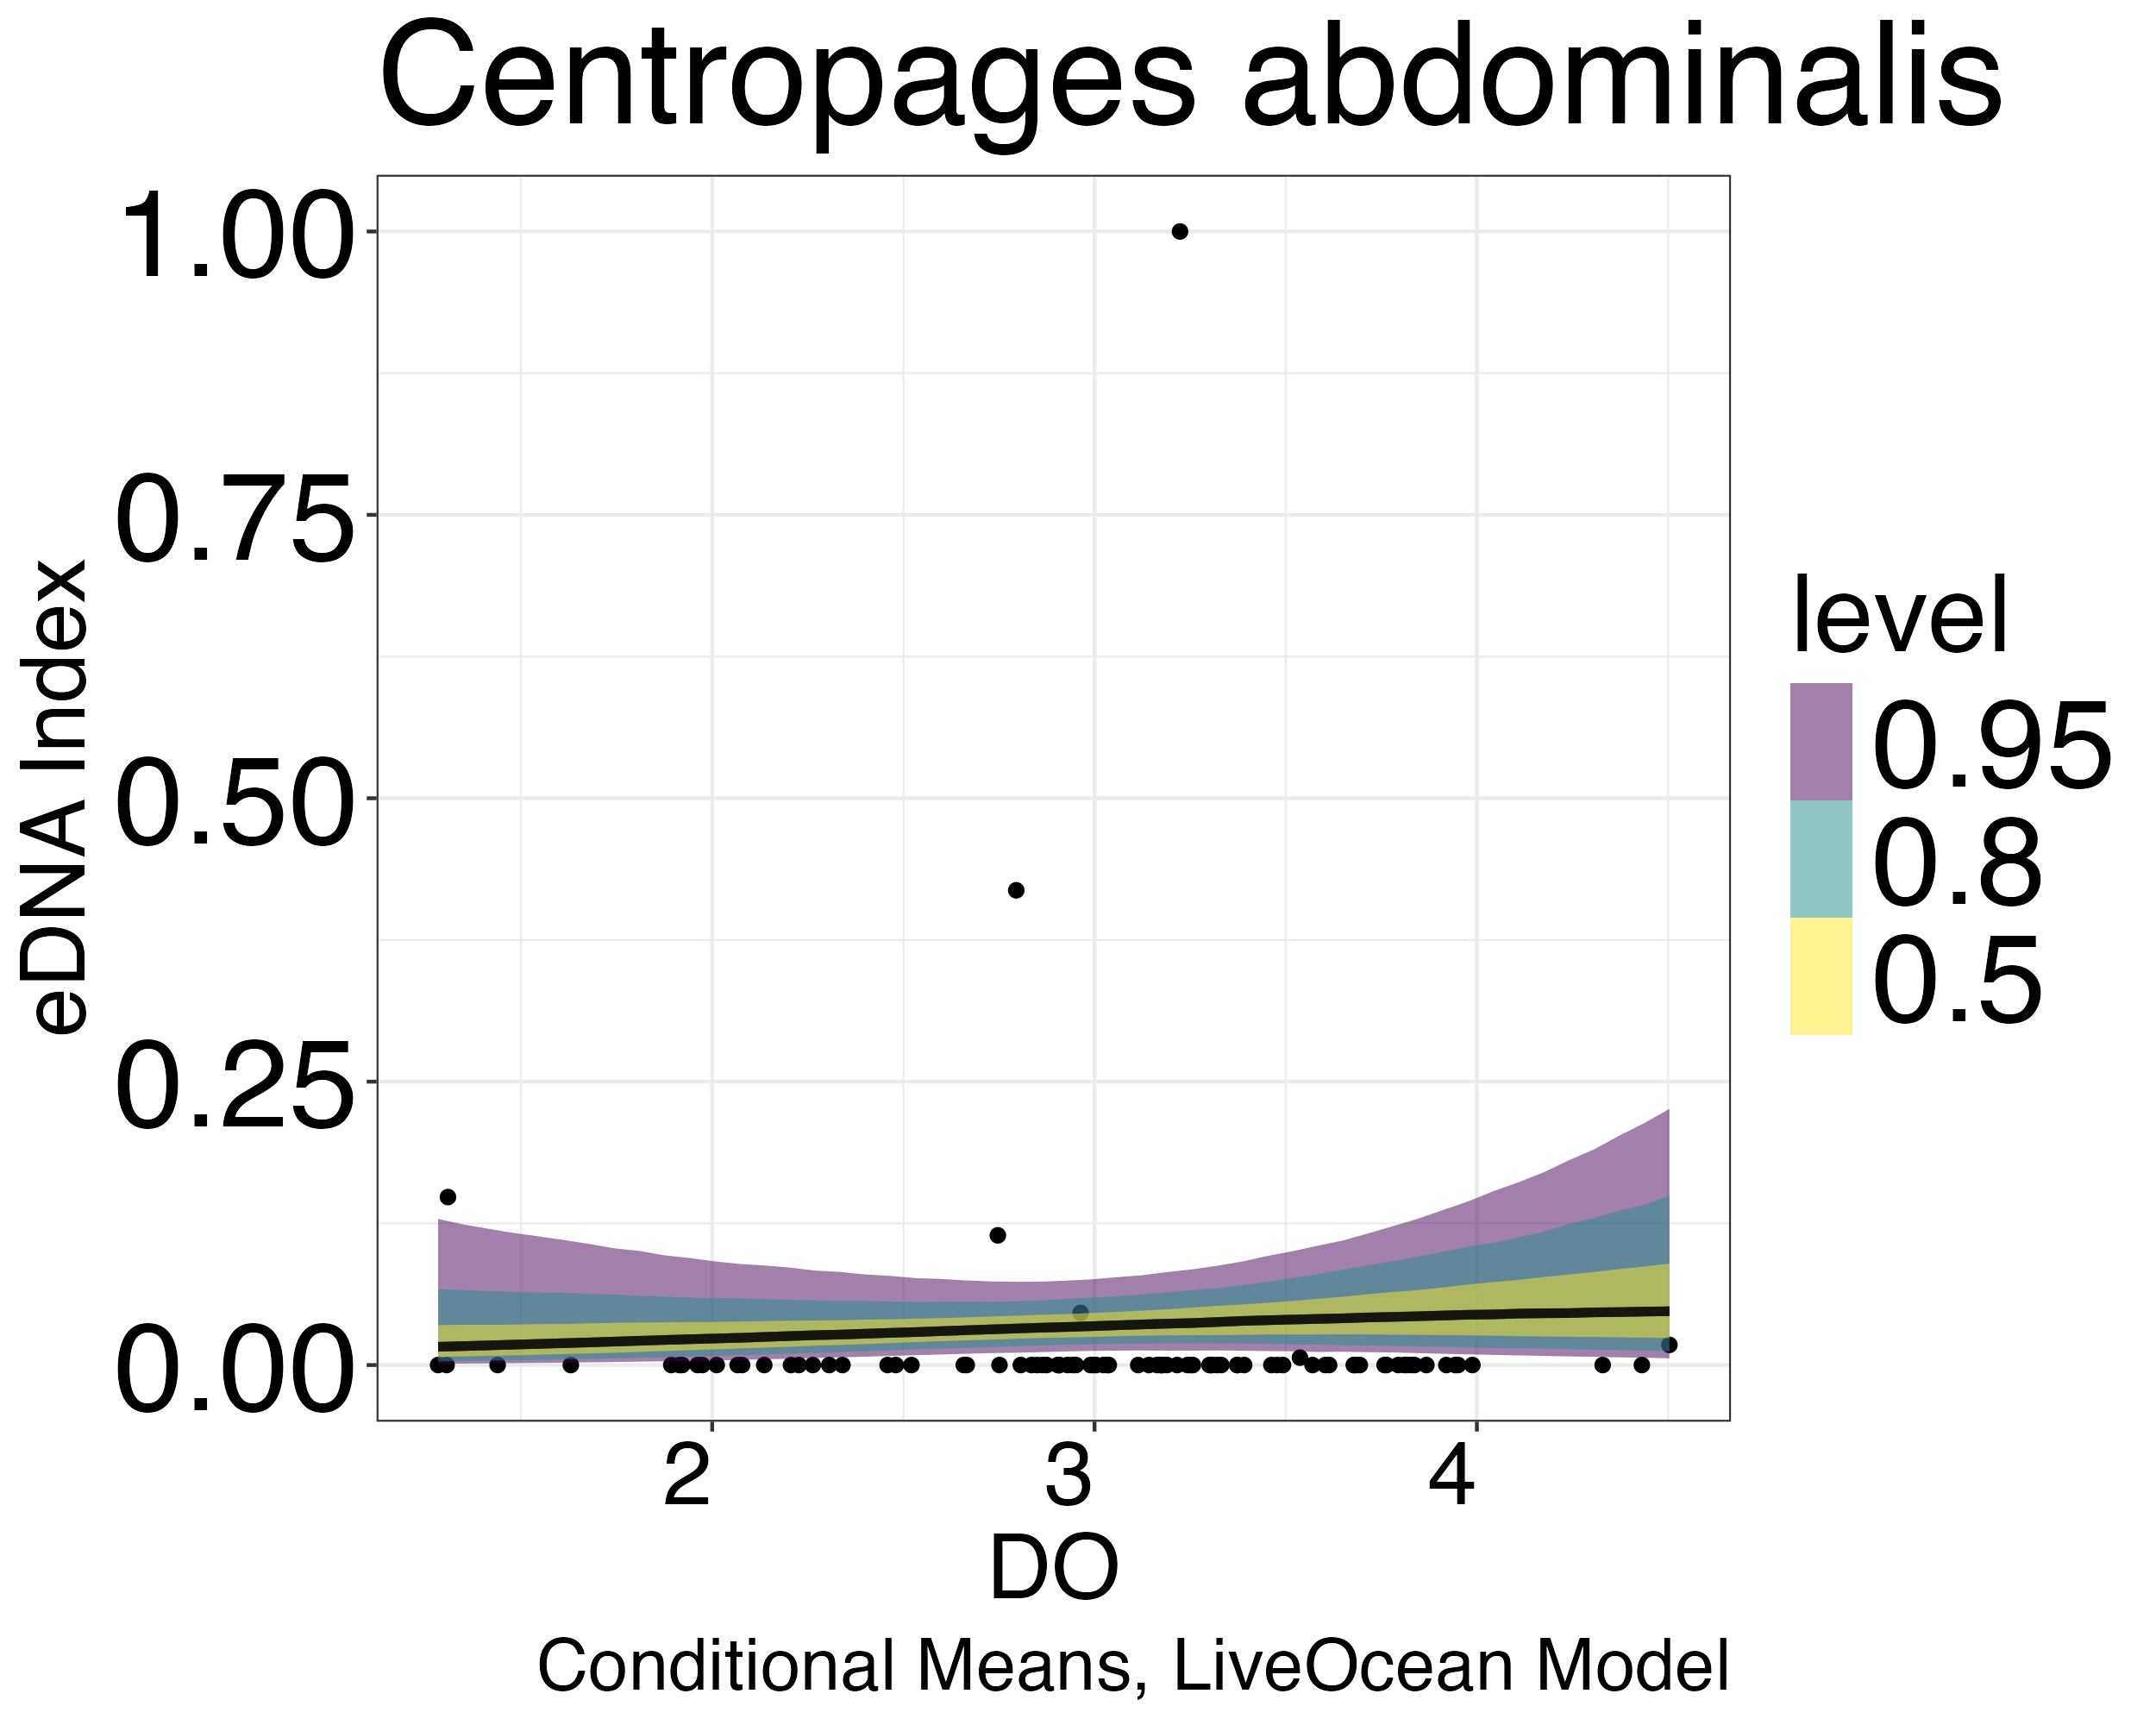
\includegraphics[scale=0.25]{Cabdominalis_ZOIB_Means_Mod_noOut}
			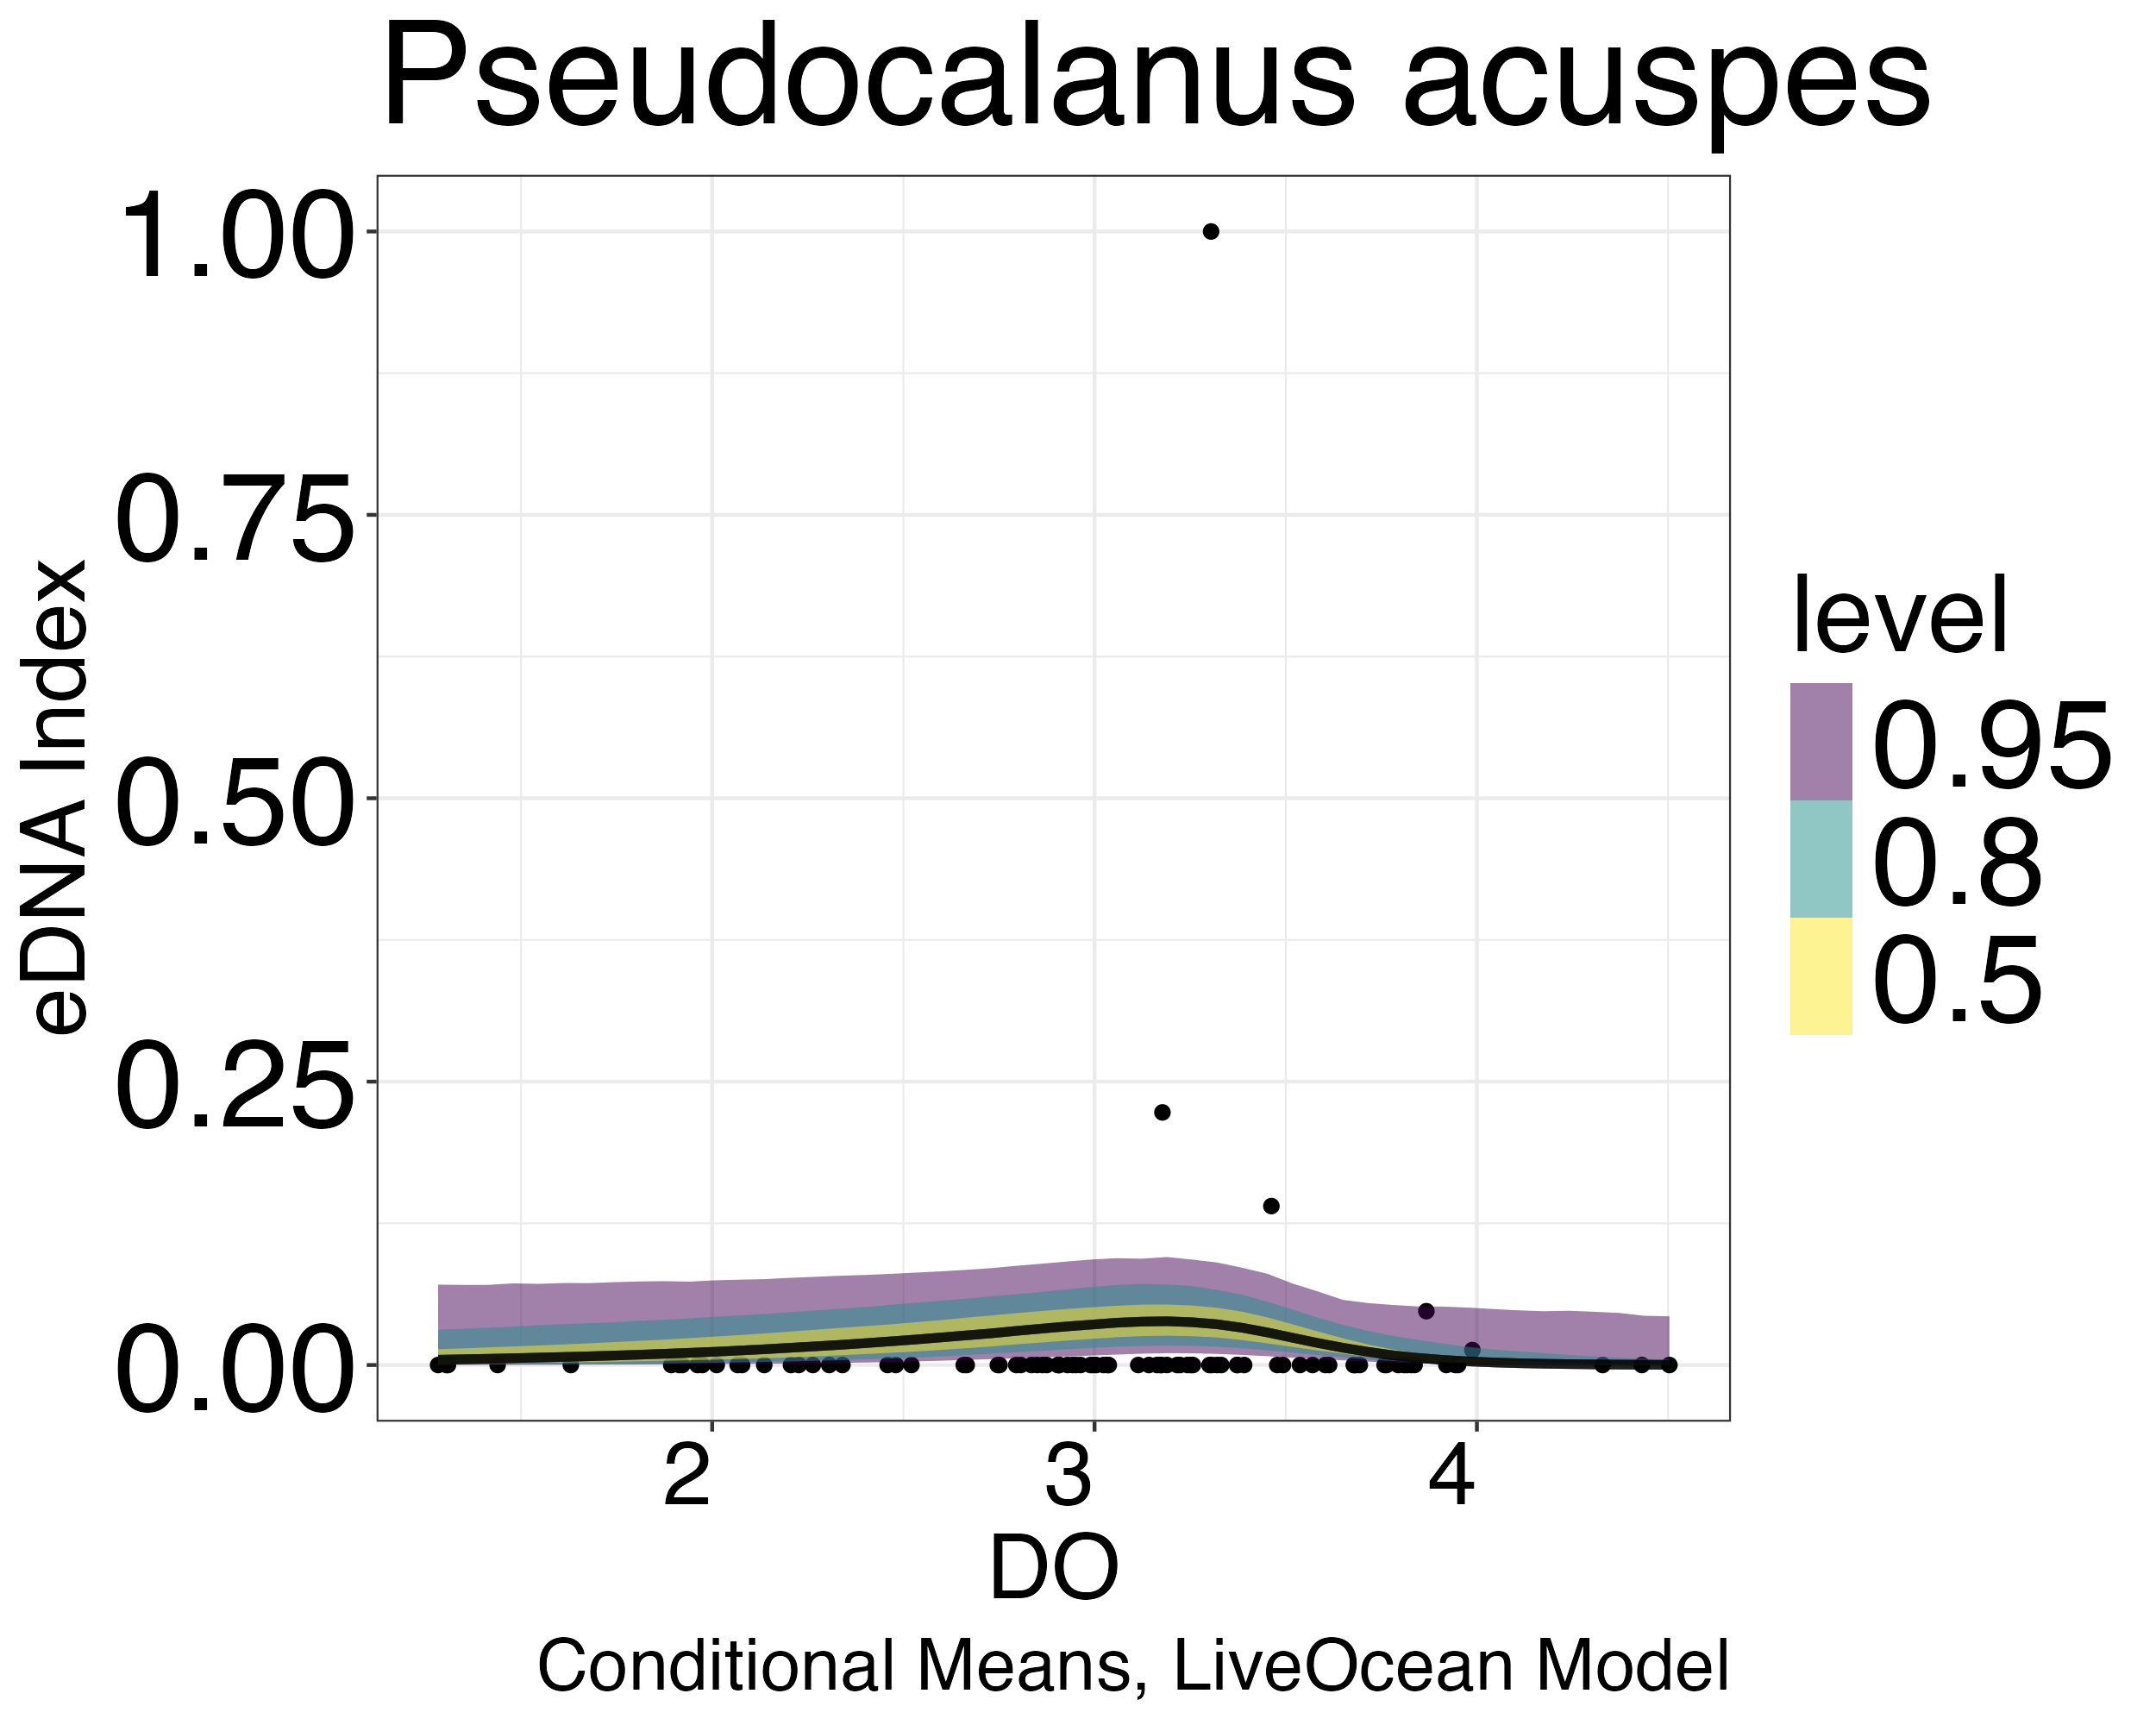
\includegraphics[scale=0.25]{Pacuspes_ZOIB_Means_Mod_noOut} \\
			Year-round: \\
			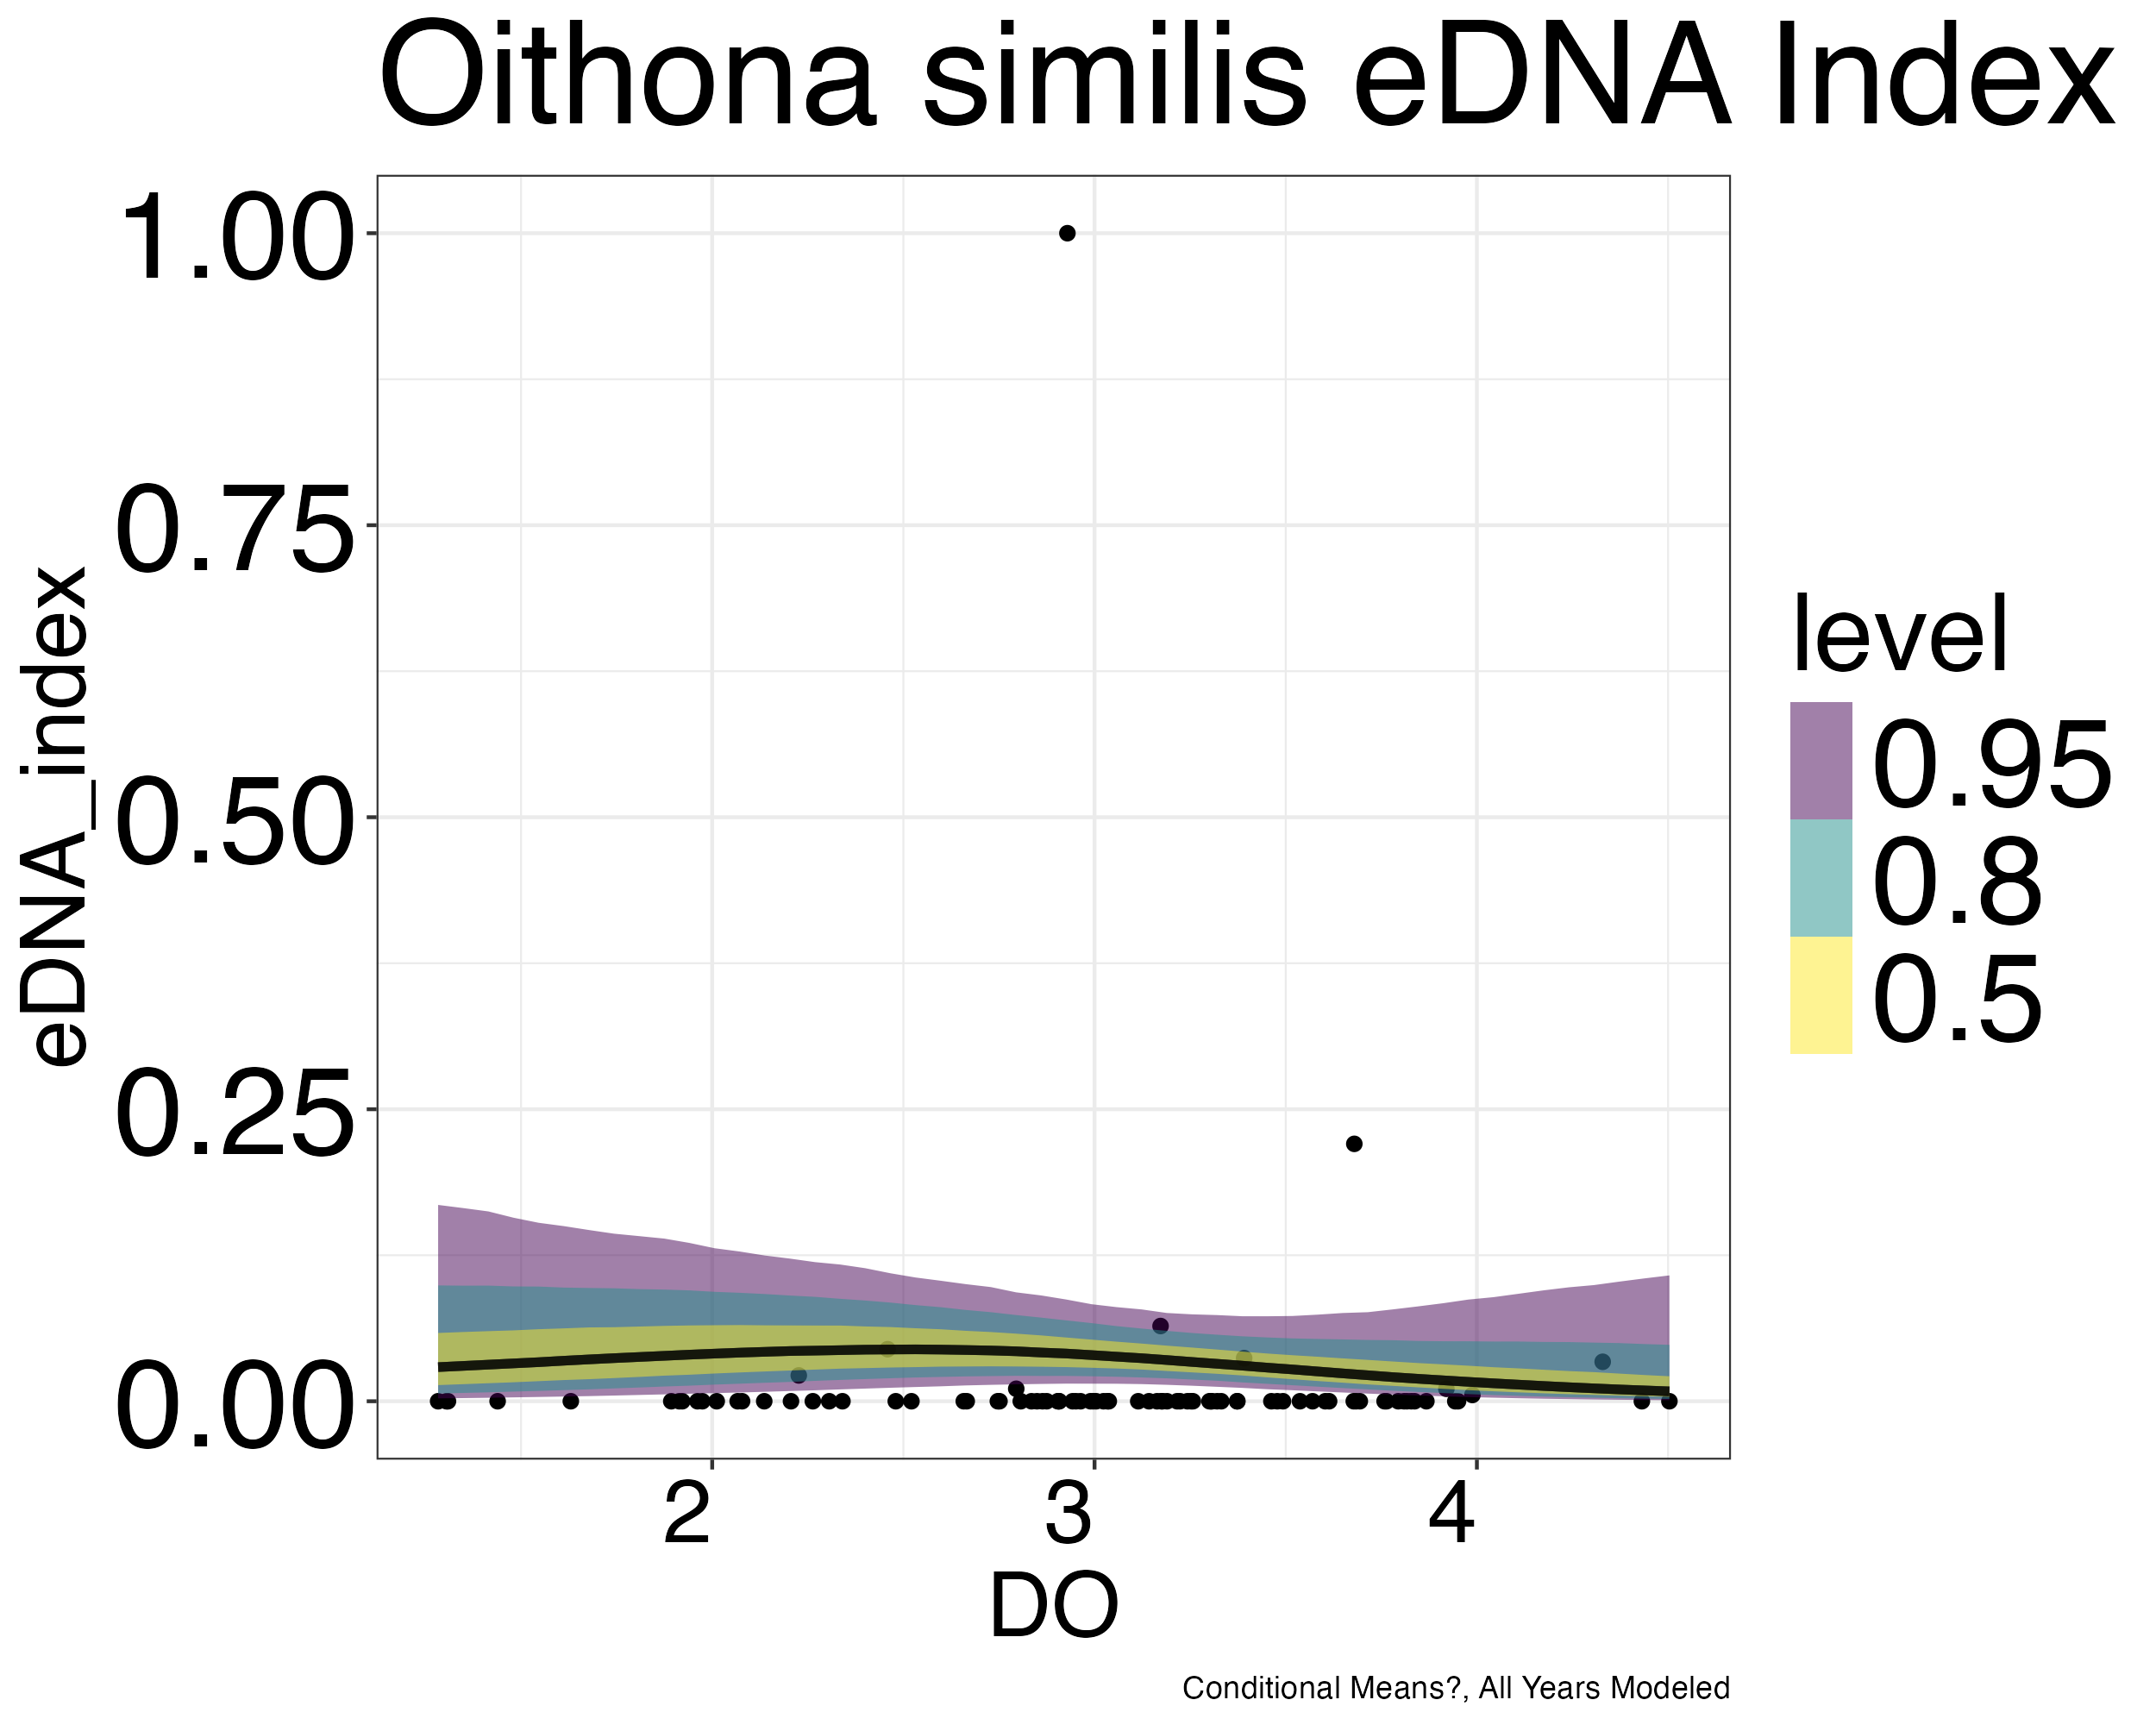
\includegraphics[scale=0.25]{Osimilis_ZOIB_Means_Mod_noOut} \\
			Southern: \\
			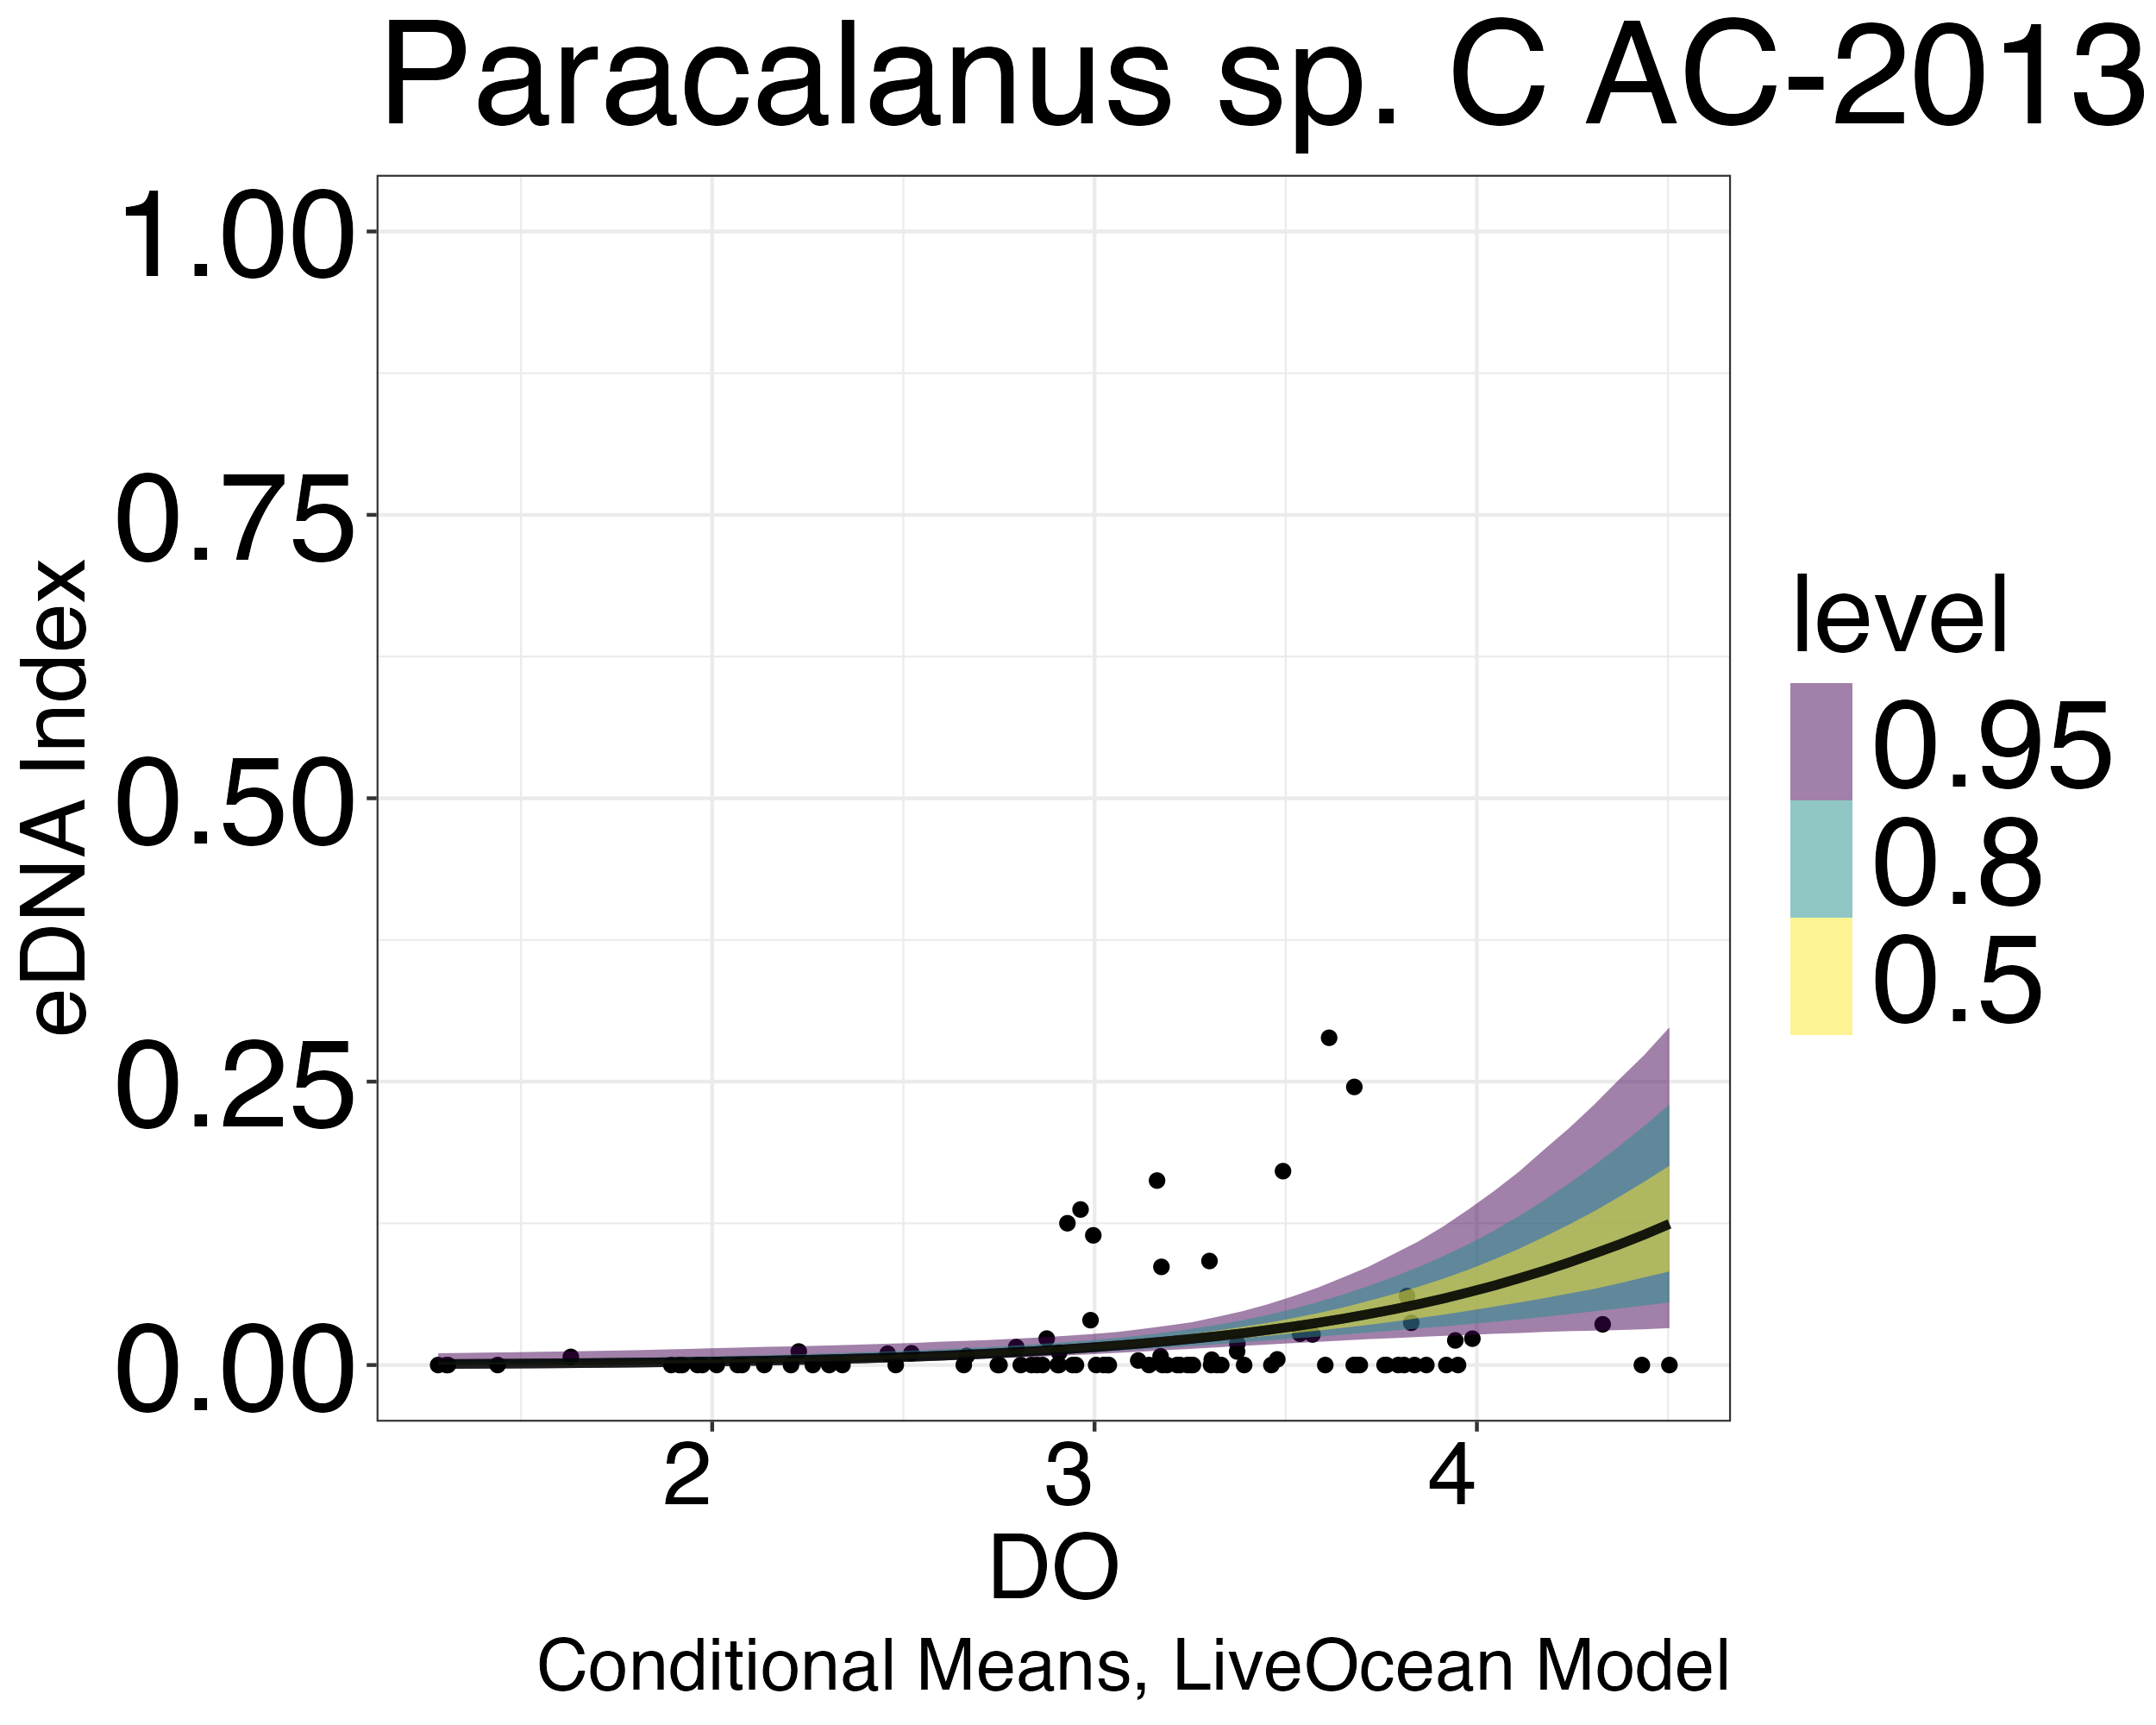
\includegraphics[scale=0.25]{Paracalanus_ZOIB_Means_Mod_noOut}
			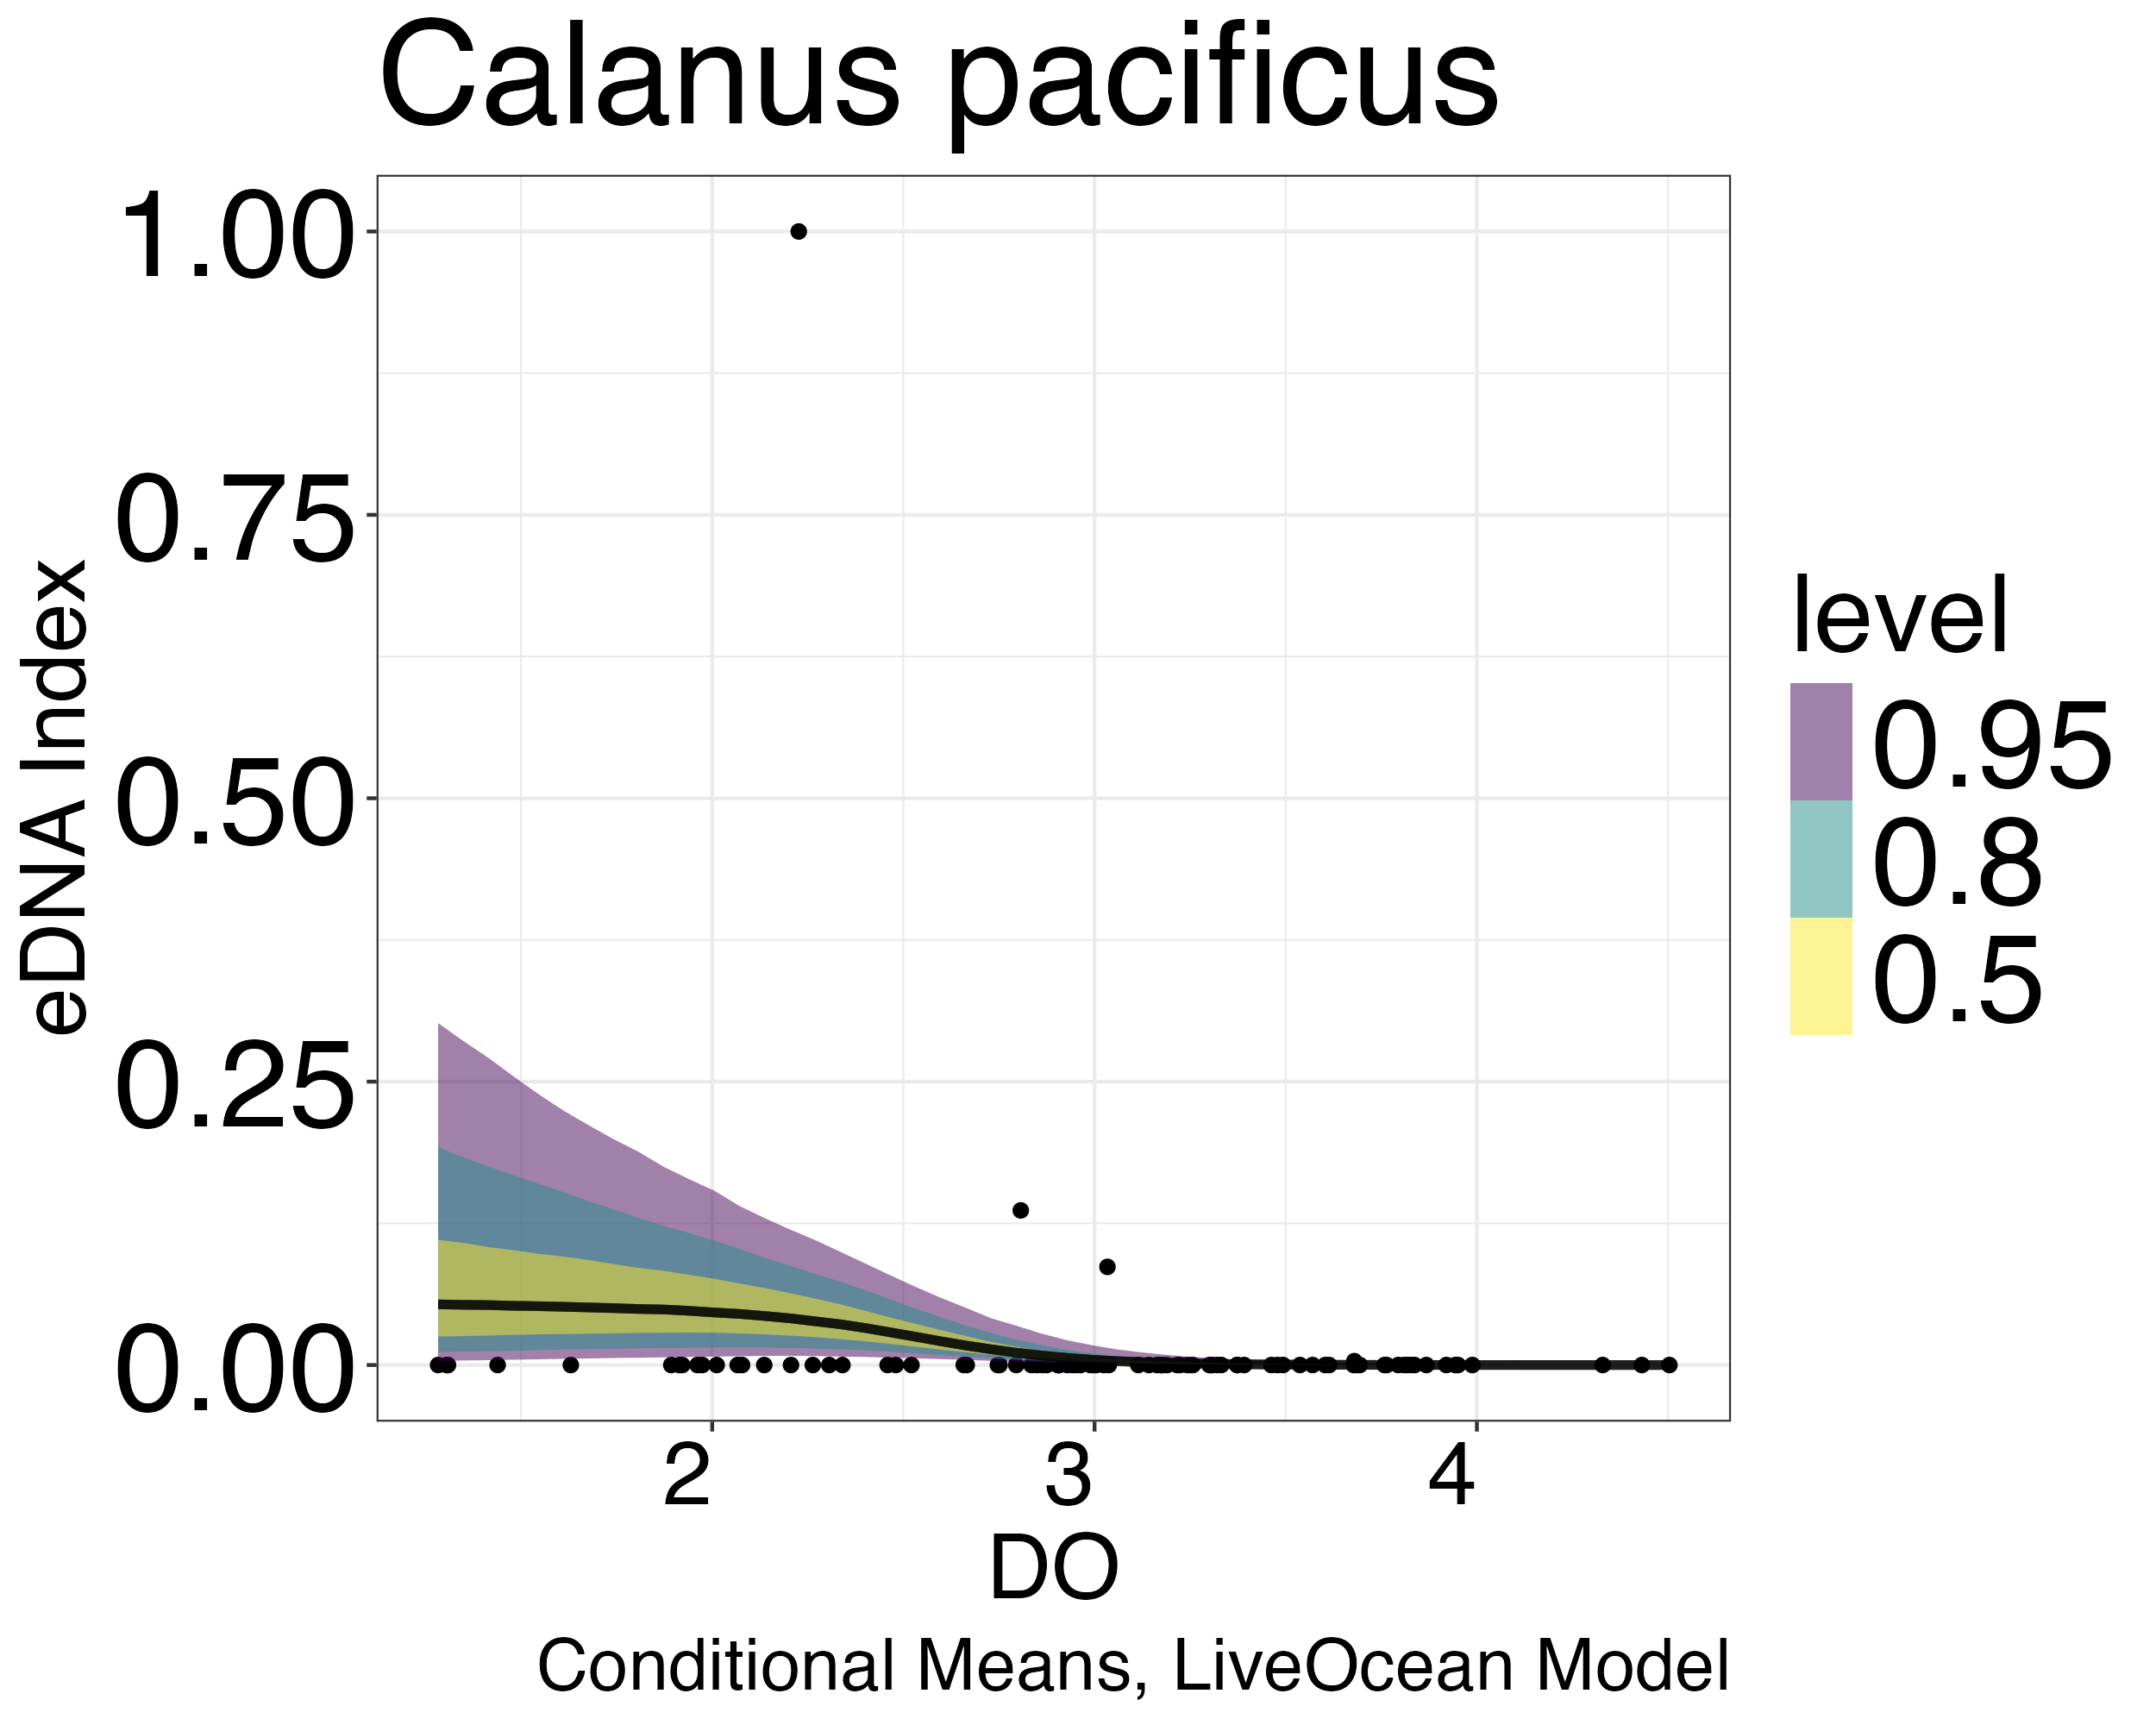
\includegraphics[scale=0.25]{Cpacificus_ZOIB_Means_Mod_noOut}
			\caption[Zero-inflated beta regression means (modeled data)]{\footnotesize{Zero-inflated beta regression model means, with bands showing 0.5, 0.8, and 0.95 confidence levels, using data from 2021-23 from the LiveOcean model.}} %the special ToC caption is in square brackets. The \footnotesize makes the figure caption smaller
			\label{ModZOIB}
		\end{center}
	\end{figure}
	
	\chapter{Additional Plots of Dissolved Oxygen vs. Temperature vs. eDNA Index}\label{chap:appPlots}
	%Other
	
	\begin{figure}[!h]
		\begin{center}
			a. 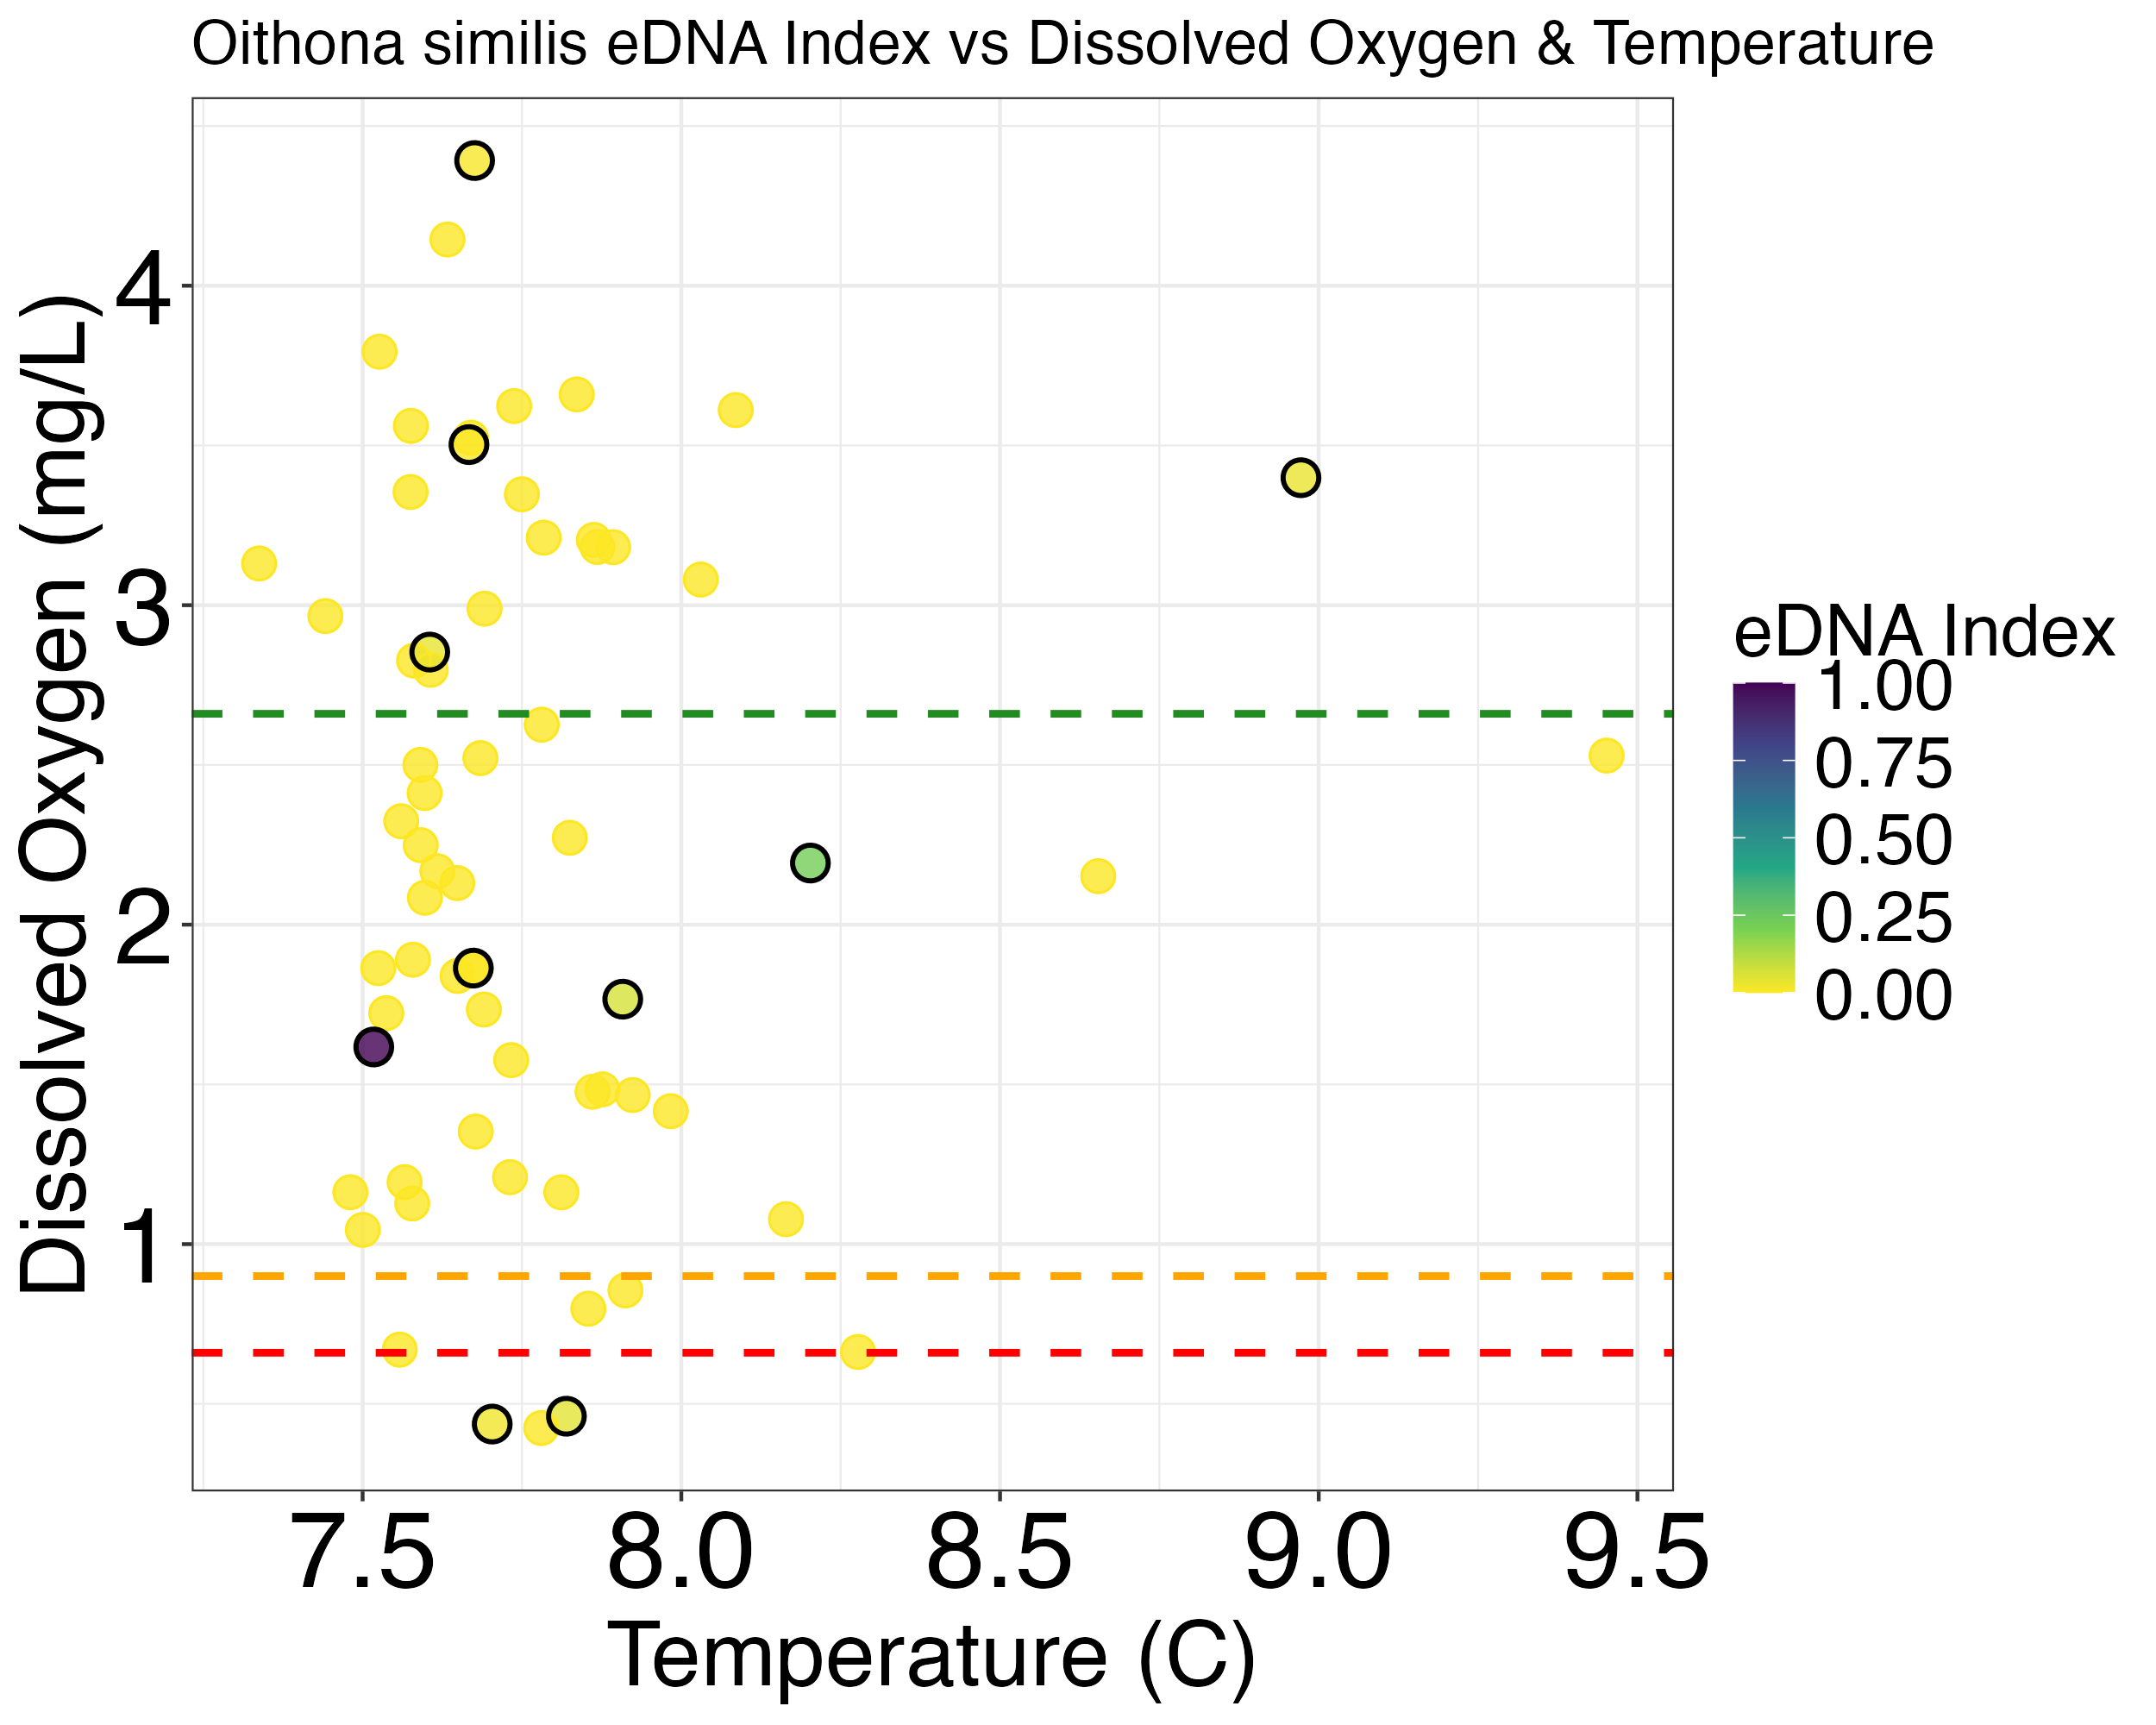
\includegraphics[scale=0.3]{Osimilis_Scatter_noOut}
			b. 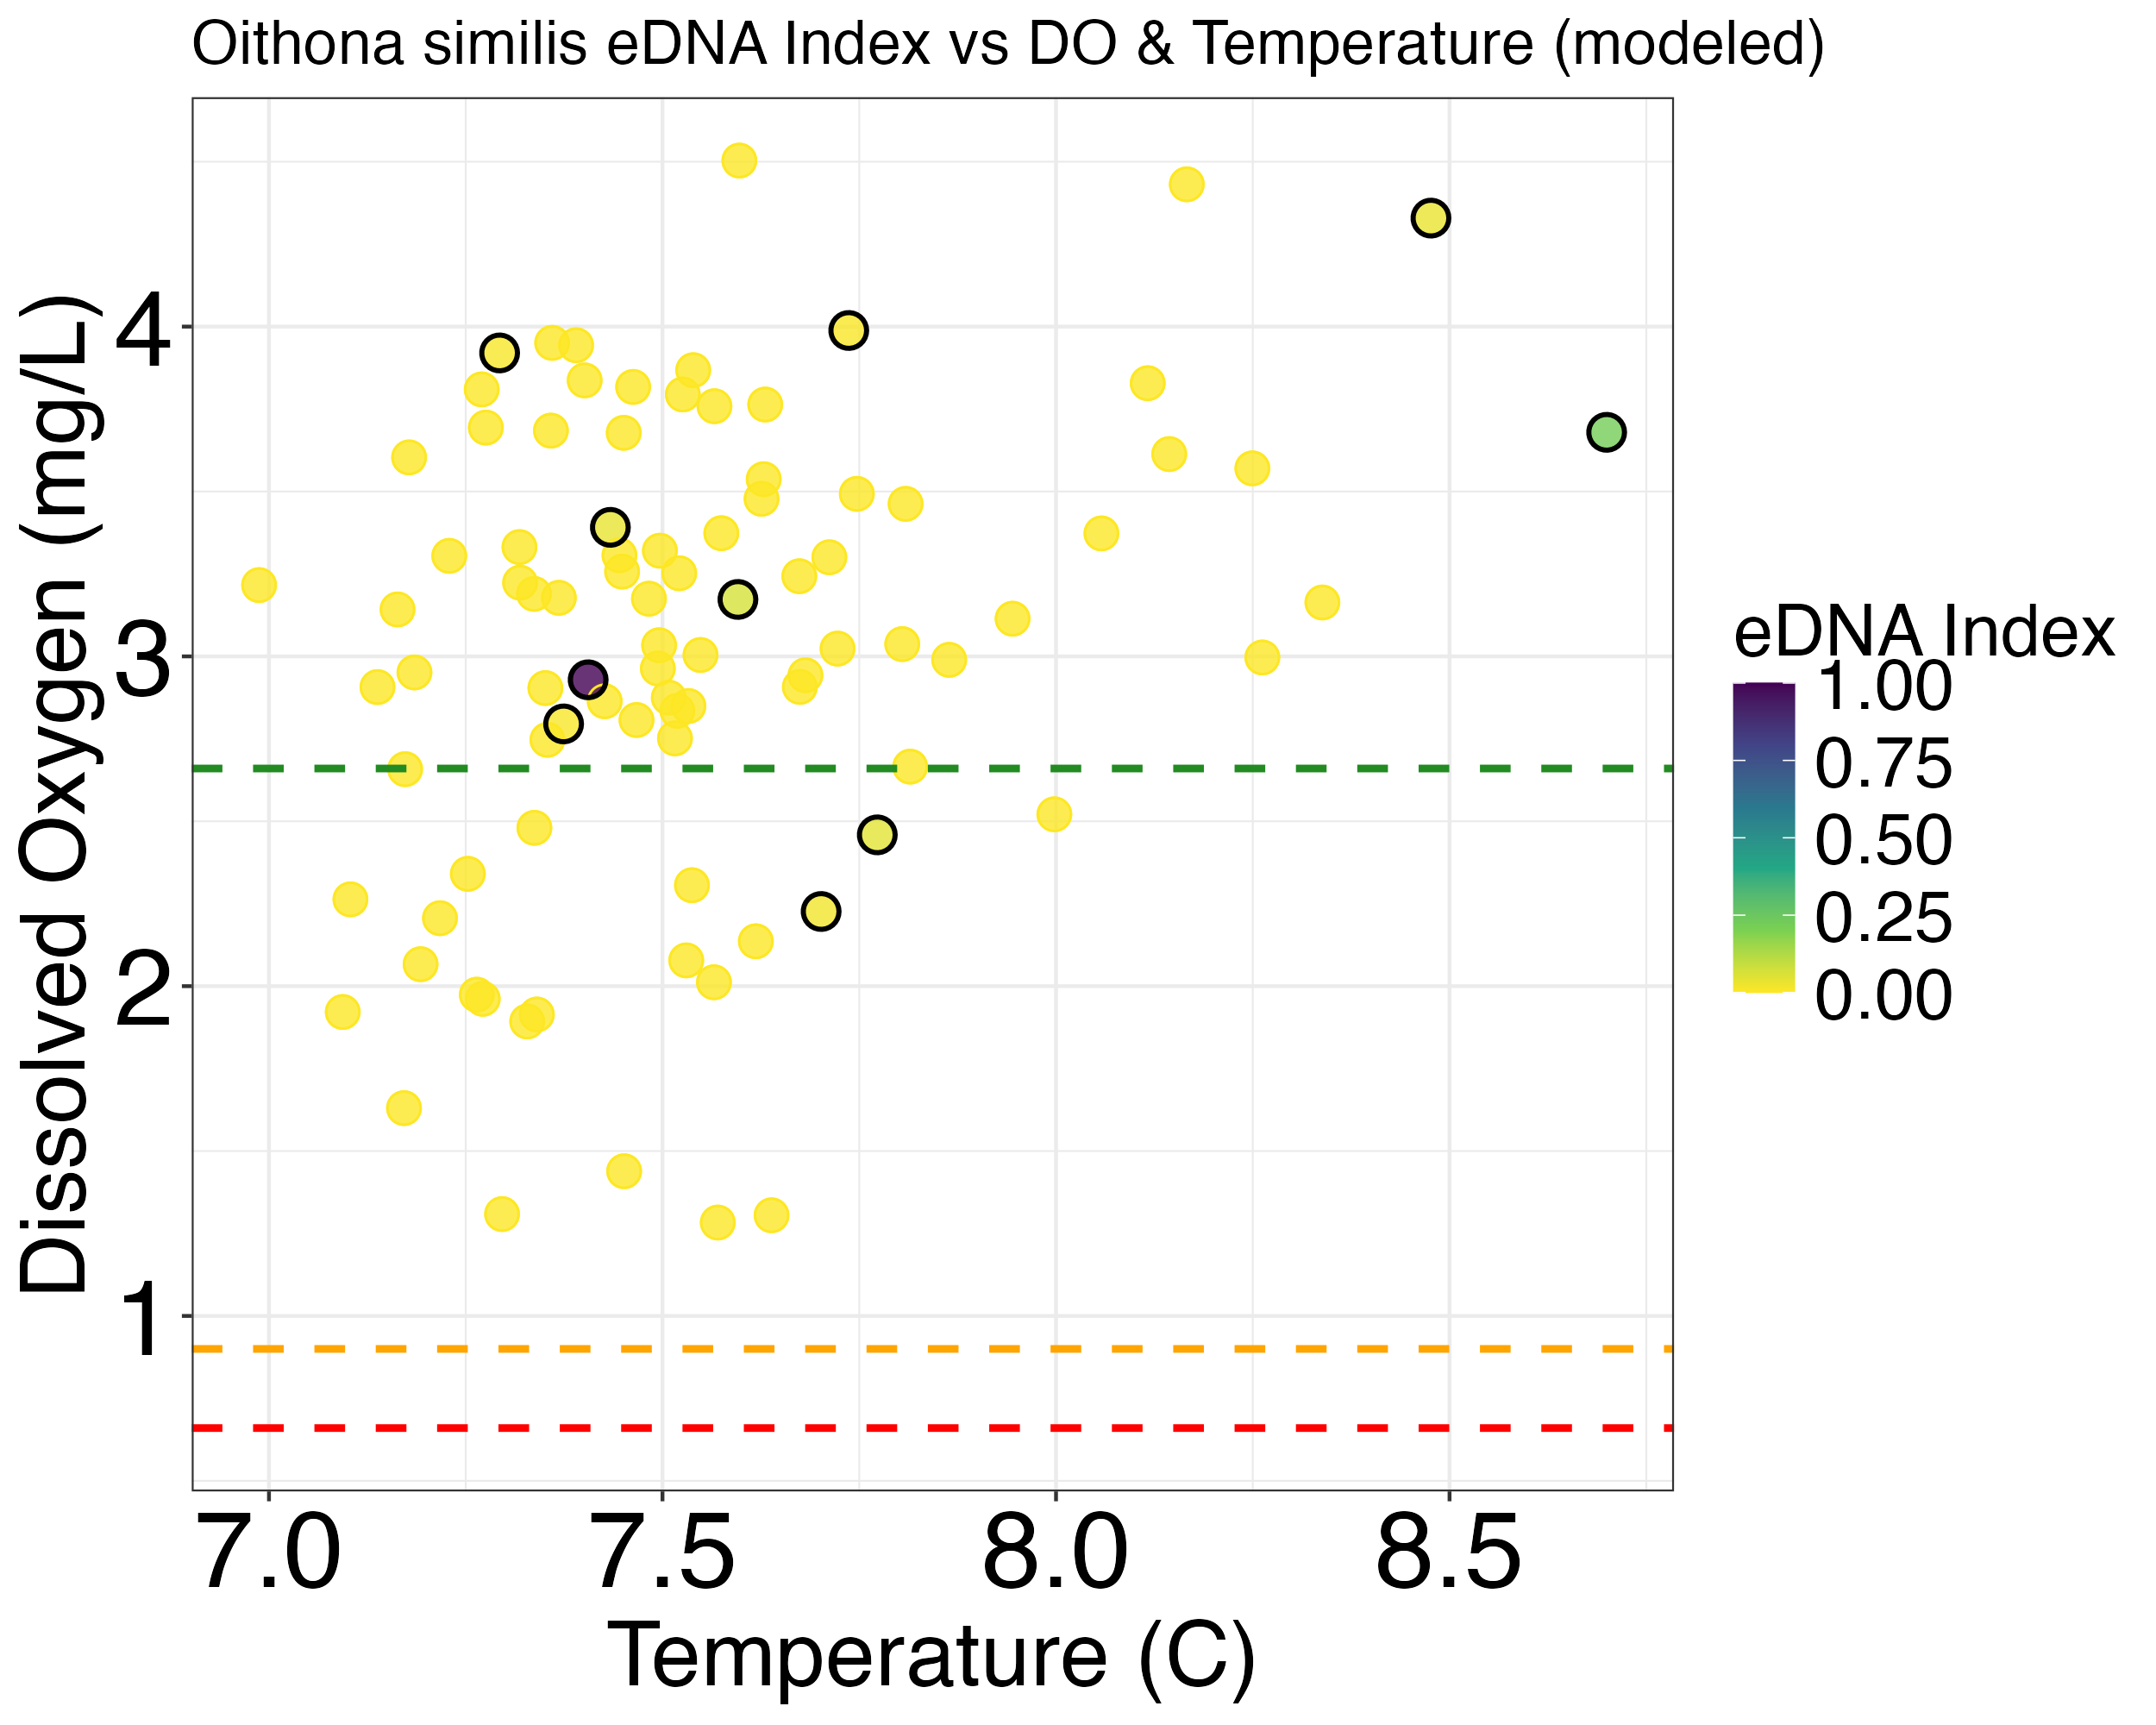
\includegraphics[scale=0.3]{Osimilis_Scatter_AllYr_mod_noOut}
			\caption[\textit{O. similis} scatterplot]{\footnotesize{Scatterplot of dissolved oxygen (mg/L) and temperature (Celsius) for each environmental DNA sampling time, with \textit{O. similis} detections circled in black. Color of dots represents eDNA index, a normalized measure of abundance that can compare abundance within a species. Yellow, uncircled dots represent sampling dates when \textit{O. similis} was not detected. Plot (a) uses TH042 mooring data from 2021-22, (b) uses LiveOcean model data from 2021-23.}} %the special ToC caption is in square brackets. The \footnotesize makes the figure caption smaller
			\label{OsimilisScatter}
		\end{center}
	\end{figure} 
	
	%Northern
	\begin{figure}[!h]
		\begin{center}
			a. 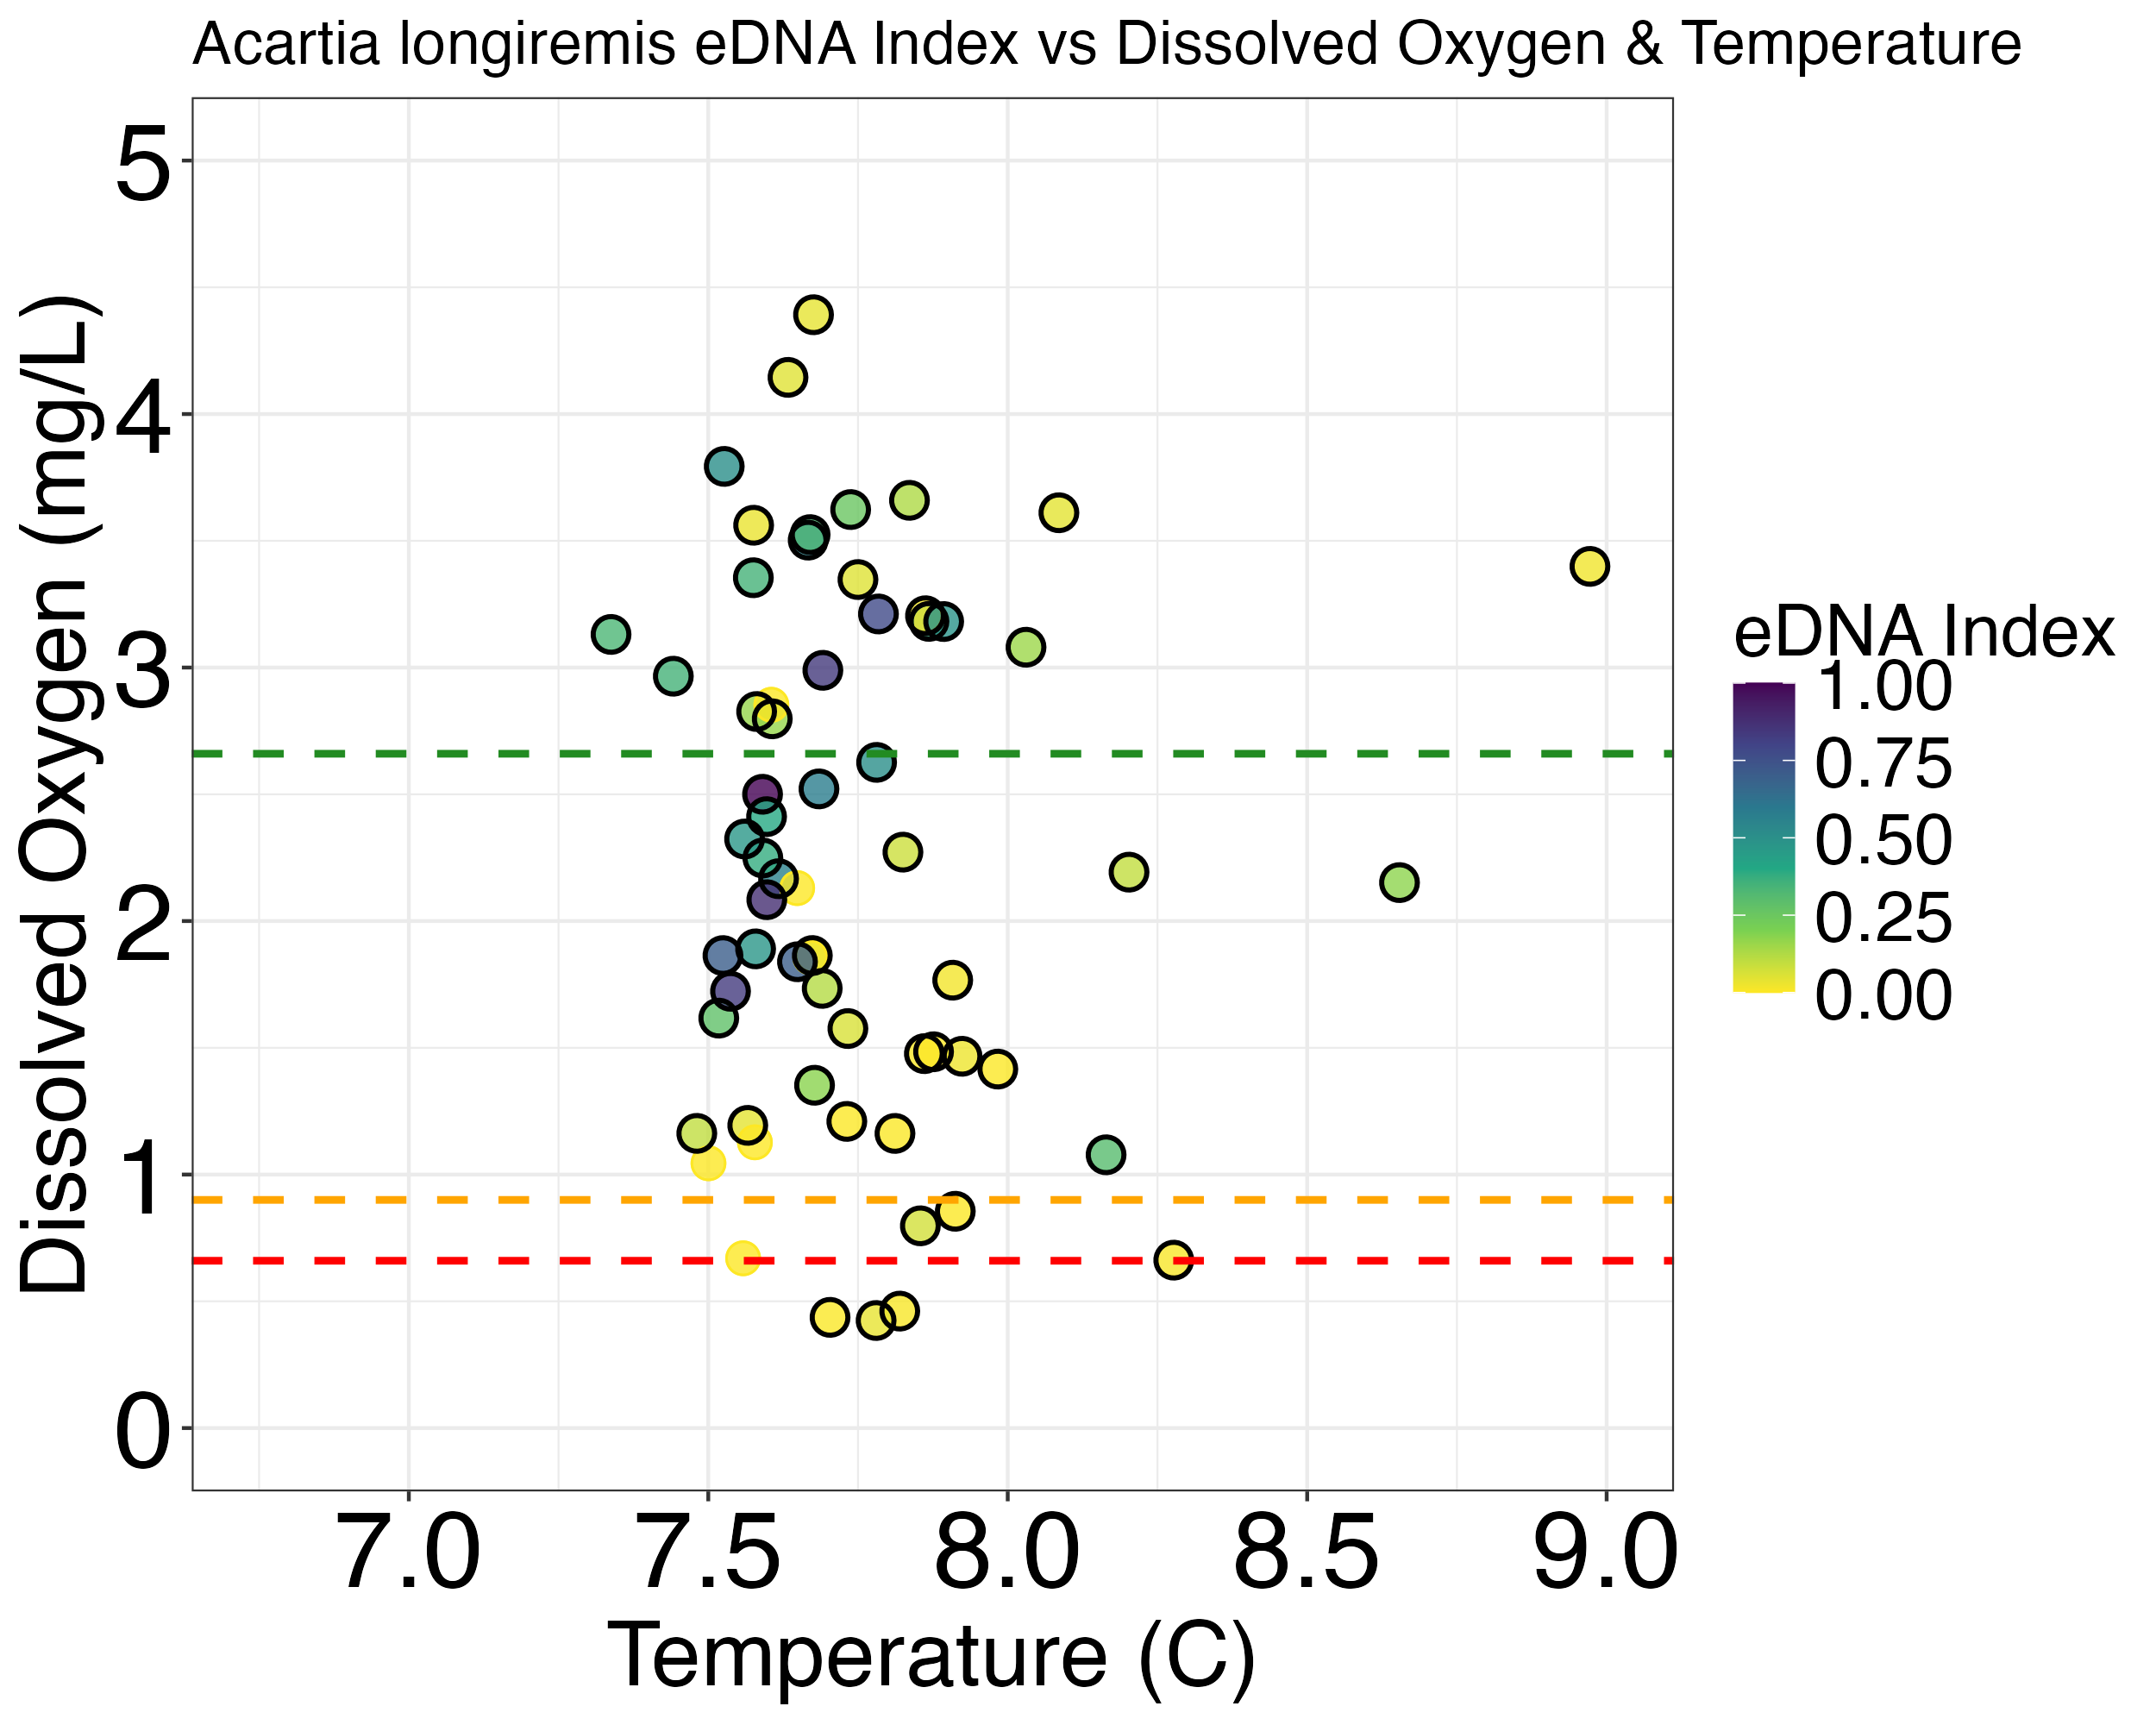
\includegraphics[scale=0.3]{Alongiremis_Scatter_noOut}
			b. 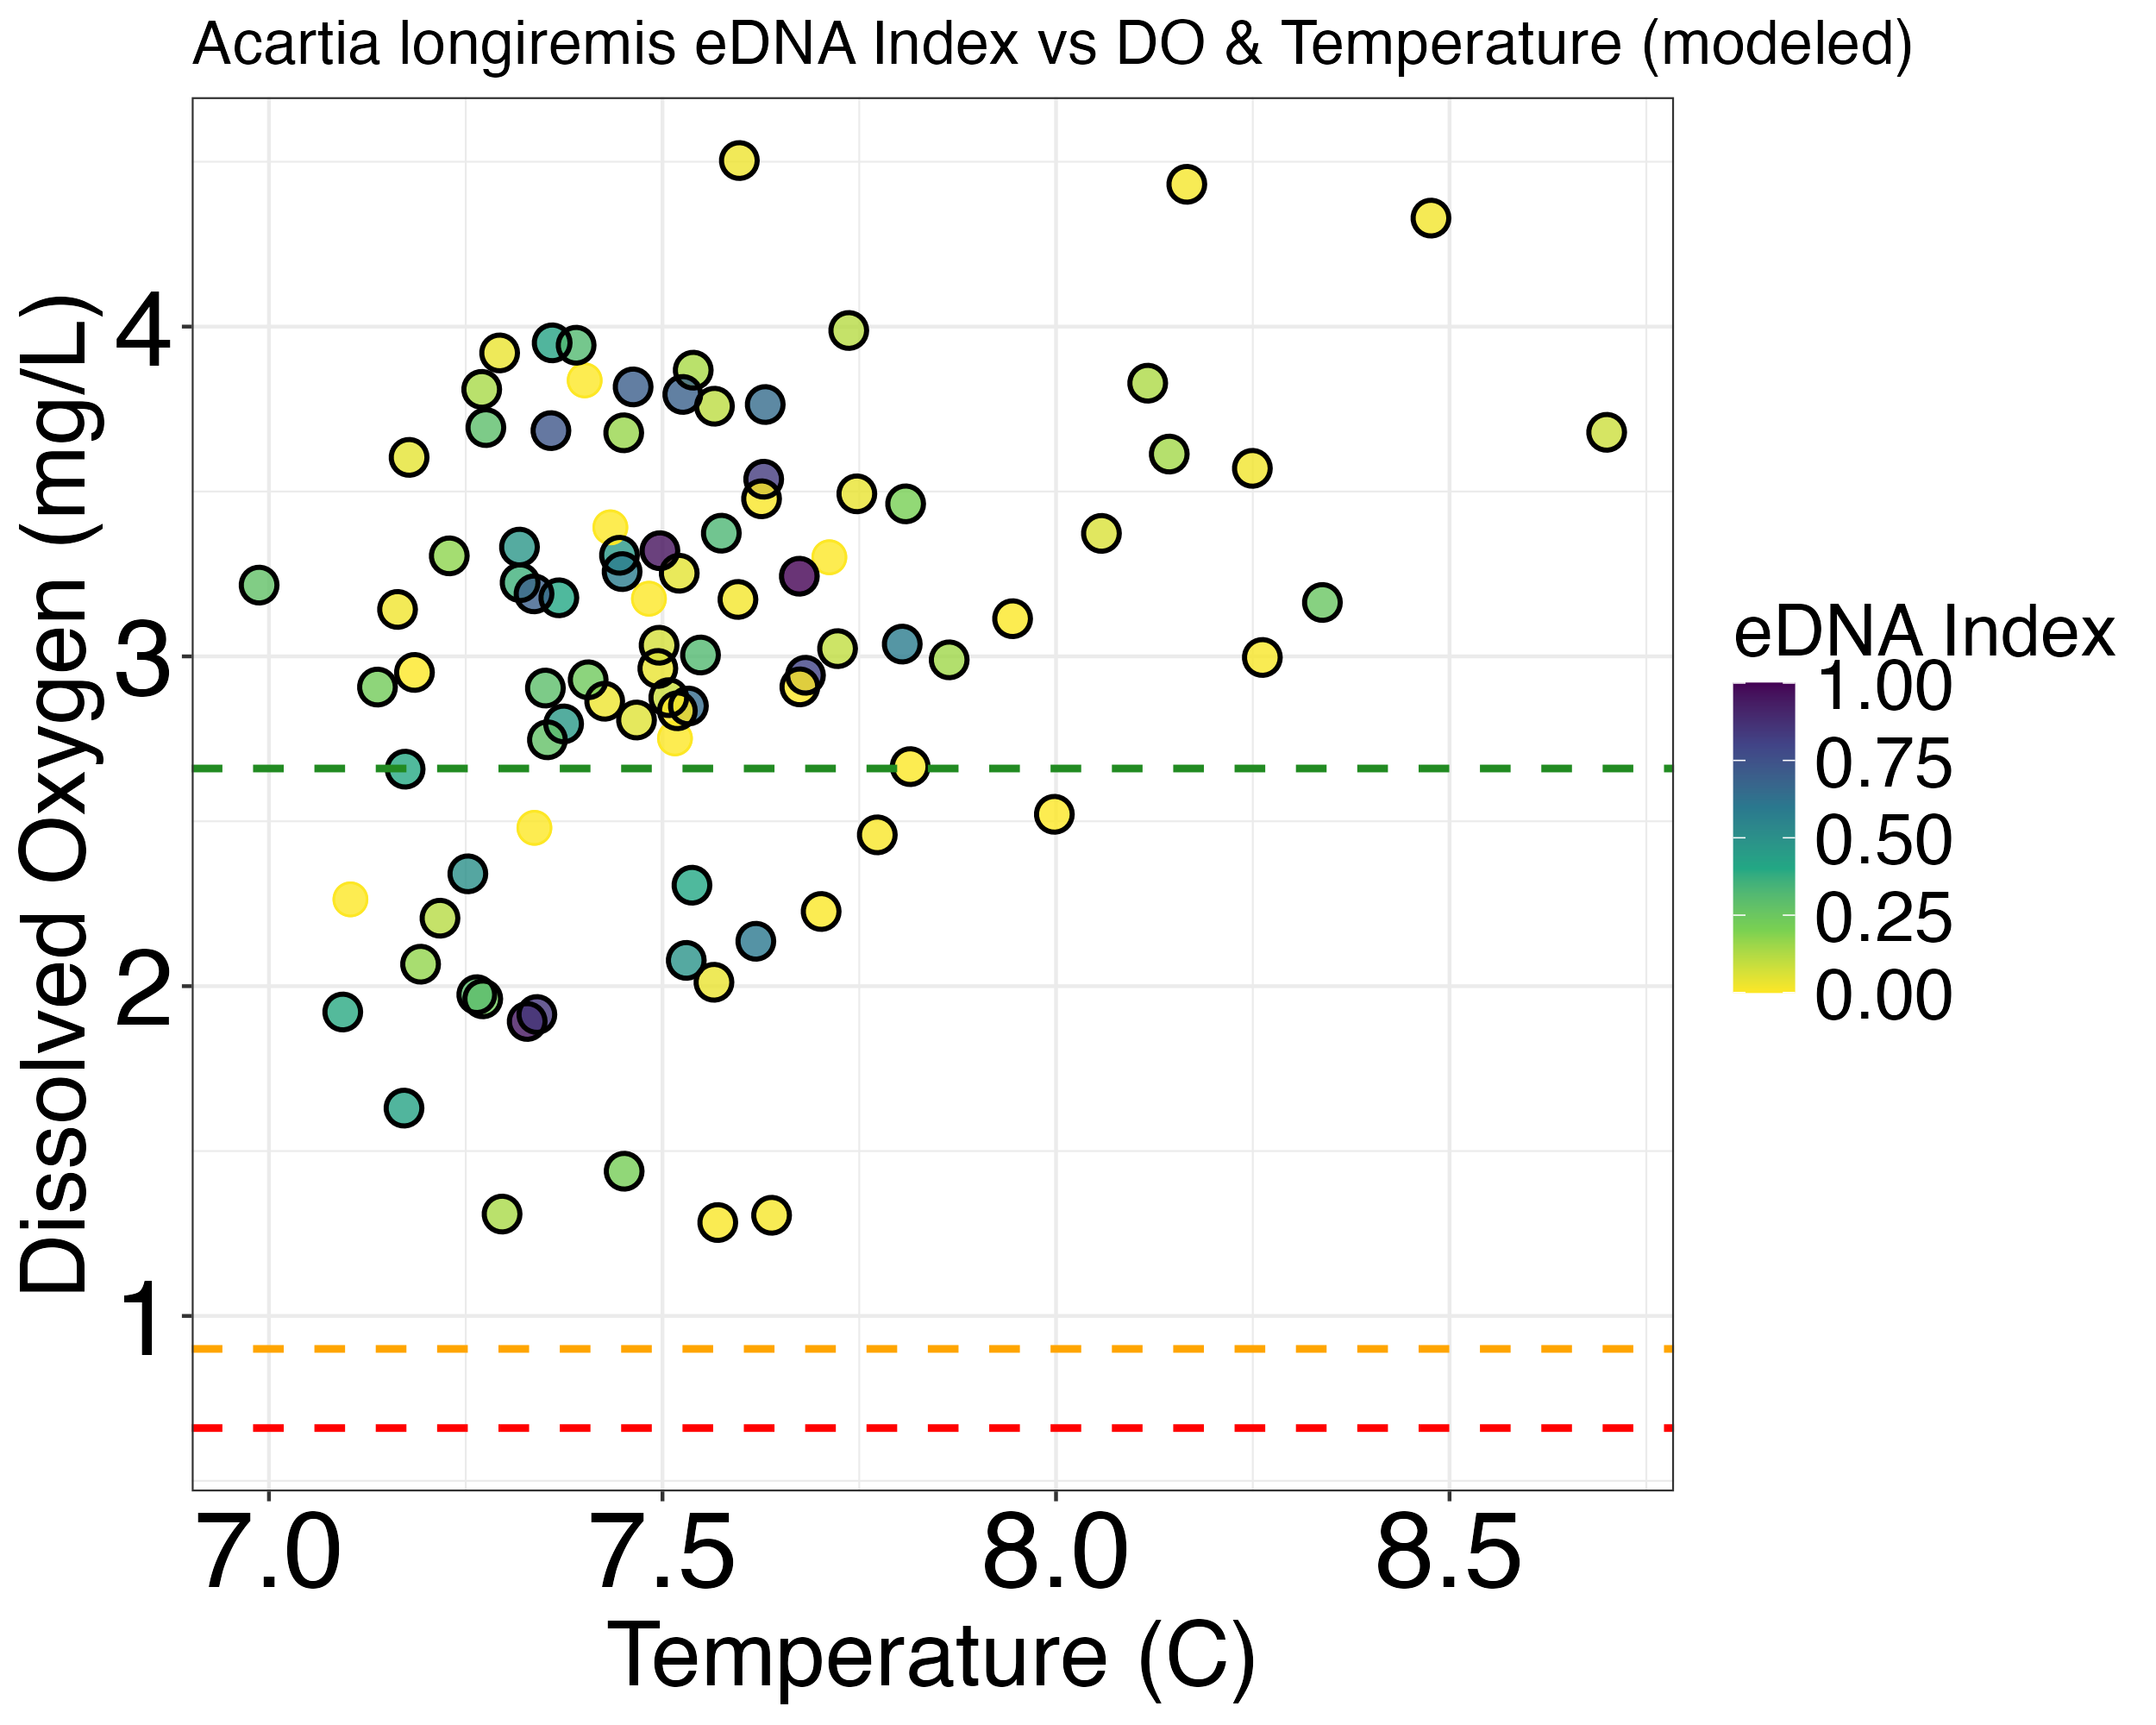
\includegraphics[scale=0.3]{Alongiremis_Scatter_AllYr_mod_noOut}
			\caption[\textit{A. longiremis} scatterplot]{\footnotesize{Scatterplot of dissolved oxygen (mg/L) and temperature (Celsius) for each environmental DNA sampling time, with \textit{A. longiremis} detections circled in black. Color of dots represents eDNA index, a normalized measure of abundance that can compare abundance within a species. Yellow, uncircled dots represent sampling dates when \textit{A. longiremis} was not detected. Plot (a) uses TH042 mooring data from 2021-22, (b) uses LiveOcean model data from 2021-23.}} %the special ToC caption is in square brackets. The \footnotesize makes the figure caption smaller
			\label{AlongiremisScatter}
		\end{center}
	\end{figure} 
	
	\begin{figure}[!h]
		\begin{center}
			a. 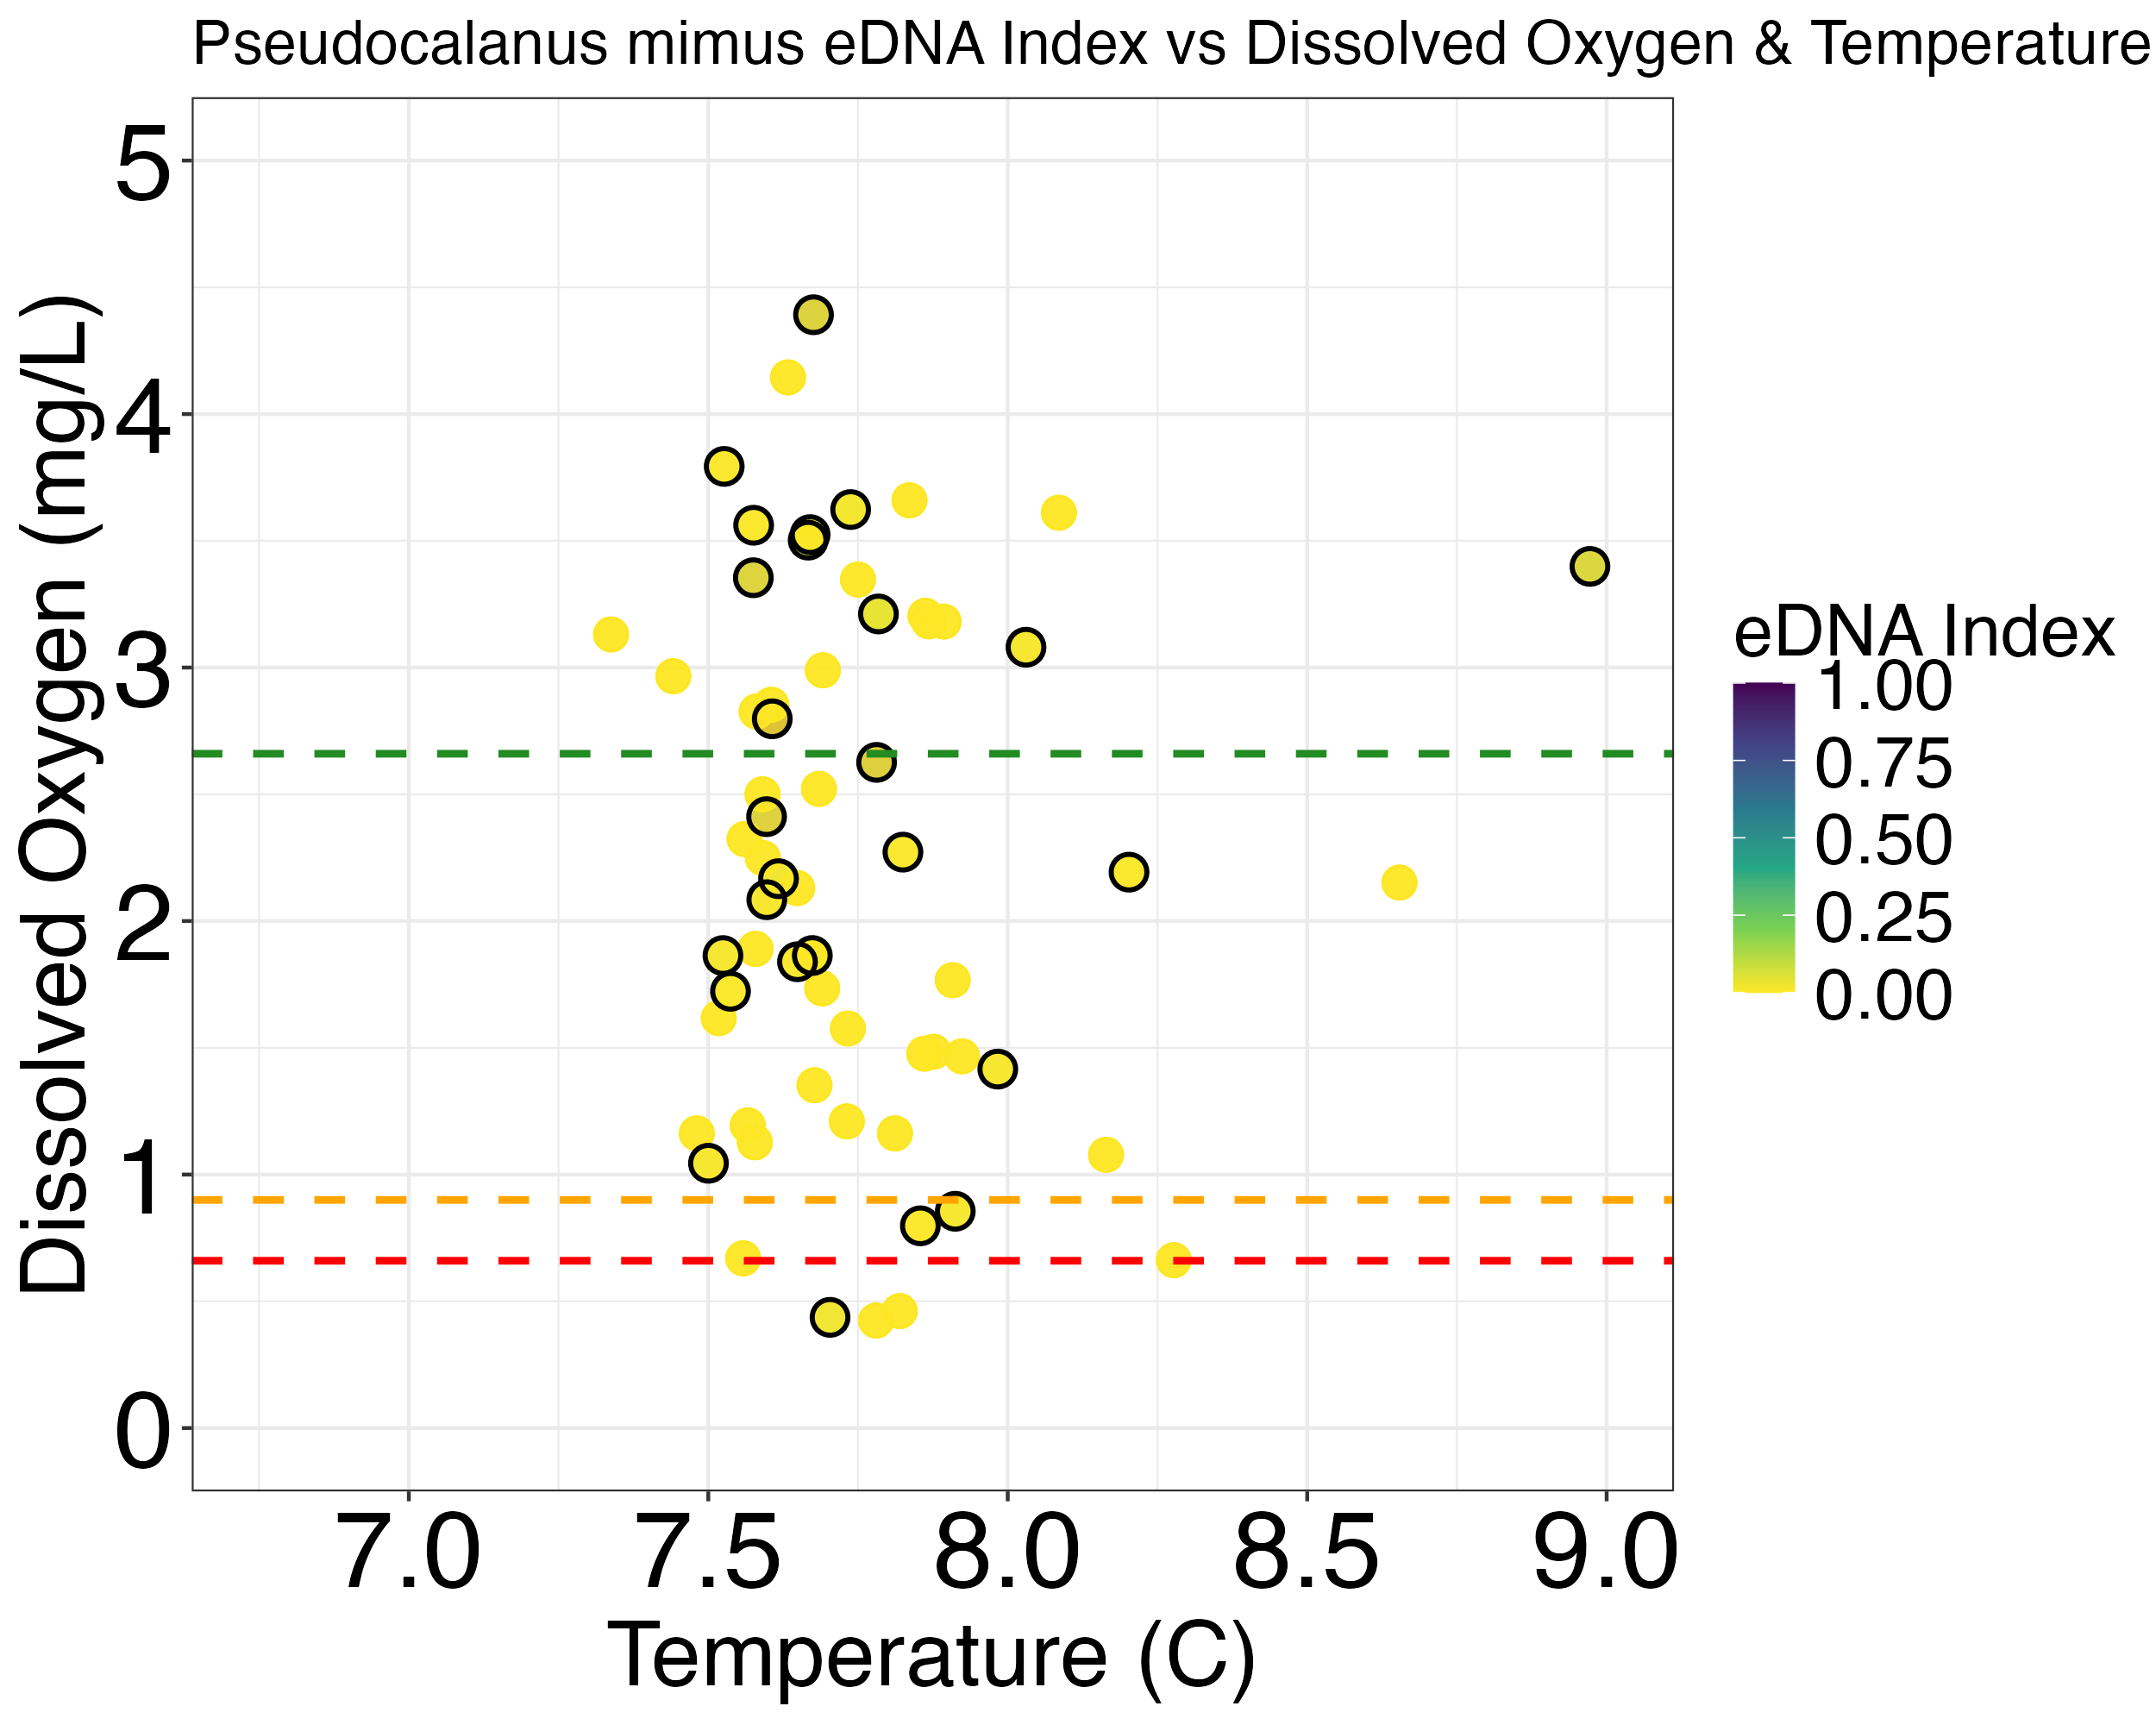
\includegraphics[scale=0.3]{Pmimus_Scatter_noOut}
			b. 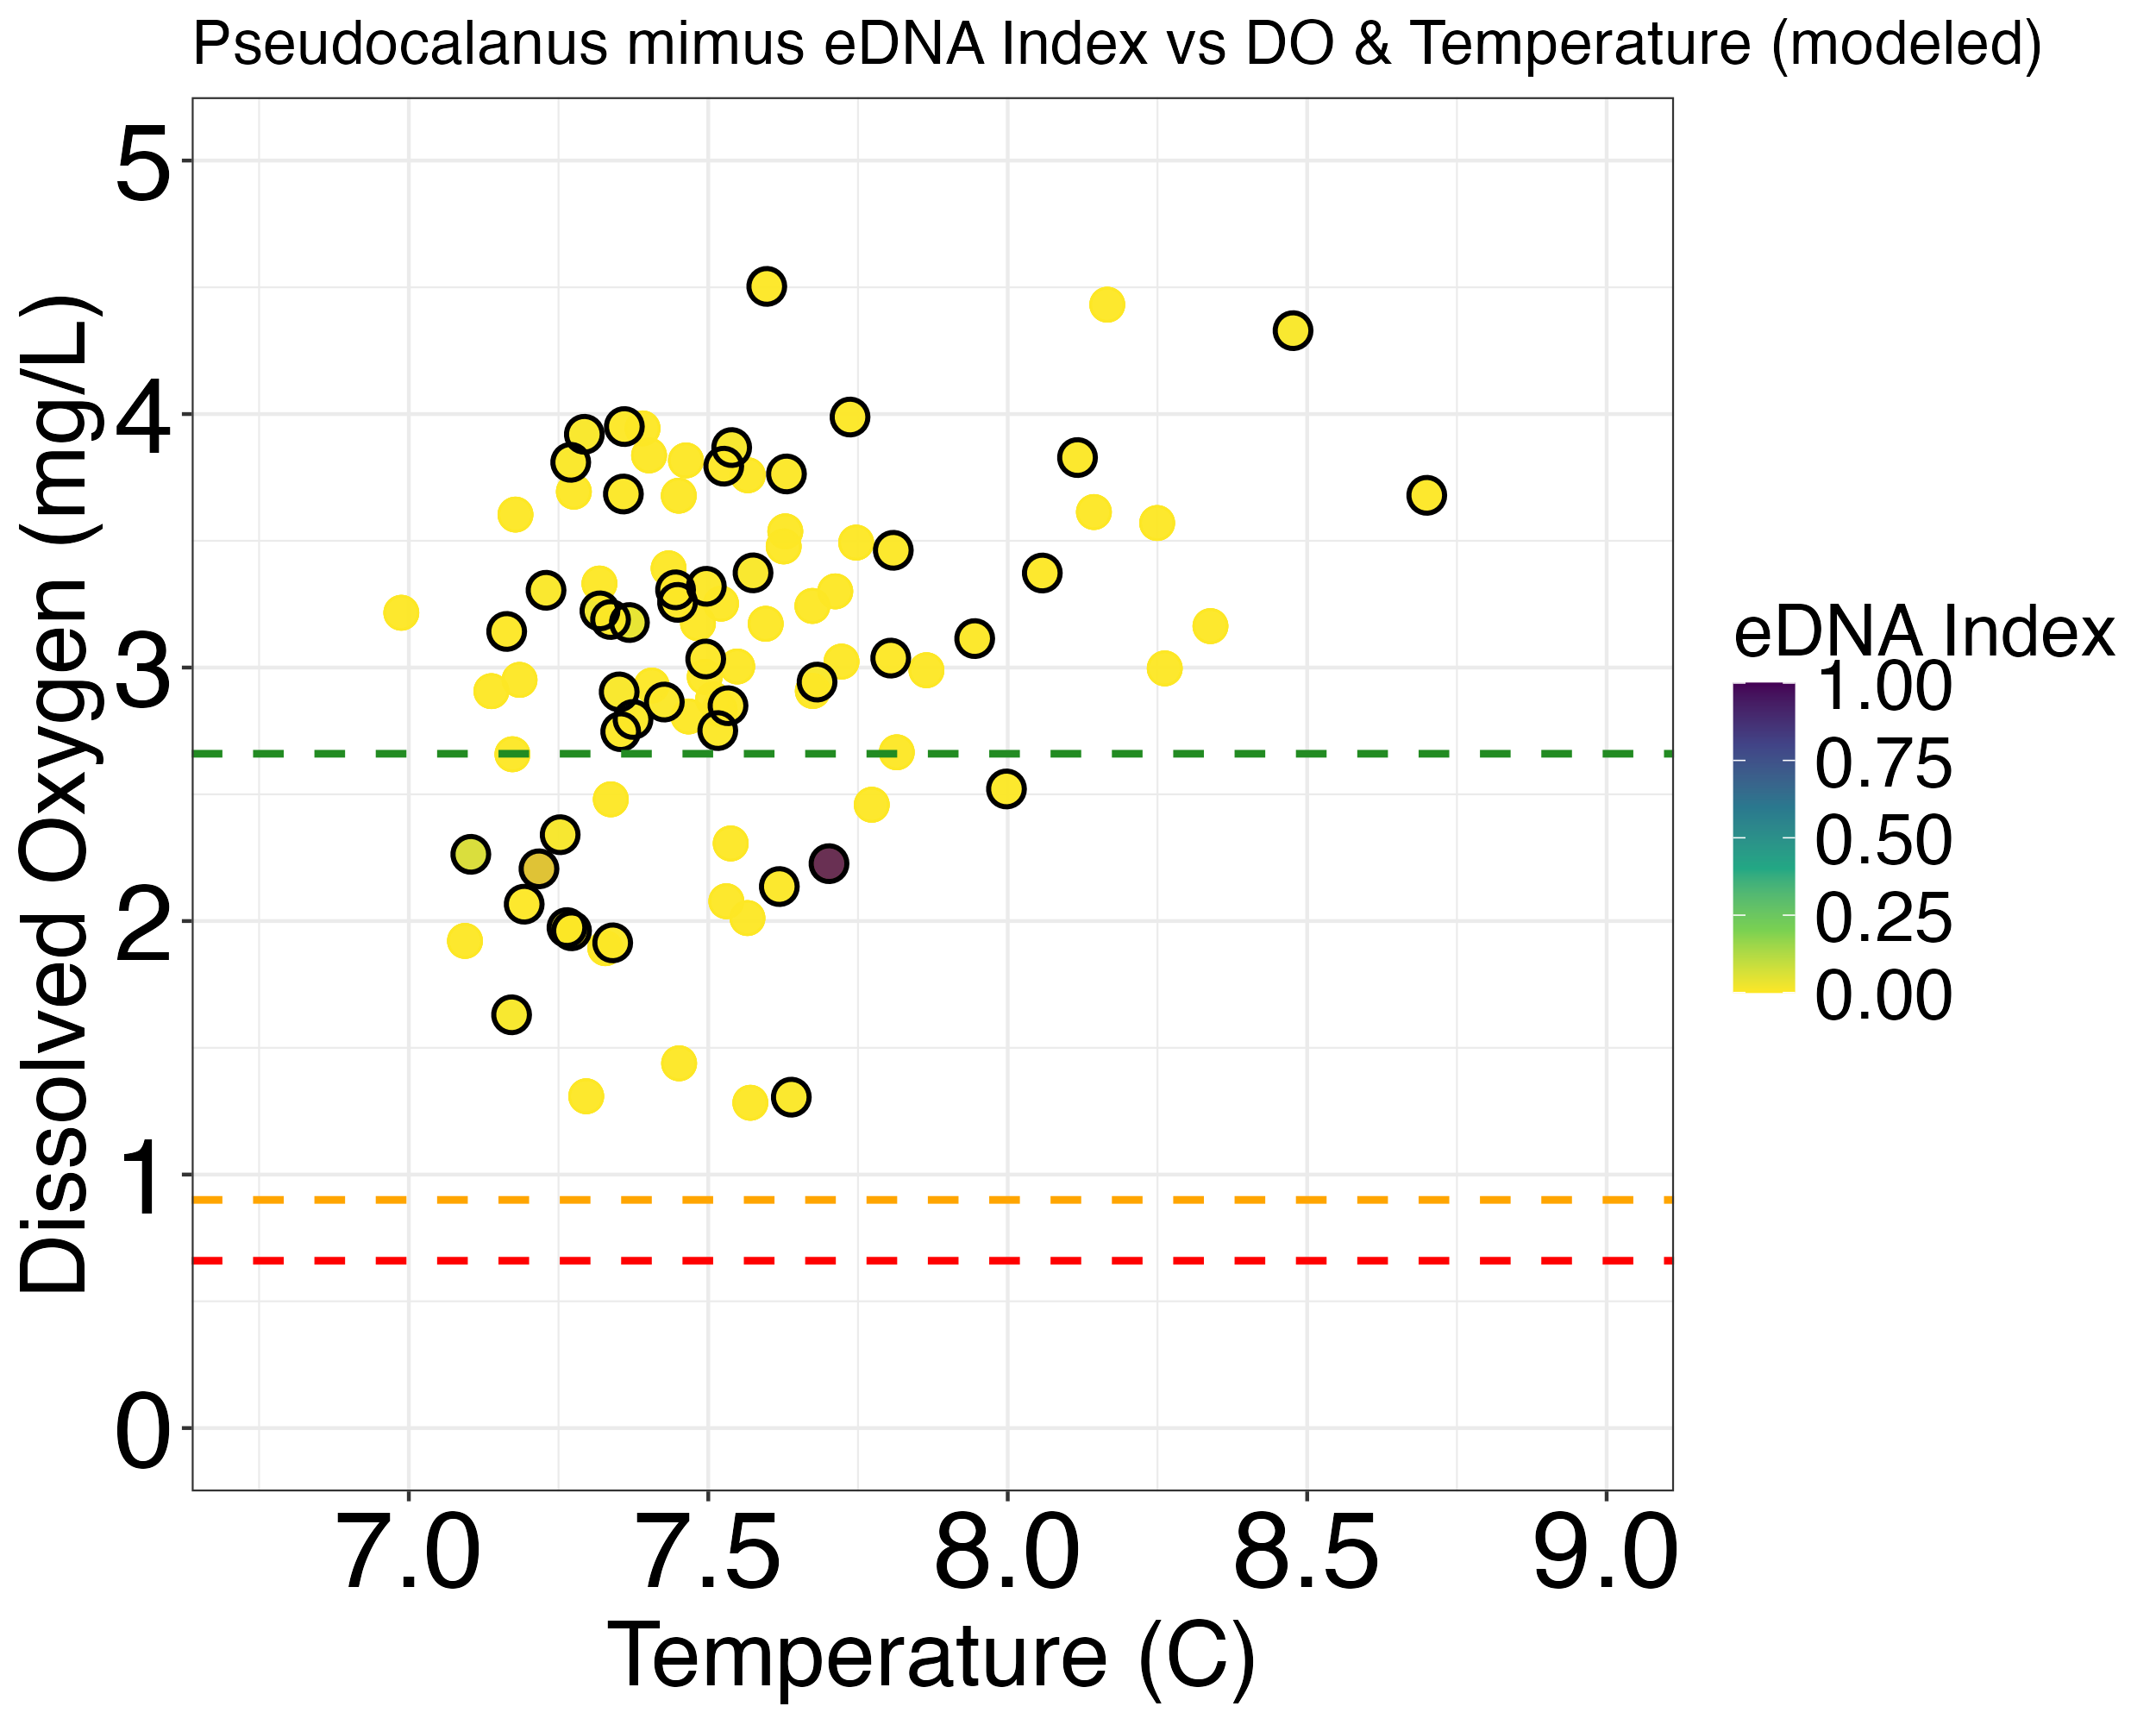
\includegraphics[scale=0.3]{Pmimus_Scatter_AllYr_mod_noOut}
			\caption[\textit{P. mimus} scatterplot]{\footnotesize{Scatterplot of dissolved oxygen (mg/L) and temperature (Celsius) for each environmental DNA sampling time, with \textit{P. mimus} detections circled in black. Color of dots represents eDNA index, a normalized measure of abundance that can compare abundance within a species. Yellow, uncircled dots represent sampling dates when \textit{P. mimus} was not detected. Plot (a) uses TH042 mooring data from 2021-22, (b) uses LiveOcean model data from 2021-23.}} %the special ToC caption is in square brackets. The \footnotesize makes the figure caption smaller
			\label{PmimusScatter}
			\end{center}
	\end{figure} 
	
	\begin{figure}[!h]
		\begin{center}
			%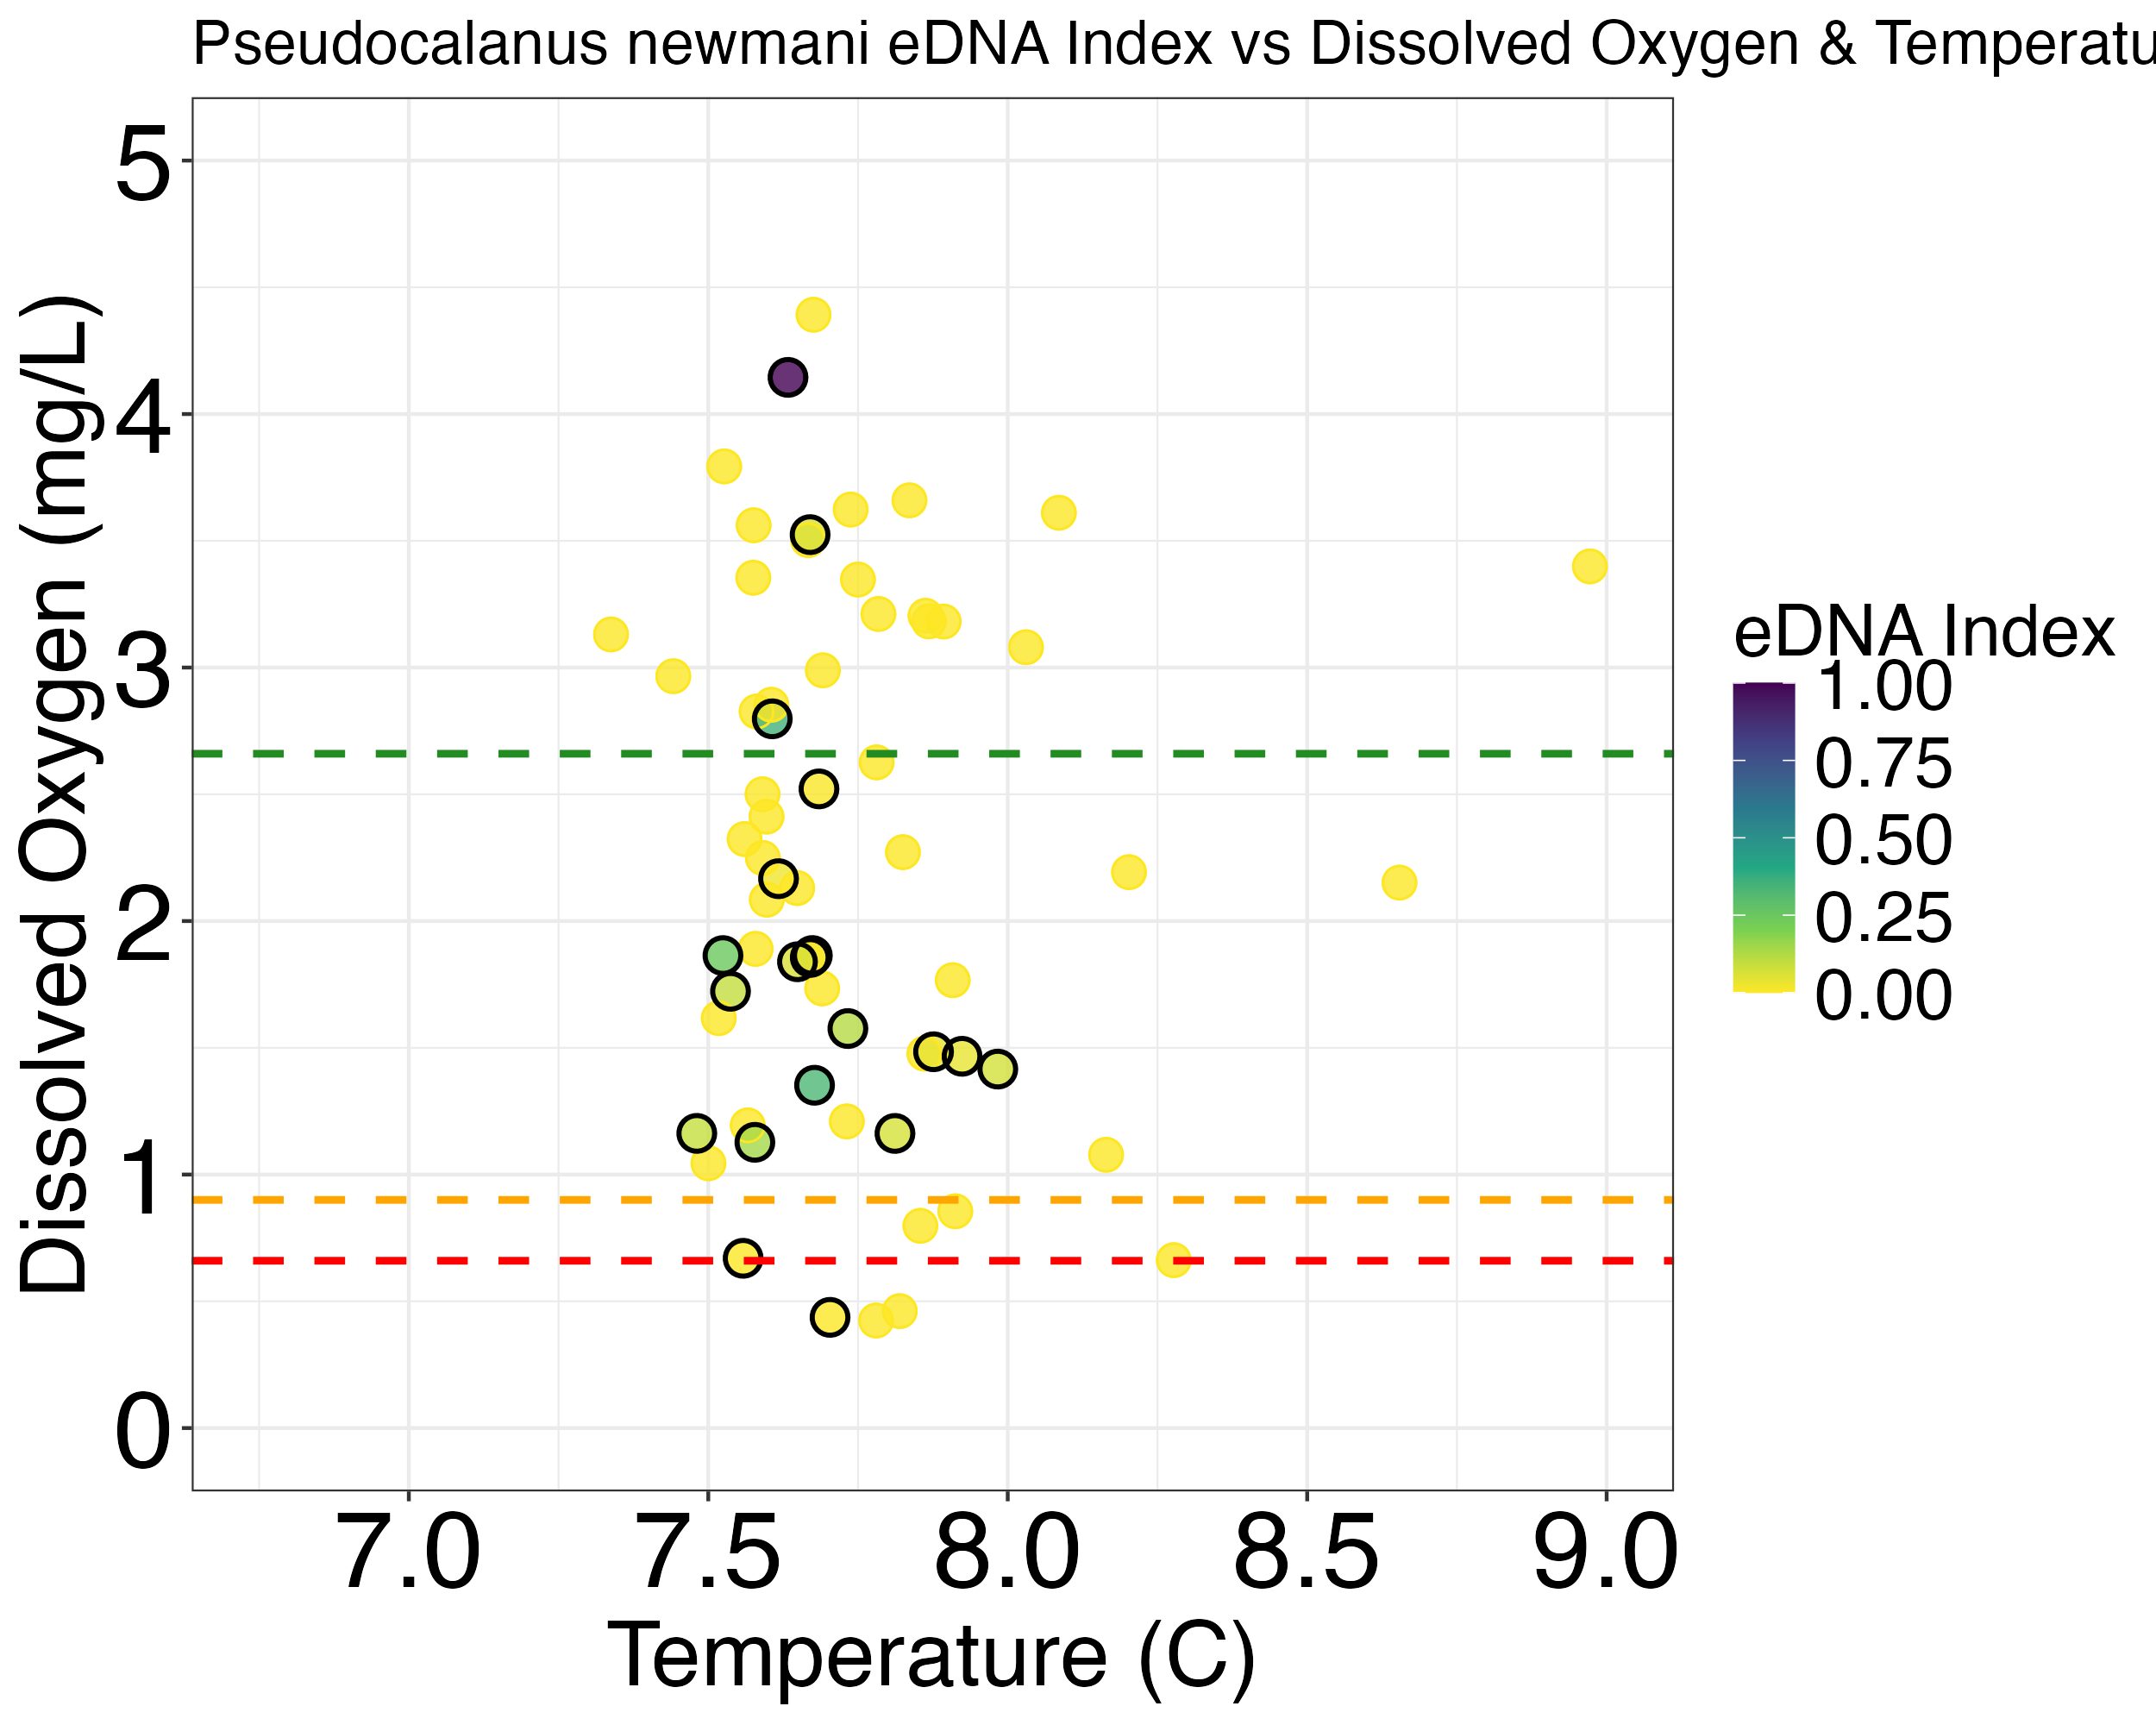
\includegraphics[scale=0.35]{Pnewmani_Scatter_noOut}
			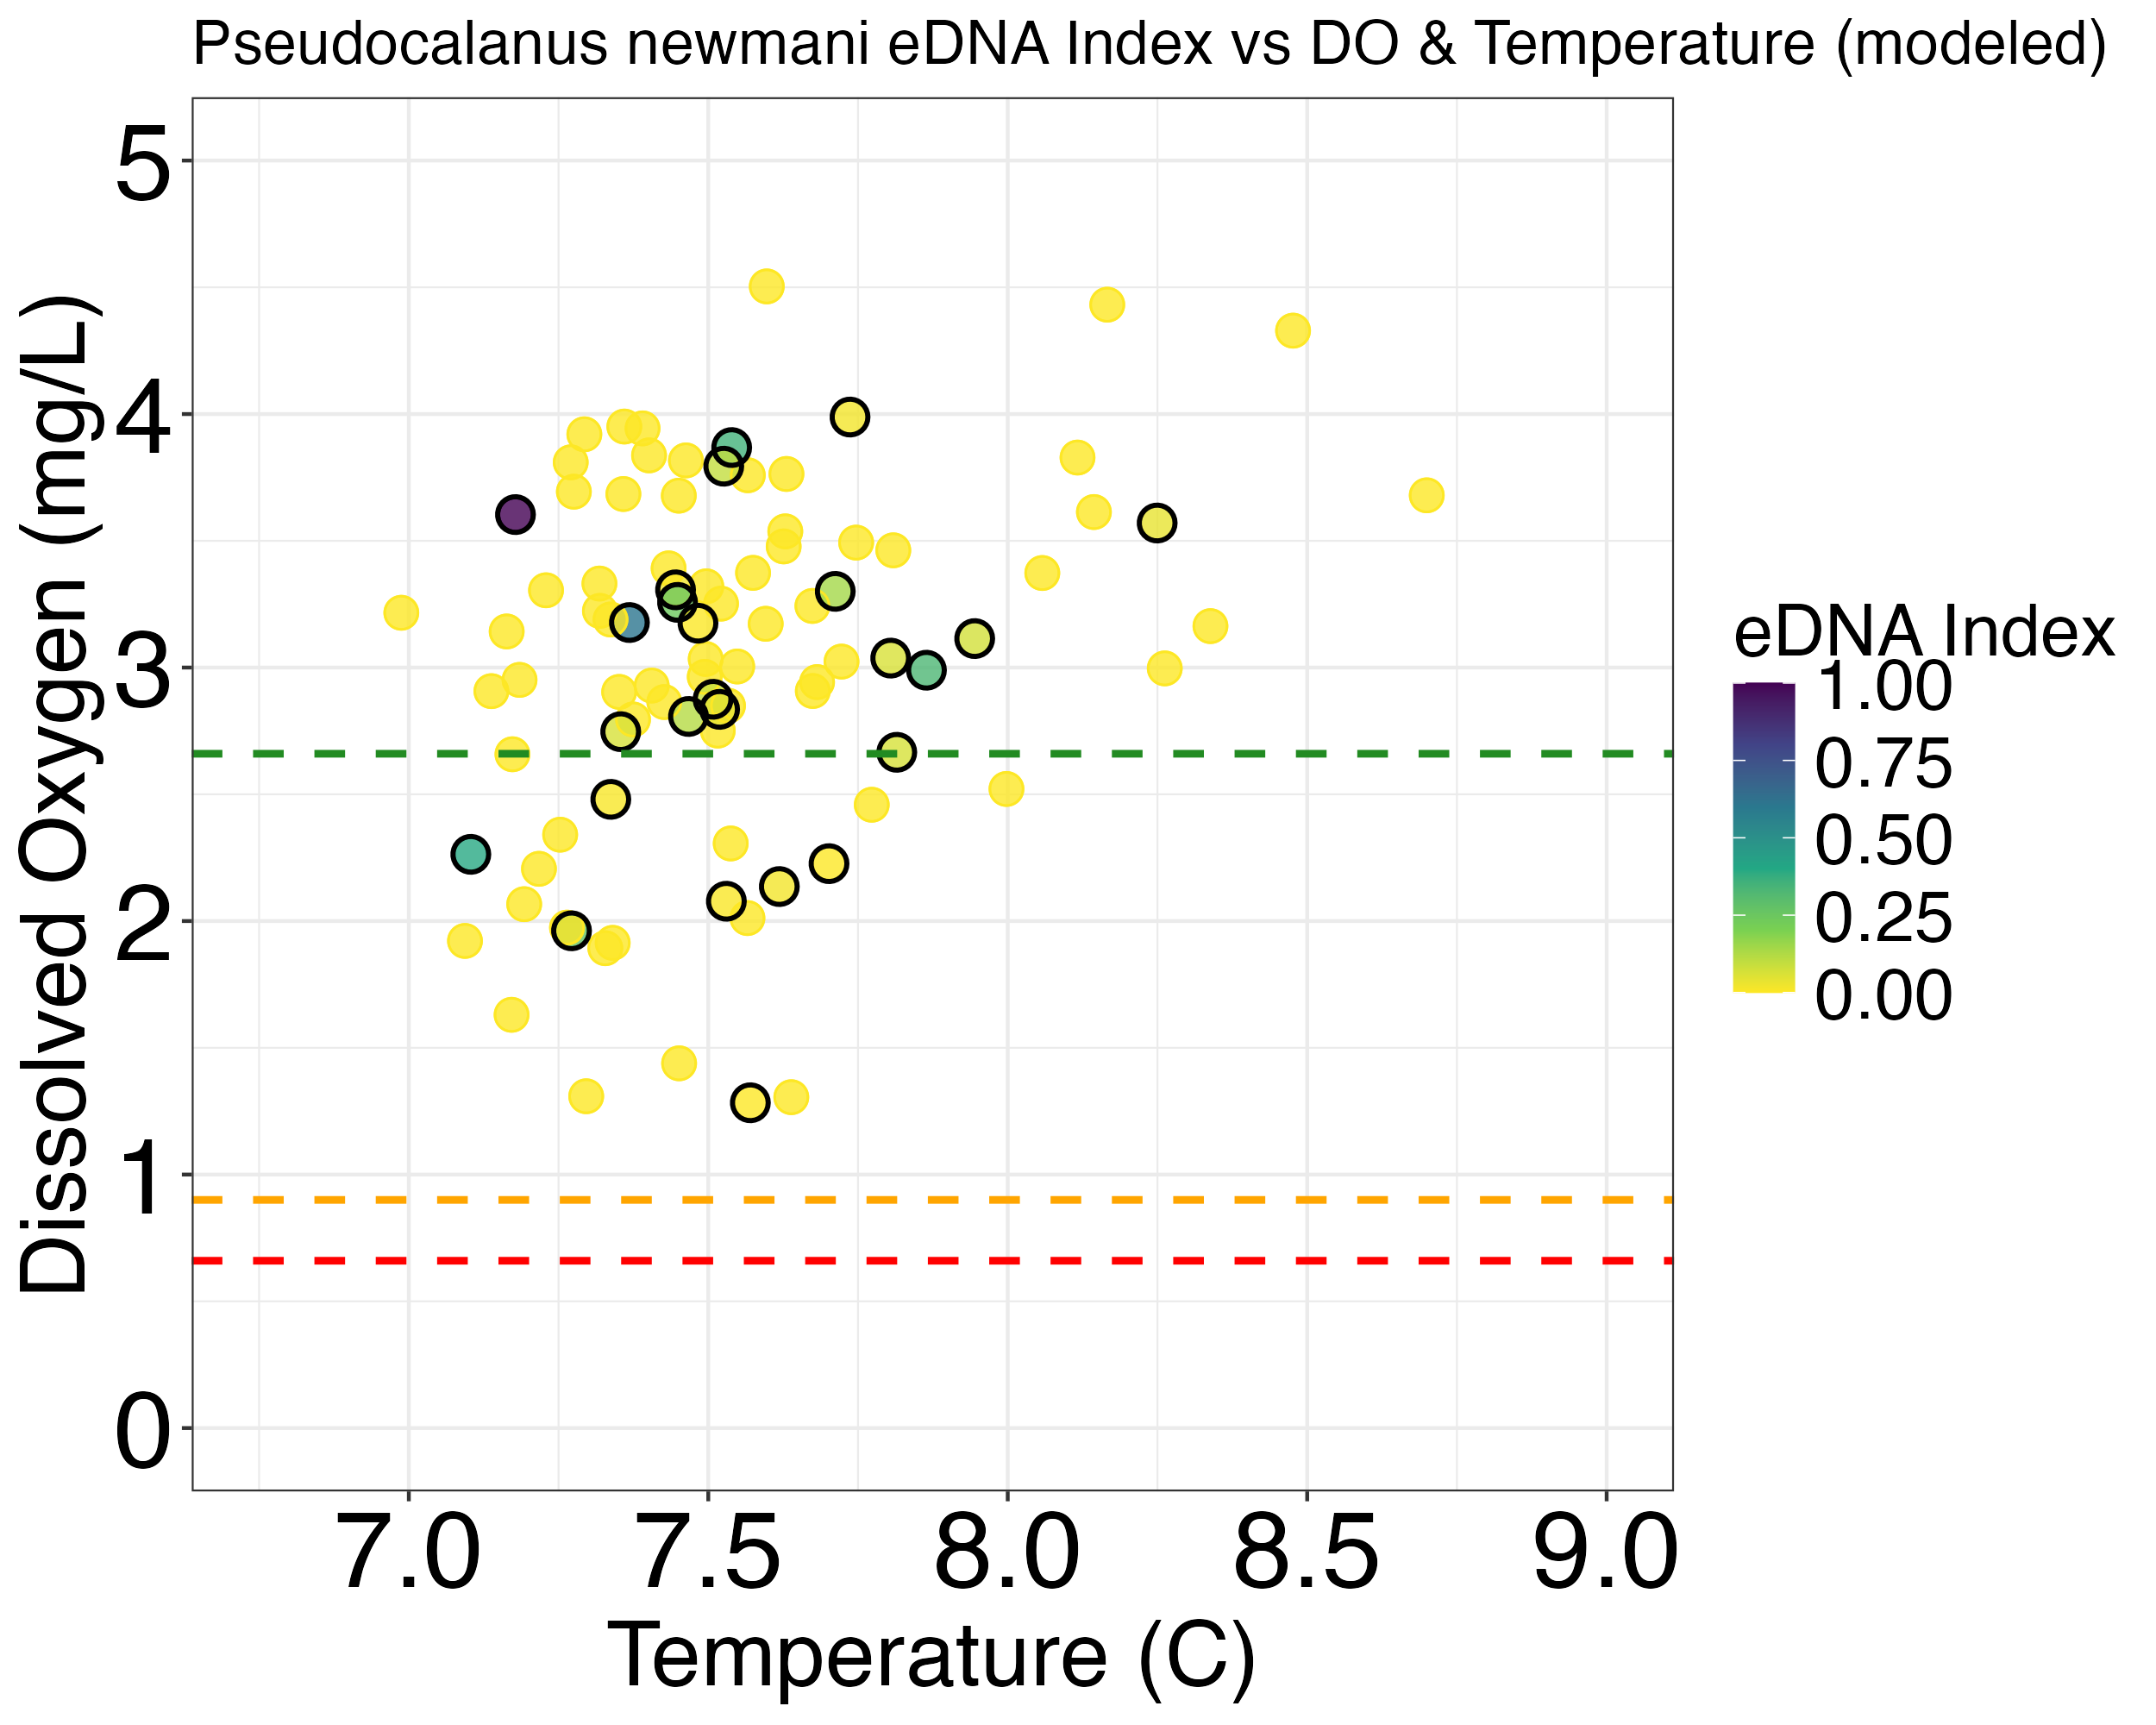
\includegraphics[scale=0.3]{Pnewmani_Scatter_AllYr_mod_noOut}
			\caption[\textit{P. newmani} scatterplot]{\footnotesize{Scatterplot of dissolved oxygen (mg/L) and temperature (Celsius) for each environmental DNA sampling time, with \textit{P. newmani} detections circled in black. Color of dots represents eDNA index, a normalized measure of abundance that can compare abundance within a species. Yellow, uncircled dots represent sampling dates when \textit{P. newmani} was not detected. This plot uses LiveOcean model data from 2021-23.}} %the special ToC caption is in square brackets. The \footnotesize makes the figure caption smaller
			\label{PnewmaniScatter}
		\end{center}
	\end{figure} 
	
	\begin{figure}[!h]
		\begin{center}
			a. 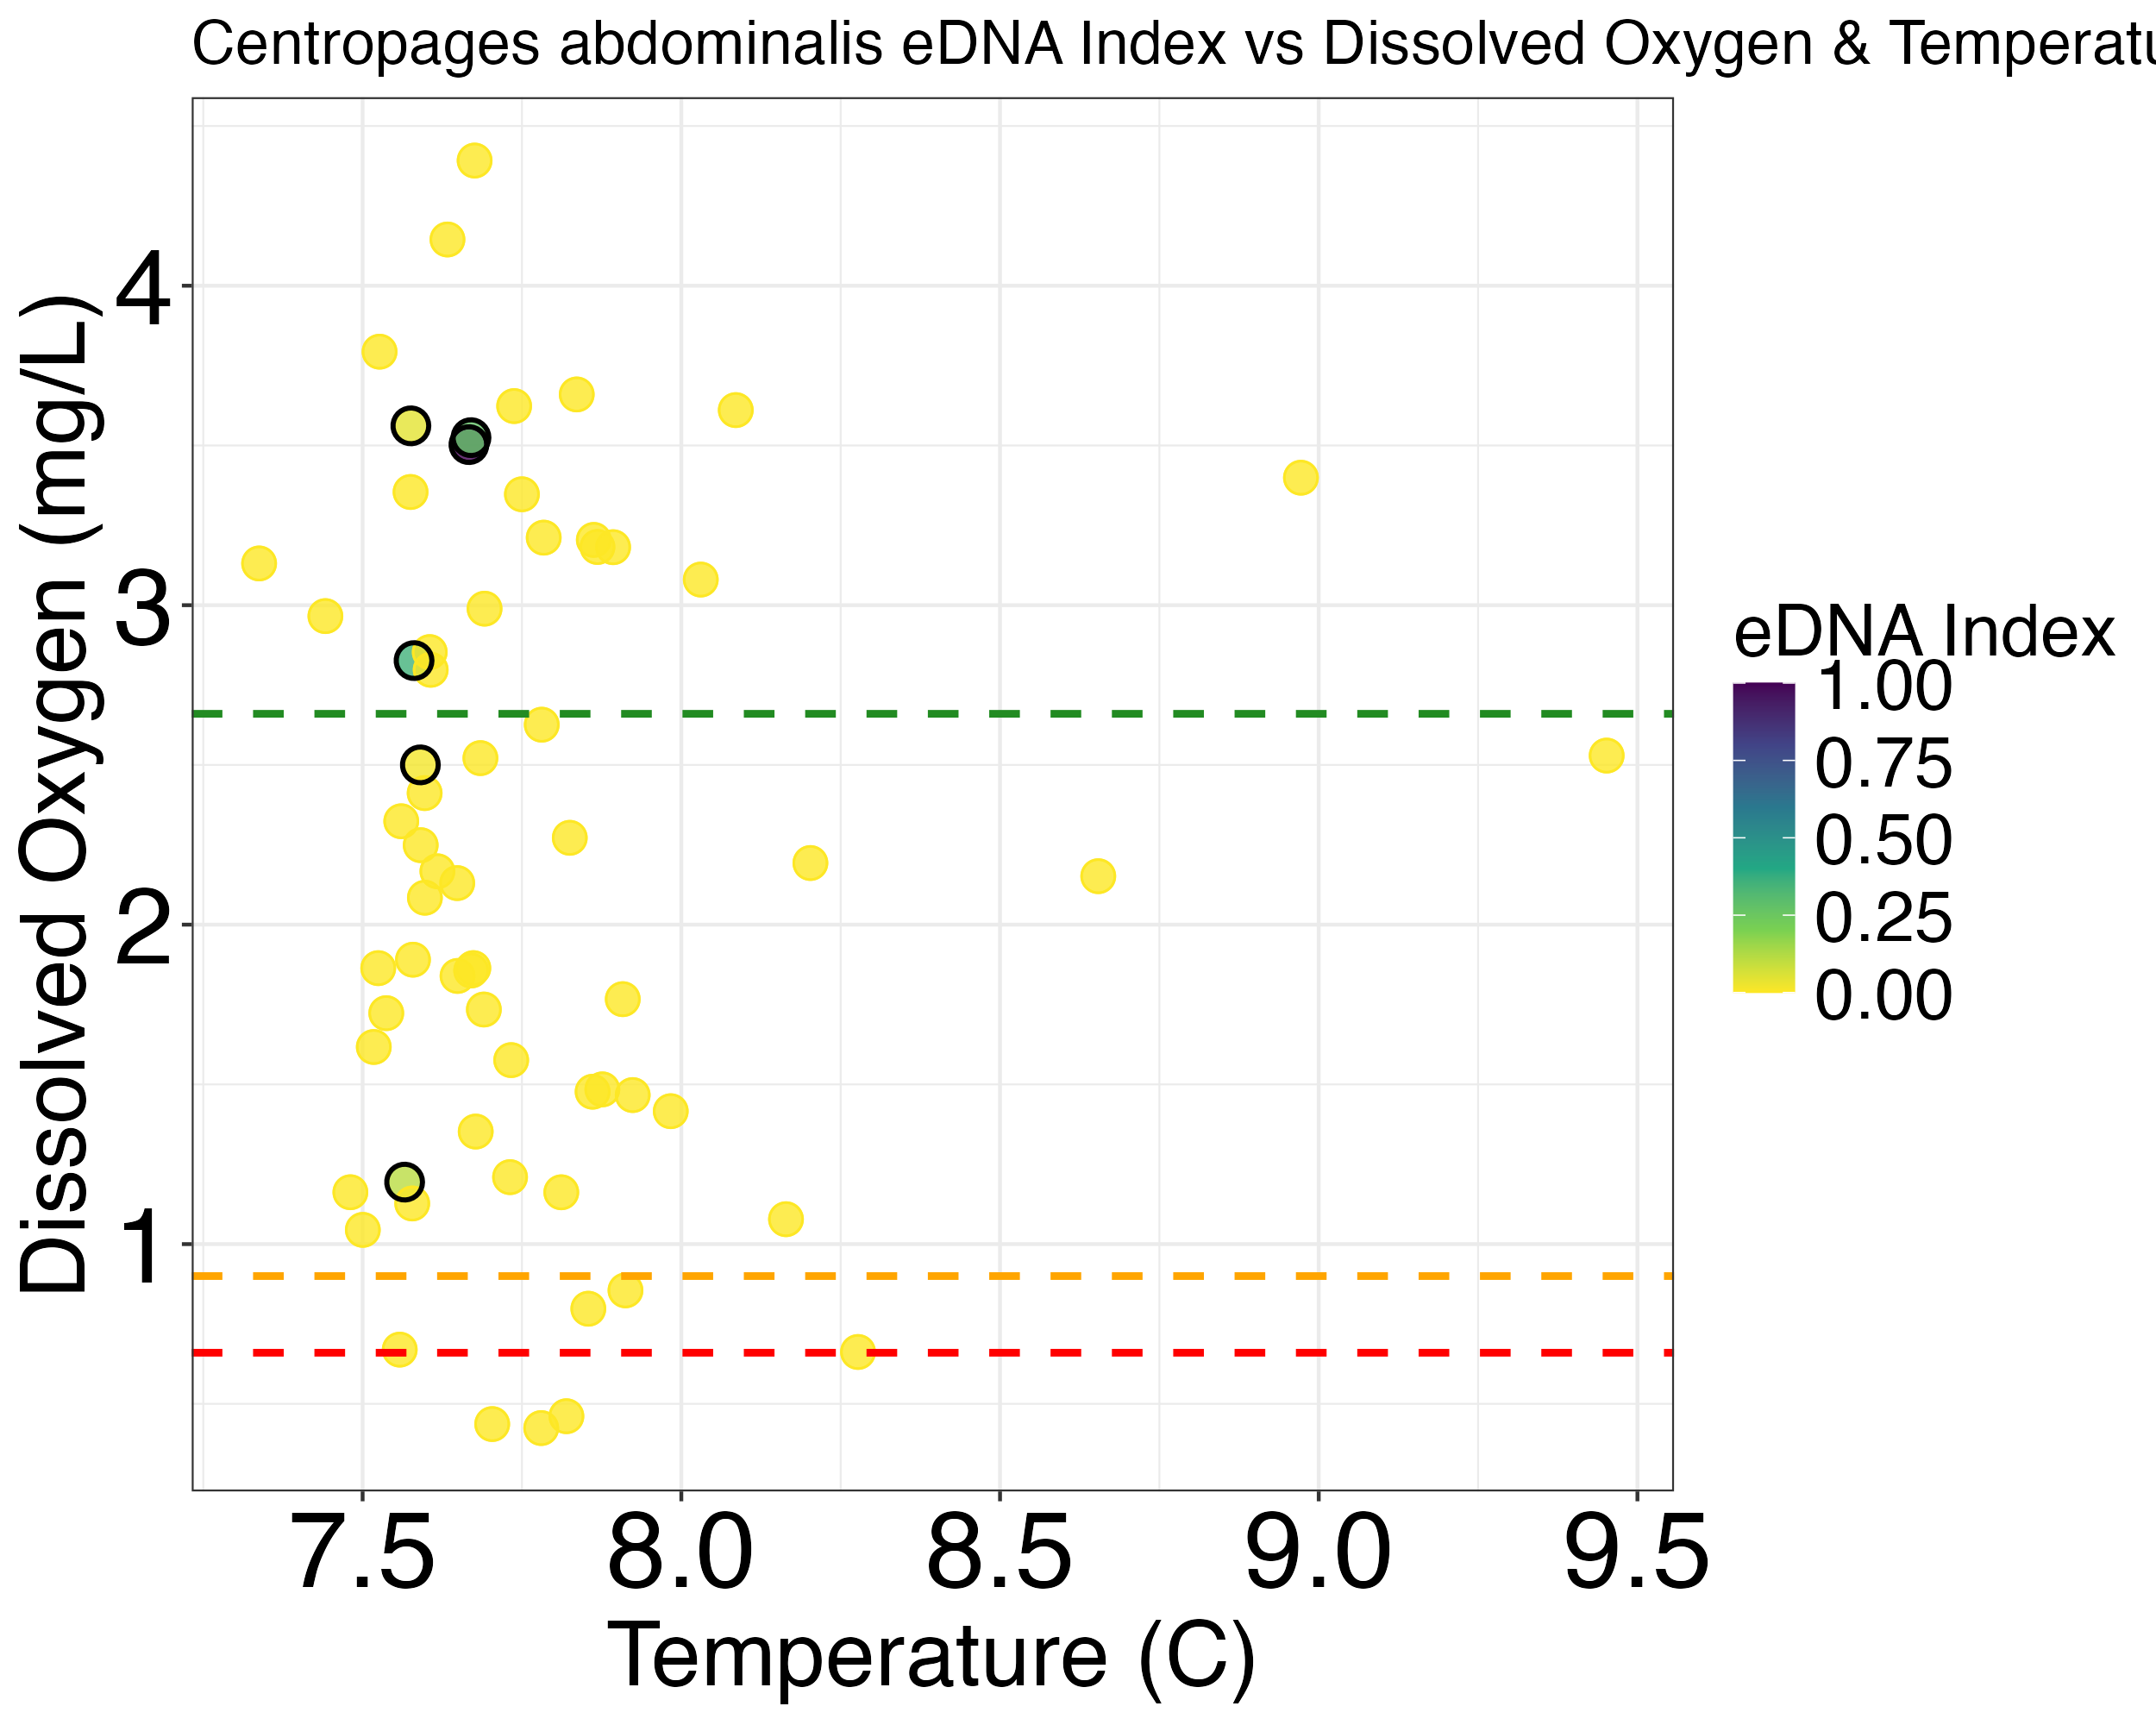
\includegraphics[scale=0.3]{Cabdominalis_Scatter_noOut}
			b. 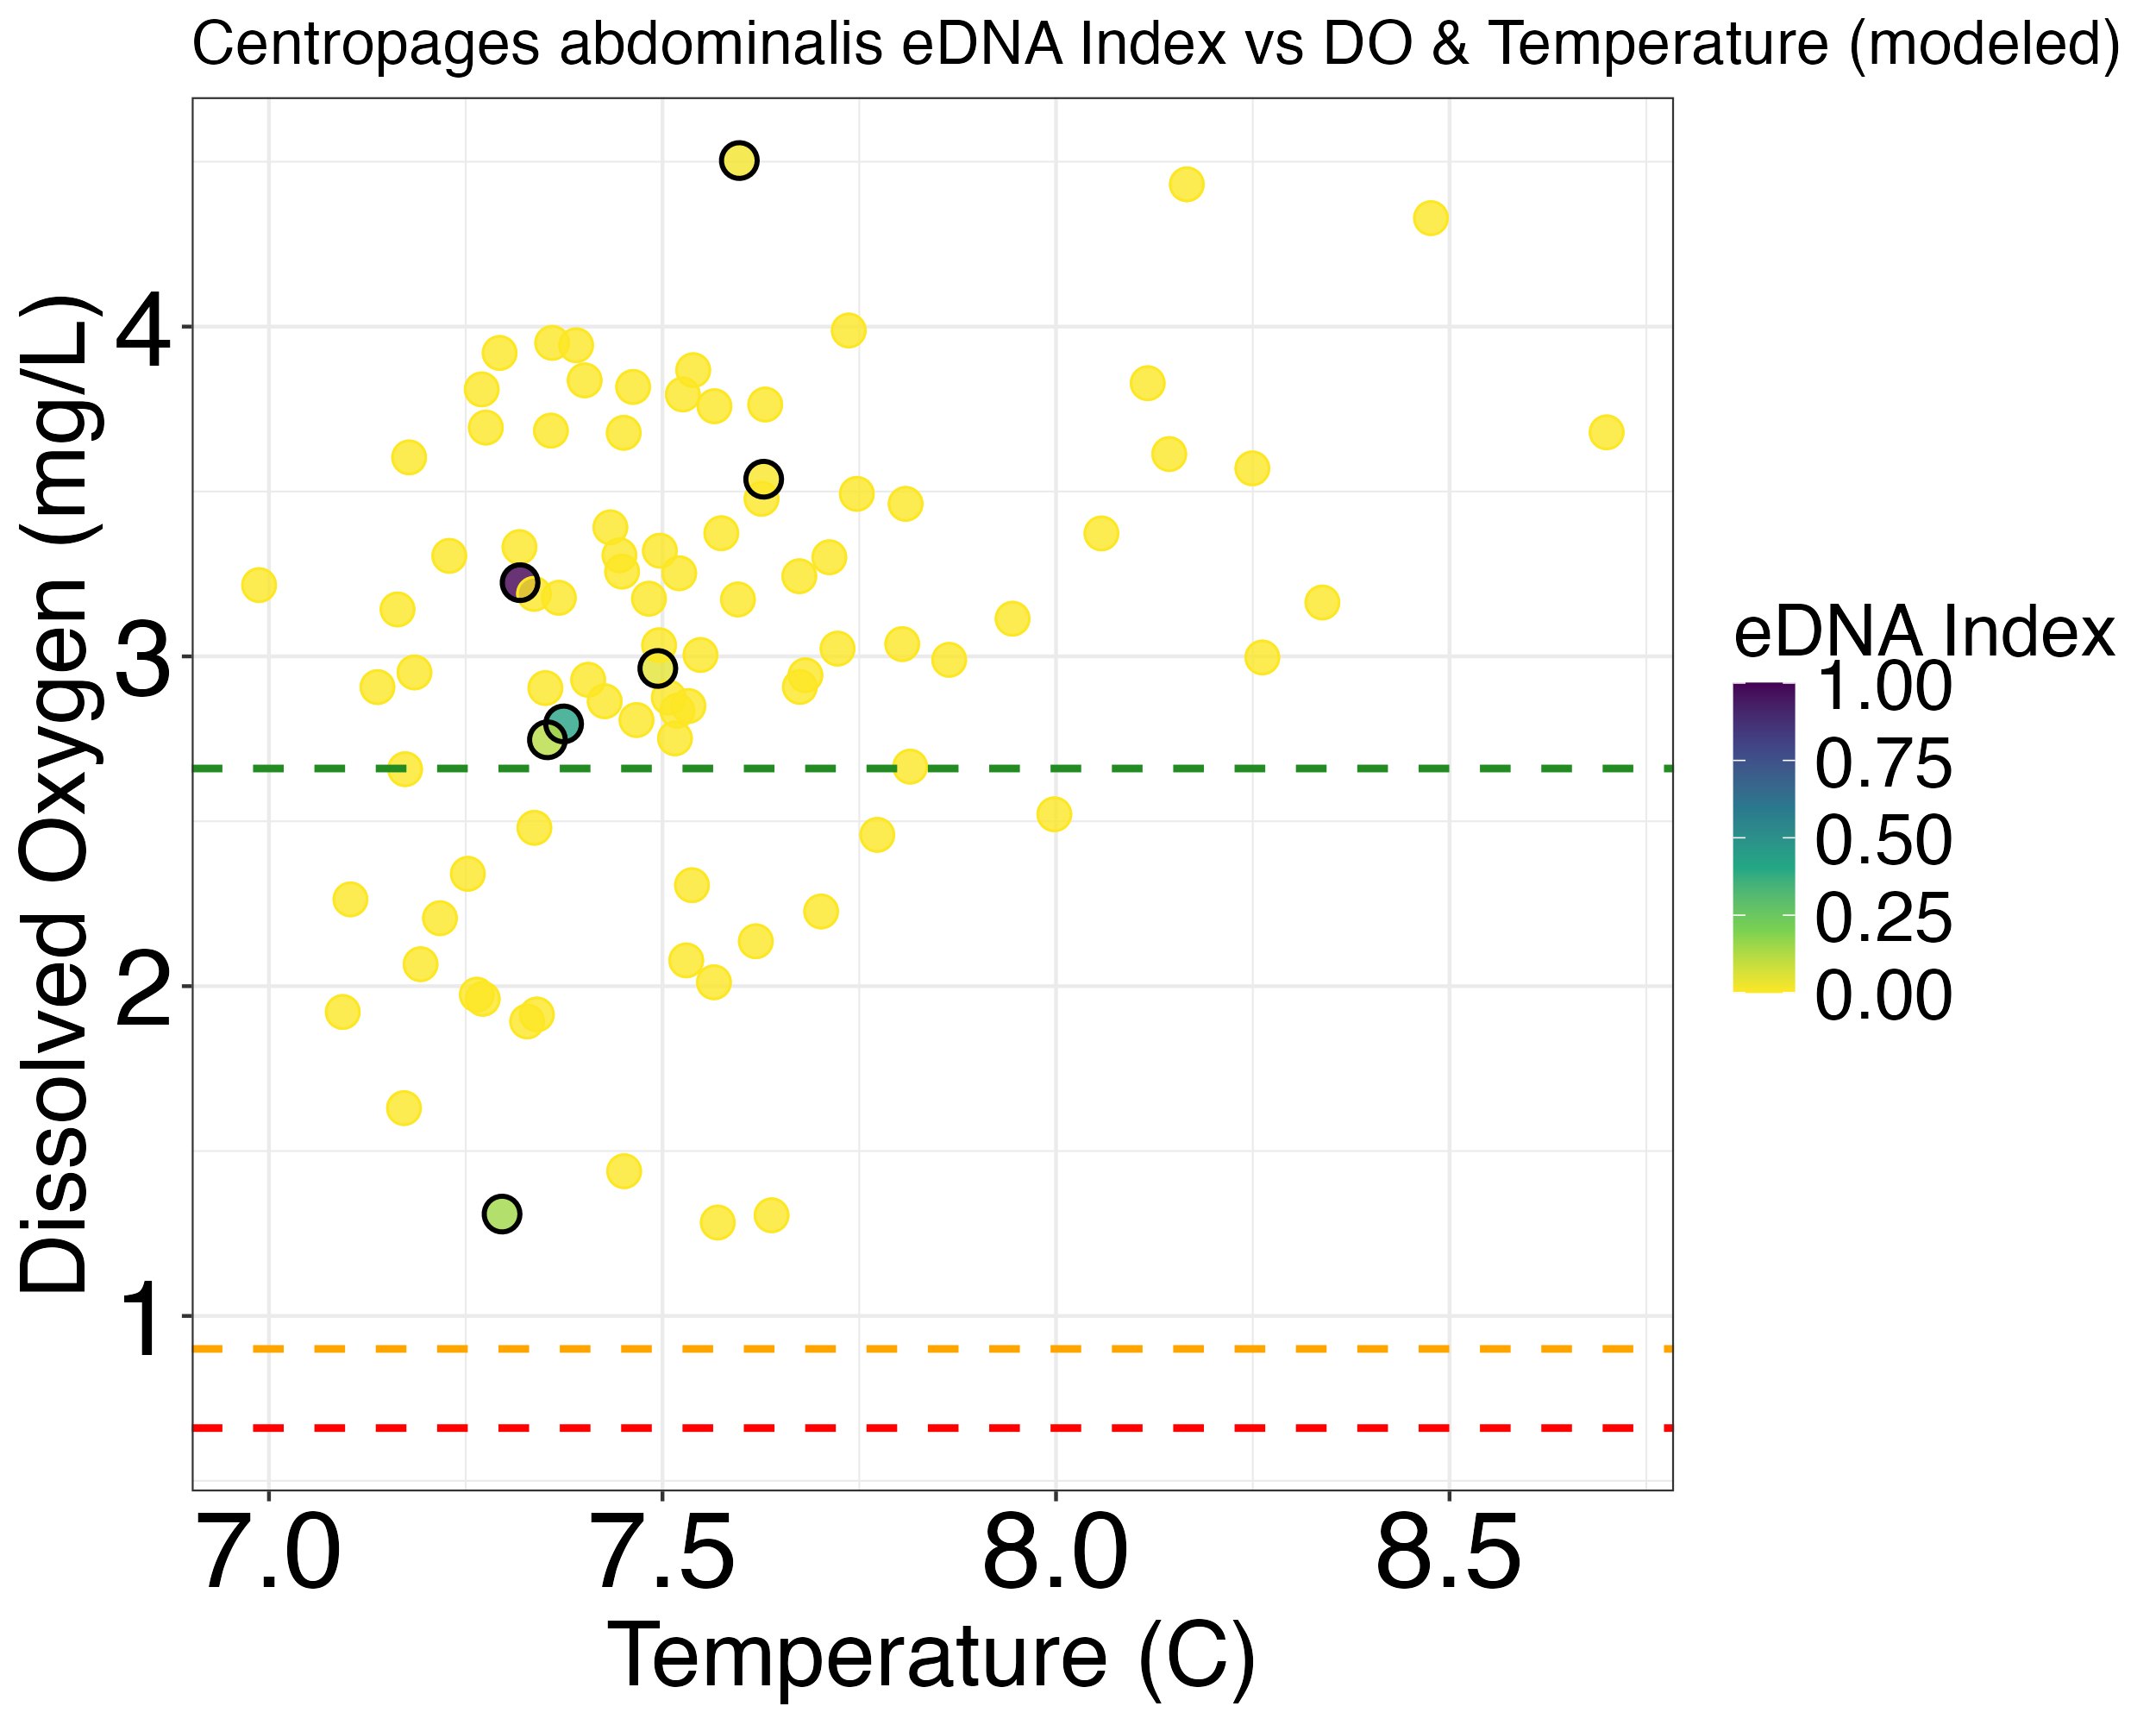
\includegraphics[scale=0.3]{Cabdominalis_Scatter_AllYr_mod_noOut}
			\caption[\textit{C. abdominalis} scatterplot]{\footnotesize{Scatterplot of dissolved oxygen (mg/L) and temperature (Celsius) for each environmental DNA sampling time, with \textit{C. abdominalis} detections circled in black. Color of dots represents eDNA index, a normalized measure of abundance that can compare abundance within a species. Yellow, uncircled dots represent sampling dates when \textit{C. abdominalis} was not detected. Plot (a) uses TH042 mooring data from 2021-22, (b) uses LiveOcean model data from 2021-23.}} %the special ToC caption is in square brackets. The \footnotesize makes the figure caption smaller
			\label{CabdominalisScatter}
		\end{center}
	\end{figure} 
	
	\begin{figure}[!h]
		\begin{center}
			a. 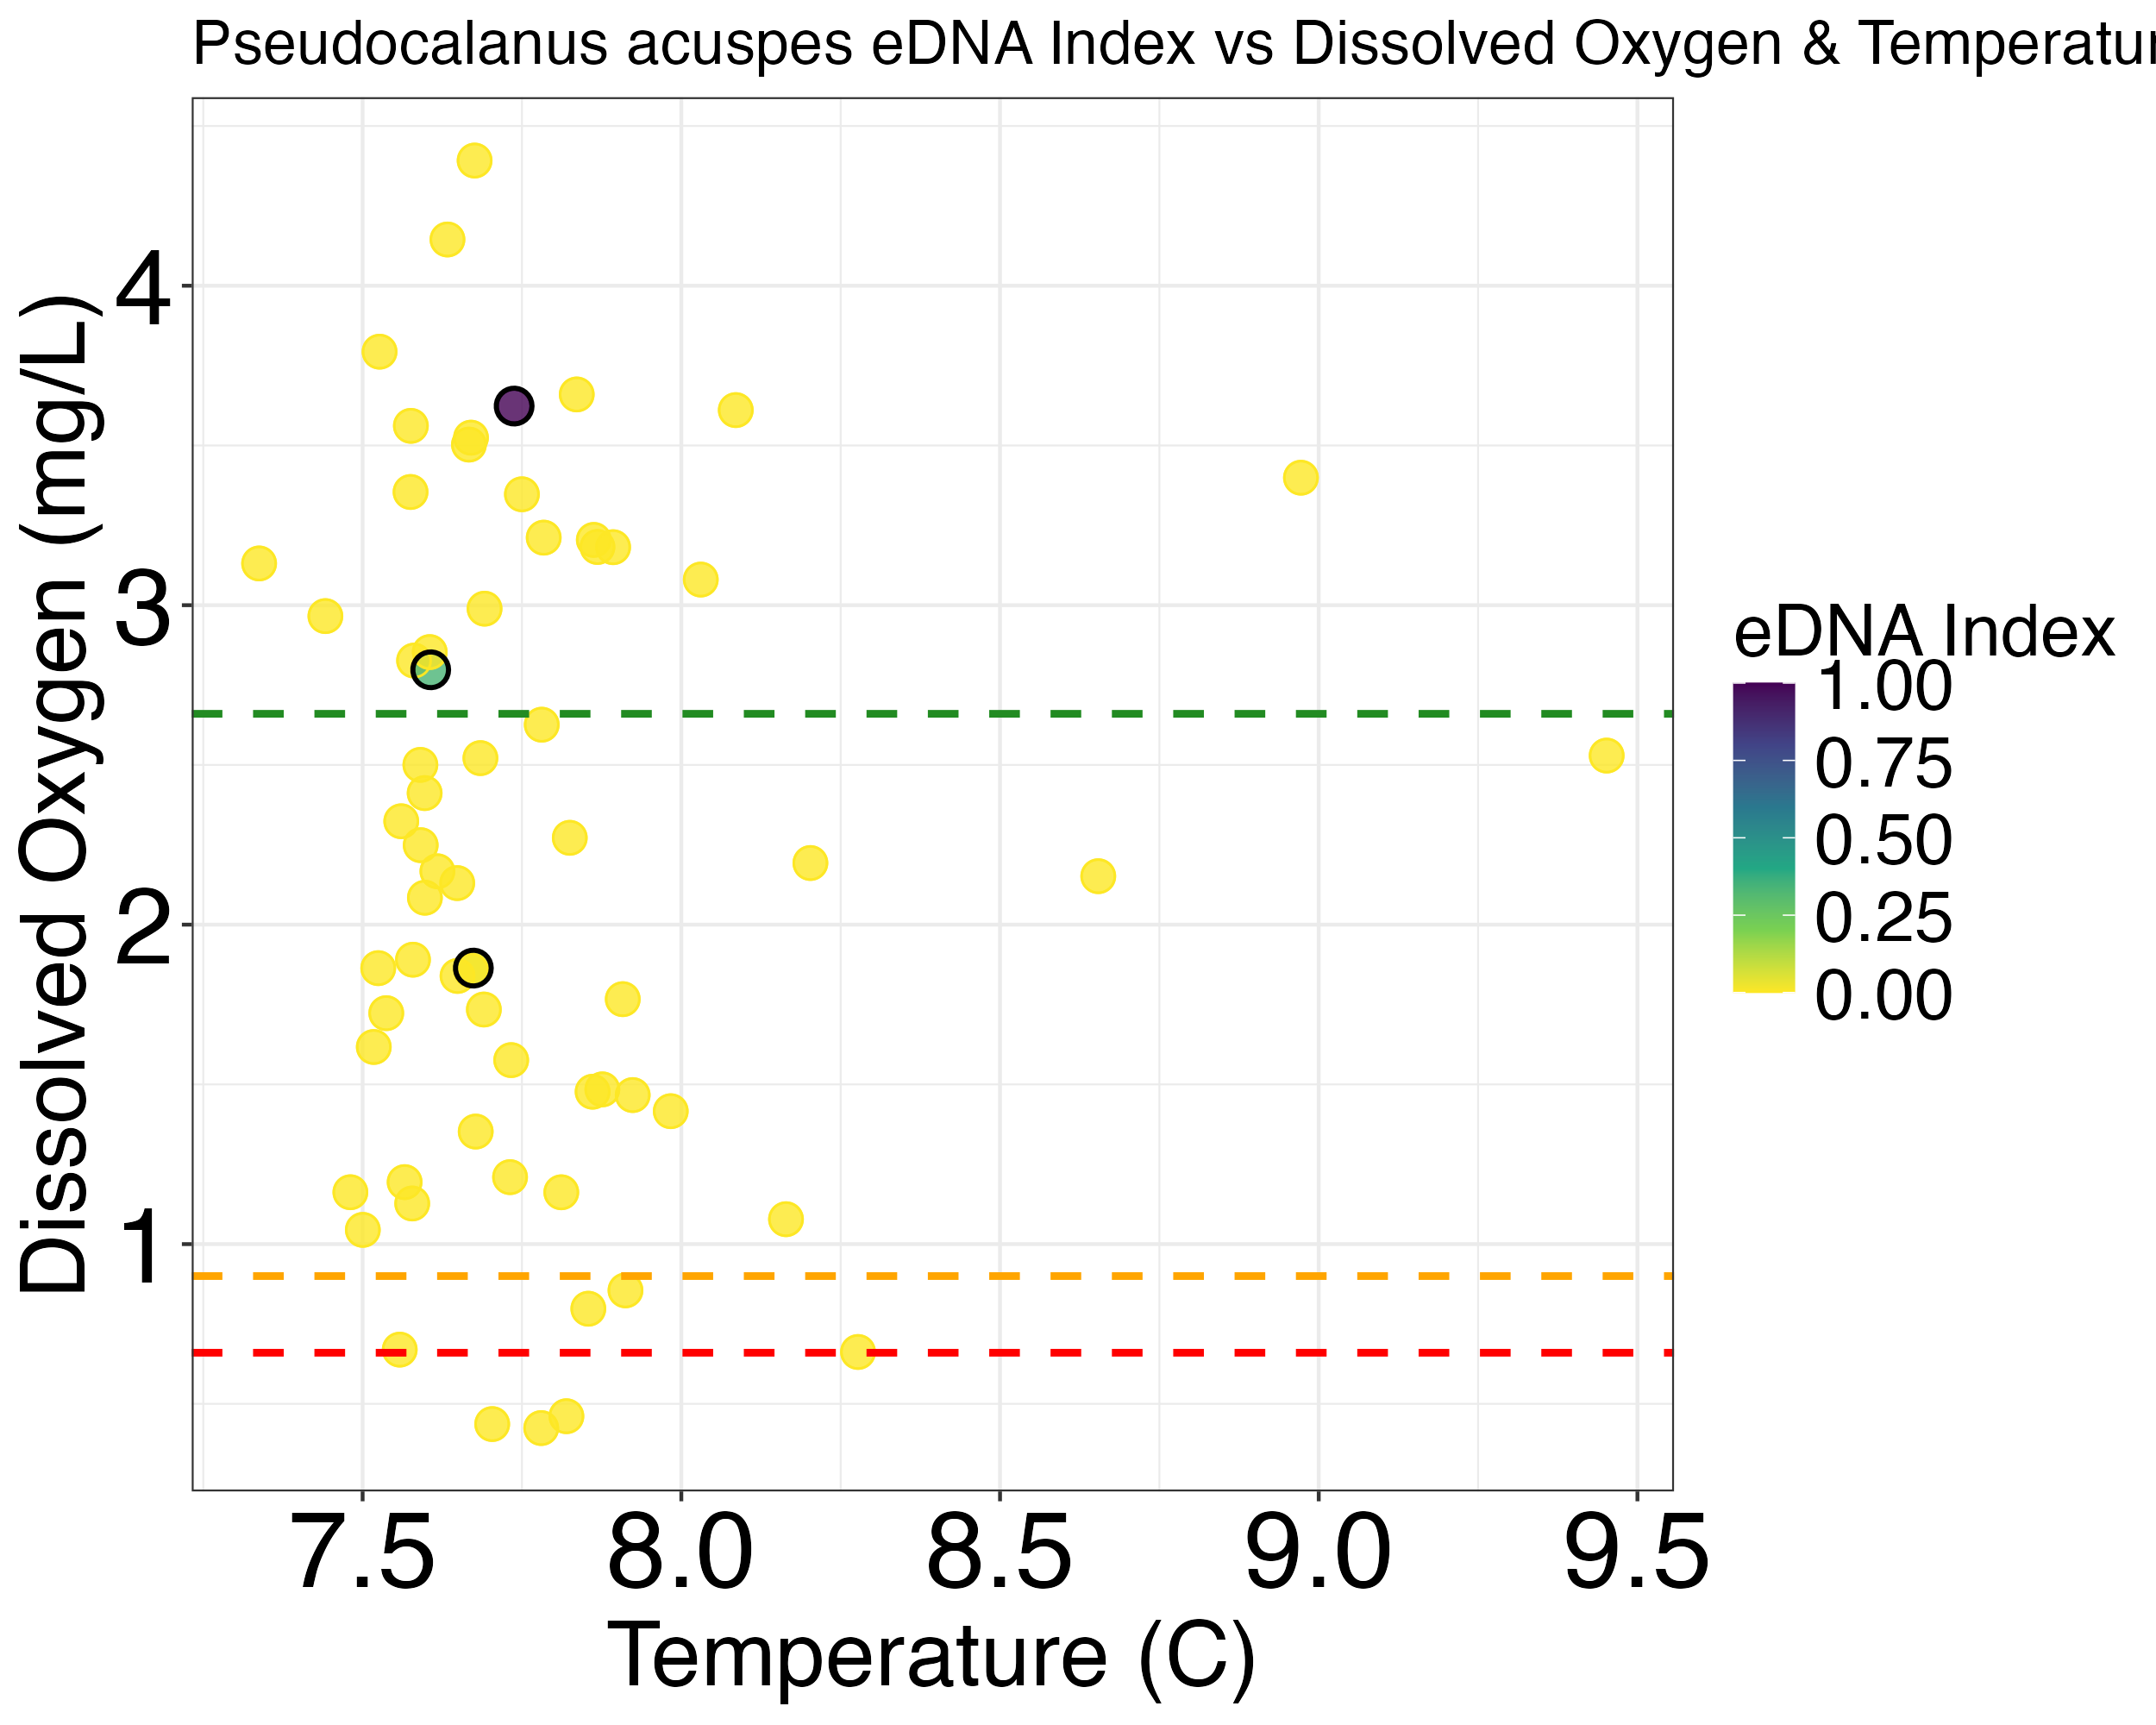
\includegraphics[scale=0.3]{Pacuspes_Scatter_noOut}
			b. 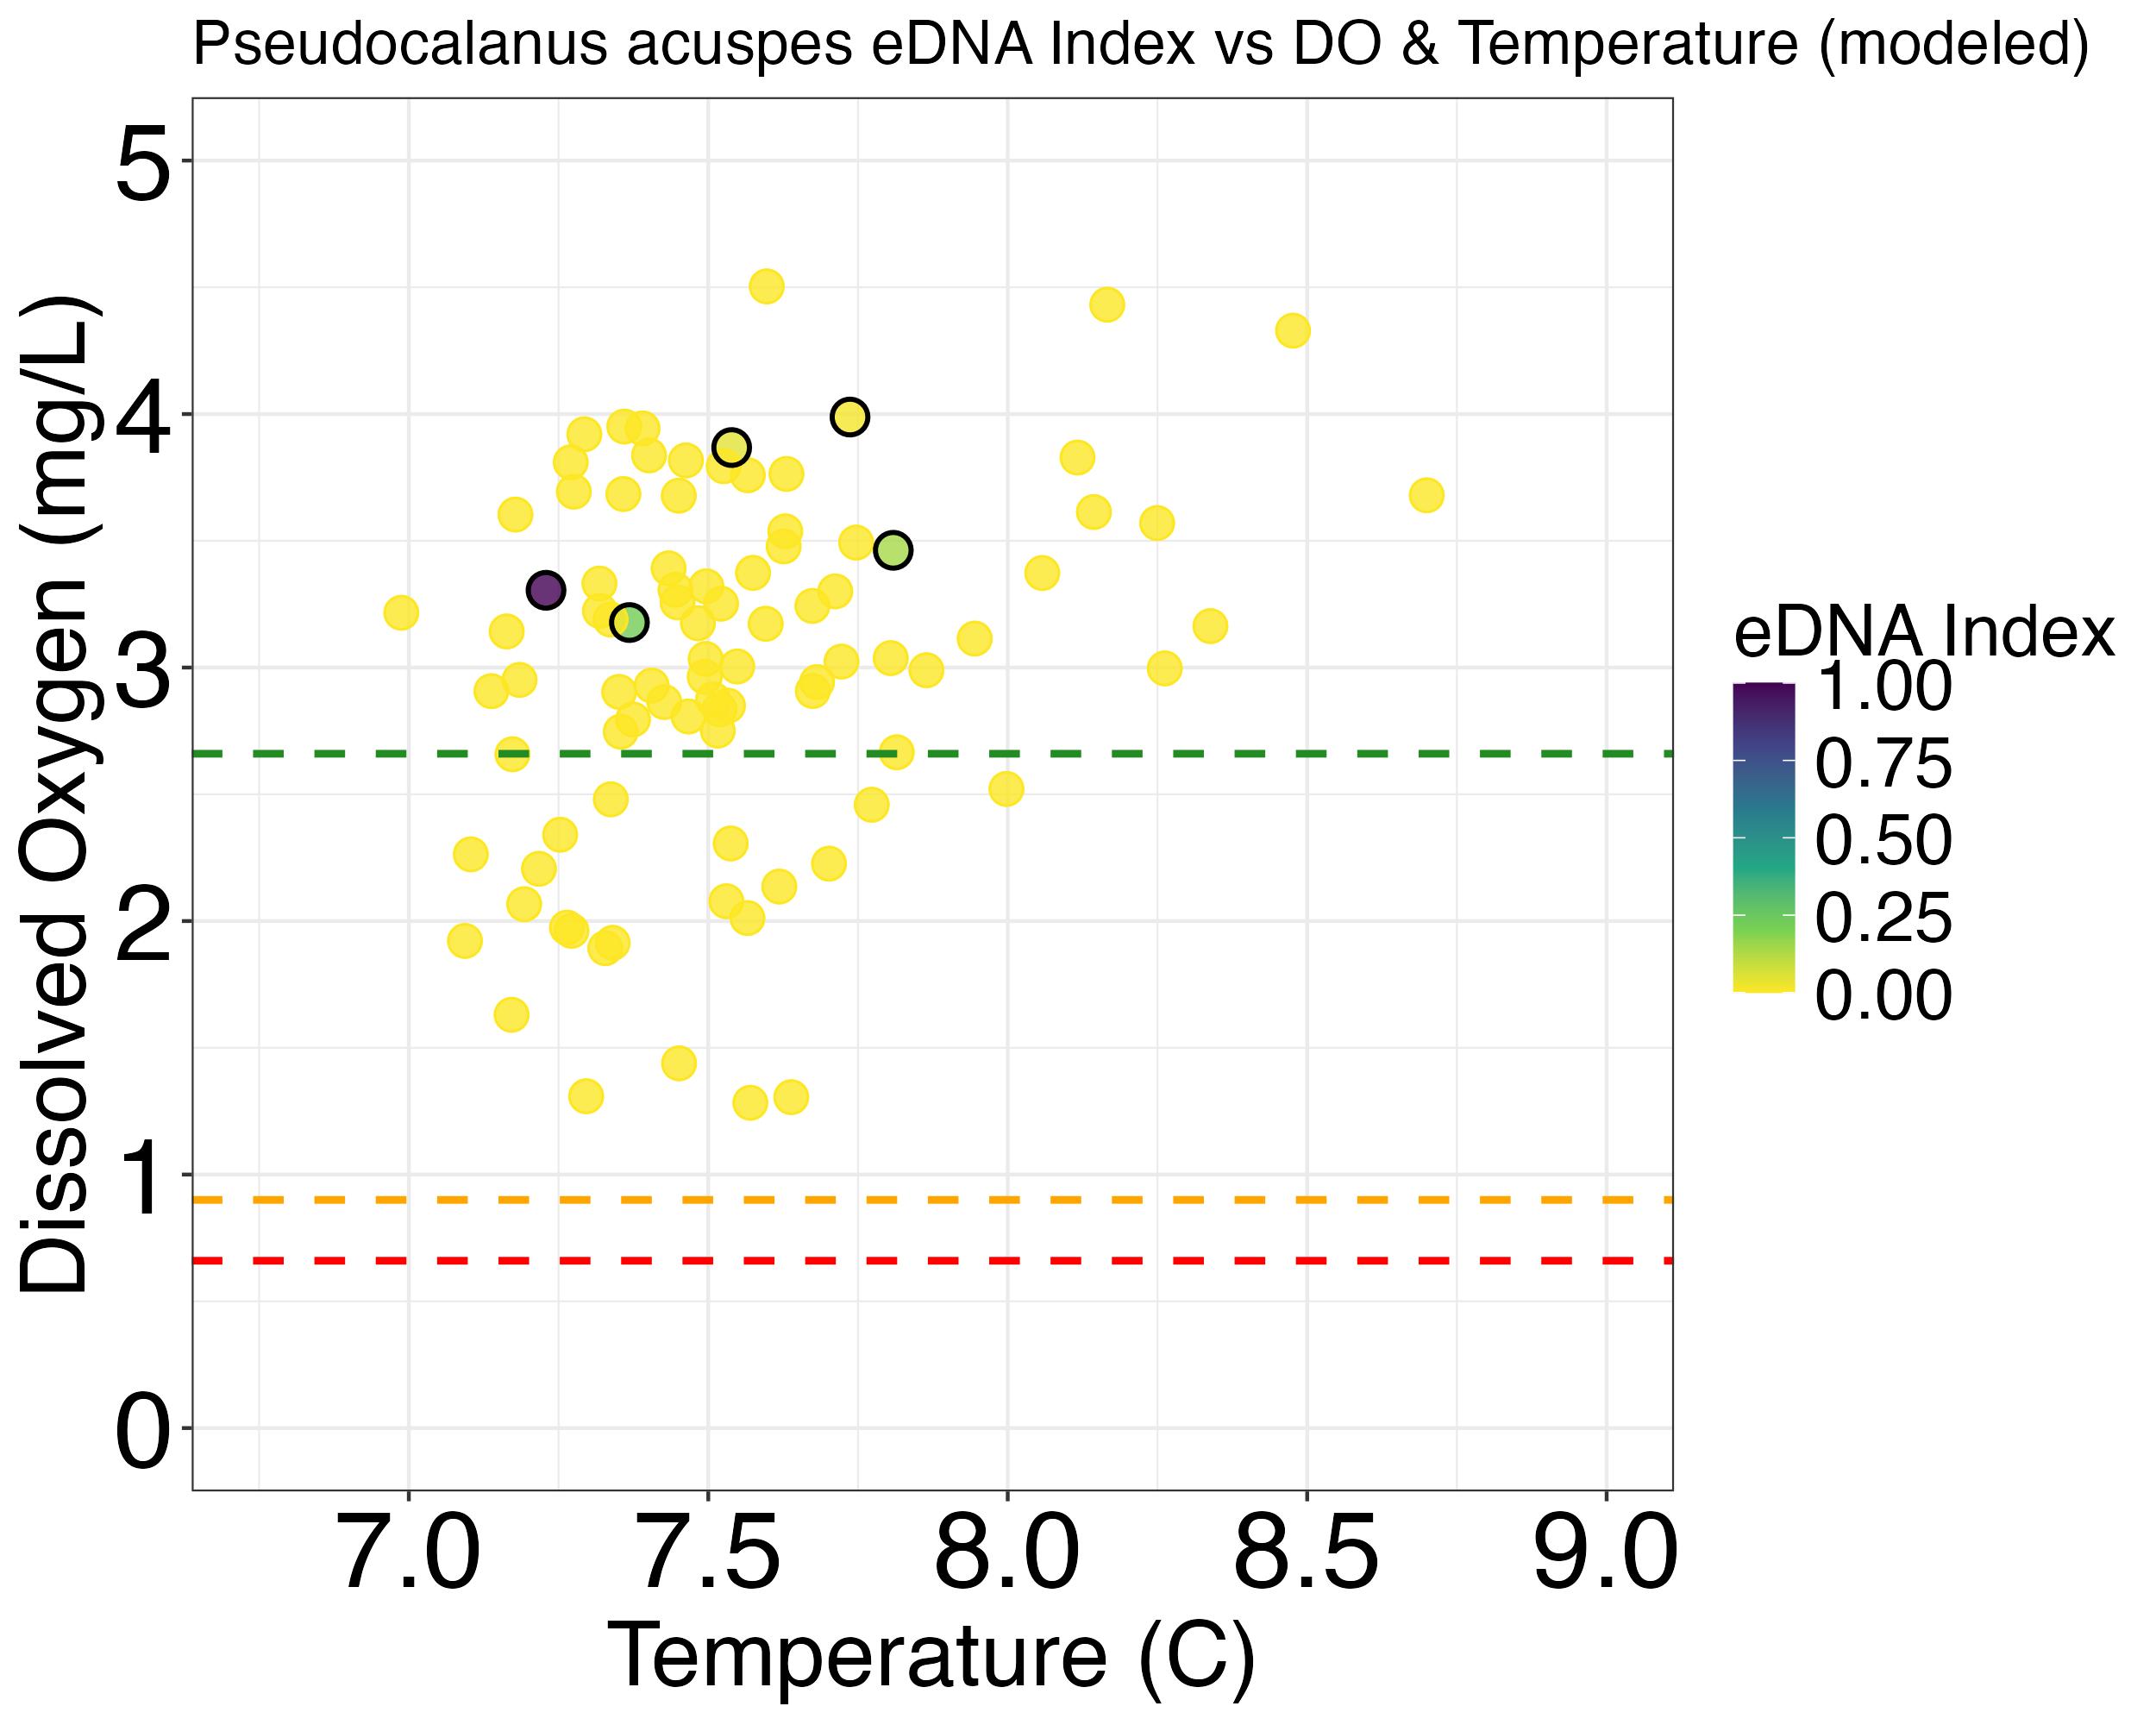
\includegraphics[scale=0.3]{Pacuspes_Scatter_AllYr_mod_noOut}
			\caption[\textit{P. acuspes} scatterplot]{\footnotesize{Scatterplot of dissolved oxygen (mg/L) and temperature (Celsius) for each environmental DNA sampling time, with \textit{P. acuspes} detections circled in black. Color of dots represents eDNA index, a normalized measure of abundance that can compare abundance within a species. Yellow, uncircled dots represent sampling dates when \textit{P. acuspes} was not detected. Plot (a) uses TH042 mooring data from 2021-22, (b) uses LiveOcean model data from 2021-23.}} %the special ToC caption is in square brackets. The \footnotesize makes the figure caption smaller
				\label{PacuspesScatter}
		\end{center}
	\end{figure} 
	
	%Southern
	
	\begin{figure}[!h]
		\begin{center}
			a. 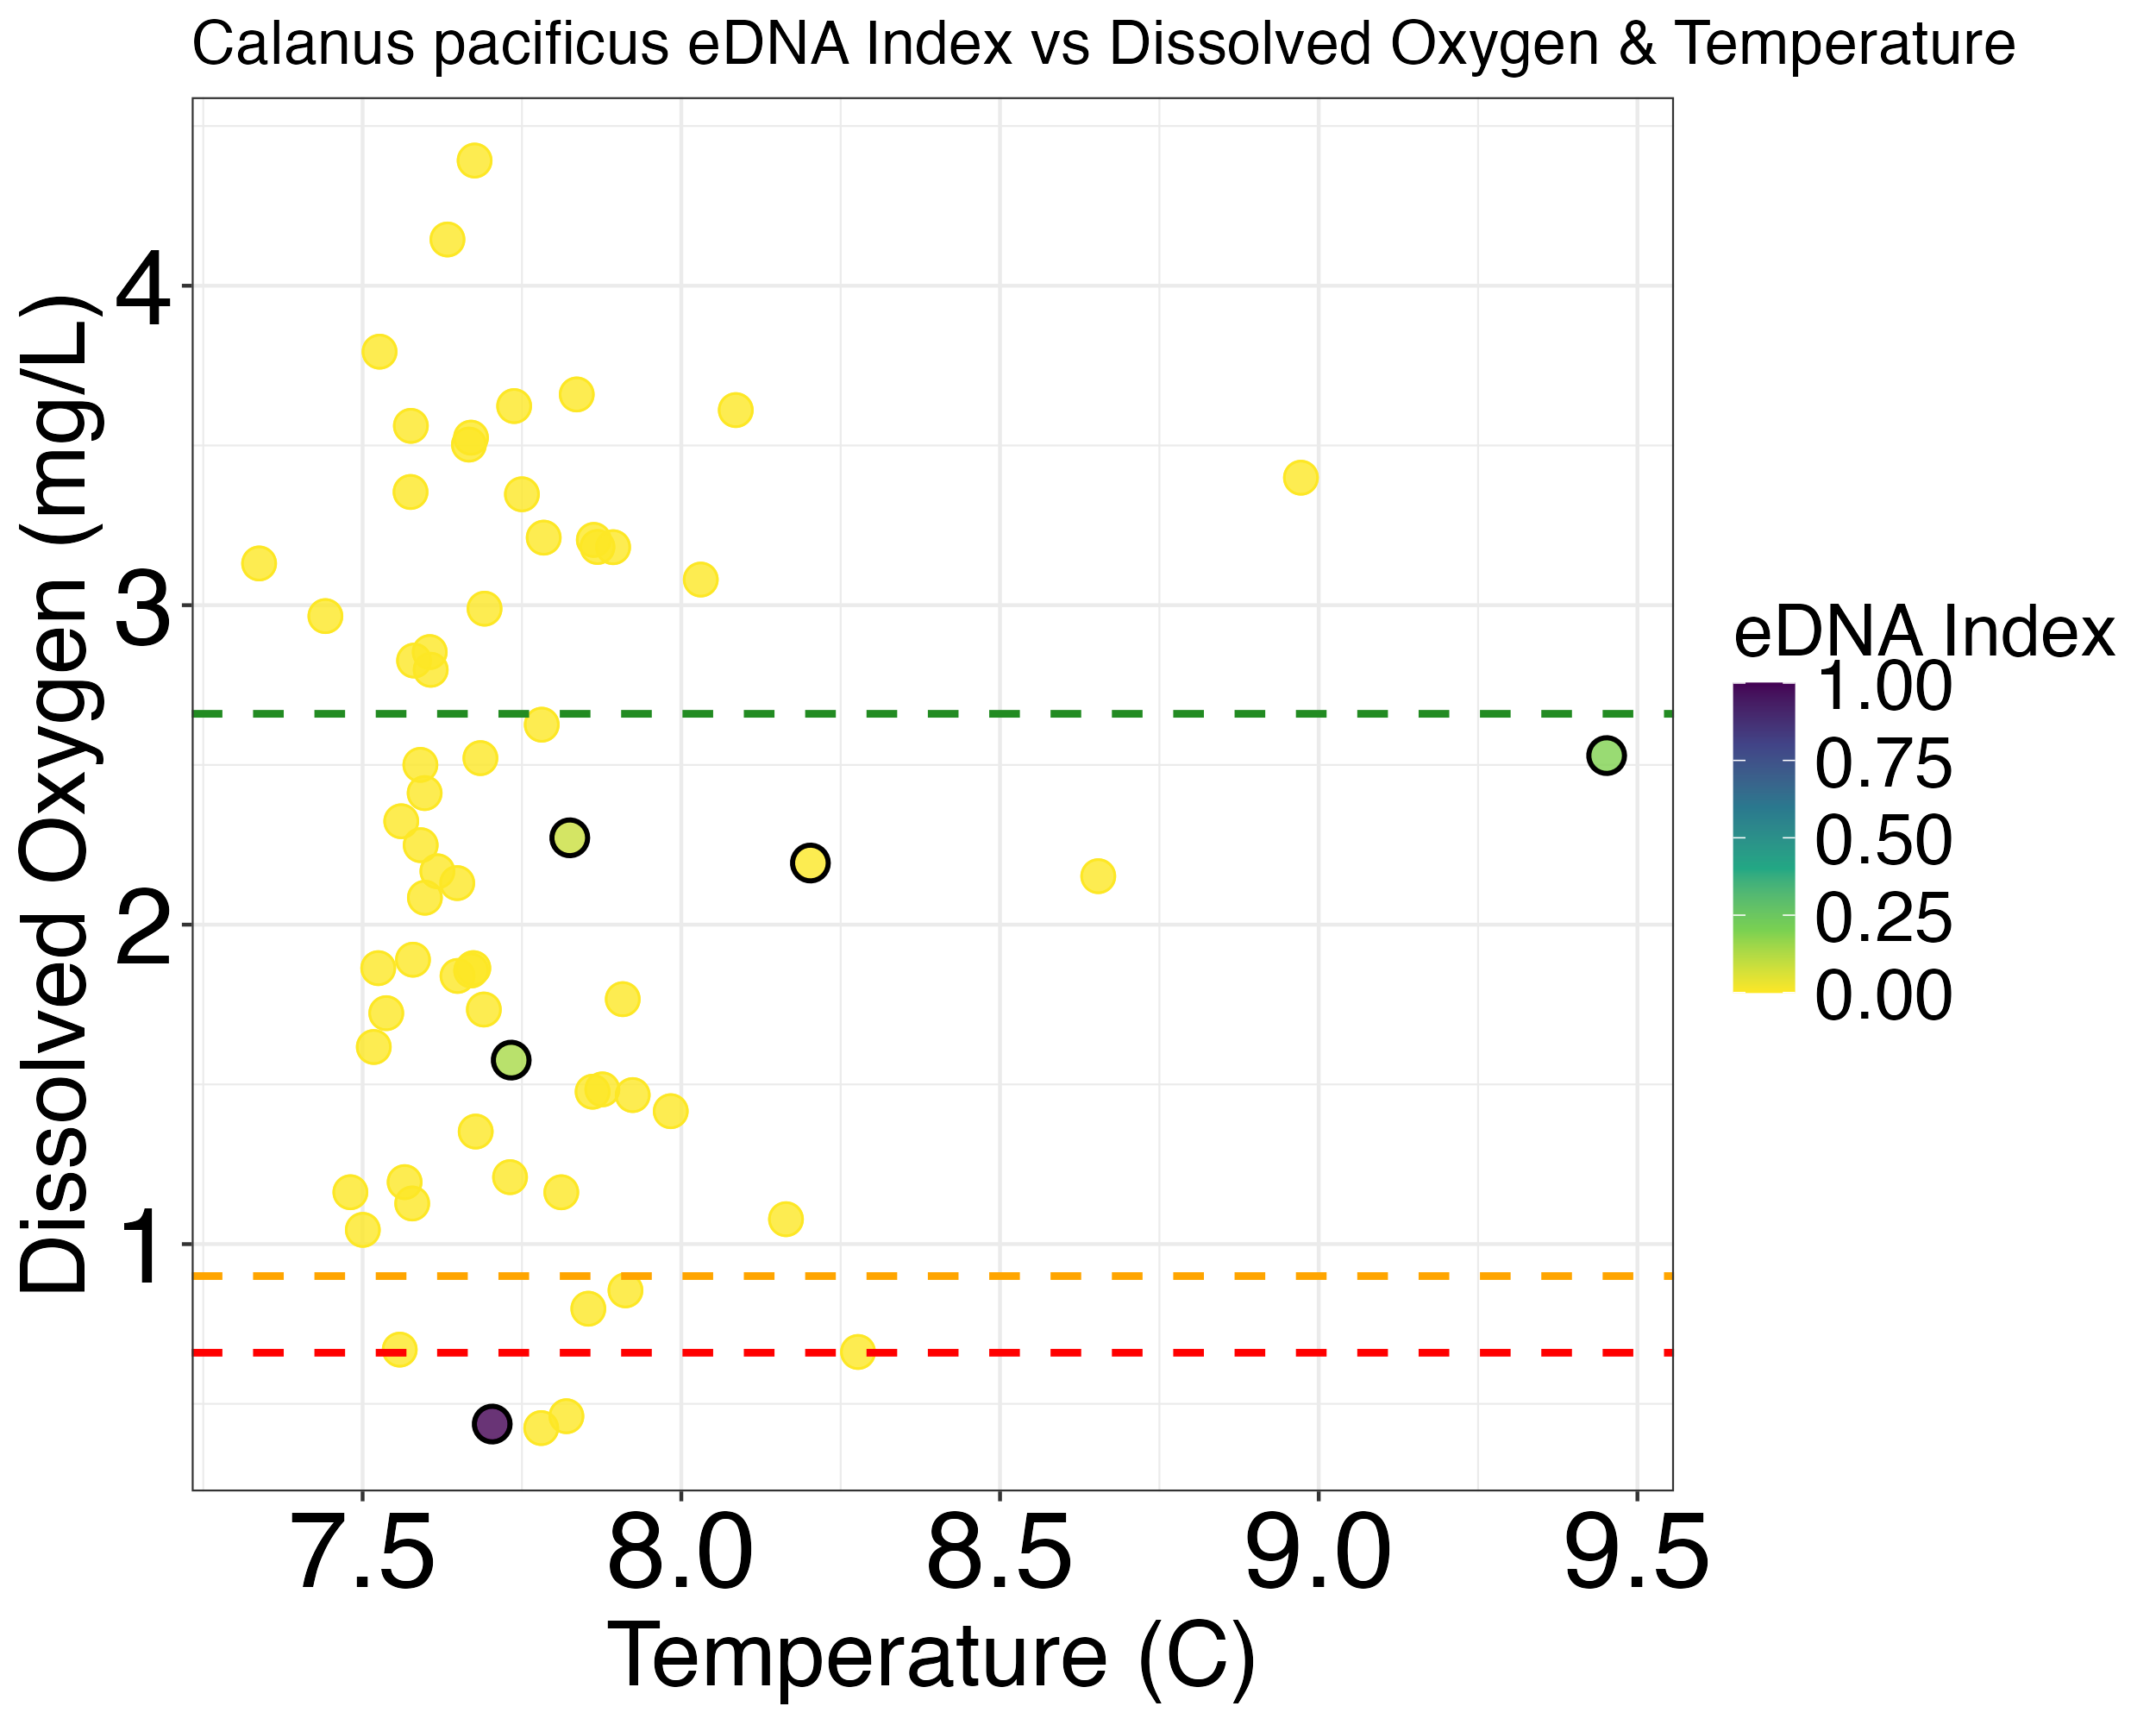
\includegraphics[scale=0.3]{Cpacificus_Scatter_noOut}
			b. 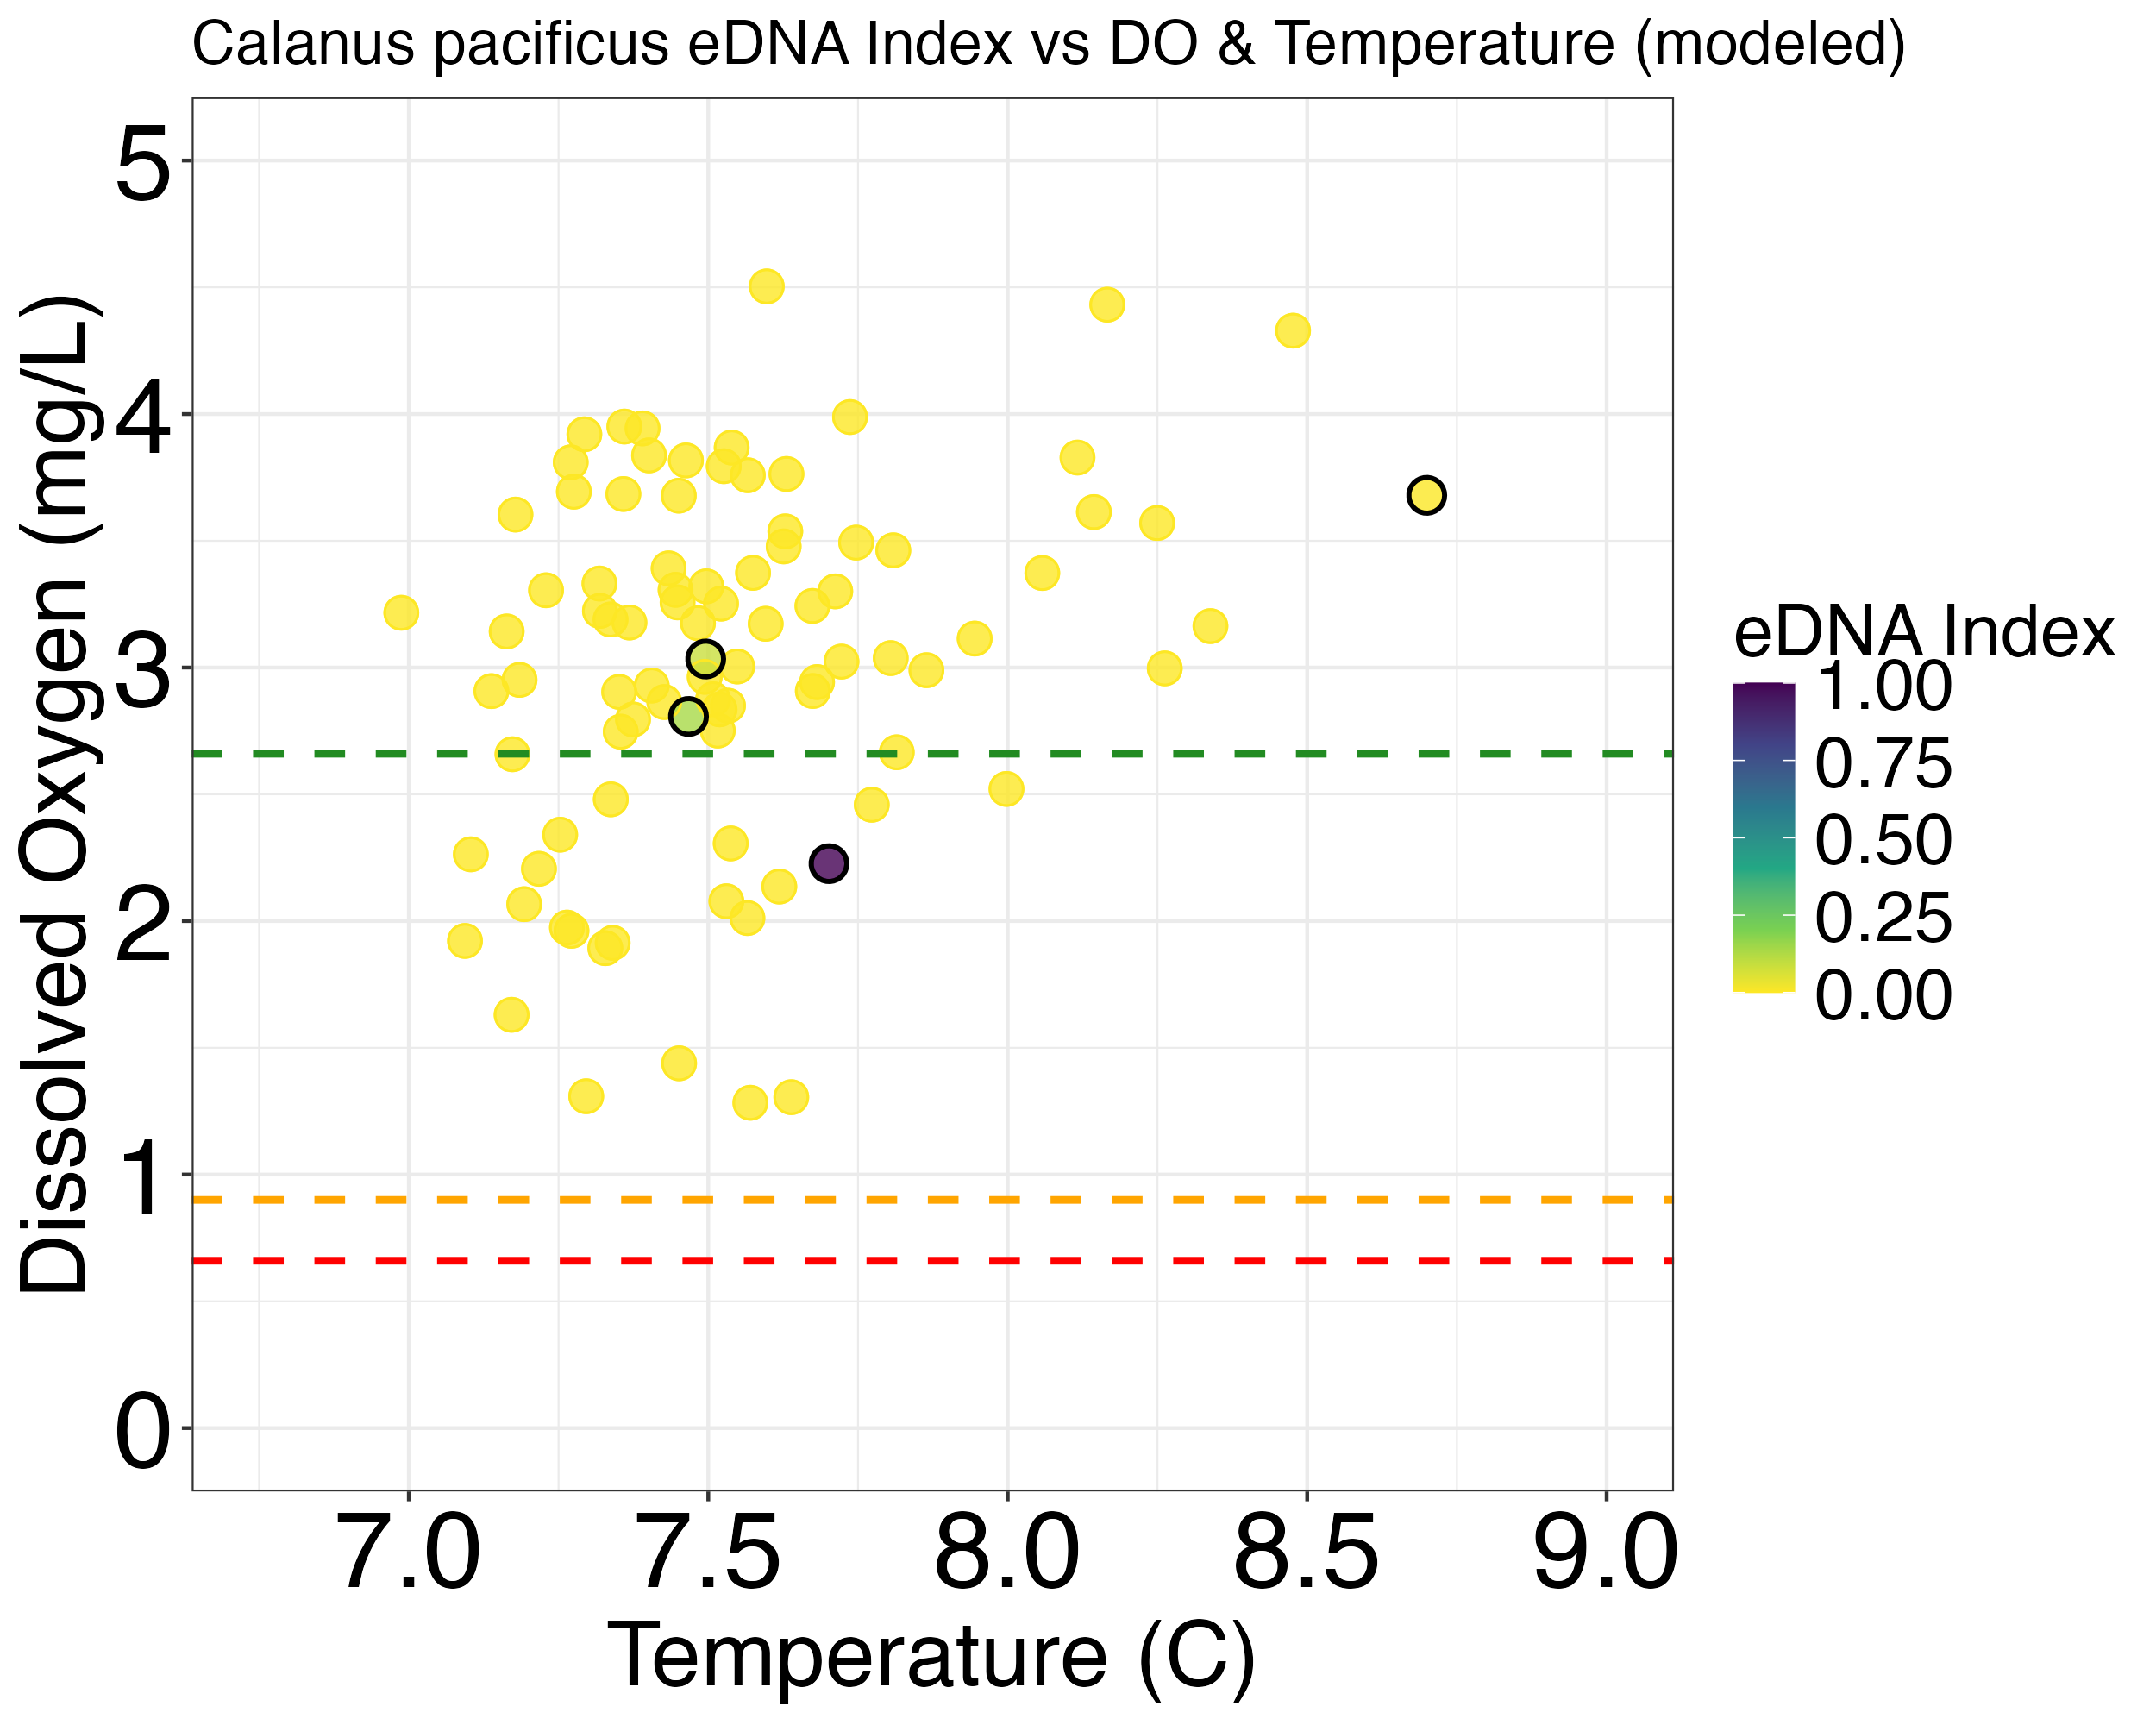
\includegraphics[scale=0.3]{Cpacificus_Scatter_AllYr_mod_noOut}
			\caption[\textit{C. pacificus} scatterplot]{\footnotesize{Scatterplot of dissolved oxygen (mg/L) and temperature (Celsius) for each environmental DNA sampling time, with \textit{C. pacificus} detections circled in black. Color of dots represents eDNA index, a normalized measure of abundance that can compare abundance within a species. Yellow, uncircled dots represent sampling dates when \textit{C. pacificus} was not detected. Plot (a) uses TH042 mooring data from 2021-22, (b) uses LiveOcean model data from 2021-23.}} %the special ToC caption is in square brackets. The \footnotesize makes the figure caption smaller
			\label{CpacificusScatter}
		\end{center}
	\end{figure} 
	
		\begin{figure}[!h]
		\begin{center}
			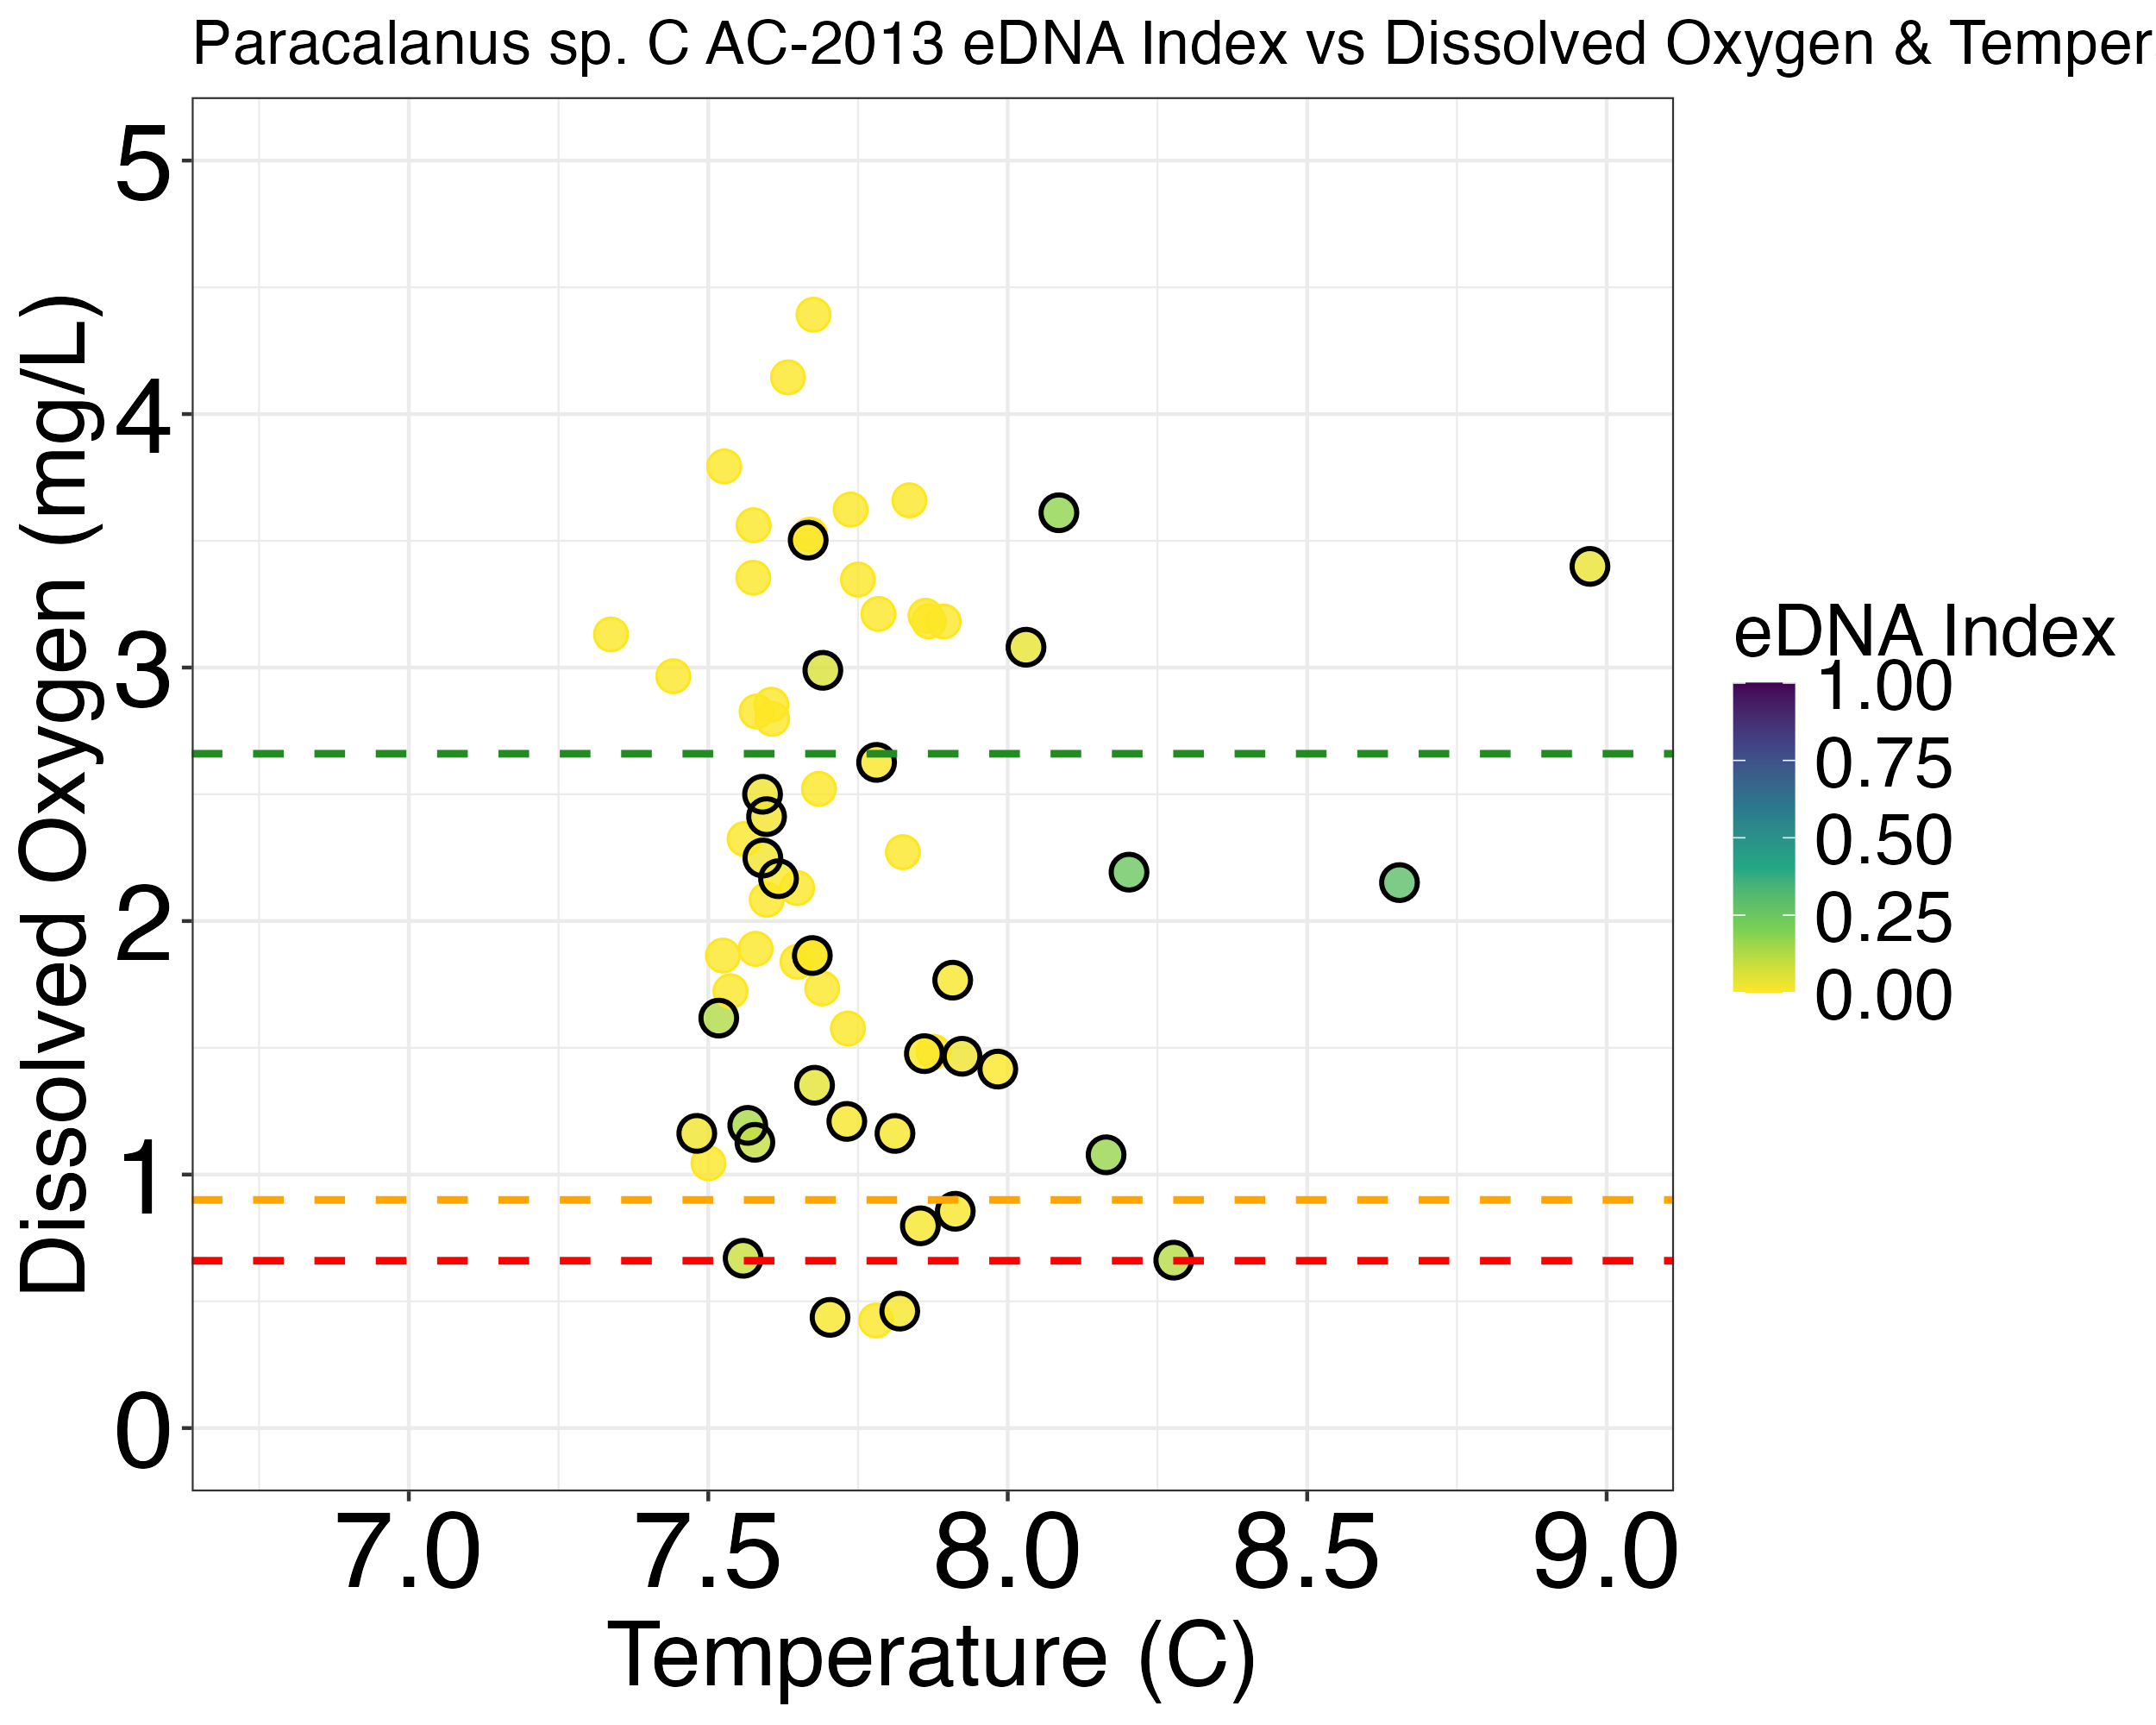
\includegraphics[scale=0.3]{Paracalanus_Scatter_noOut} \\
			\caption[\textit{Paracalanus} sp. C AC-2013 scatterplot]{\footnotesize{Scatterplot of dissolved oxygen (mg/L) and temperature (Celsius) for each environmental DNA sampling time, with \textit{Paracalanus} sp. C AC-2013 scatterplot detections circled in black. Color of dots represents eDNA index, a normalized measure of abundance that can compare abundance within a species. Yellow, uncircled dots represent sampling dates when \textit{Paracalanus} sp. C AC-2013 scatterplot was not detected. This plot uses TH042 mooring data from 2021-22.}} %the special ToC caption is in square brackets. The \footnotesize makes the figure caption smaller
			\label{ParacalanusScatterApp}
		\end{center}
	\end{figure} 
	
	\begin{figure}[!h]
		\begin{center}
			\includegraphics[scale=0.3]{Paracalanus_Density}
			\caption[\textit{Paracalanus} sp. C AC-2013 density plot (Mooring data)]{\footnotesize{Density plot of \textit{Paracalanus} sp. C AC-2013 detections. Each pixel represents a range of dissolved oxygen and temperature values, and the shade of each pixel represents the proportion of eDNA samples in that environmental range in which \textit{Paracalanus} sp. C AC-2013 was detected. This plot uses TH042 mooring data from 2021-22.}} %the special ToC caption is in square brackets. The \footnotesize makes the figure caption smaller
			\label{ParacalanusDensityMod}
		\end{center}
	\end{figure}

  \backmatter % backmatter makes the index and bibliography appear properly in the t.o.c...

% if you're using bibtex, the next line forces every entry in the bibtex file to be included
% in your bibliography, regardless of whether or not you've cited it in the thesis.
%    \nocite{*}

% Rename my bibliography to be called "Works Cited" and not "References" or ``Bibliography''
 \renewcommand{\bibname}{Works Cited}

%\bibliographystyle{APA/apa-good}  % or
% \bibliography{thesis}
 % Comment the above two lines and uncomment the next line to use biblatex-chicago.
\printbibliography[heading=bibintoc, notcategory=nobibliography]

% Finally, an index would go here... but it is also optional.
\end{document}
